\label{sec:rawDataMCComparisons}
\label{sec:dijetresults}

\ifnpas
In this Section, the detector-level distributions of the jet mass
are investigated. Each of the distributions are made for 
the $\pt^{AVG}$ bins described in Section~\ref{sec:ptBinAssignment}. 
Each of the figures shows the raw event counts per $\pt^{AVG}$ bin,
as a function of the average jet mass $m_J^{AVG}$. 


Figure~\ref{figs:histAK7PtAvgVsMjetGroomOverReco_ratioPlots}
shows a comparison of the jet mass from the groomed jets
divided by the jet mass of matched ungroomed jets, for the
three grooming techniques, for both data and the \PYTHIA Monte Carlo. 
The data and the MC both exhibit similar behavior. In general,
the filtering algorithm (black) is the least aggressive grooming technique,
with groomed jet masses close to the ungroomed case.
The trimming algorithm (red) is moderately aggressive, and the
pruning algorithm (blue) is the most aggressive. In the case of
the pruning algorithm, a bimodal distribution begins to manifest,
which is typical of this algorithm since the parameters we have
chosen require two subjets to be created. In the cases where
the pruned jet mass is close to the ungroomed jet mass, 
jets usually have large ``core'' components
and small amounts of radiation, whereas when the pruned jet
mass is closer to 0, the jets are more symmetrically split
due to gluons splitting into two jets that fall within
our $D=0.7$ parameter. 
\fi

\ifnpas
Figures~\ref{figs:histAK7MjetVsPtAvg_rawDataMCComparisons_stacktrigs_pt_2}-
\ref{figs:histAK7MjetVsPtAvg_rawDataMCComparisons_stacktrigs_pt_5}
show the jet mass distribution for AK7 jets, along with
the trigger breakdown for all of the $\pt^{AVG}$ bins. In each case,
only one trigger contributes to any given $\pt^{AVG}$ bin. 


Figures~\ref{figs:histAK7MjetVsPtAvg_rawDataMCComparisons_pt_2}-
\ref{figs:histAK7MjetVsPtAvg_rawDataMCComparisons_pt_2_Pruned}
%\ref{figs:histAK7MjetVsPtAvg_rawDataMCComparisons_pt_5_Pruned}
show the detector-level distributions for the various jet grooming
algorithms, compared to predictions from \PYTHIA, \PYTHIA8, and
\HERWIG Monte Carlo samples. Each MC sample is normalized
according to the expected luminosity and computed cross sections. 
\fi

\ifnpas

\begin{figure}[htbp]
\centering
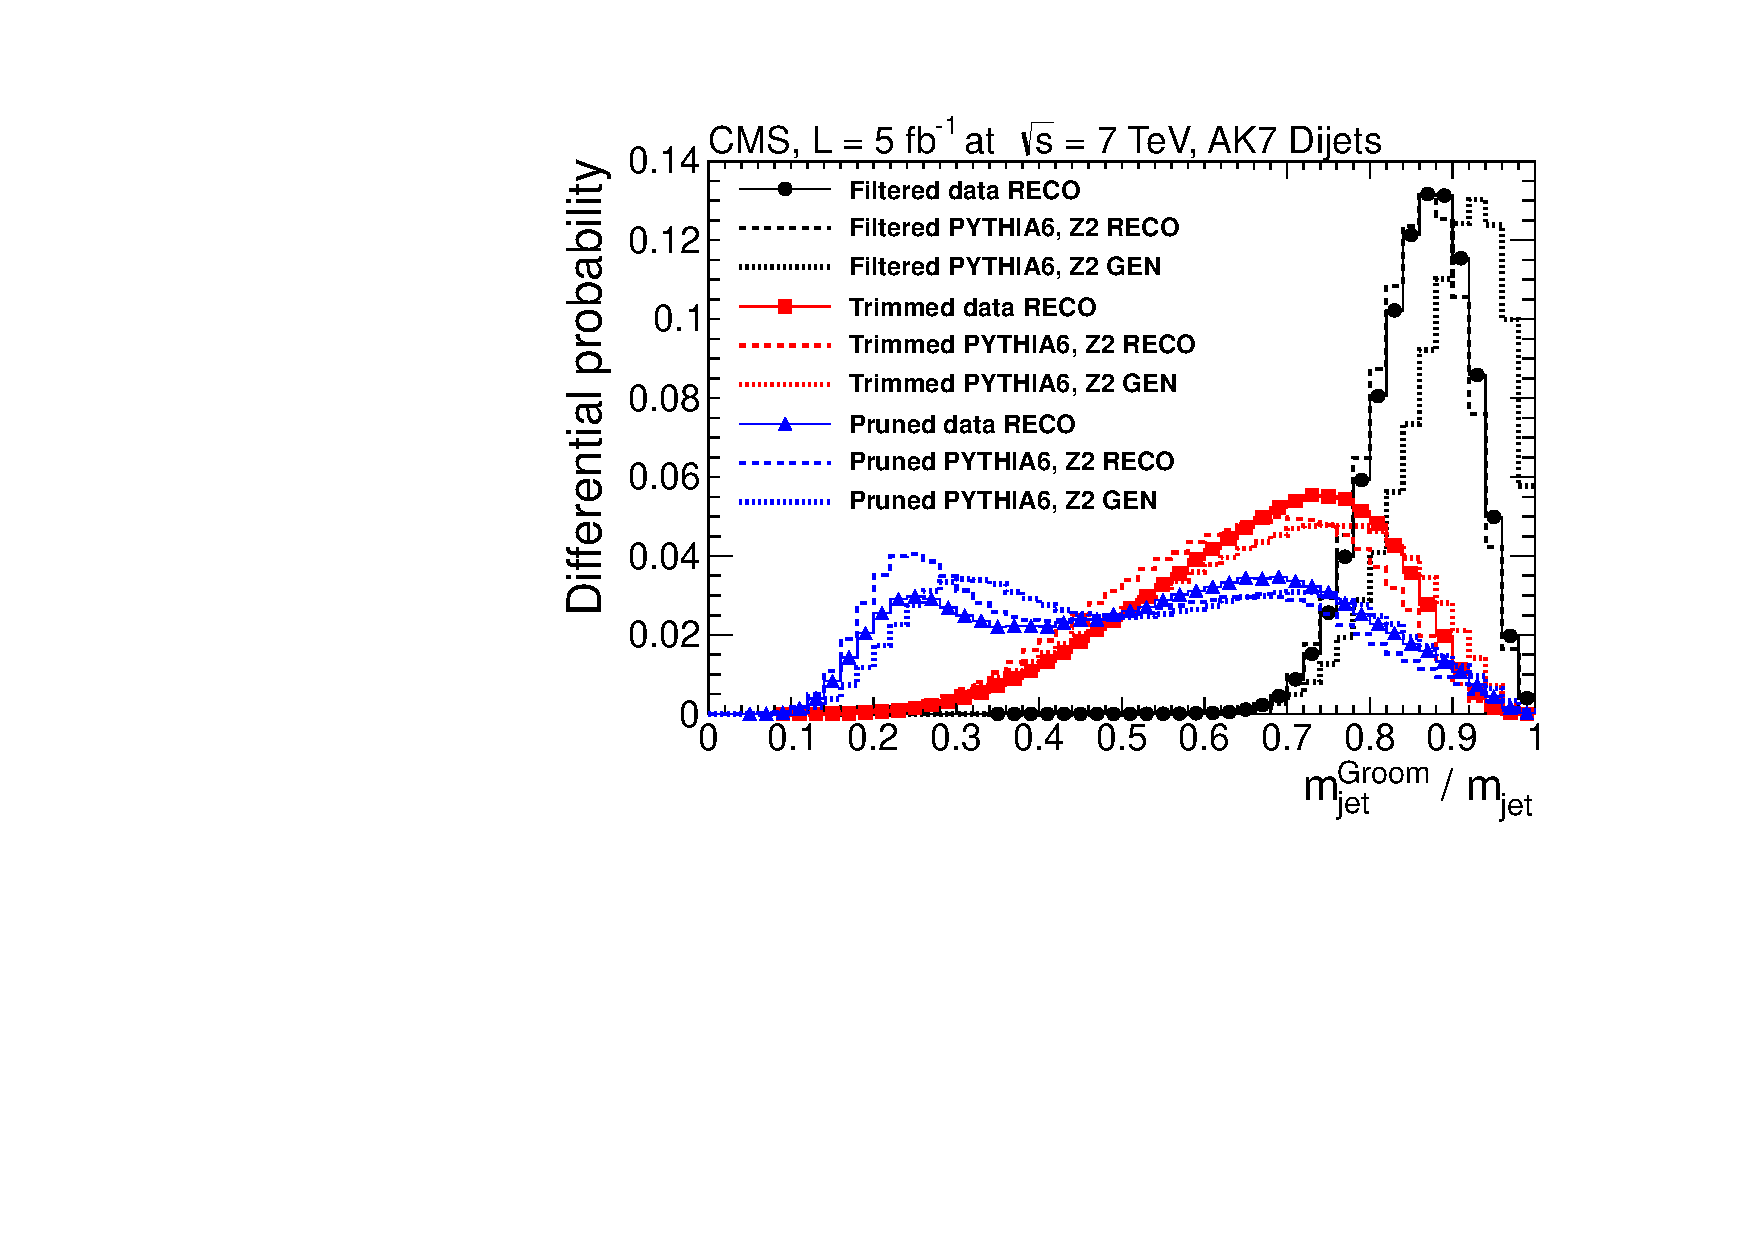
\includegraphics[width=0.95\textwidth]{figs/histAK7PtAvgVsMjetGroomOverReco_ratioPlots}
\caption{Comparison of the jet mass from the groomed jets
divided by the jet mass of matched ungroomed jets for the
three grooming techniques, for both data and the \PYTHIA Monte Carlo. 
\label{figs:histAK7PtAvgVsMjetGroomOverReco_ratioPlots}}
\end{figure}

\fi


\label{sec:results}

\ifnpas
The unfolded distributions of the 
averge jet mass are also investigated.
In Figures~\ref{figs:unfoldedMeasurementDijets_1_allsys}-
\ref{figs:unfoldedMeasurementDijets_9_Pruned_allsys}, 
the differential cross
section from Eq.(\ref{eq:pdf_mjet_simple}) is shown for
various $\pt^{AVG}$ bins, as a function of
$m_{J}^{AVG}$, as described in
Section~\ref{sec:dataSampleAndEventSelection}, 
for ungroomed jets and for different grooming algorithms. 
As described in Eq.(\ref{eq:pdf_mjet_simple}),
each distribution in each $\pt^{AVG}$ is separately normalized to
unity, and each bin content is divided by the bin width of the
$m_J^{AVG}$ bin,
so these plots show the probability distribution function of $m_J^{AVG}$,
with units of 1/GeV (see Eq.(~\ref{eq:pdf_mjet_simple})). 
The shapes for $m_J^{AVG}$ in the MC samples are
taken directly from the MC.


The statistical uncertainty is shown in light shading, the uncertainties due to the jet-energy resolution, jet-energy scale, and jet-angular resolution are shown in shades of brown, the uncertainty due to pileup is shown in green, and the uncertainty due to the parton shower differences are shown in dark shading.
The simulated distribution from \PYTHIA is shown in solid lines, 
from \PYTHIAEIGHT in dashed lines, and from \HERWIG in dotted lines. 
The bottom frame shows the ratio of the true distribution from
the simulation divided by the unfolded distribution, along with
the uncertainties in the unfolded distribution. 


Figures~\ref{figs:unfoldedMeasurementDijets_1}-
\ref{figs:unfoldedMeasurementDijets_9_Pruned}, 
show the same plots, however in a simplified format with only the
total and statistical uncertainties shown in dark shading and 
light shading, respectively. 
\fi

\ifpas

%The unfolded distributions of the 
%average jet mass are also investigated.
The differential probability distributions of Eq.~(\ref{eq:pdf_mjet_simple}) 
for $m_J^{AVG}$ of the two leading jets in dijet events,
corrected for detector effects in the jet mass, are displayed in
Figs.~\ref{figs:unfoldedMeasurementDijets_all}--\ref{figs:unfoldedMeasurementDijets_all_Pruned}
%\ref{figs:unfoldedMeasurementDijets_5_Pruned}, 
for seven bins in $\pt^{AVG}$ along with the \HERWIG predictions..
The $\pt^{AVG}$ is 
not corrected to the particle level, because the correction is
expected to be negligible for the momenta considered.
Results are shown
for ungroomed jets and for the three categories of grooming. 
%As described in Sec.~\ref{sec:intro},
Each distribution is normalized to unity.
%, and each bin content is divided by the bin width of the
%$m_J^{AVG}$ bin,
%so these plots show the probability distribution function of $m_J^{AVG}$,
%with units of 1/GeV. % (see Eq.~\ref{eq:pdf_mjet_simple}). 
%The shapes for $m_J^{AVG}$ in the MC samples are
%taken directly from the MC. 
%%The unfolded data are given by the indicated symbols, and the 
%%total and statistical uncertainties on each point are shown,
%%respectively, as dark shading and 
%%light shadings, respectively. The \HERWIG  prediction is shown
%%as a dotted line. 
%Figures~\ref{figs:unfoldedMeasurementDijets_allfrac}-
%\ref{figs:unfoldedMeasurementDijets_allfrac_Pruned},
The ratios of the MC simulations used in
Figs.~\ref{figs:unfoldedMeasurementDijets_all}--\ref{figs:unfoldedMeasurementDijets_all_Pruned}
to the results for data, for \PYTHIA, \PYTHIAEIGHT, and for \HERWIG are given in Figs.~\ref{figs:unfoldedMeasurementDijets_allfrac}--\ref{figs:unfoldedMeasurementDijets_allfrac_Pruned}, respectively. 

\fi 

The largest systematic uncertainty is from the choice of parton-shower modeling used to calculate detector corrections, with
small, but still significant uncertainties arising from jet energy scale and resolution, and
small contributions from jet angular resolution and pileup. 
In the 220--300\GeV and 300--450\GeV jet-$\pt$ bins, the $m_J < 50\GeV$ region 
is dominated by uncertainties from unfolding (50--100\%), which are
negligible for $\pt^{AVG}>450\GeV$. 
For $m_J > 50\GeV$, the JES, JER, JAR, and pileup uncertainties each
contribute ${\approx} 10\%$. For the 
450--1000\GeV $\pt$ bins, parton
showering dominates the uncertainties, which is around 50--100\% below
the peak of the $m_J$
distribution and 5--10\% for the rest of the distribution. For 
$\pt > 1000 \GeV$, statistical uncertanty dominates the entire mass range.

For clarity, the distributions in 
Figs.~\ref{figs:unfoldedMeasurementDijets_allfrac}--\ref{figs:unfoldedMeasurementDijets_allfrac_Pruned} 
are truncated where few events are recorded.
Bins in $m_J^{AVG}$ with uncertainties of $>$ 100\% are
ignored to avoid overlap with more precise measurements in other
$\pt^{AVG}$ bins. 
The agreement with \HERWIG modeling of parton showers appears to be 
best for $\pt^{AVG}>300\GeV$ and $m_{J}^{AVG}>20\GeV$.
% Above $\pt^{AVG} > 300$ \GeV, the 
%\HERWIG model seems to describe the jet mass very well above
%$m_{J}^{AVG} > 50$ \GeV. 
%After applying the various grooming techniques,
%the agreement is even improved, and the agreement begins
%at around $m_{J}^{AVG} > 20$ \GeV. 
However, the ungroomed and filtered jets show worse agreement 
for $20<m_{J}^{AVG}<50\GeV$ when $\pt^{AVG}>450\GeV$.
For all generators and all $\pt^{AVG}$ bins, the agreement is better
at larger jet masses. The disagreement is largest at the very lowest
mass values, which correspond to the region most sensitive to 
the underlying event description and pileup, 
and where the amount of showering is apparently underestimated in the
simulation. 

%


\begin{figure}[htbp]
\centering
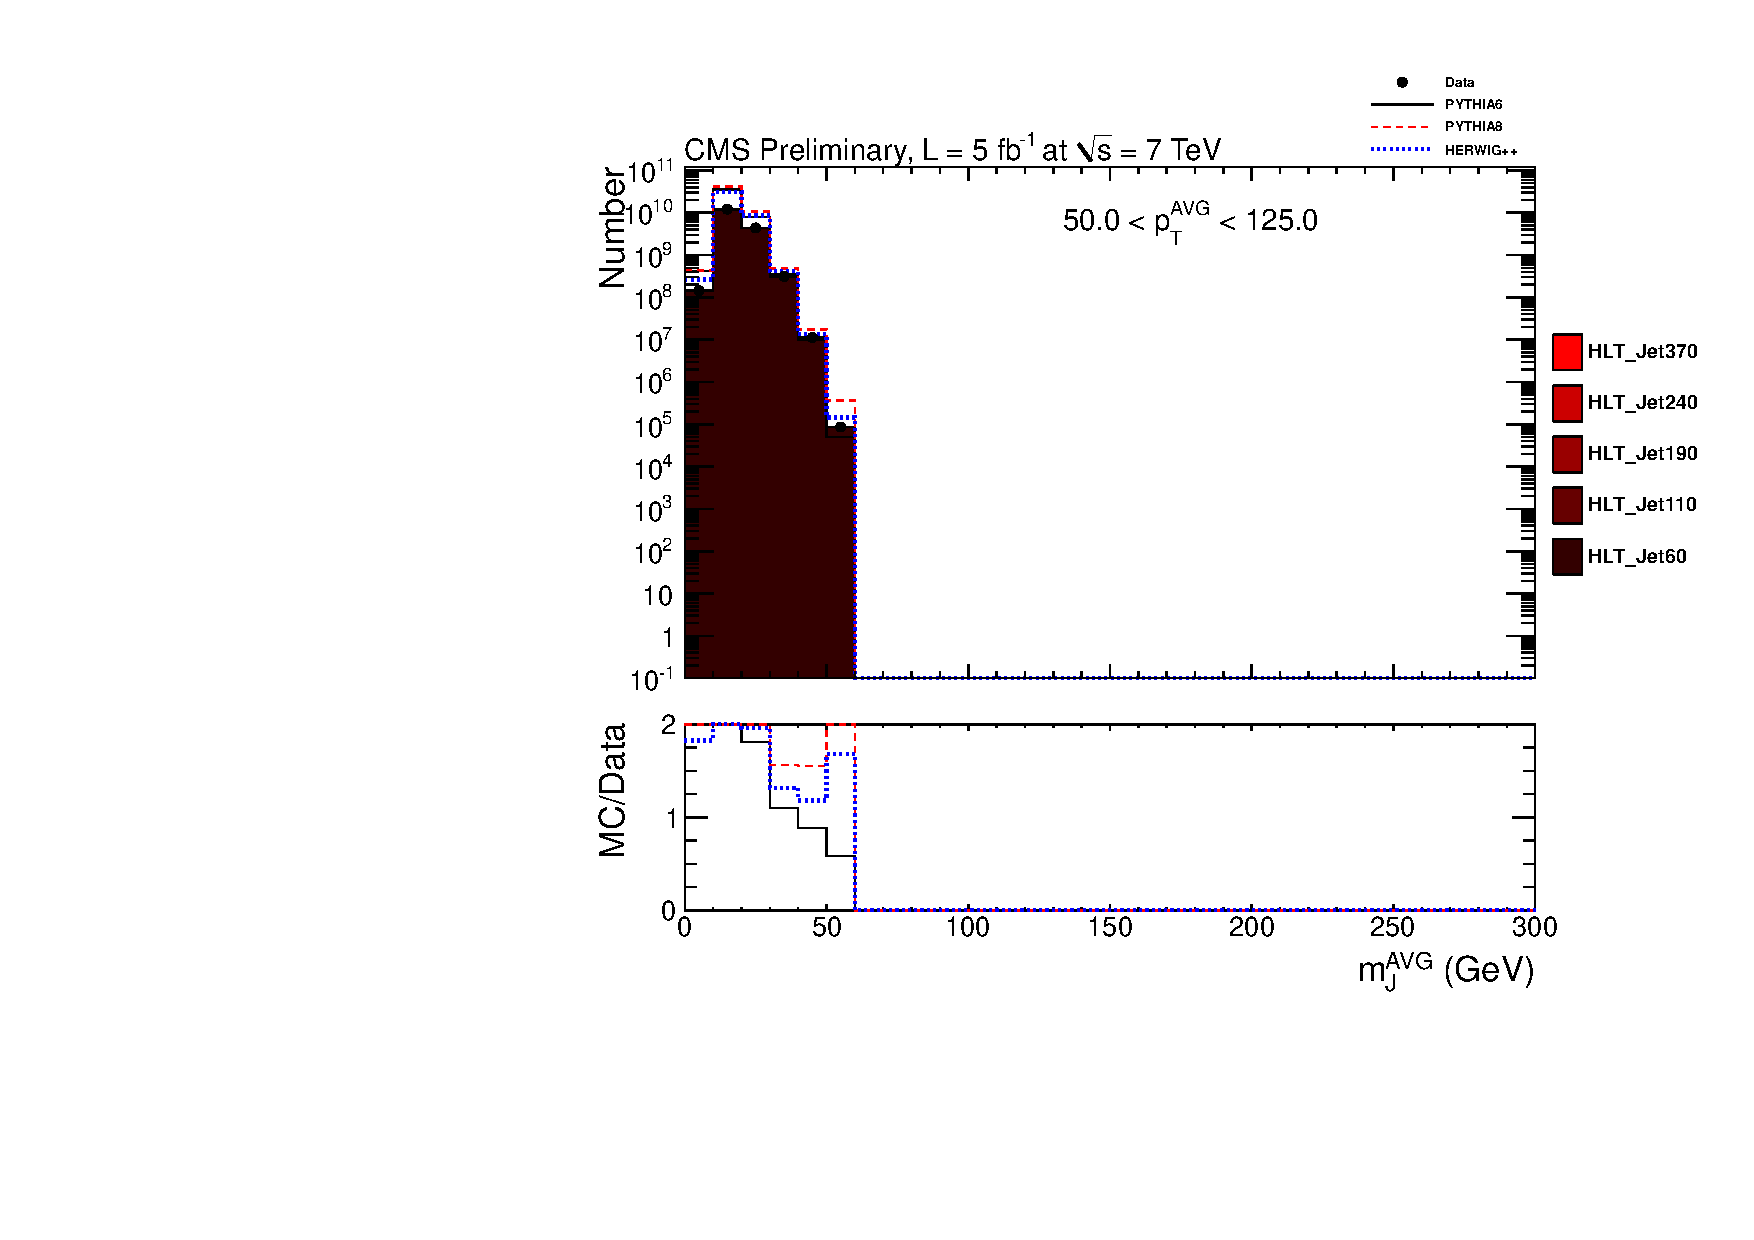
\includegraphics[width=0.95\textwidth]{figs/histAK7MjetVsPtAvg_rawDataMCComparisons_stacktrigs_pt_1}
\caption{Detector-level distributions of the jet mass for AK7 jets,
for $50.0 < \pt^{AVG} < 125.0$ \GeVc. The data are shown in black points.
The simulated distribution from \PYTHIA is shown in solid black, 
the from \PYTHIAEIGHT in dashed red, and from \HERWIG in dotted blue. 
The bottom frame shows the ratio of the simulated distribution
to the distribution from data. The various trigger contributions are shown in shades of red.
\label{figs:histAK7MjetVsPtAvg_rawDataMCComparisons_stacktrigs_pt_1}}
\end{figure}



\begin{figure}[htbp]
\centering
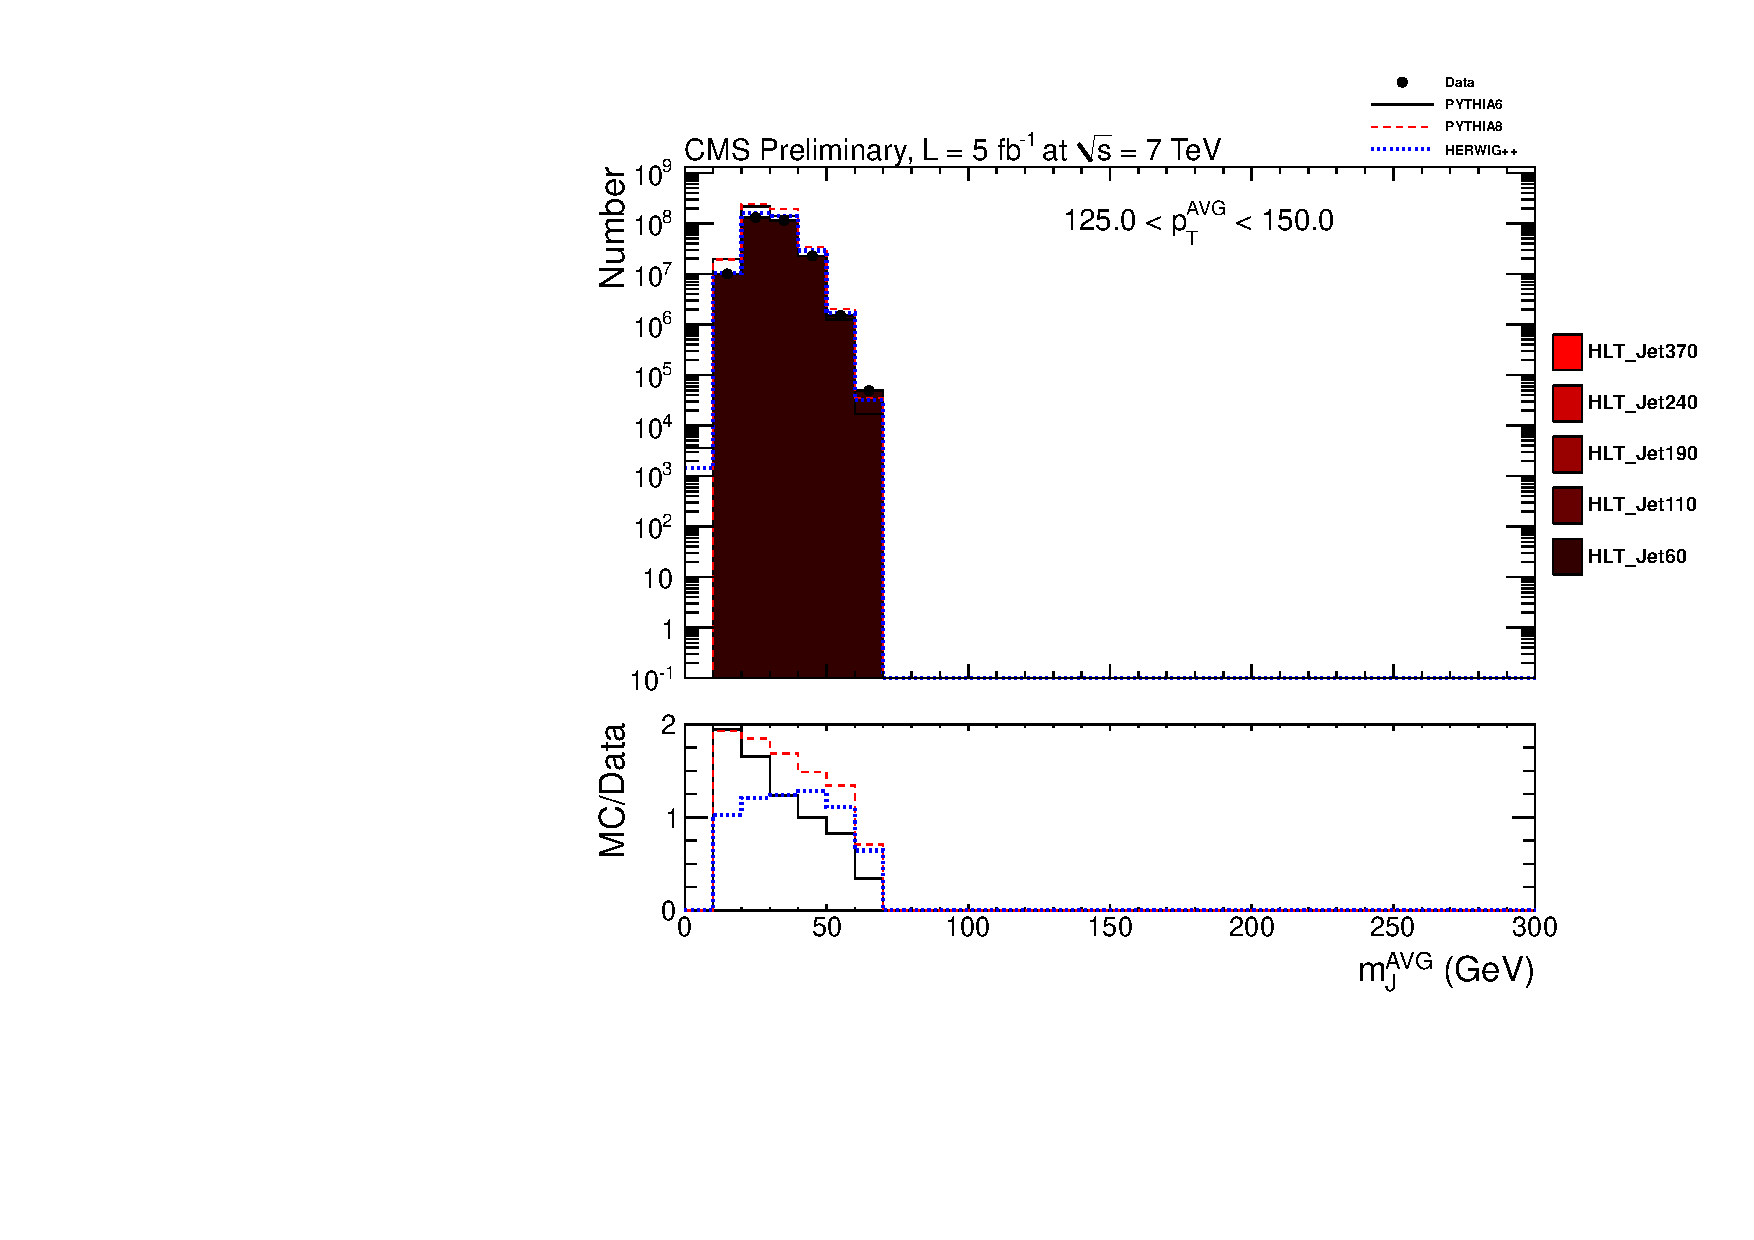
\includegraphics[width=0.95\textwidth]{figs/histAK7MjetVsPtAvg_rawDataMCComparisons_stacktrigs_pt_2}
\caption{Detector-level distributions of the jet mass for AK7 jets,
for $125.0 < \pt^{AVG} < 150.0$ \GeVc. The data are shown in black points.
The simulated distribution from \PYTHIA is shown in solid black, 
the from \PYTHIAEIGHT in dashed red, and from \HERWIG in dotted blue. 
The bottom frame shows the ratio of the simulated distribution
to the distribution from data. The various trigger contributions are shown in shades of red.
\label{figs:histAK7MjetVsPtAvg_rawDataMCComparisons_stacktrigs_pt_2}}
\end{figure}



\begin{figure}[htbp]
\centering
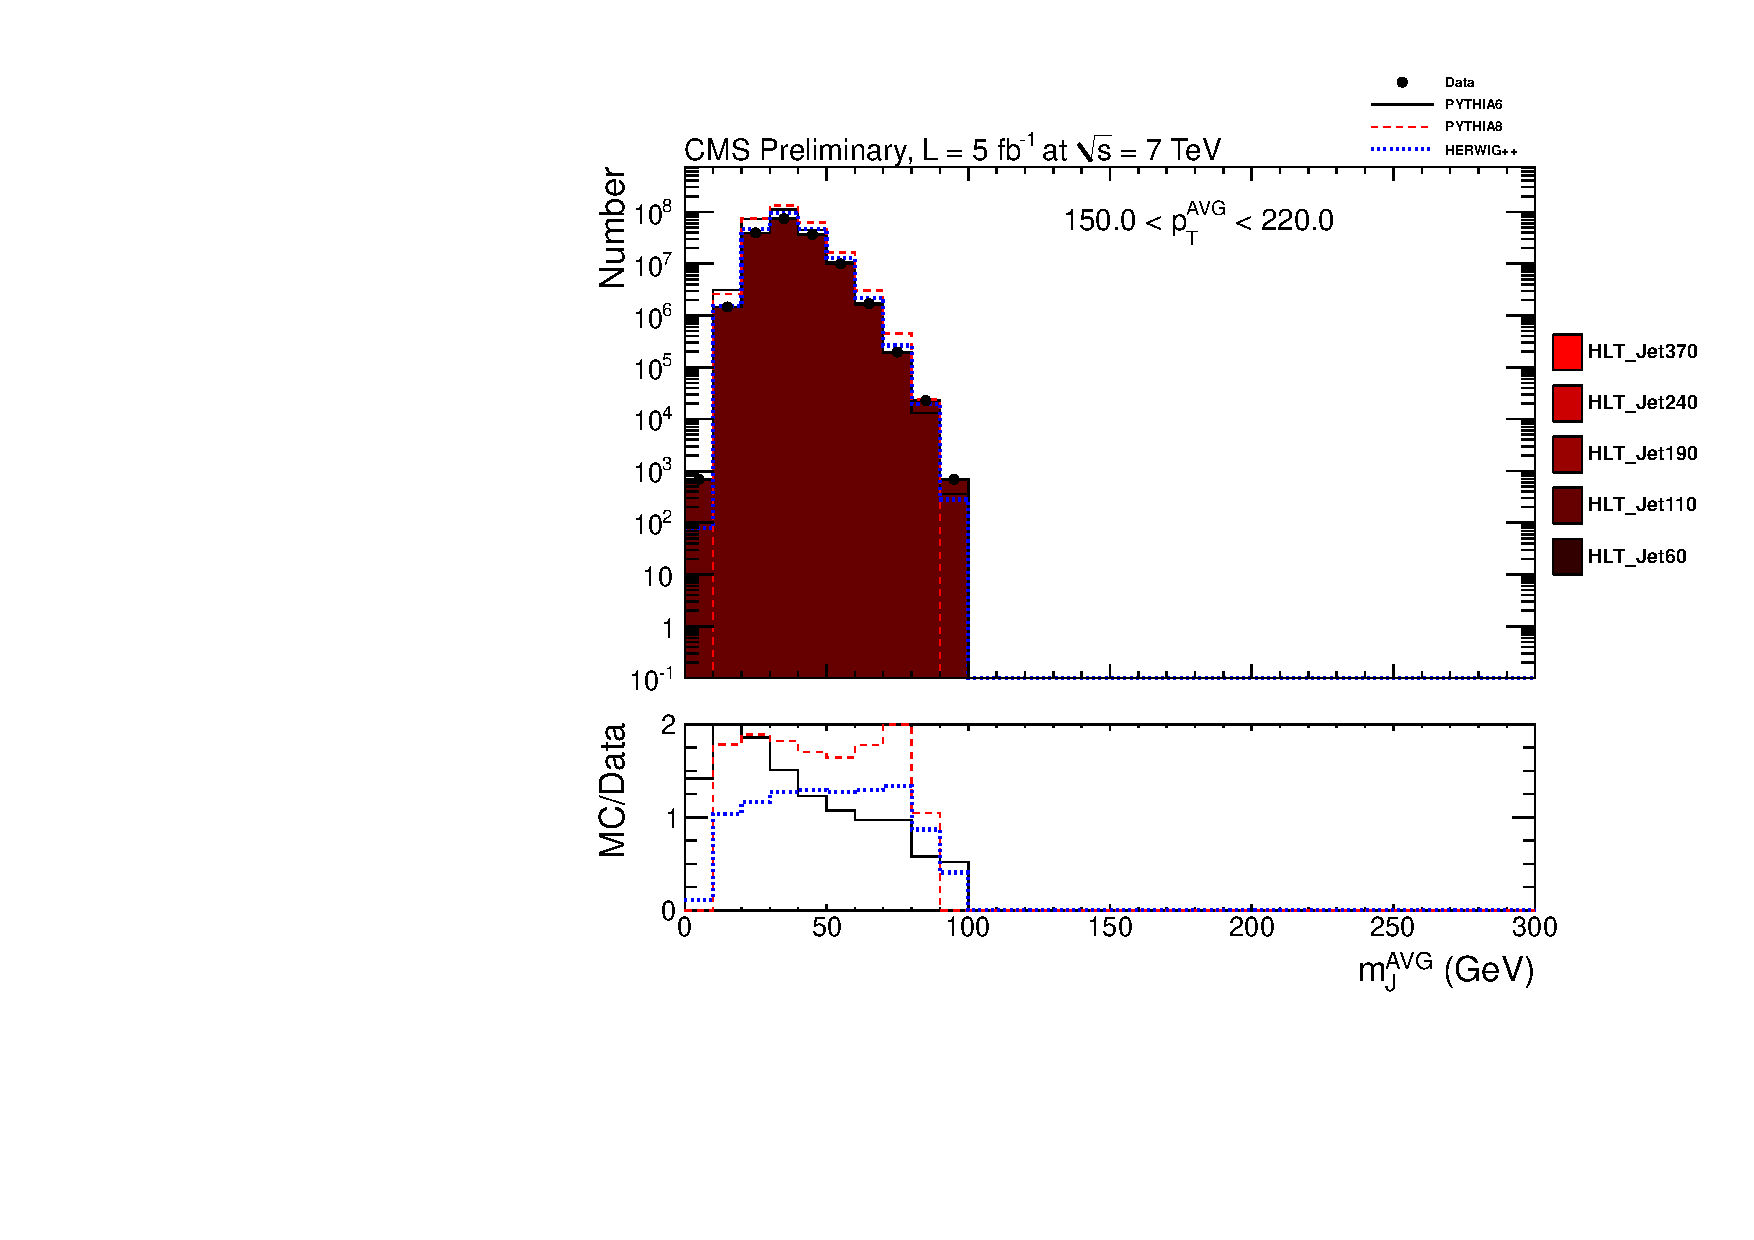
\includegraphics[width=0.95\textwidth]{figs/histAK7MjetVsPtAvg_rawDataMCComparisons_stacktrigs_pt_3}
\caption{Detector-level distributions of the jet mass for AK7 jets,
for $150.0 < \pt^{AVG} < 220.0$ \GeVc. The data are shown in black points.
The simulated distribution from \PYTHIA is shown in solid black, 
the from \PYTHIAEIGHT in dashed red, and from \HERWIG in dotted blue. 
The bottom frame shows the ratio of the simulated distribution
to the distribution from data. The various trigger contributions are shown in shades of red.
\label{figs:histAK7MjetVsPtAvg_rawDataMCComparisons_stacktrigs_pt_3}}
\end{figure}



\begin{figure}[htbp]
\centering
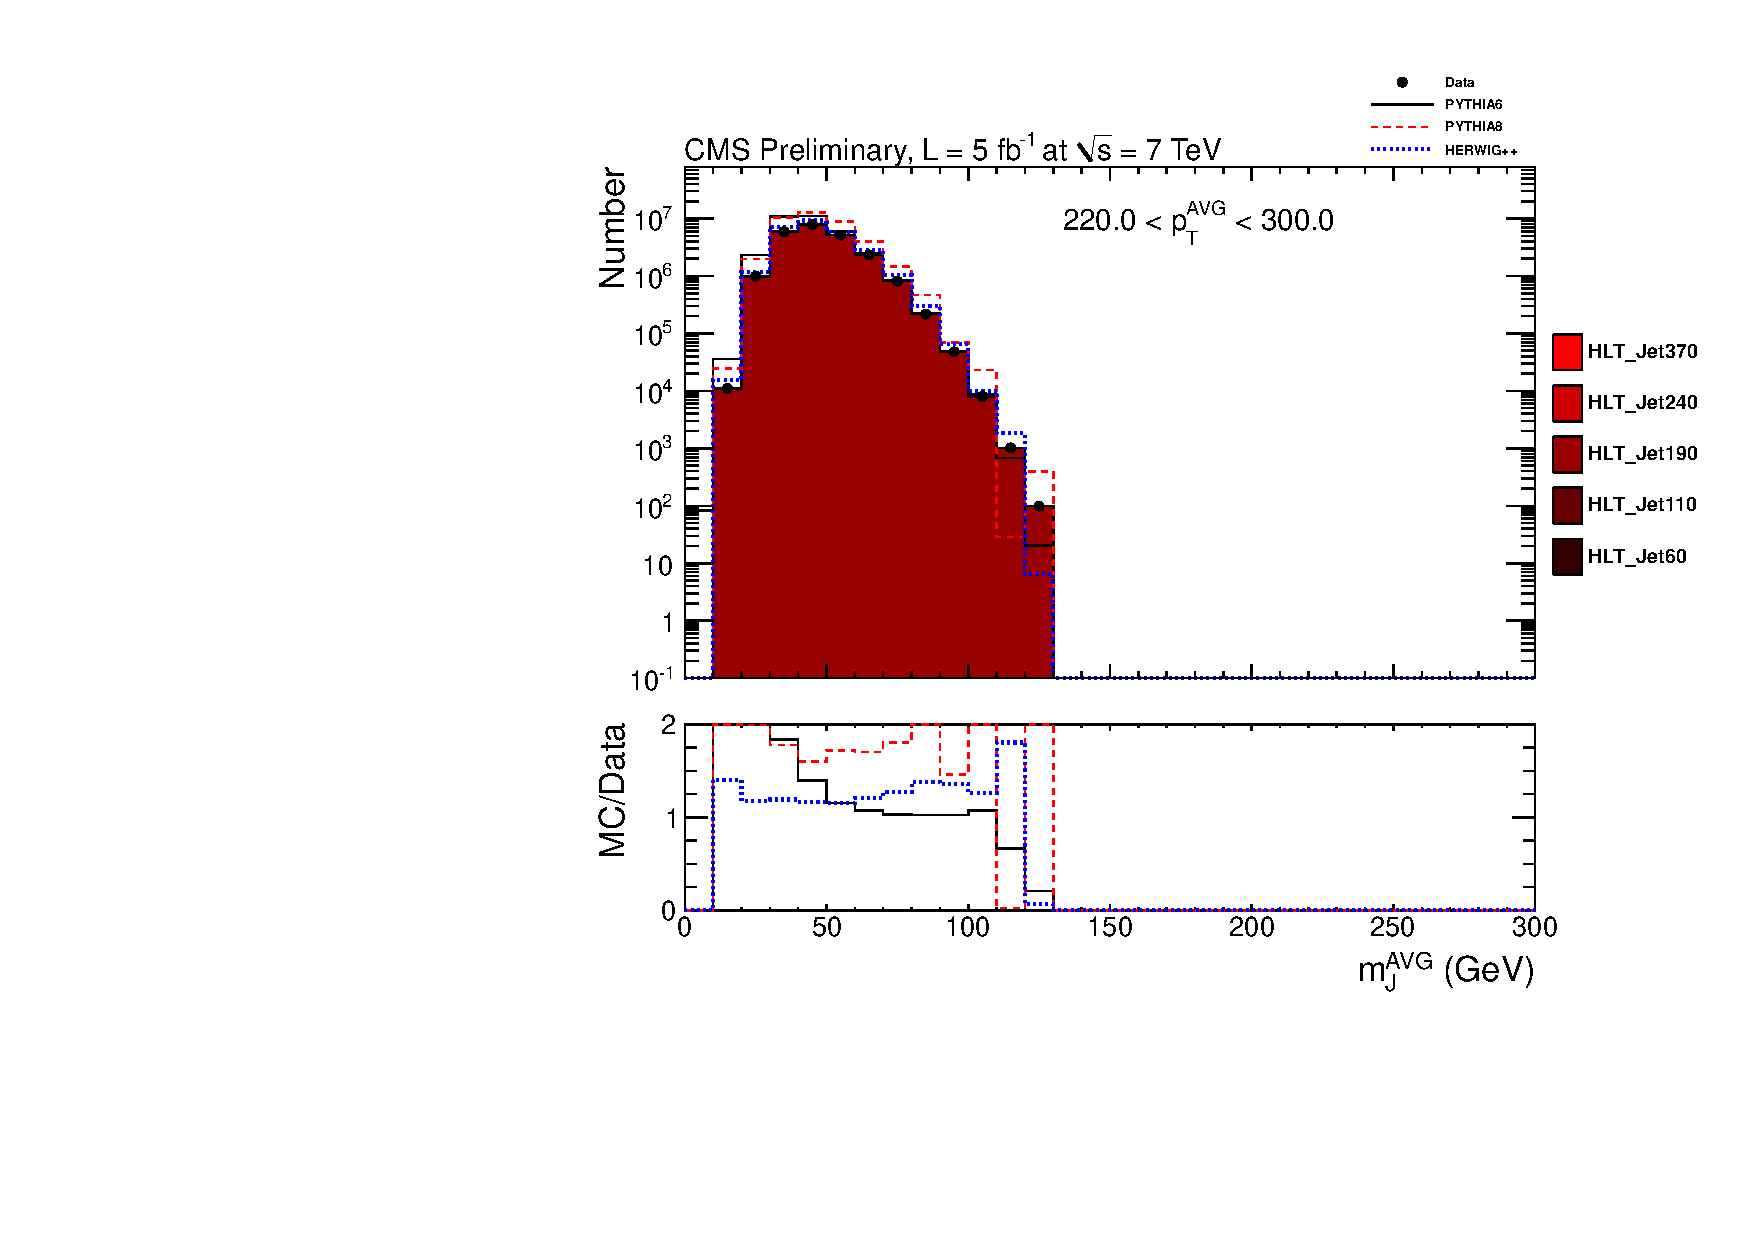
\includegraphics[width=0.95\textwidth]{figs/histAK7MjetVsPtAvg_rawDataMCComparisons_stacktrigs_pt_4}
\caption{Detector-level distributions of the jet mass for AK7 jets,
for $220.0 < \pt^{AVG} < 300.0$ \GeVc. The data are shown in black points.
The simulated distribution from \PYTHIA is shown in solid black, 
the from \PYTHIAEIGHT in dashed red, and from \HERWIG in dotted blue. 
The bottom frame shows the ratio of the simulated distribution
to the distribution from data. The various trigger contributions are shown in shades of red.
\label{figs:histAK7MjetVsPtAvg_rawDataMCComparisons_stacktrigs_pt_4}}
\end{figure}



\begin{figure}[htbp]
\centering
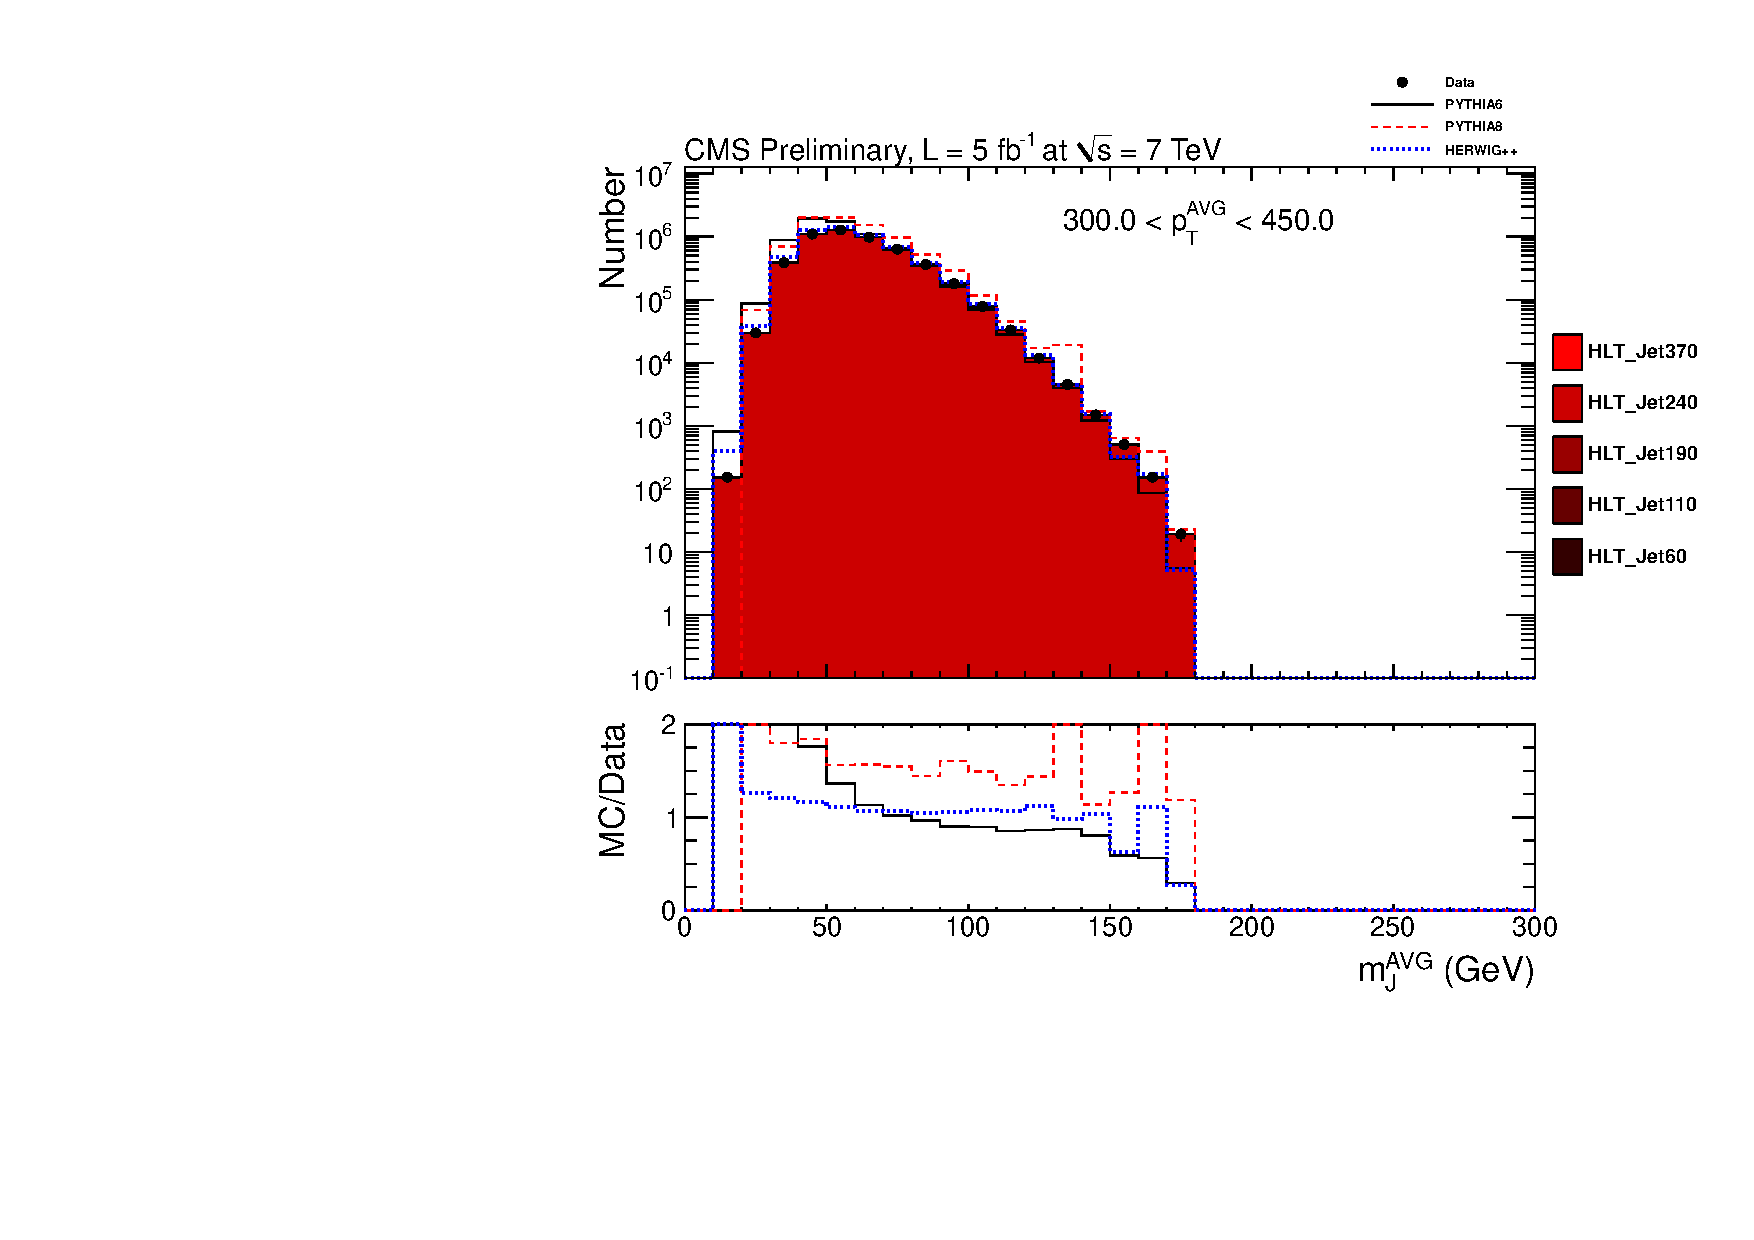
\includegraphics[width=0.95\textwidth]{figs/histAK7MjetVsPtAvg_rawDataMCComparisons_stacktrigs_pt_5}
\caption{Detector-level distributions of the jet mass for AK7 jets,
for $300.0 < \pt^{AVG} < 450.0$ \GeVc. The data are shown in black points.
The simulated distribution from \PYTHIA is shown in solid black, 
the from \PYTHIAEIGHT in dashed red, and from \HERWIG in dotted blue. 
The bottom frame shows the ratio of the simulated distribution
to the distribution from data. The various trigger contributions are shown in shades of red.
\label{figs:histAK7MjetVsPtAvg_rawDataMCComparisons_stacktrigs_pt_5}}
\end{figure}



\begin{figure}[htbp]
\centering
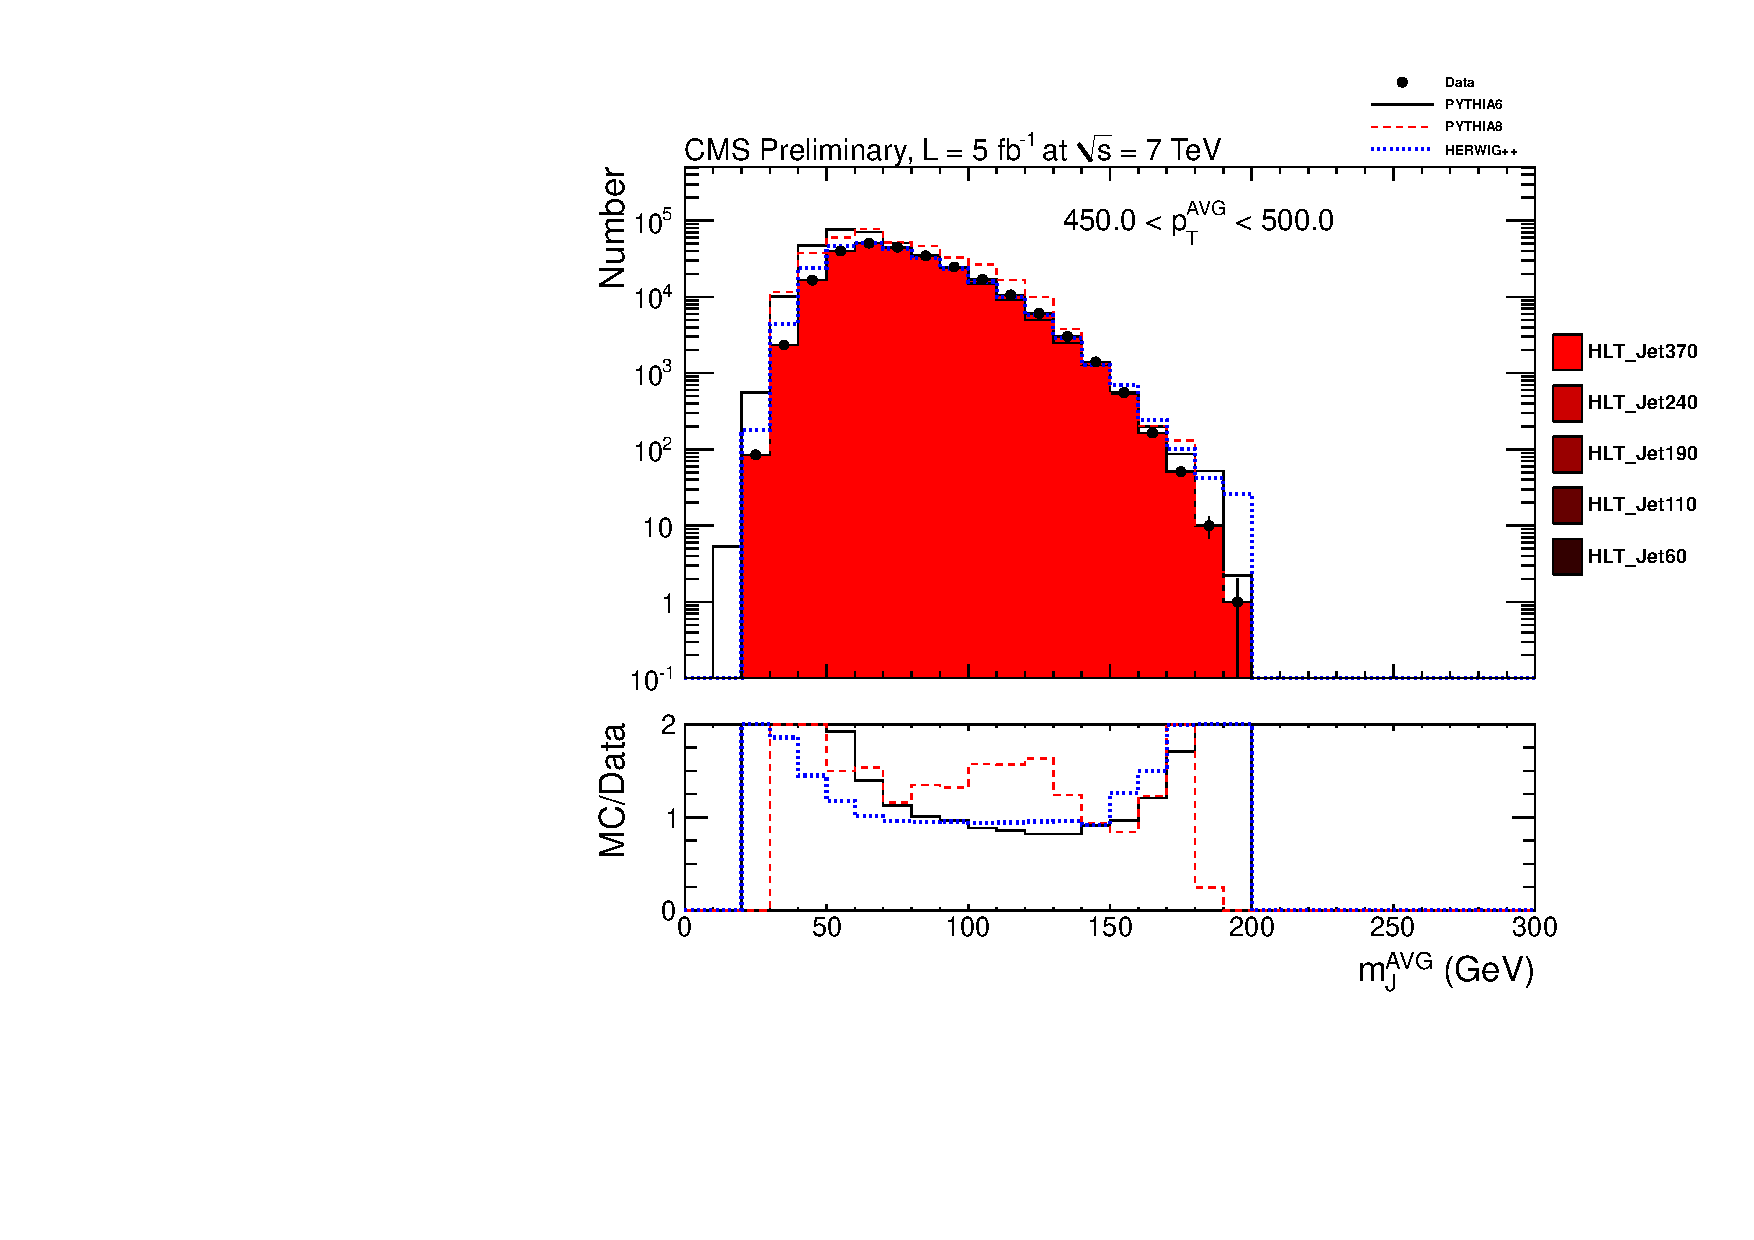
\includegraphics[width=0.95\textwidth]{figs/histAK7MjetVsPtAvg_rawDataMCComparisons_stacktrigs_pt_6}
\caption{Detector-level distributions of the jet mass for AK7 jets,
for $450.0 < \pt^{AVG} < 500.0$ \GeVc. The data are shown in black points.
The simulated distribution from \PYTHIA is shown in solid black, 
the from \PYTHIAEIGHT in dashed red, and from \HERWIG in dotted blue. 
The bottom frame shows the ratio of the simulated distribution
to the distribution from data. The various trigger contributions are shown in shades of red.
\label{figs:histAK7MjetVsPtAvg_rawDataMCComparisons_stacktrigs_pt_6}}
\end{figure}



\begin{figure}[htbp]
\centering
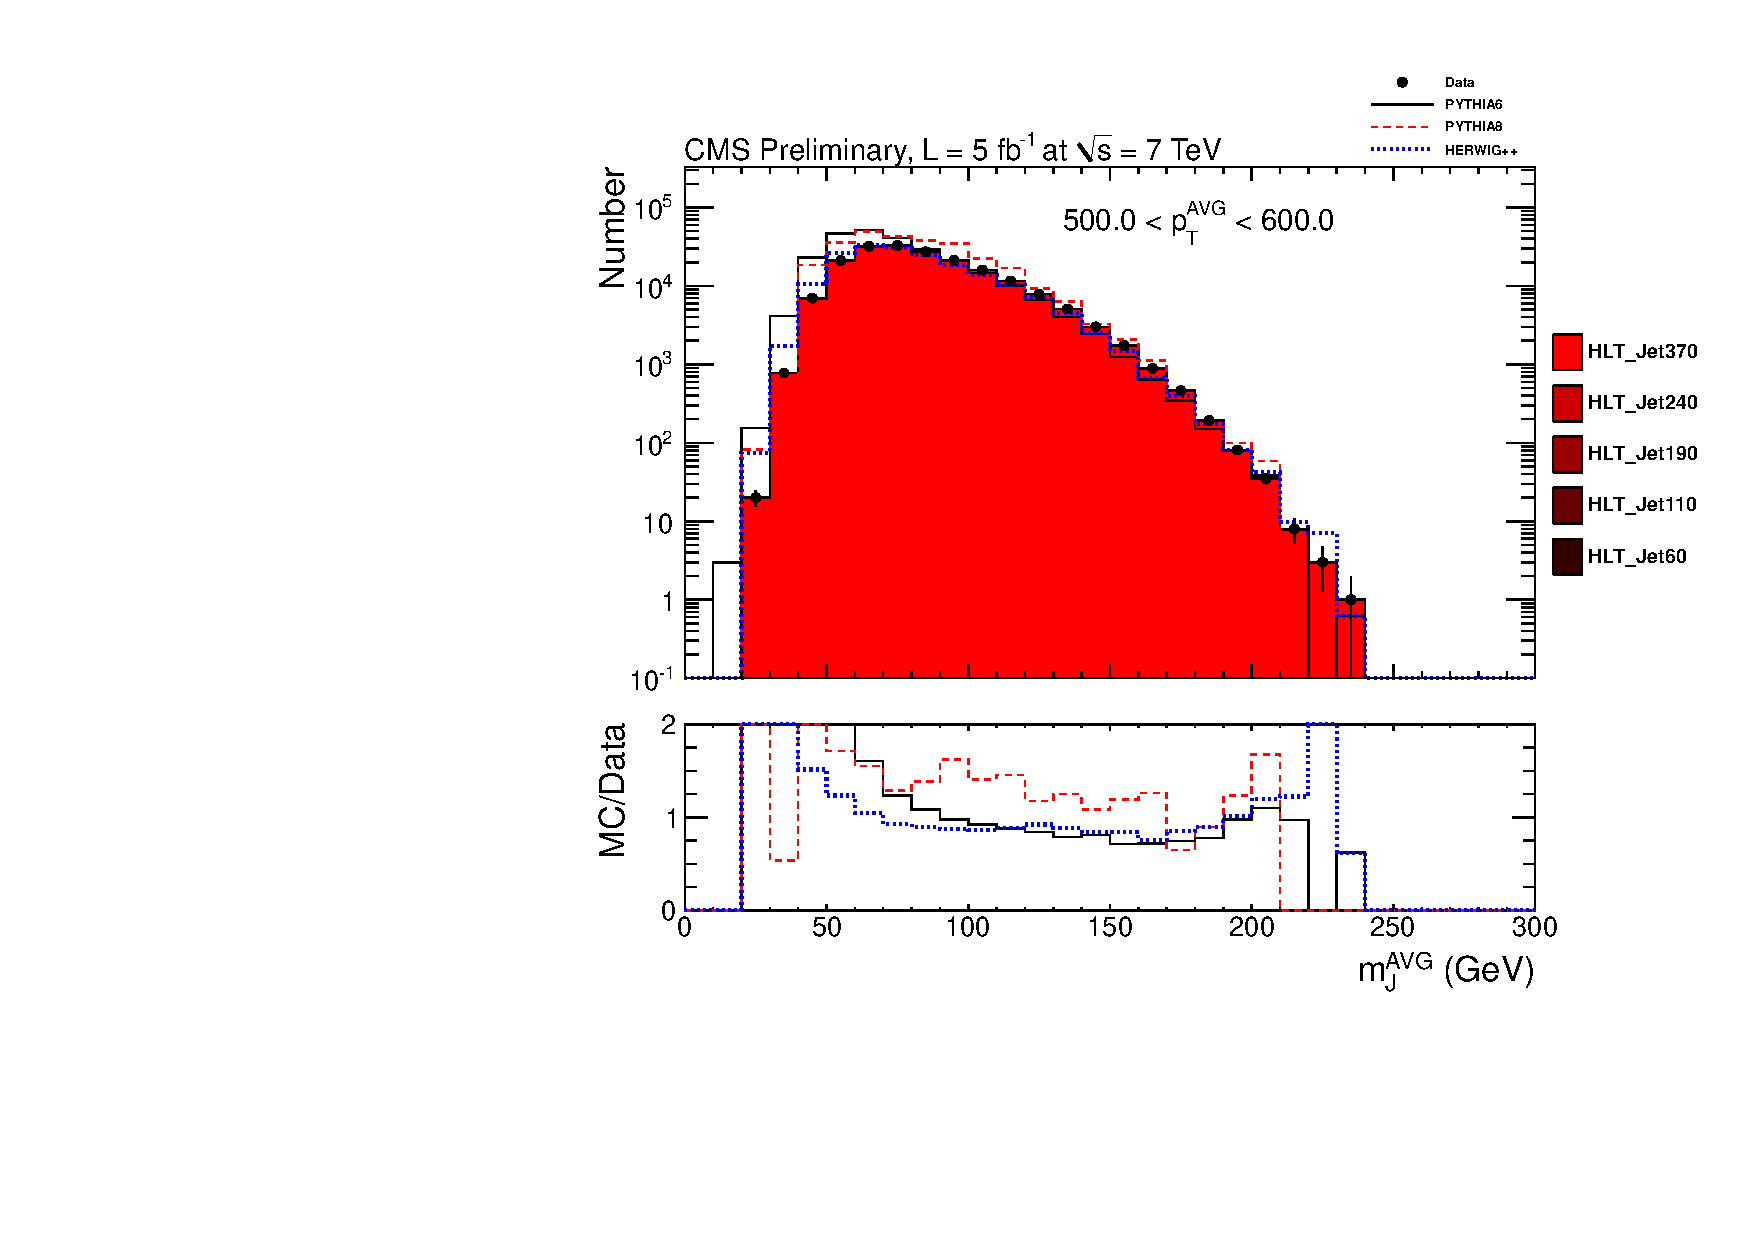
\includegraphics[width=0.95\textwidth]{figs/histAK7MjetVsPtAvg_rawDataMCComparisons_stacktrigs_pt_7}
\caption{Detector-level distributions of the jet mass for AK7 jets,
for $500.0 < \pt^{AVG} < 600.0$ \GeVc. The data are shown in black points.
The simulated distribution from \PYTHIA is shown in solid black, 
the from \PYTHIAEIGHT in dashed red, and from \HERWIG in dotted blue. 
The bottom frame shows the ratio of the simulated distribution
to the distribution from data. The various trigger contributions are shown in shades of red.
\label{figs:histAK7MjetVsPtAvg_rawDataMCComparisons_stacktrigs_pt_7}}
\end{figure}



\begin{figure}[htbp]
\centering
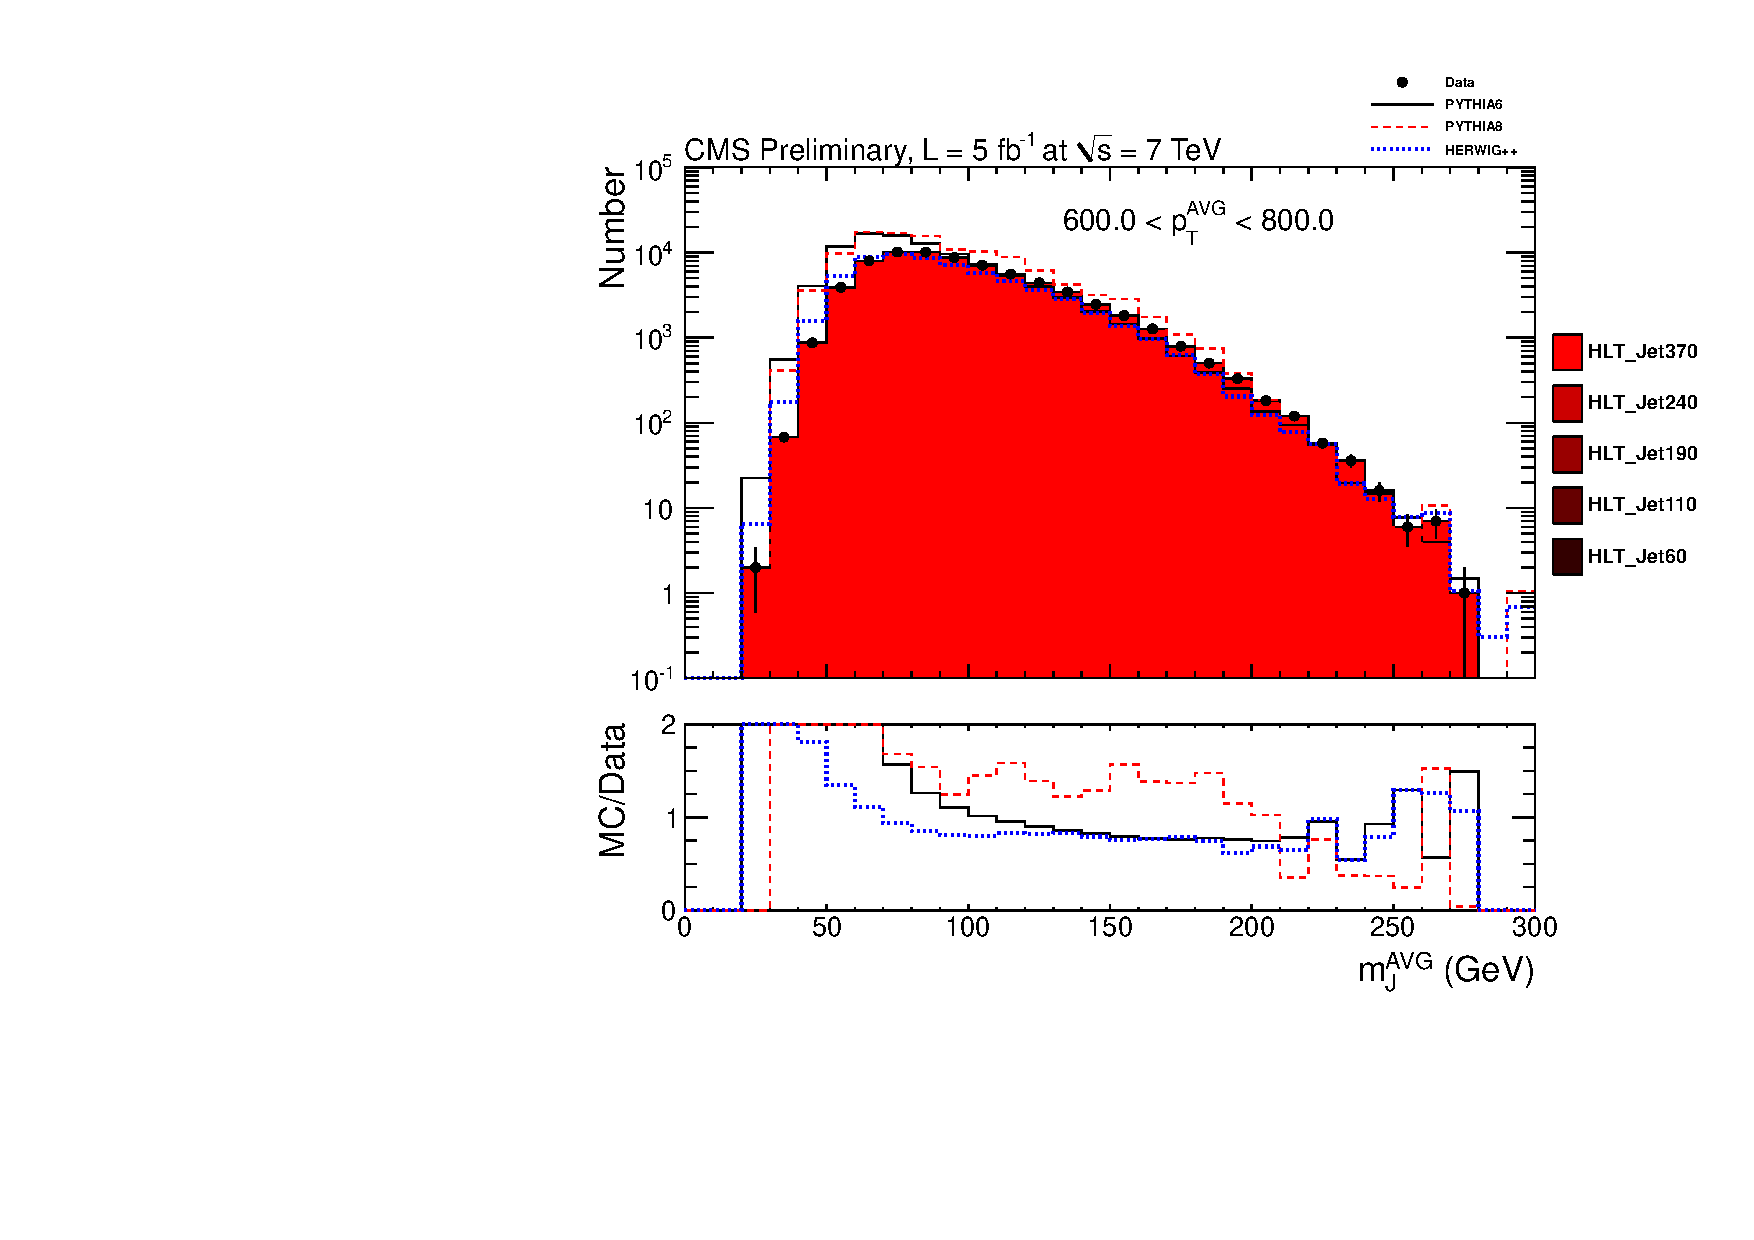
\includegraphics[width=0.95\textwidth]{figs/histAK7MjetVsPtAvg_rawDataMCComparisons_stacktrigs_pt_8}
\caption{Detector-level distributions of the jet mass for AK7 jets,
for $600.0 < \pt^{AVG} < 800.0$ \GeVc. The data are shown in black points.
The simulated distribution from \PYTHIA is shown in solid black, 
the from \PYTHIAEIGHT in dashed red, and from \HERWIG in dotted blue. 
The bottom frame shows the ratio of the simulated distribution
to the distribution from data. The various trigger contributions are shown in shades of red.
\label{figs:histAK7MjetVsPtAvg_rawDataMCComparisons_stacktrigs_pt_8}}
\end{figure}



\begin{figure}[htbp]
\centering
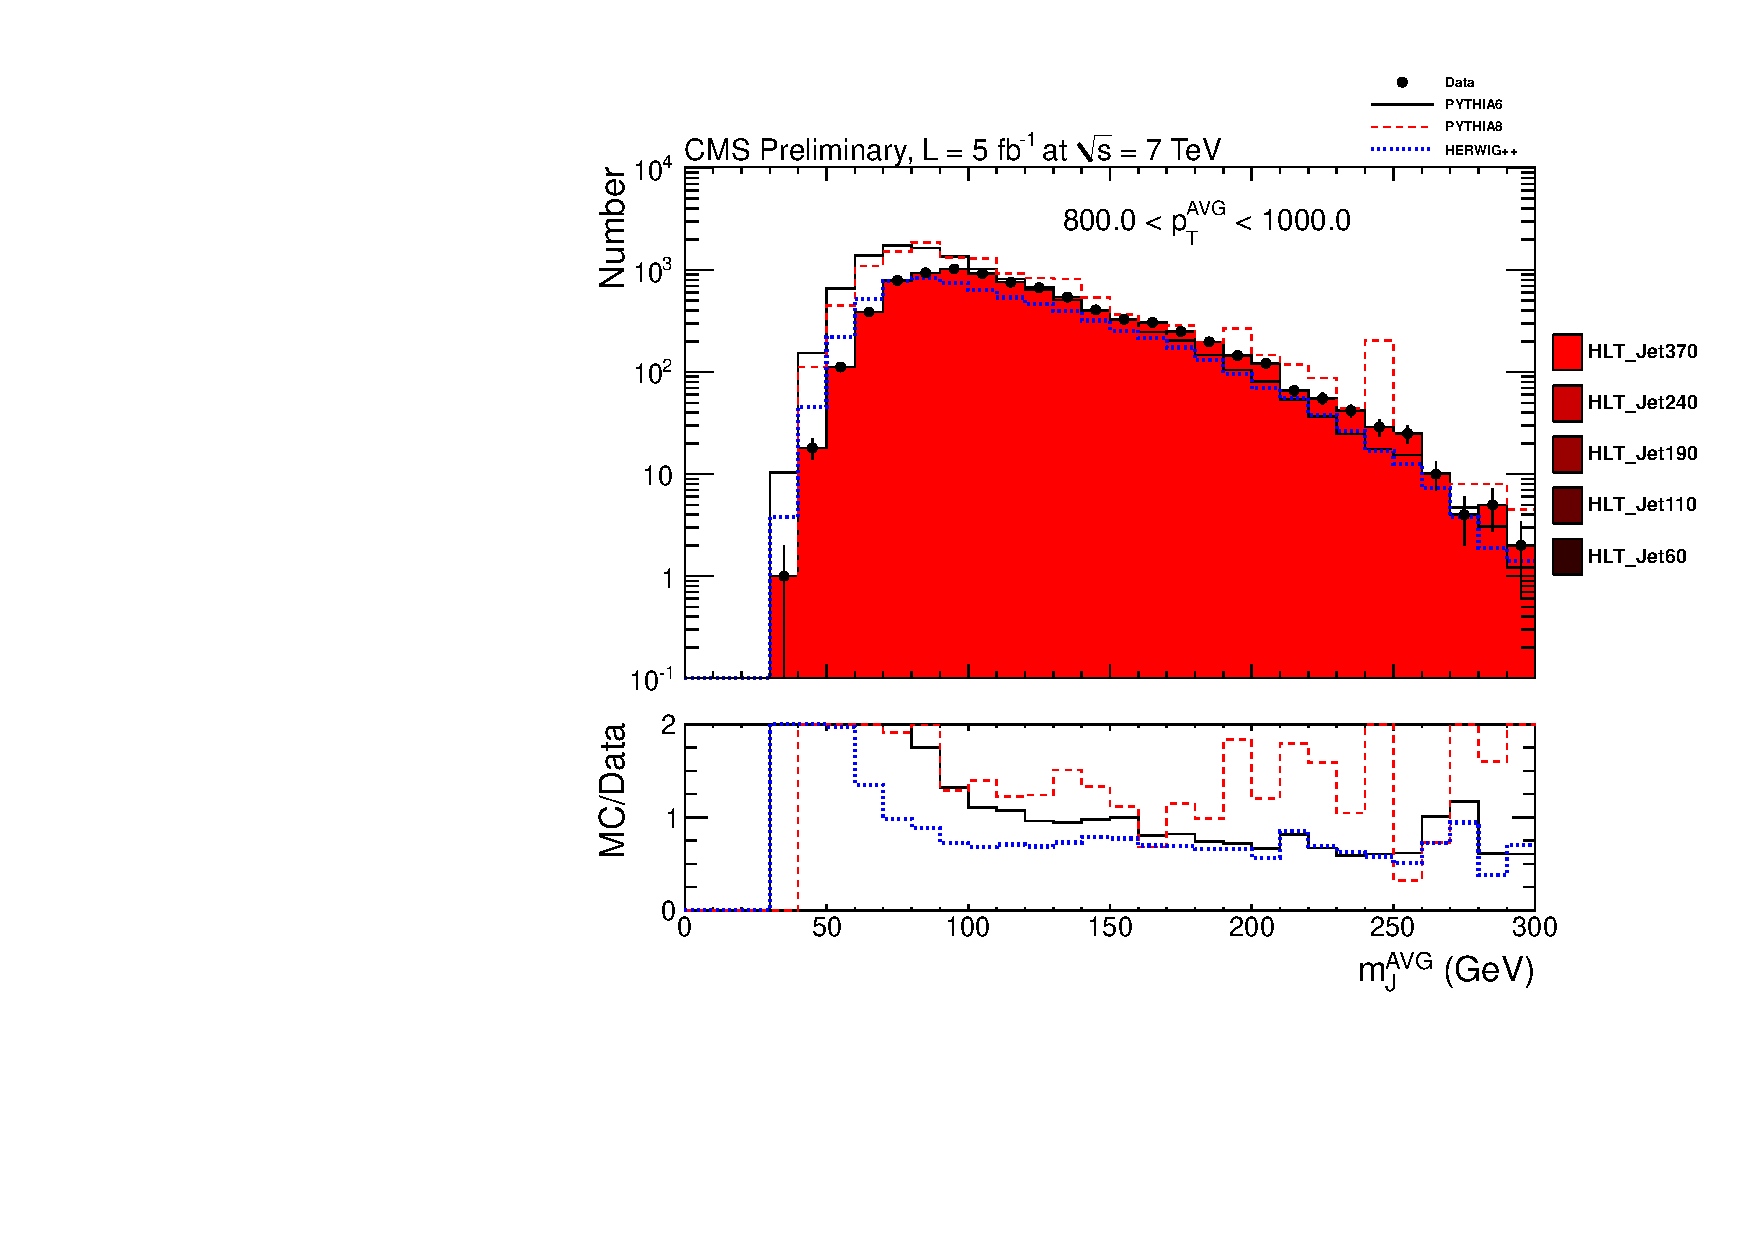
\includegraphics[width=0.95\textwidth]{figs/histAK7MjetVsPtAvg_rawDataMCComparisons_stacktrigs_pt_9}
\caption{Detector-level distributions of the jet mass for AK7 jets,
for $800.0 < \pt^{AVG} < 1000.0$ \GeVc. The data are shown in black points.
The simulated distribution from \PYTHIA is shown in solid black, 
the from \PYTHIAEIGHT in dashed red, and from \HERWIG in dotted blue. 
The bottom frame shows the ratio of the simulated distribution
to the distribution from data. The various trigger contributions are shown in shades of red.
\label{figs:histAK7MjetVsPtAvg_rawDataMCComparisons_stacktrigs_pt_9}}
\end{figure}



\begin{figure}[htbp]
\centering
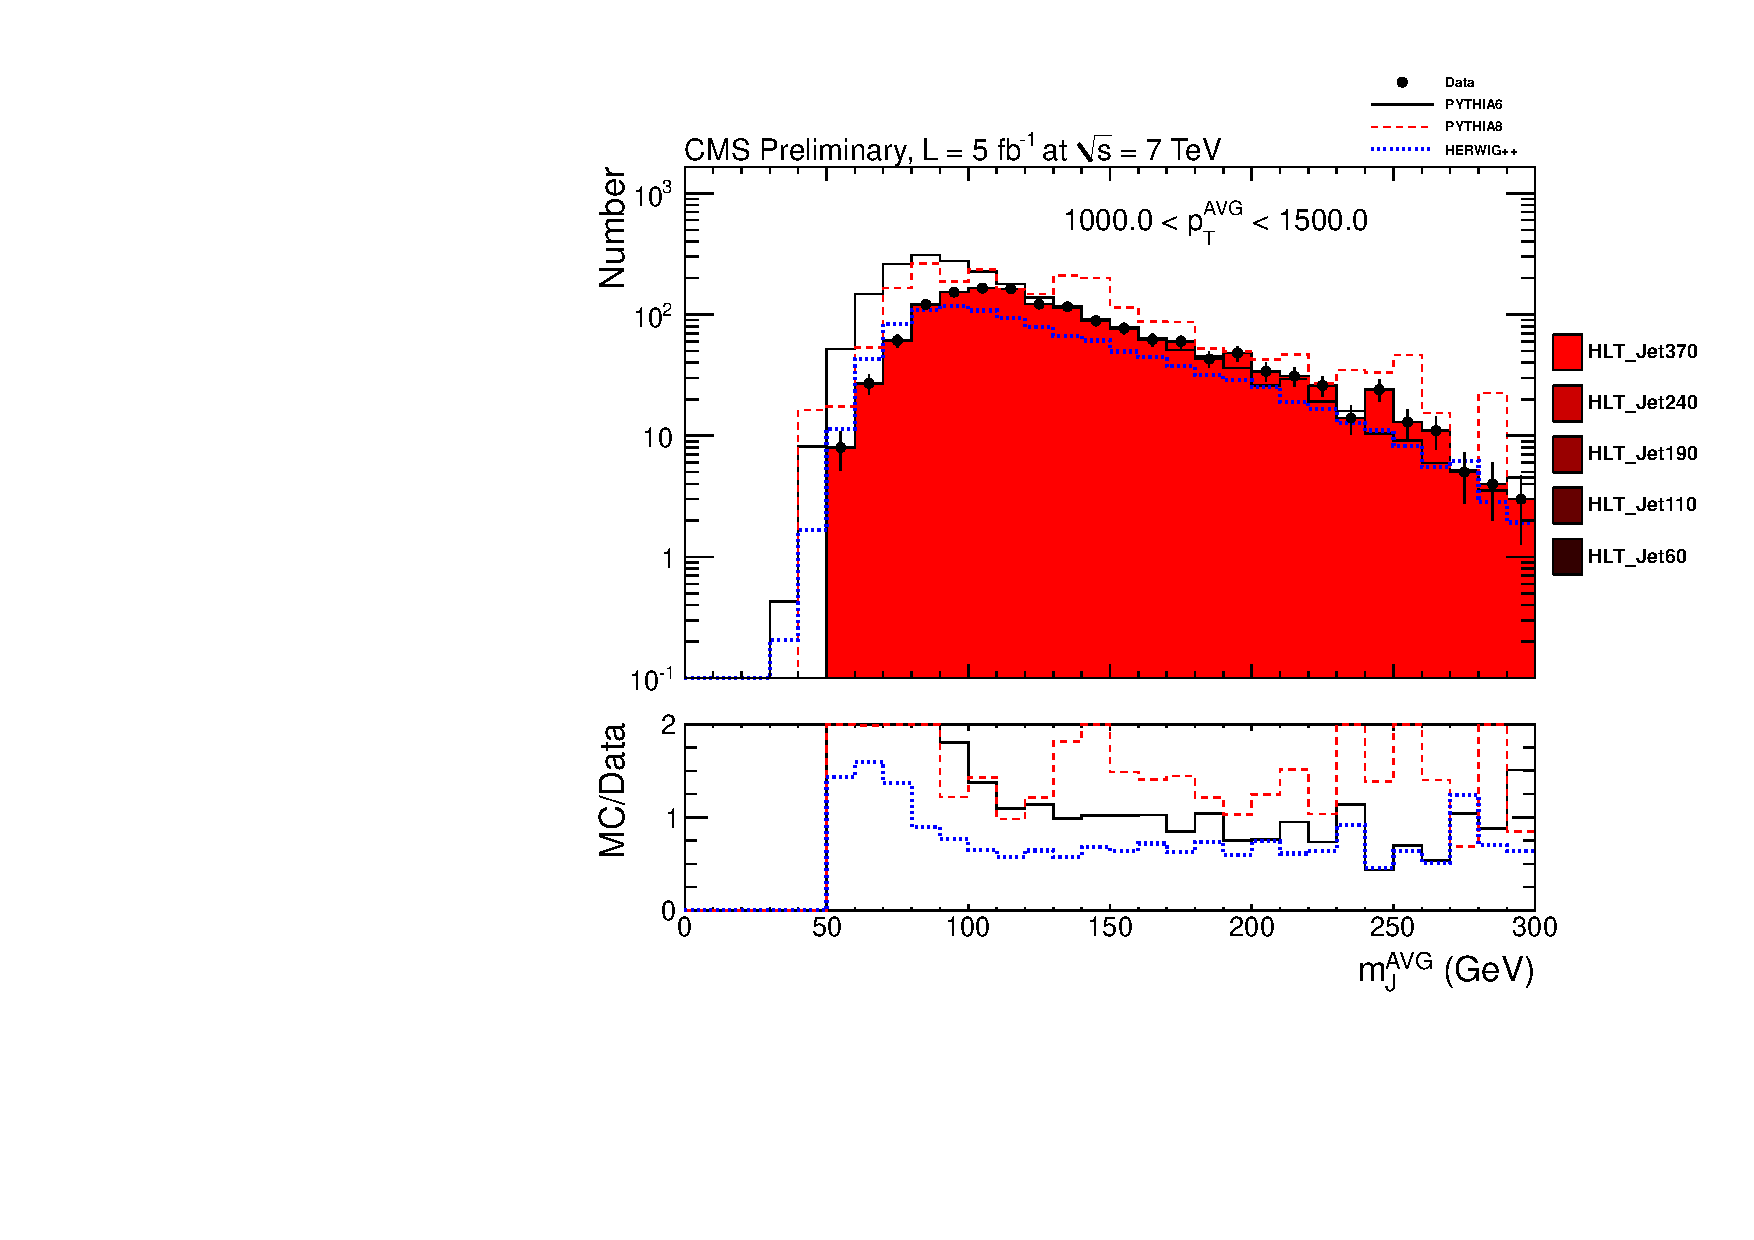
\includegraphics[width=0.95\textwidth]{figs/histAK7MjetVsPtAvg_rawDataMCComparisons_stacktrigs_pt_10}
\caption{Detector-level distributions of the jet mass for AK7 jets,
for $1000.0 < \pt^{AVG} < 1500.0$ \GeVc. The data are shown in black points.
The simulated distribution from \PYTHIA is shown in solid black, 
the from \PYTHIAEIGHT in dashed red, and from \HERWIG in dotted blue. 
The bottom frame shows the ratio of the simulated distribution
to the distribution from data. The various trigger contributions are shown in shades of red.
\label{figs:histAK7MjetVsPtAvg_rawDataMCComparisons_stacktrigs_pt_10}}
\end{figure}

\clearpage



\begin{figure}[htbp]
\centering
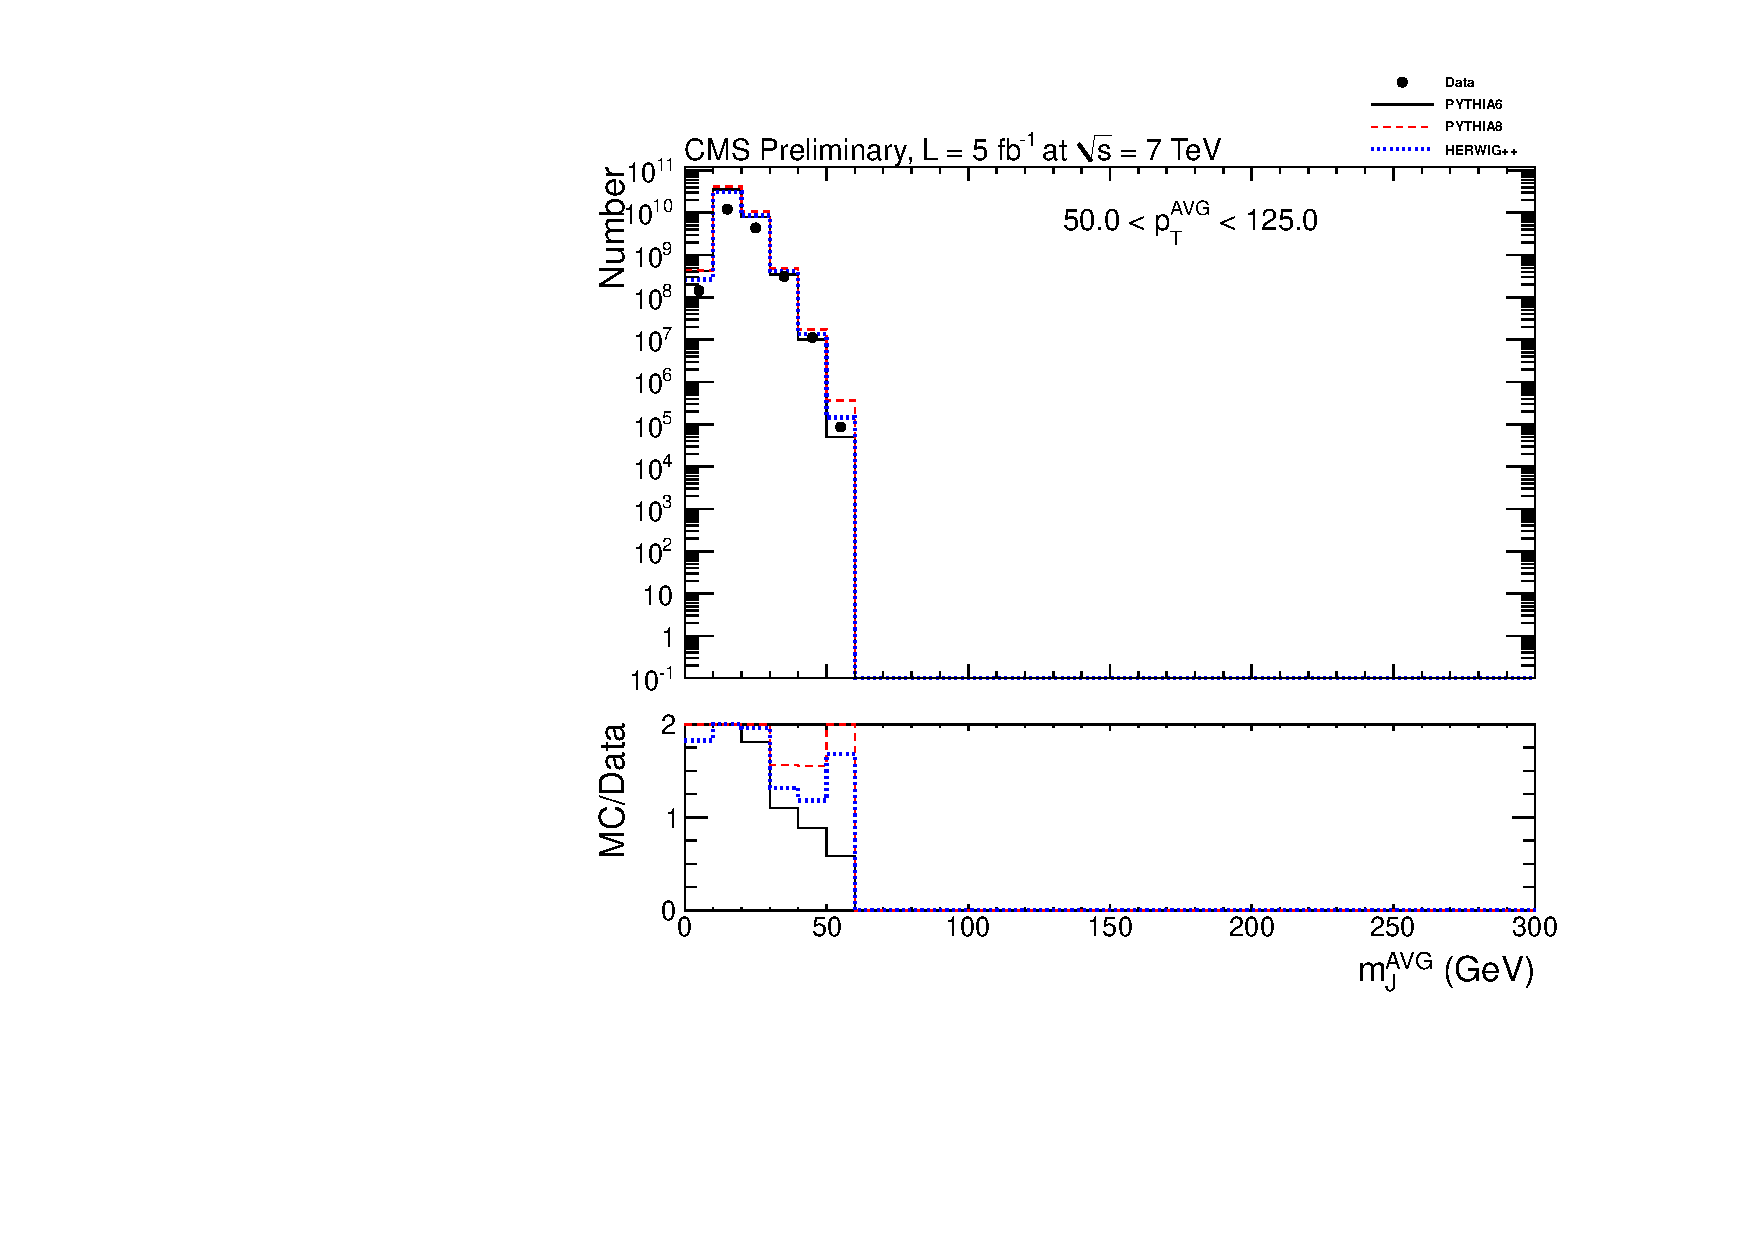
\includegraphics[width=0.95\textwidth]{figs/histAK7MjetVsPtAvg_rawDataMCComparisons_pt_1}
\caption{Detector-level distributions of the jet mass for AK7 jets,
for $50.0 < \pt^{AVG} < 125.0$ \GeVc. The data are shown in black points.
The simulated distribution from \PYTHIA is shown in solid black, 
the from \PYTHIAEIGHT in dashed red, and from \HERWIG in dotted blue. 
The bottom frame shows the ratio of the simulated distribution
to the distribution from data. 
\label{figs:histAK7MjetVsPtAvg_rawDataMCComparisons_pt_1}}
\end{figure}



\begin{figure}[htbp]
\centering
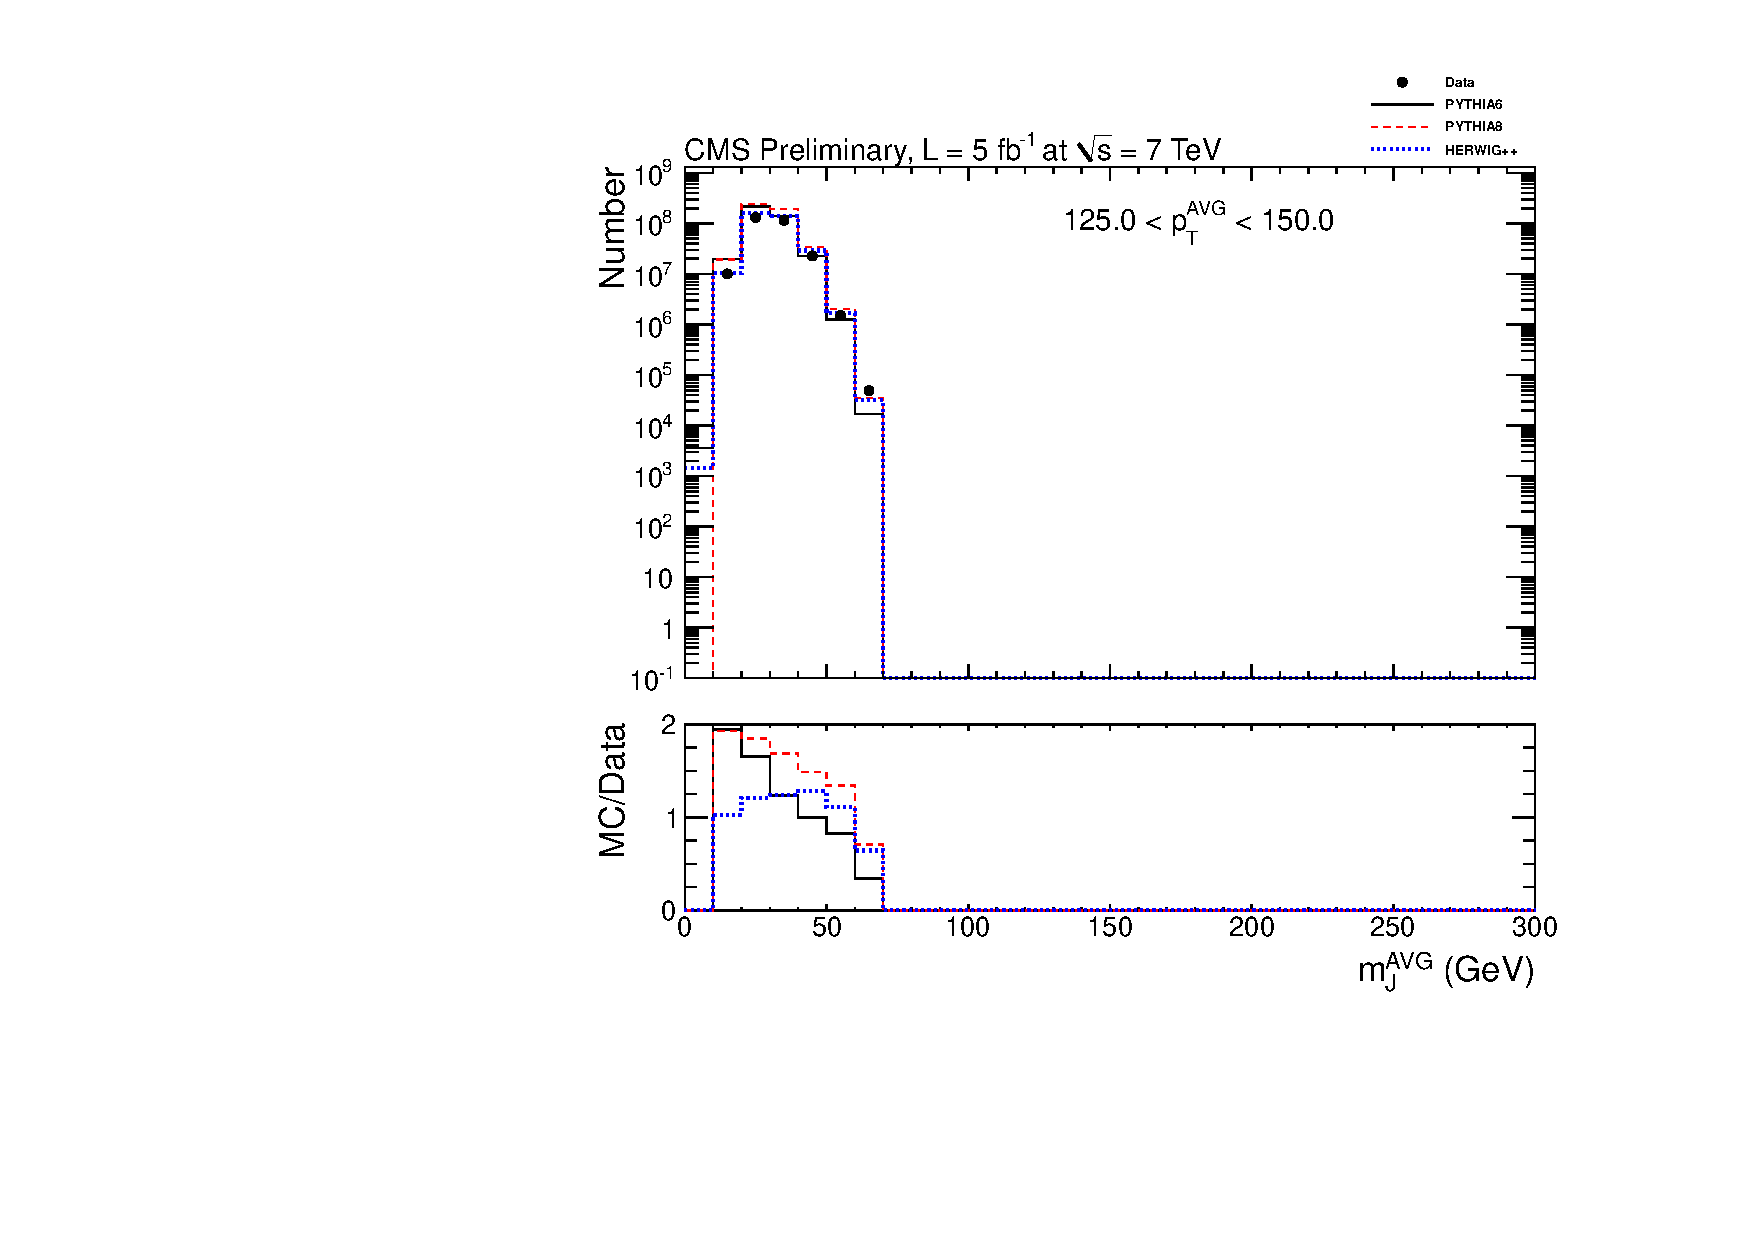
\includegraphics[width=0.95\textwidth]{figs/histAK7MjetVsPtAvg_rawDataMCComparisons_pt_2}
\caption{Detector-level distributions of the jet mass for AK7 jets,
for $125.0 < \pt^{AVG} < 150.0$ \GeVc. The data are shown in black points.
The simulated distribution from \PYTHIA is shown in solid black, 
the from \PYTHIAEIGHT in dashed red, and from \HERWIG in dotted blue. 
The bottom frame shows the ratio of the simulated distribution
to the distribution from data. 
\label{figs:histAK7MjetVsPtAvg_rawDataMCComparisons_pt_2}}
\end{figure}



\begin{figure}[htbp]
\centering
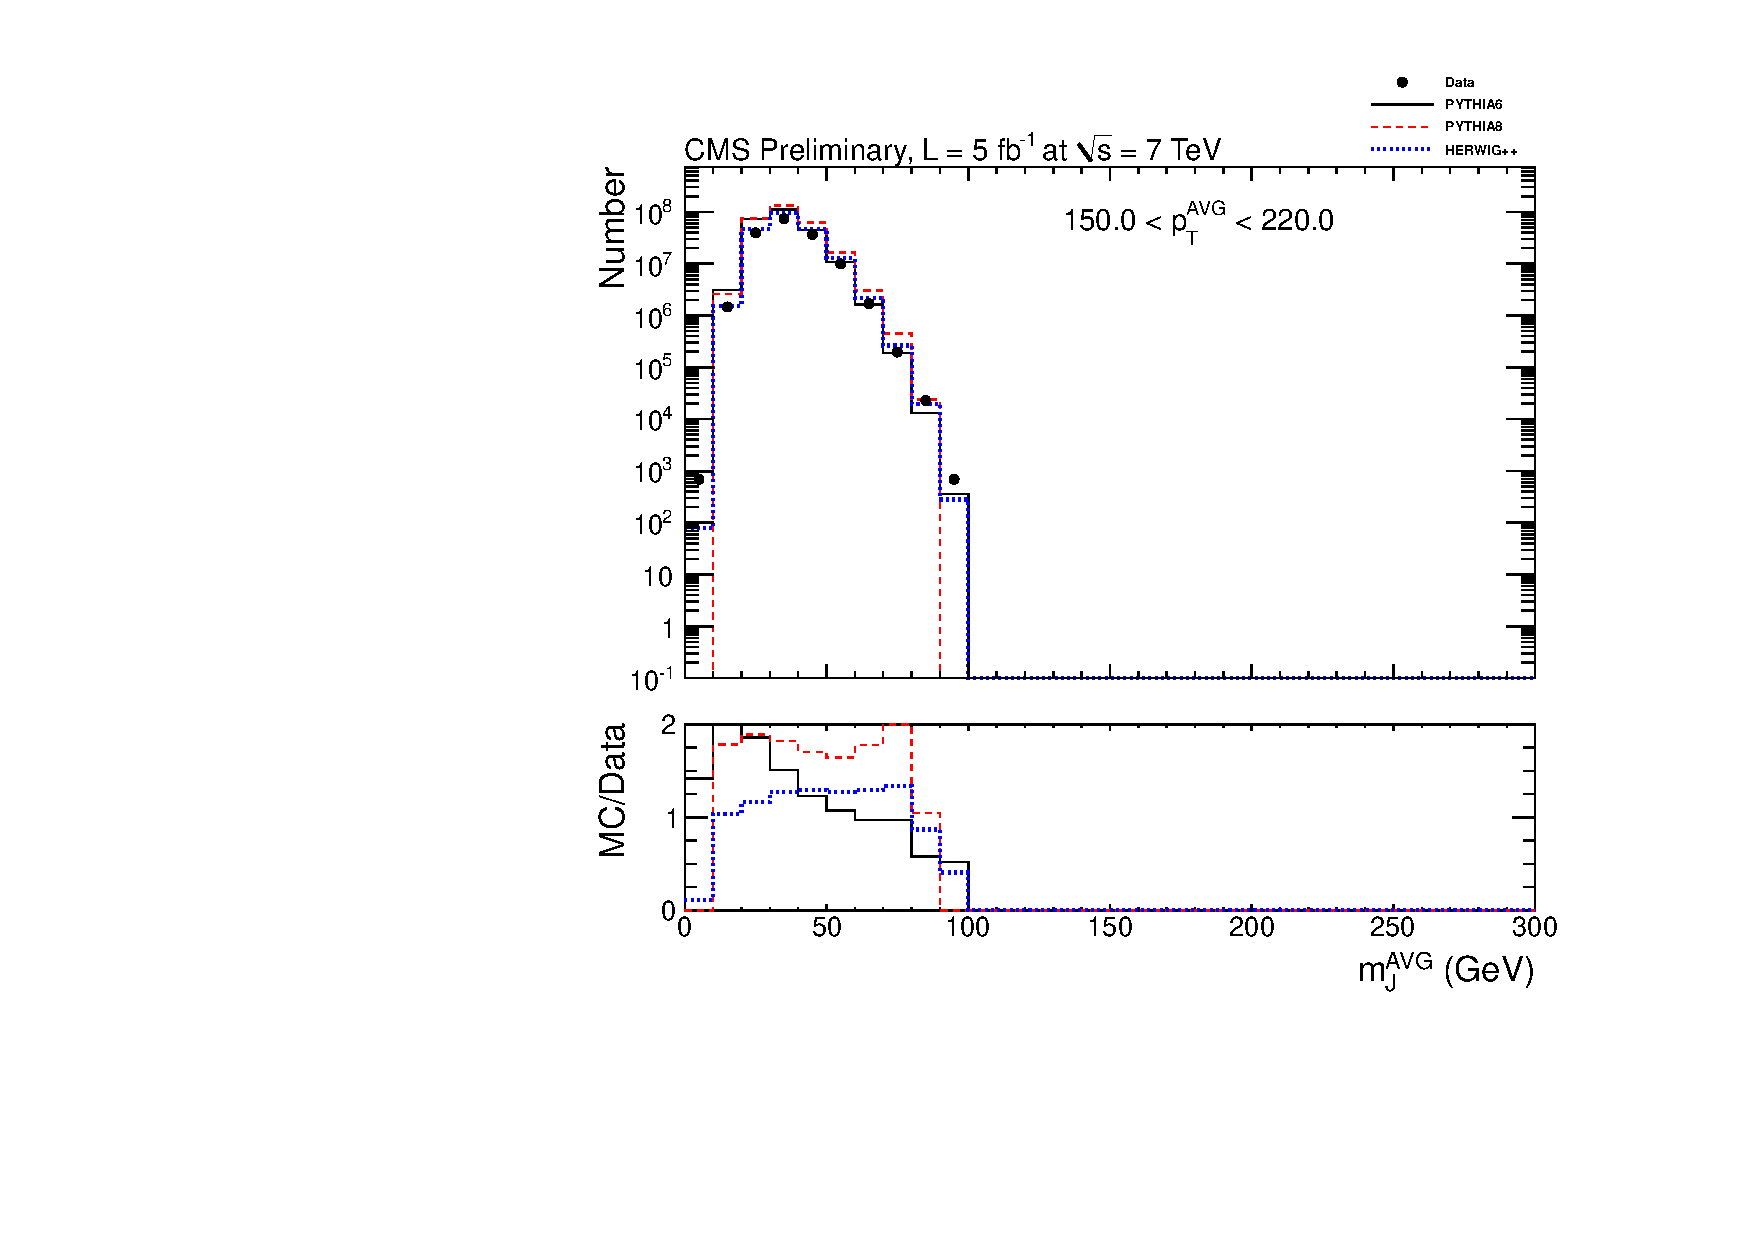
\includegraphics[width=0.95\textwidth]{figs/histAK7MjetVsPtAvg_rawDataMCComparisons_pt_3}
\caption{Detector-level distributions of the jet mass for AK7 jets,
for $150.0 < \pt^{AVG} < 220.0$ \GeVc. The data are shown in black points.
The simulated distribution from \PYTHIA is shown in solid black, 
the from \PYTHIAEIGHT in dashed red, and from \HERWIG in dotted blue. 
The bottom frame shows the ratio of the simulated distribution
to the distribution from data. 
\label{figs:histAK7MjetVsPtAvg_rawDataMCComparisons_pt_3}}
\end{figure}



\begin{figure}[htbp]
\centering
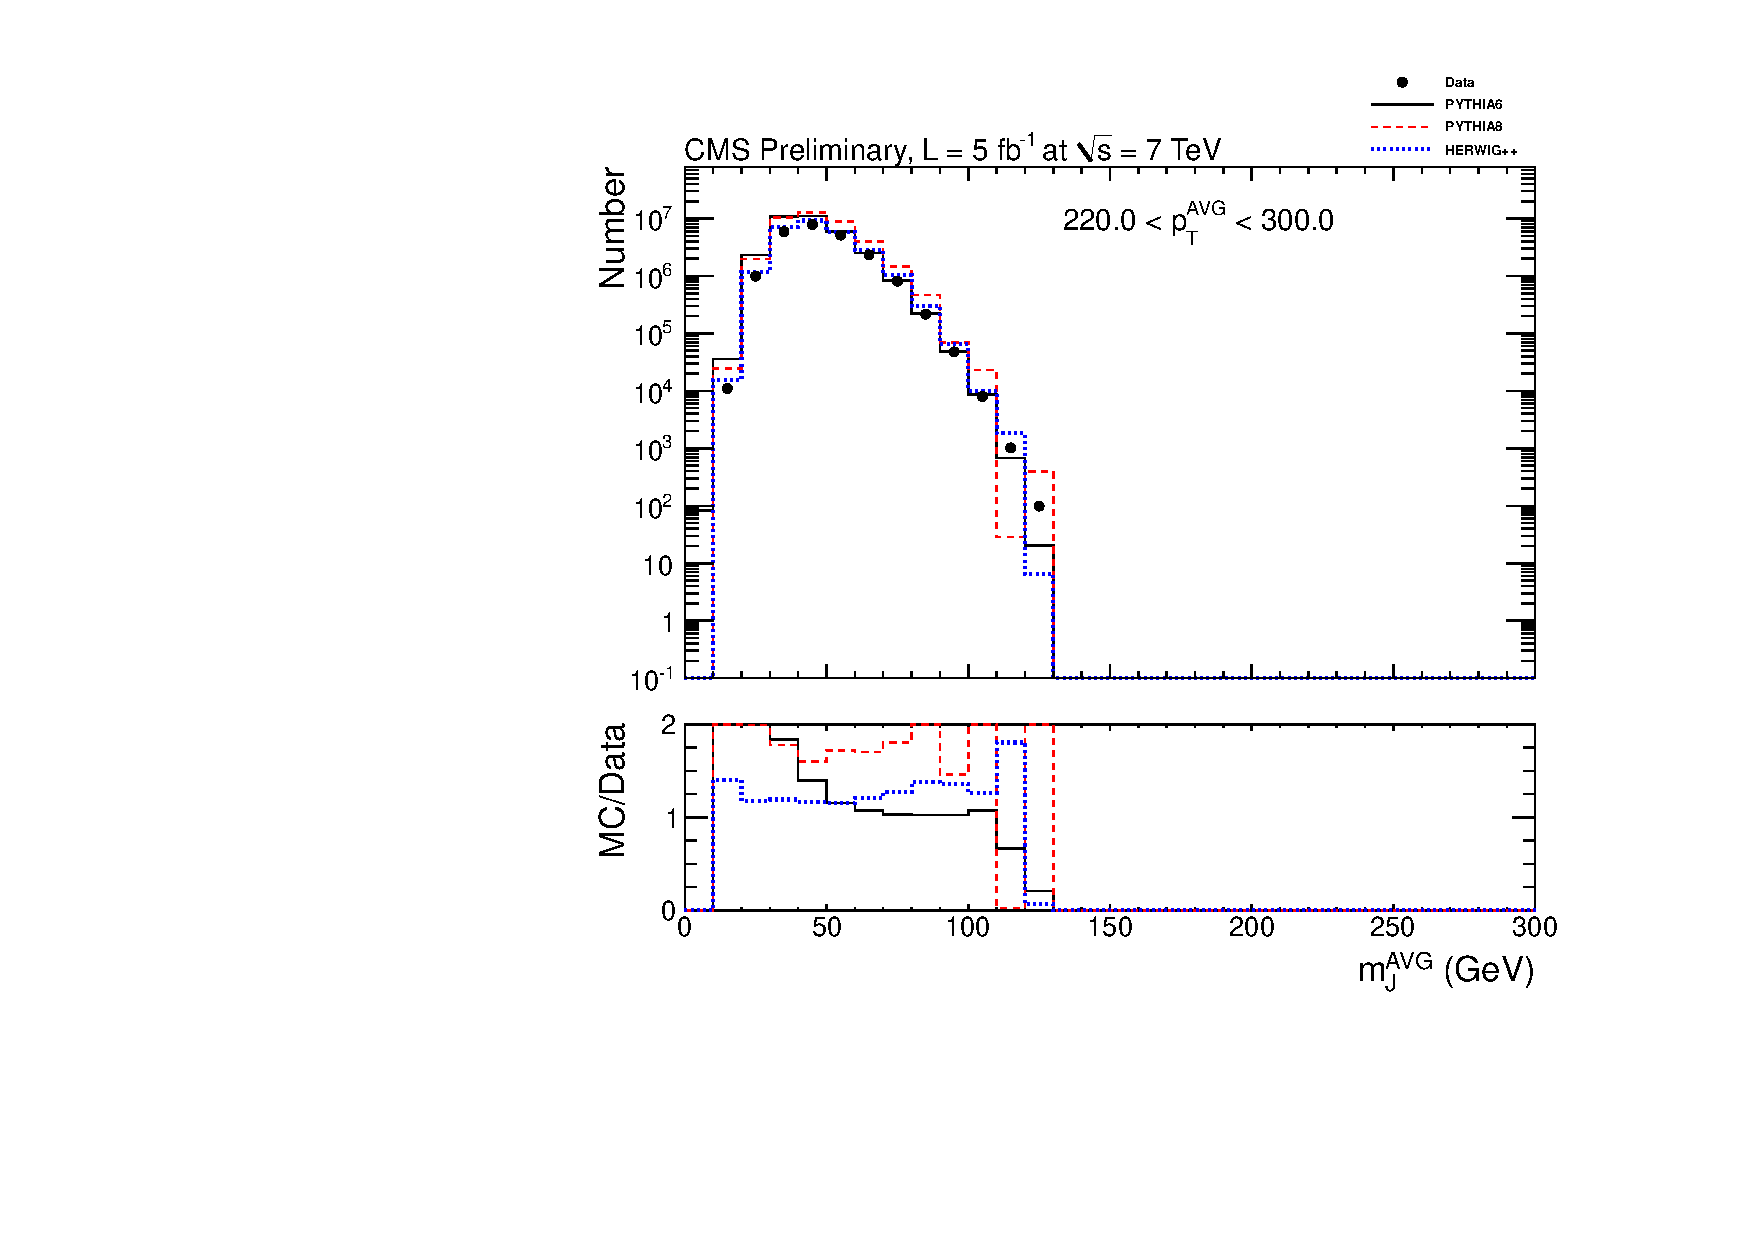
\includegraphics[width=0.95\textwidth]{figs/histAK7MjetVsPtAvg_rawDataMCComparisons_pt_4}
\caption{Detector-level distributions of the jet mass for AK7 jets,
for $220.0 < \pt^{AVG} < 300.0$ \GeVc. The data are shown in black points.
The simulated distribution from \PYTHIA is shown in solid black, 
the from \PYTHIAEIGHT in dashed red, and from \HERWIG in dotted blue. 
The bottom frame shows the ratio of the simulated distribution
to the distribution from data. 
\label{figs:histAK7MjetVsPtAvg_rawDataMCComparisons_pt_4}}
\end{figure}



\begin{figure}[htbp]
\centering
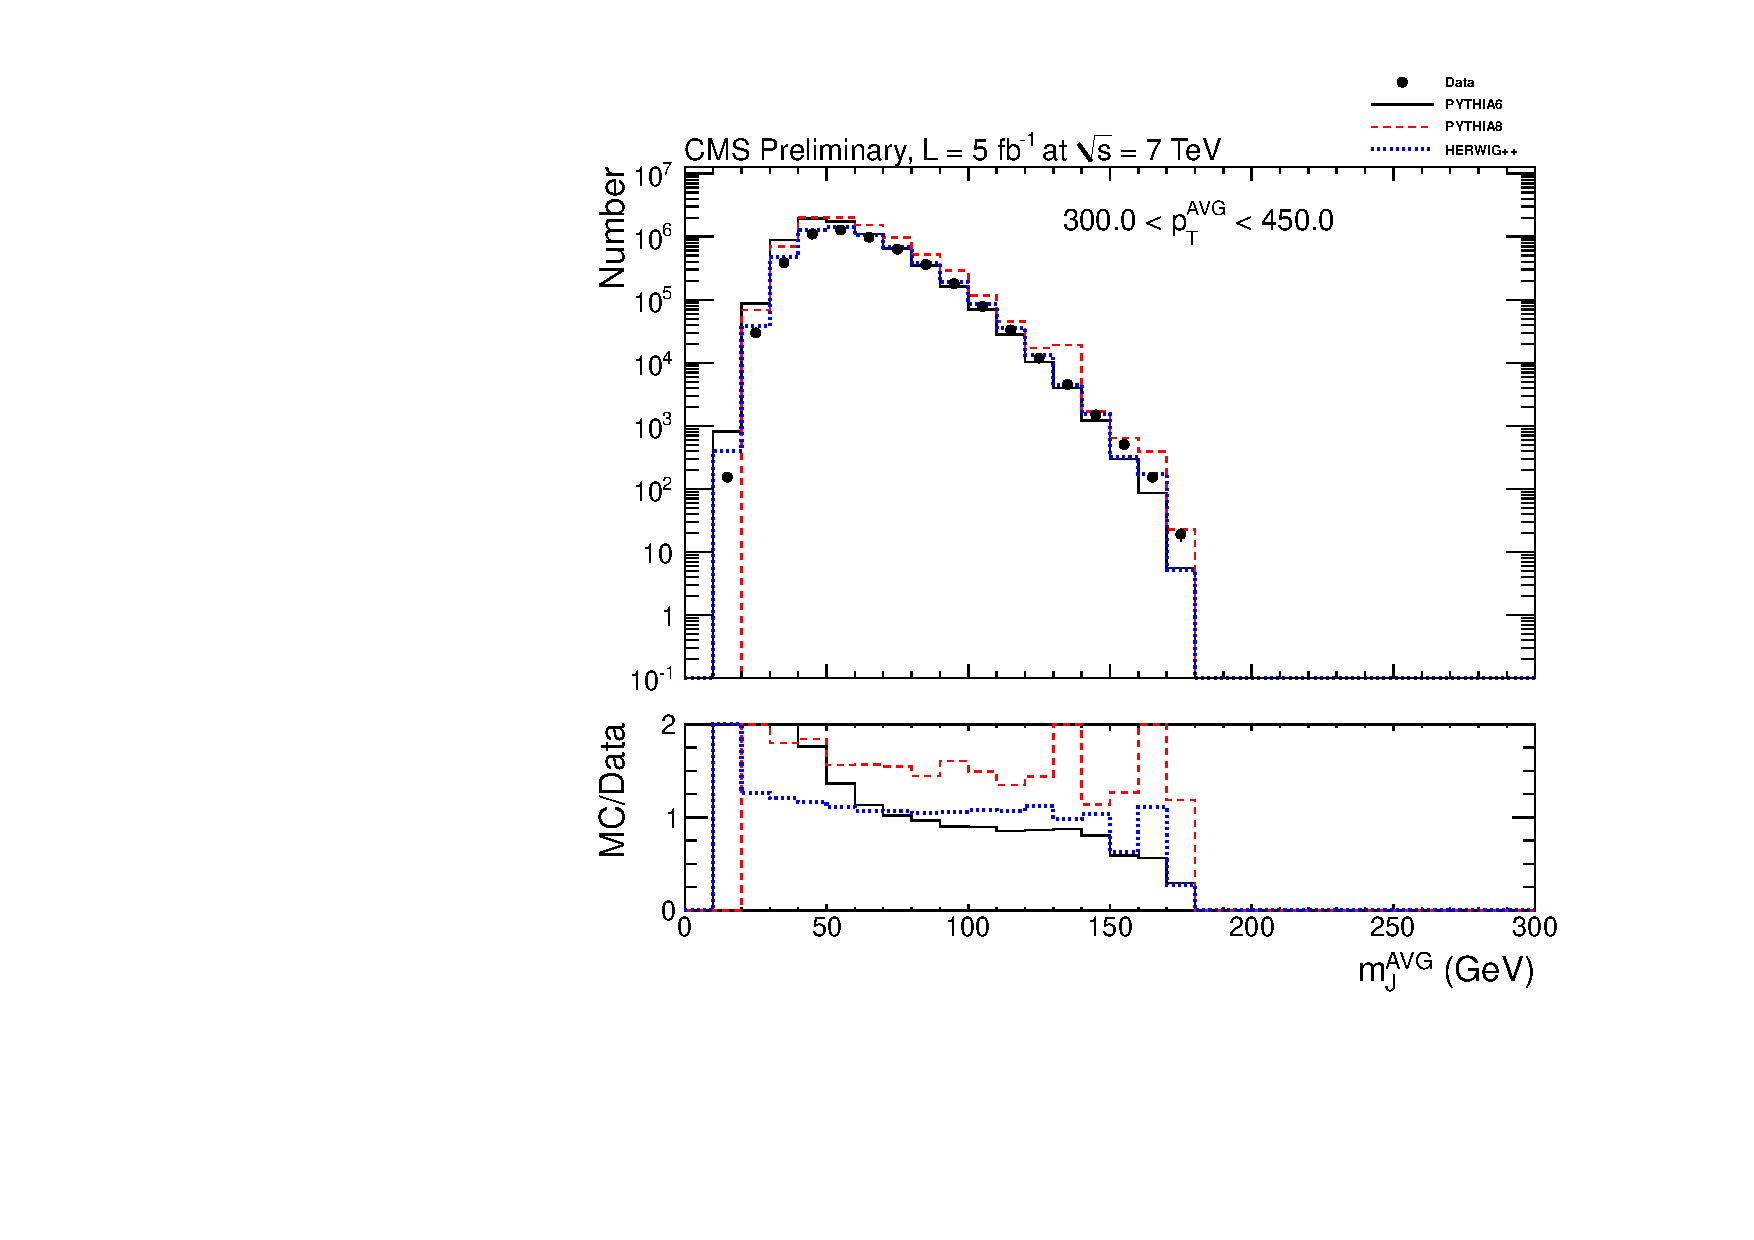
\includegraphics[width=0.95\textwidth]{figs/histAK7MjetVsPtAvg_rawDataMCComparisons_pt_5}
\caption{Detector-level distributions of the jet mass for AK7 jets,
for $300.0 < \pt^{AVG} < 450.0$ \GeVc. The data are shown in black points.
The simulated distribution from \PYTHIA is shown in solid black, 
the from \PYTHIAEIGHT in dashed red, and from \HERWIG in dotted blue. 
The bottom frame shows the ratio of the simulated distribution
to the distribution from data. 
\label{figs:histAK7MjetVsPtAvg_rawDataMCComparisons_pt_5}}
\end{figure}



\begin{figure}[htbp]
\centering
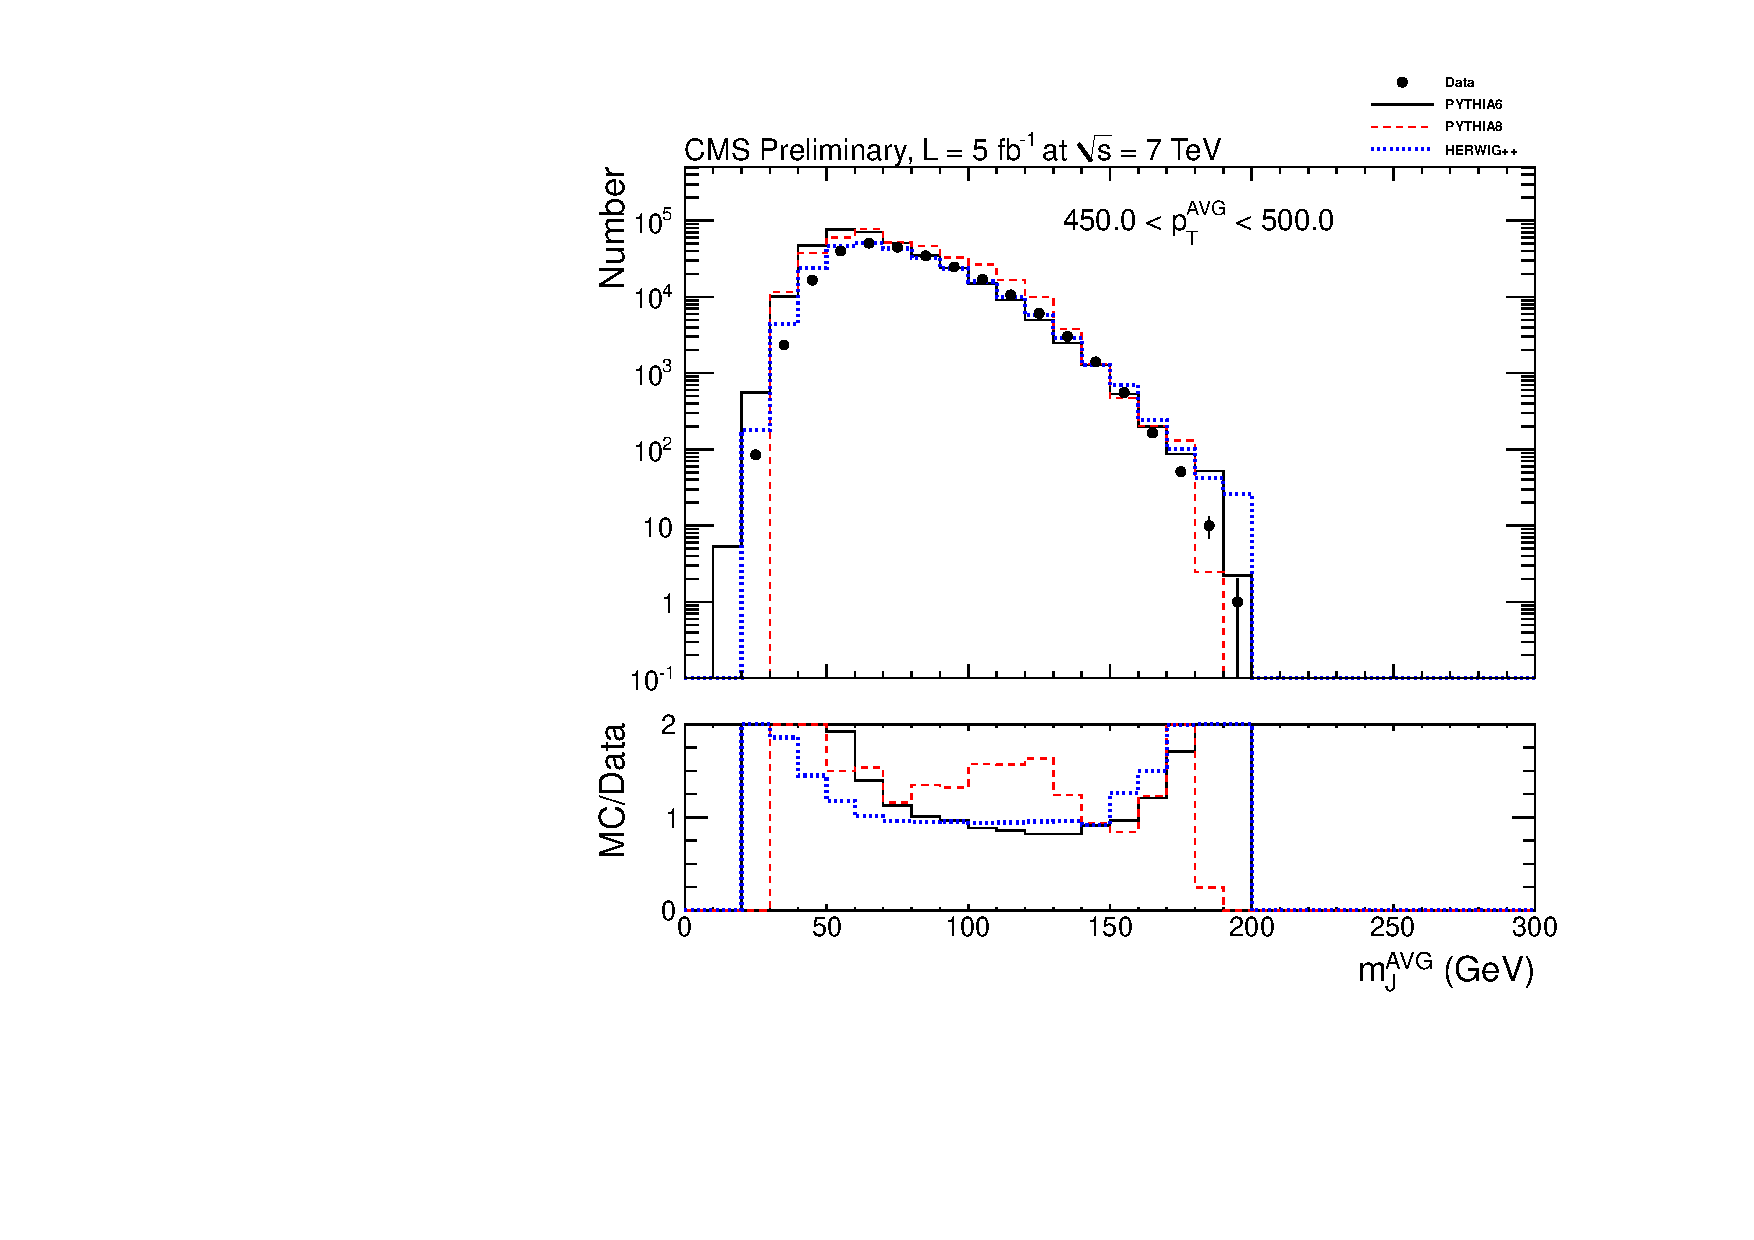
\includegraphics[width=0.95\textwidth]{figs/histAK7MjetVsPtAvg_rawDataMCComparisons_pt_6}
\caption{Detector-level distributions of the jet mass for AK7 jets,
for $450.0 < \pt^{AVG} < 500.0$ \GeVc. The data are shown in black points.
The simulated distribution from \PYTHIA is shown in solid black, 
the from \PYTHIAEIGHT in dashed red, and from \HERWIG in dotted blue. 
The bottom frame shows the ratio of the simulated distribution
to the distribution from data. 
\label{figs:histAK7MjetVsPtAvg_rawDataMCComparisons_pt_6}}
\end{figure}



\begin{figure}[htbp]
\centering
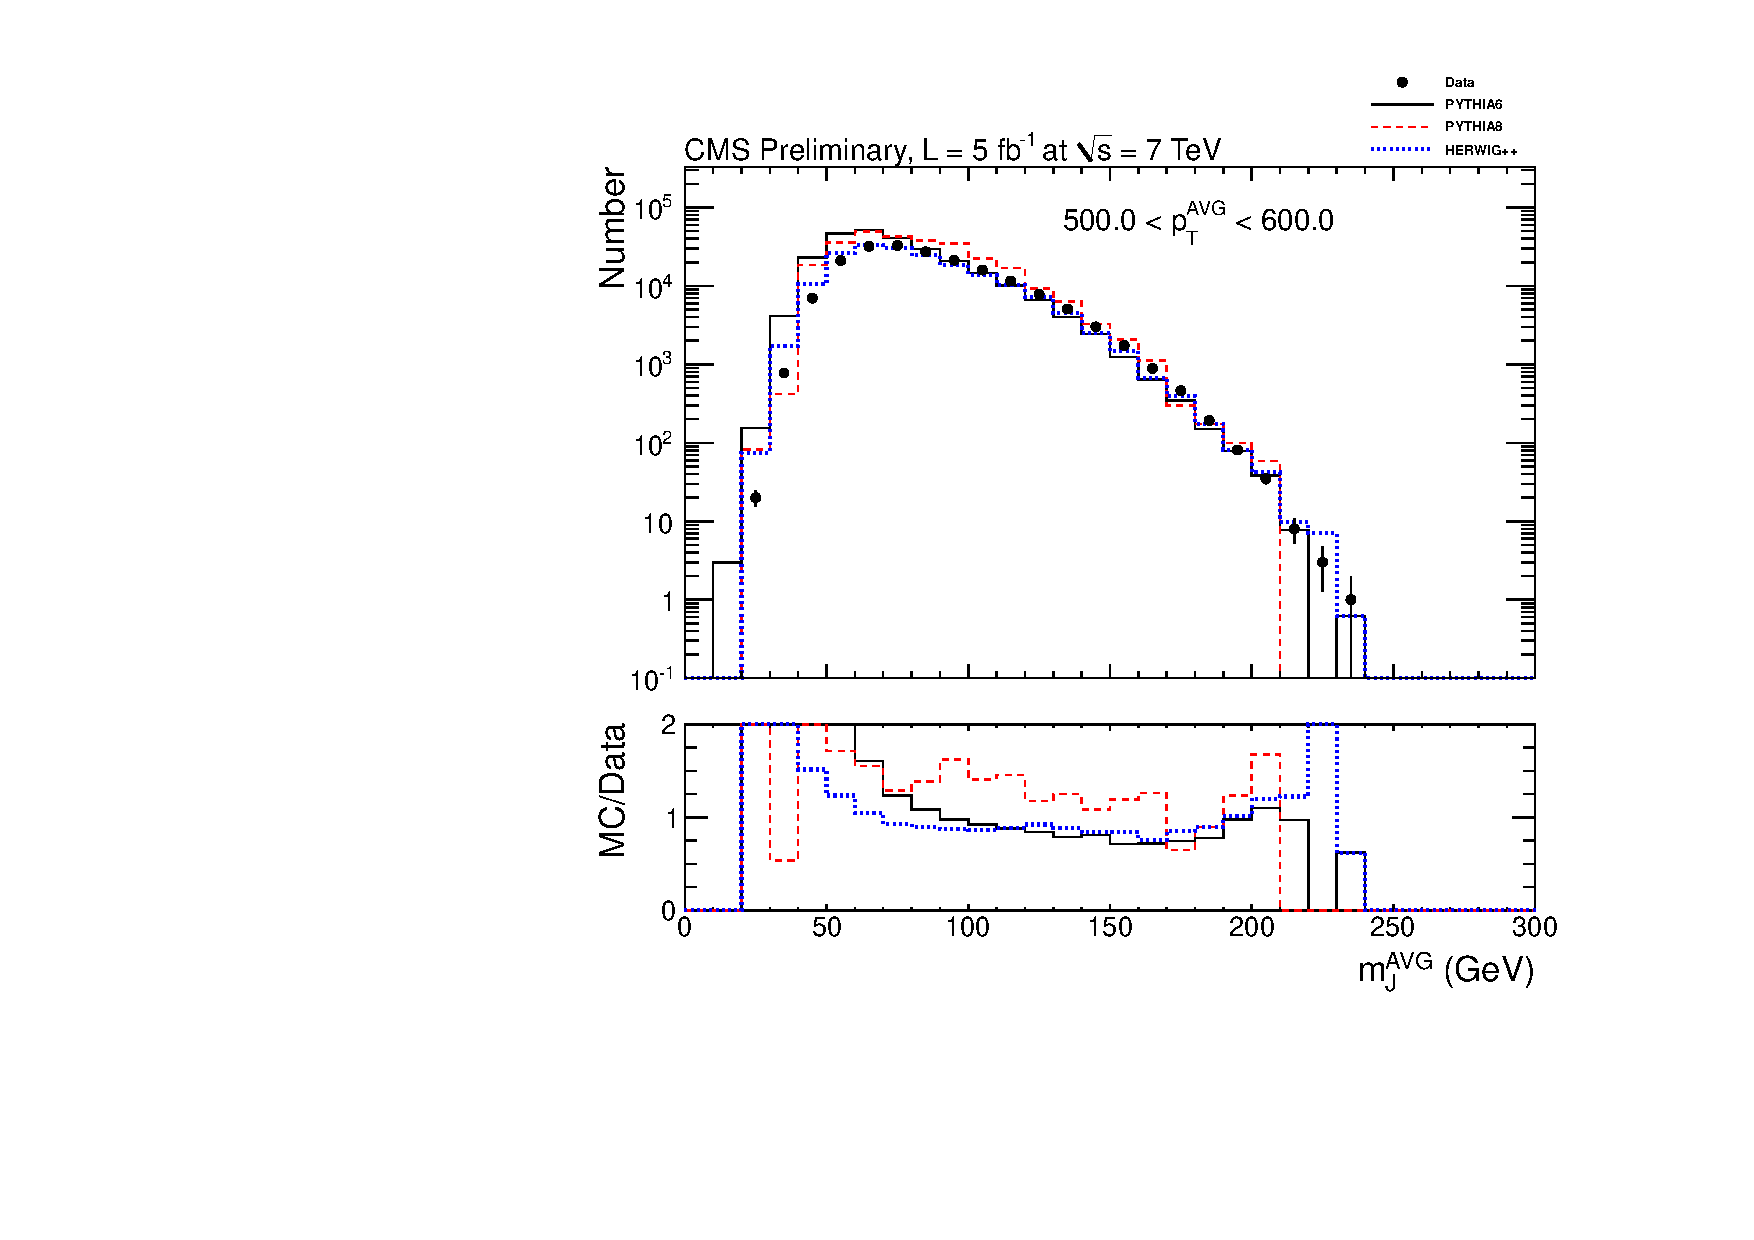
\includegraphics[width=0.95\textwidth]{figs/histAK7MjetVsPtAvg_rawDataMCComparisons_pt_7}
\caption{Detector-level distributions of the jet mass for AK7 jets,
for $500.0 < \pt^{AVG} < 600.0$ \GeVc. The data are shown in black points.
The simulated distribution from \PYTHIA is shown in solid black, 
the from \PYTHIAEIGHT in dashed red, and from \HERWIG in dotted blue. 
The bottom frame shows the ratio of the simulated distribution
to the distribution from data. 
\label{figs:histAK7MjetVsPtAvg_rawDataMCComparisons_pt_7}}
\end{figure}



\begin{figure}[htbp]
\centering
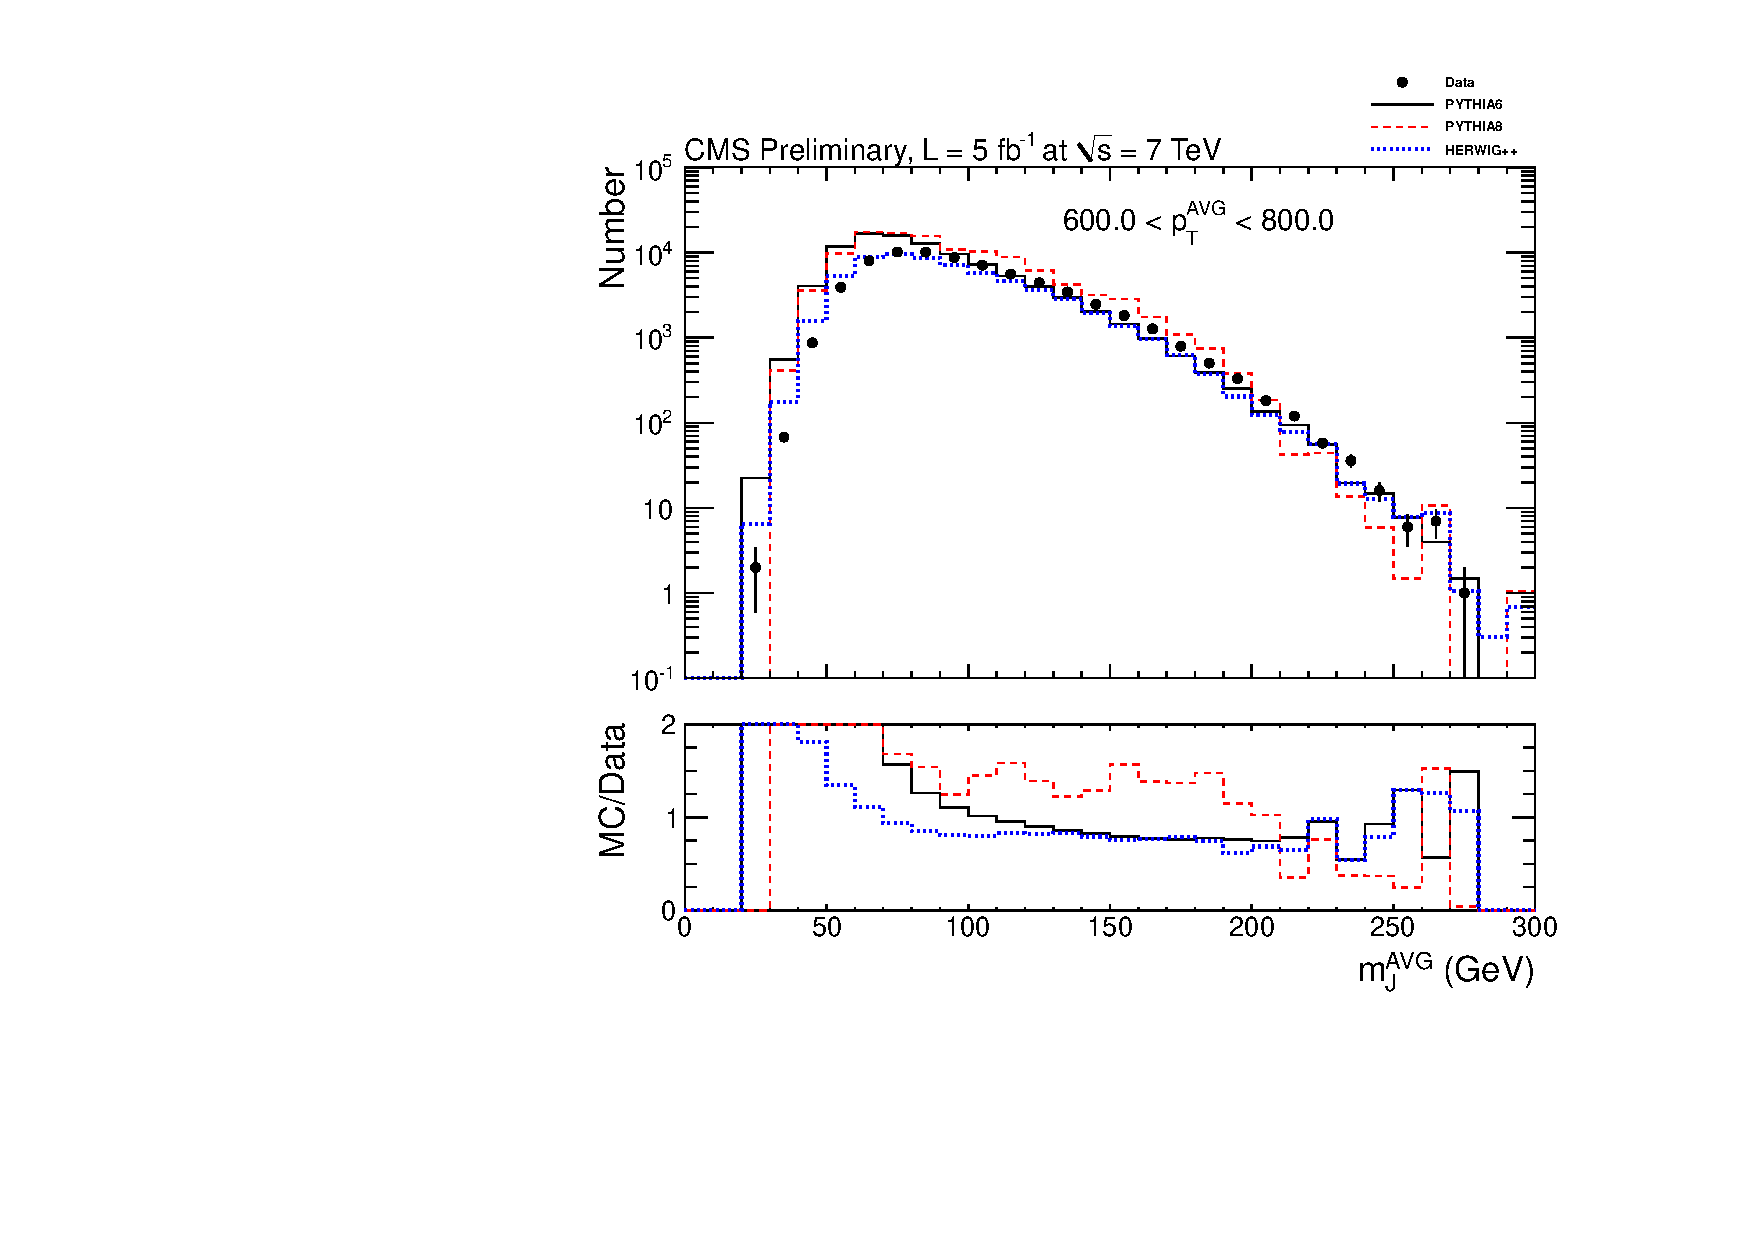
\includegraphics[width=0.95\textwidth]{figs/histAK7MjetVsPtAvg_rawDataMCComparisons_pt_8}
\caption{Detector-level distributions of the jet mass for AK7 jets,
for $600.0 < \pt^{AVG} < 800.0$ \GeVc. The data are shown in black points.
The simulated distribution from \PYTHIA is shown in solid black, 
the from \PYTHIAEIGHT in dashed red, and from \HERWIG in dotted blue. 
The bottom frame shows the ratio of the simulated distribution
to the distribution from data. 
\label{figs:histAK7MjetVsPtAvg_rawDataMCComparisons_pt_8}}
\end{figure}



\begin{figure}[htbp]
\centering
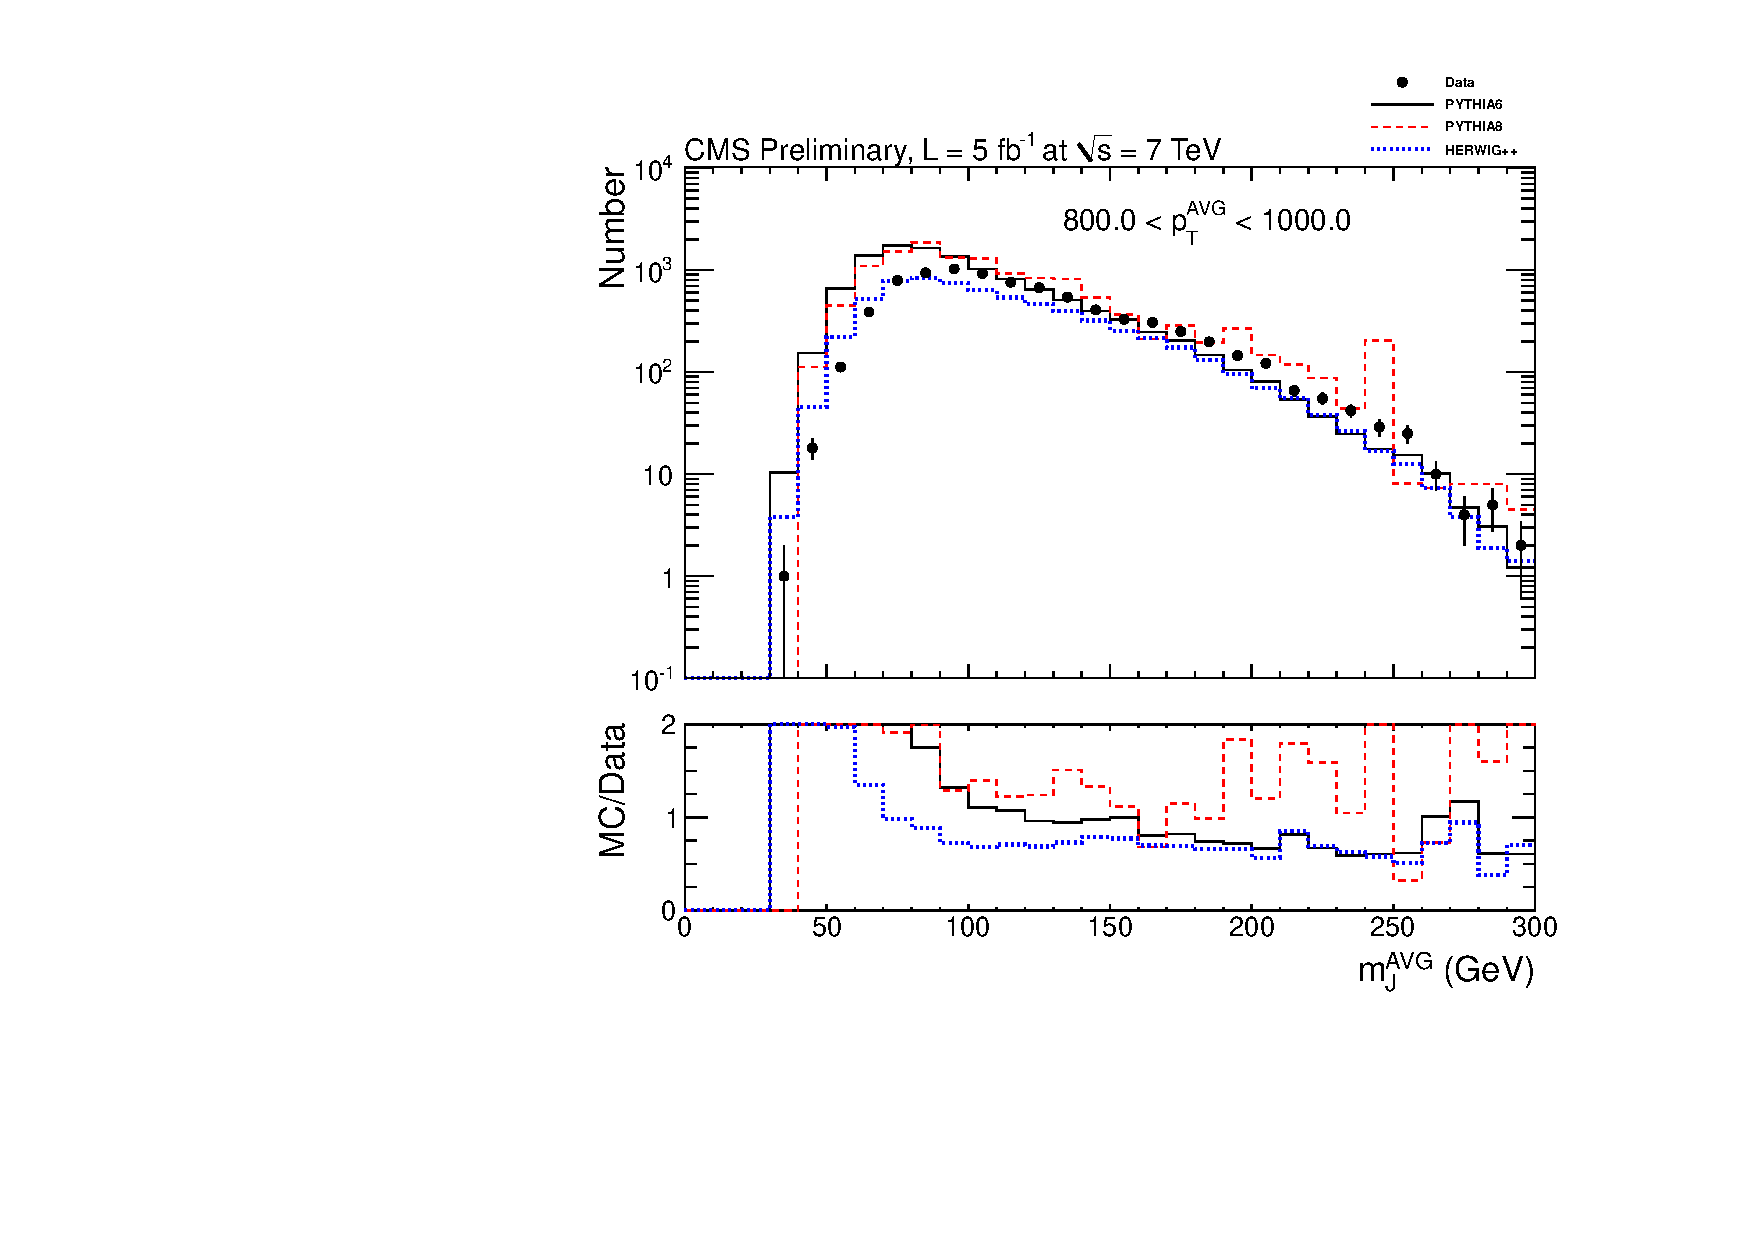
\includegraphics[width=0.95\textwidth]{figs/histAK7MjetVsPtAvg_rawDataMCComparisons_pt_9}
\caption{Detector-level distributions of the jet mass for AK7 jets,
for $800.0 < \pt^{AVG} < 1000.0$ \GeVc. The data are shown in black points.
The simulated distribution from \PYTHIA is shown in solid black, 
the from \PYTHIAEIGHT in dashed red, and from \HERWIG in dotted blue. 
The bottom frame shows the ratio of the simulated distribution
to the distribution from data. 
\label{figs:histAK7MjetVsPtAvg_rawDataMCComparisons_pt_9}}
\end{figure}



\begin{figure}[htbp]
\centering
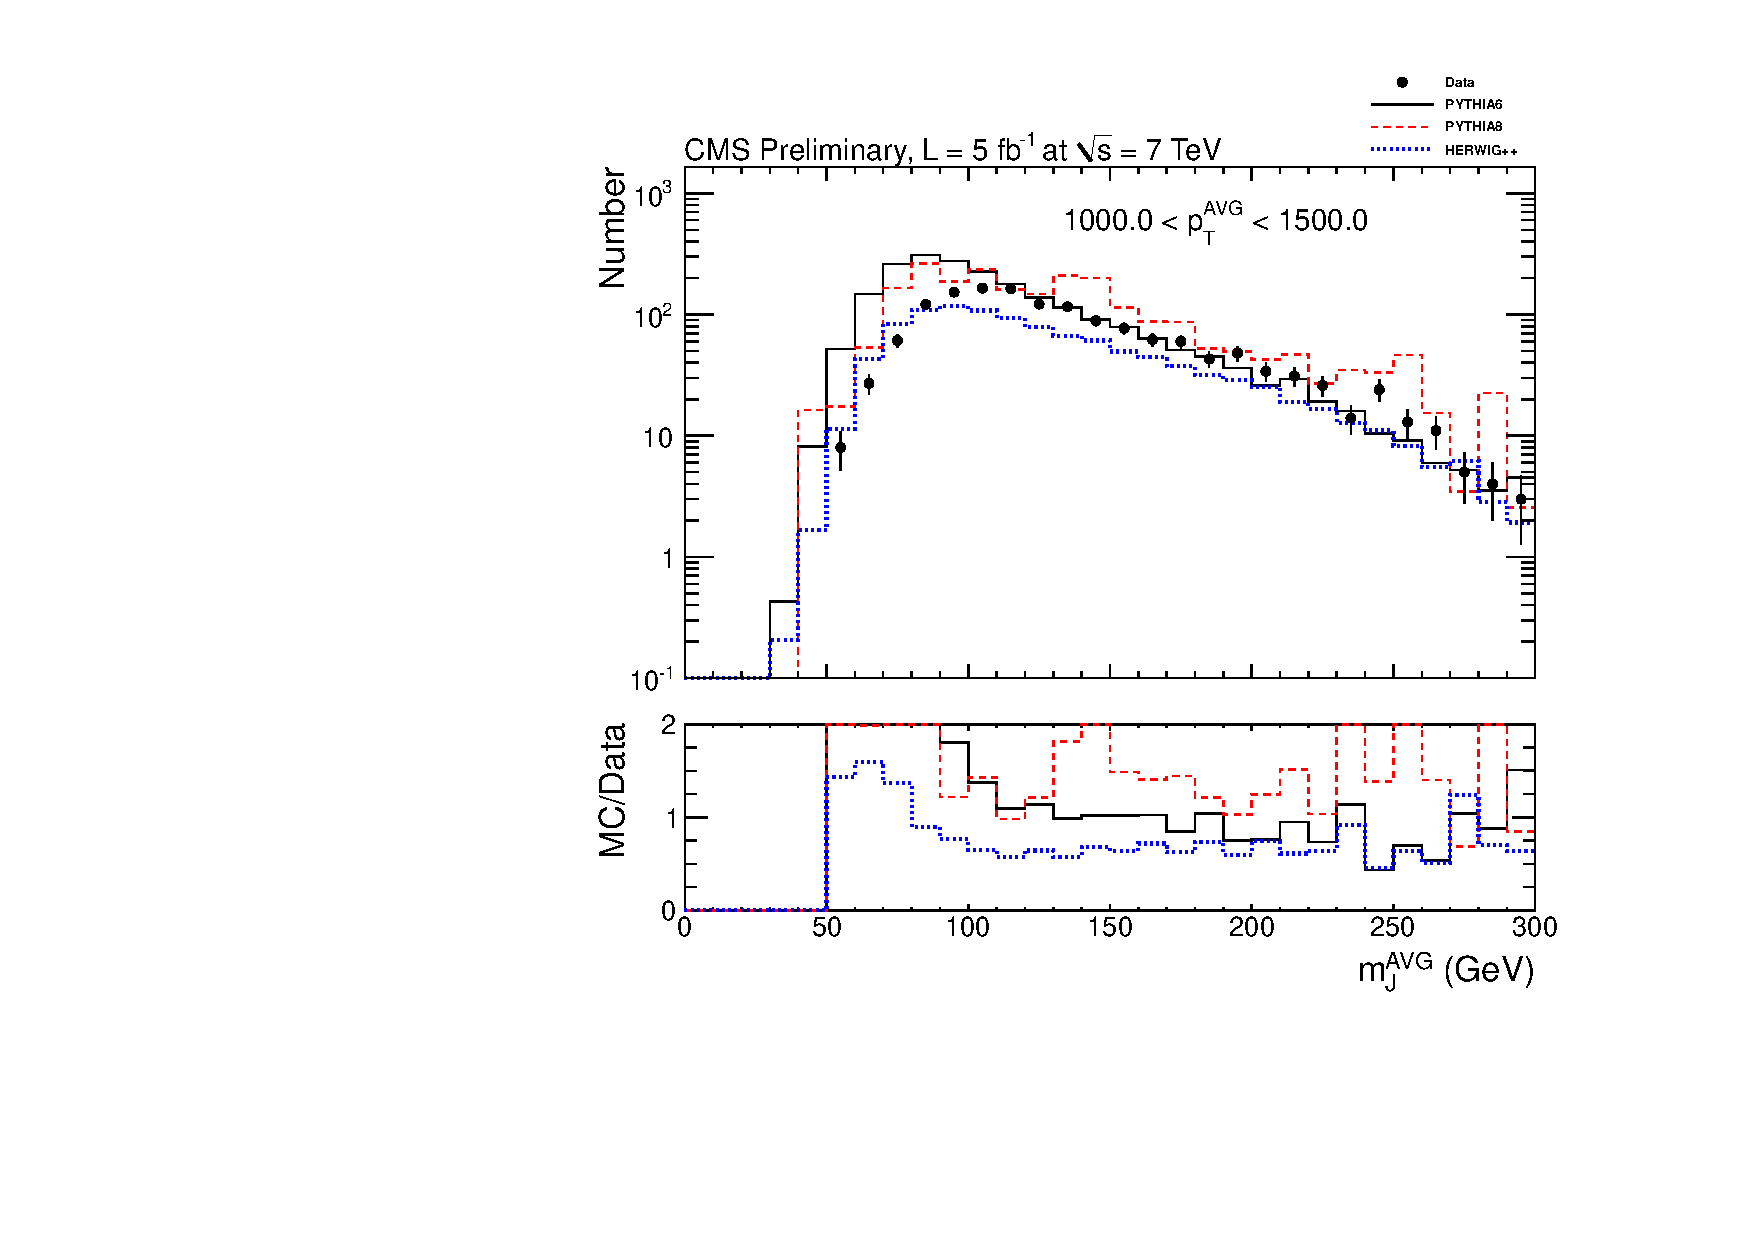
\includegraphics[width=0.95\textwidth]{figs/histAK7MjetVsPtAvg_rawDataMCComparisons_pt_10}
\caption{Detector-level distributions of the jet mass for AK7 jets,
for $1000.0 < \pt^{AVG} < 1500.0$ \GeVc. The data are shown in black points.
The simulated distribution from \PYTHIA is shown in solid black, 
the from \PYTHIAEIGHT in dashed red, and from \HERWIG in dotted blue. 
The bottom frame shows the ratio of the simulated distribution
to the distribution from data. 
\label{figs:histAK7MjetVsPtAvg_rawDataMCComparisons_pt_10}}
\end{figure}


\clearpage




\begin{figure}[htbp]
\centering
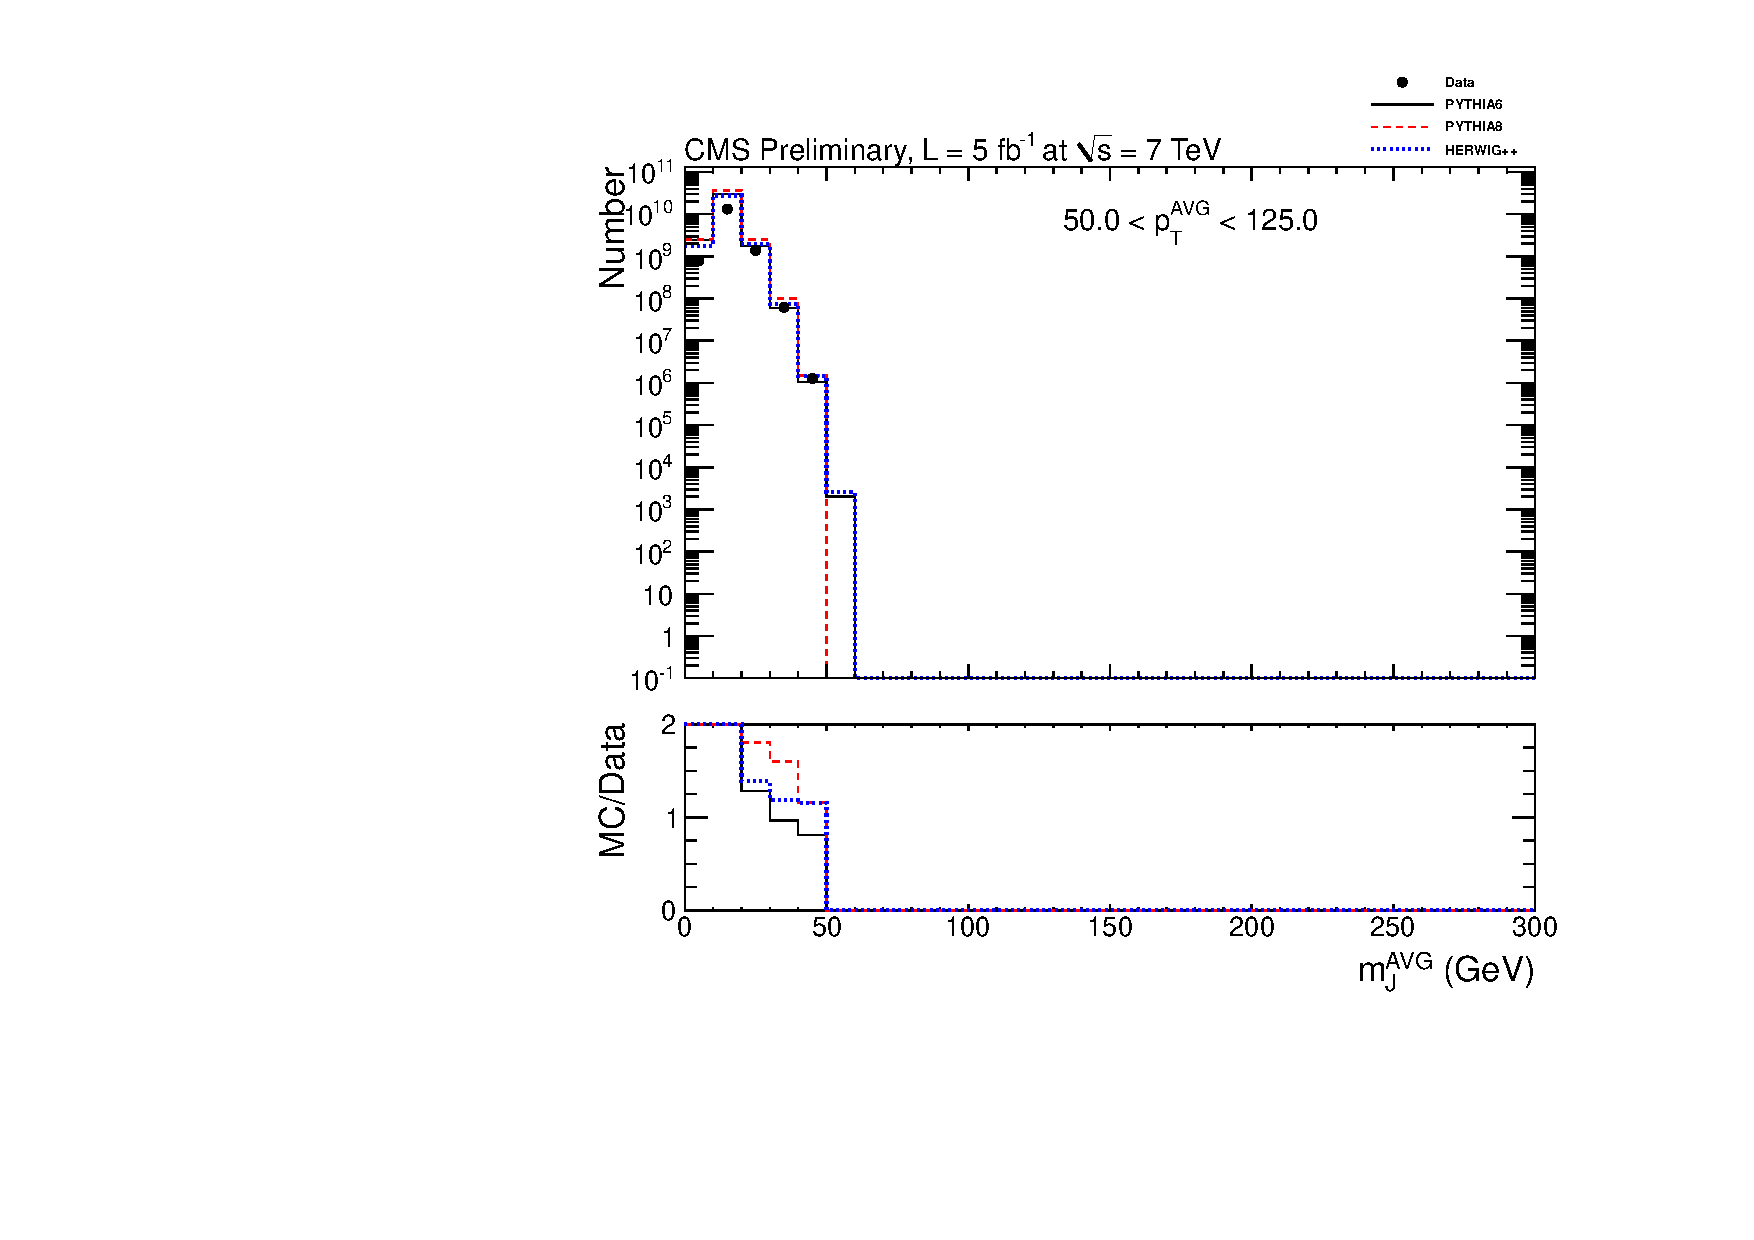
\includegraphics[width=0.95\textwidth]{figs/histAK7MjetVsPtAvg_rawDataMCComparisons_pt_1_Filtered}
\caption{Detector-level distributions of the jet mass for AK7 Filtered jets,
for $50.0 < \pt^{AVG} < 125.0$ \GeVc. The data are shown in black points.
The simulated distribution from \PYTHIA is shown in solid black, 
the from \PYTHIAEIGHT in dashed red, and from \HERWIG in dotted blue. 
The bottom frame shows the ratio of the simulated distribution
to the distribution from data. 
\label{figs:histAK7MjetVsPtAvg_rawDataMCComparisons_pt_1_Filtered}}
\end{figure}



\begin{figure}[htbp]
\centering
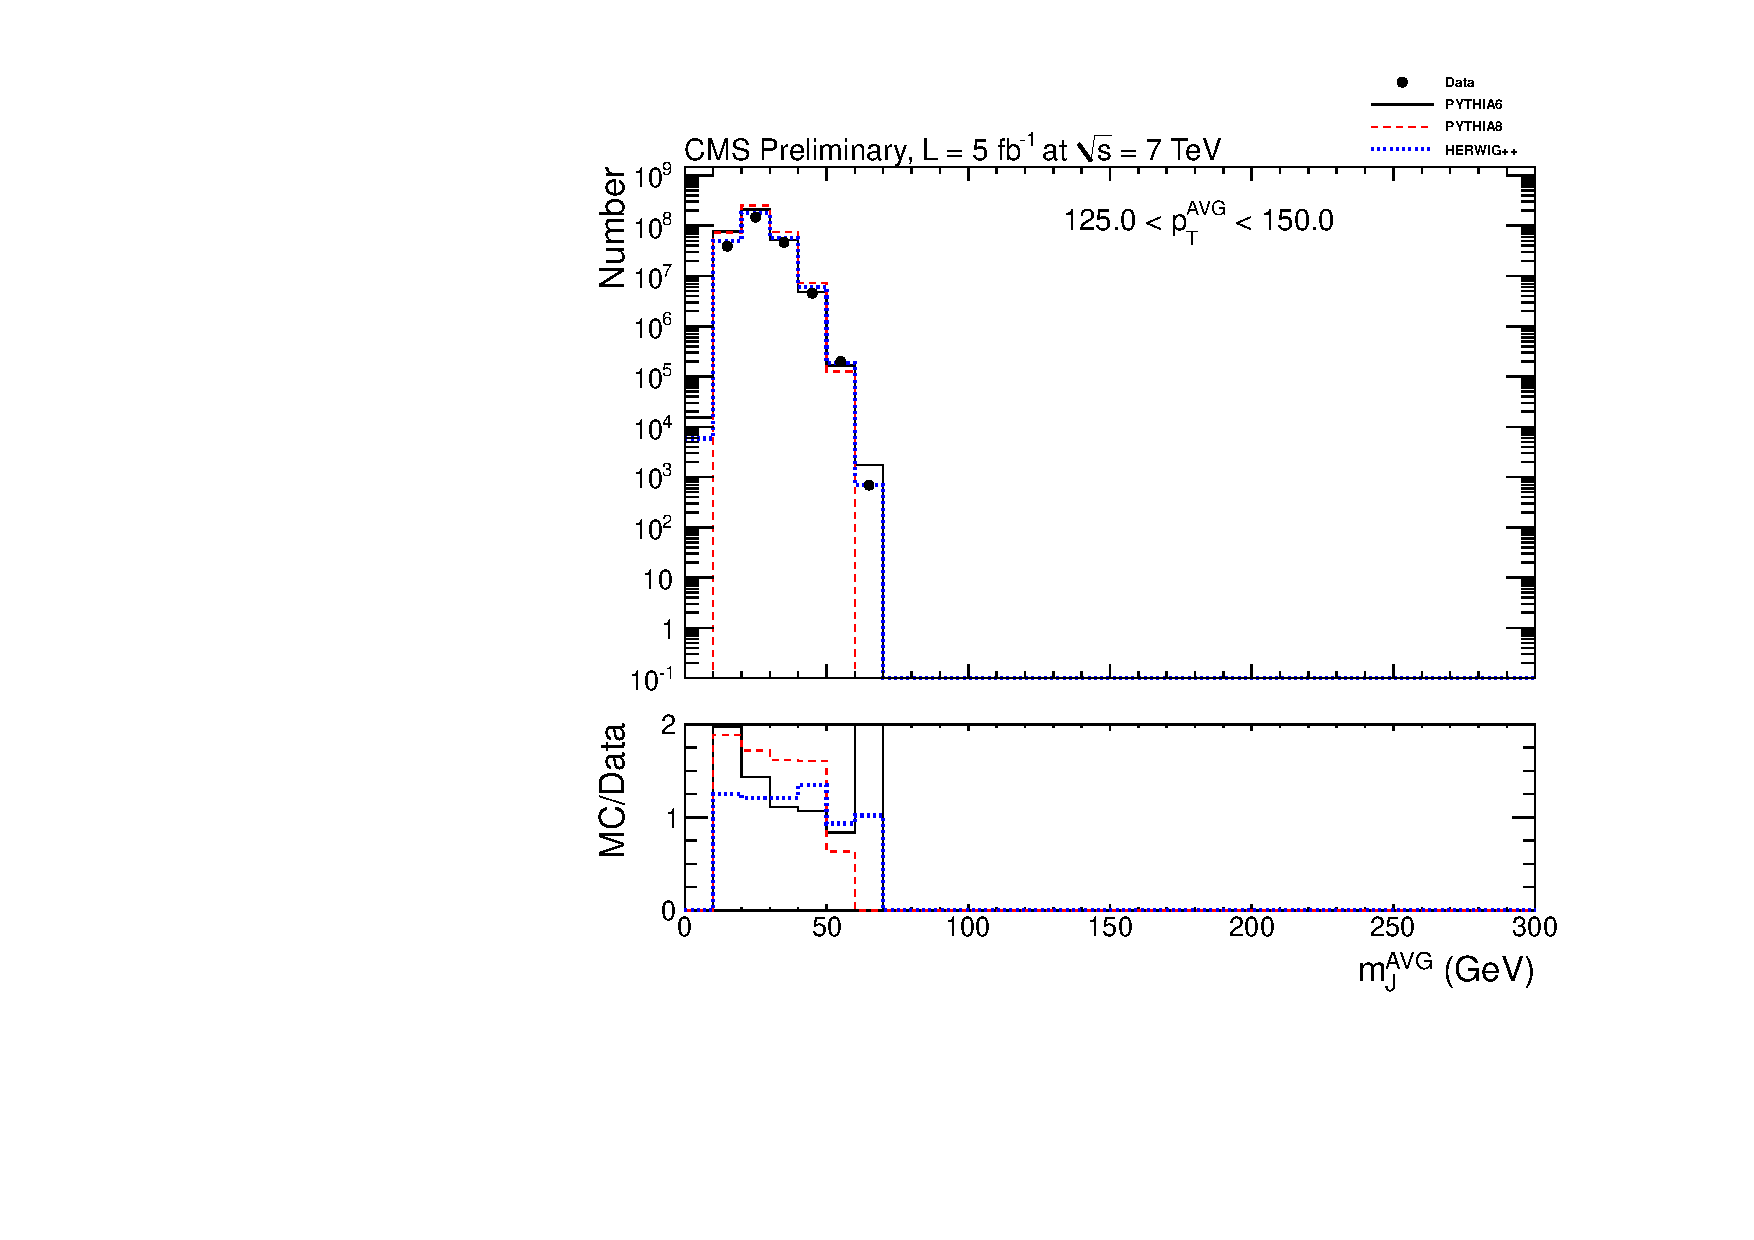
\includegraphics[width=0.95\textwidth]{figs/histAK7MjetVsPtAvg_rawDataMCComparisons_pt_2_Filtered}
\caption{Detector-level distributions of the jet mass for AK7 Filtered jets,
for $125.0 < \pt^{AVG} < 150.0$ \GeVc. The data are shown in black points.
The simulated distribution from \PYTHIA is shown in solid black, 
the from \PYTHIAEIGHT in dashed red, and from \HERWIG in dotted blue. 
The bottom frame shows the ratio of the simulated distribution
to the distribution from data. 
\label{figs:histAK7MjetVsPtAvg_rawDataMCComparisons_pt_2_Filtered}}
\end{figure}



\begin{figure}[htbp]
\centering
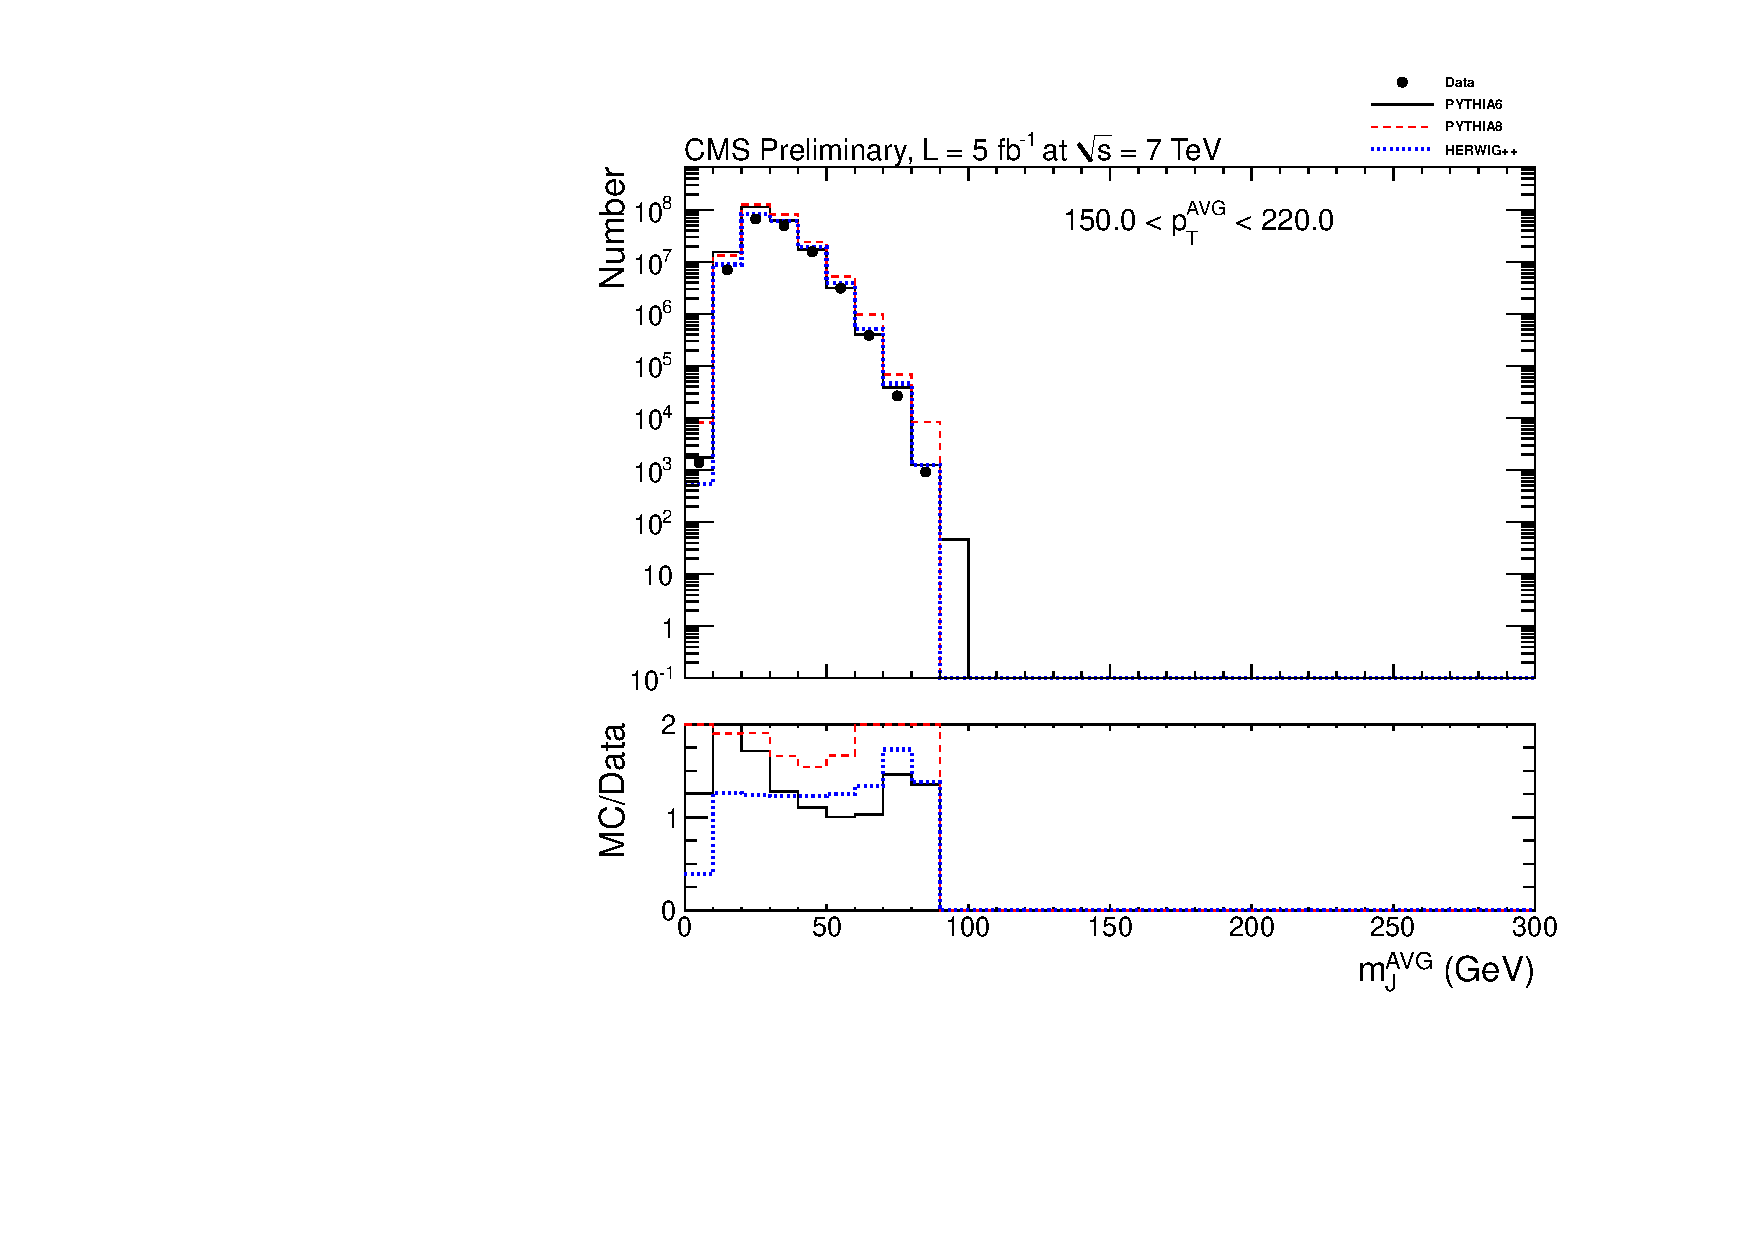
\includegraphics[width=0.95\textwidth]{figs/histAK7MjetVsPtAvg_rawDataMCComparisons_pt_3_Filtered}
\caption{Detector-level distributions of the jet mass for AK7 Filtered jets,
for $150.0 < \pt^{AVG} < 220.0$ \GeVc. The data are shown in black points.
The simulated distribution from \PYTHIA is shown in solid black, 
the from \PYTHIAEIGHT in dashed red, and from \HERWIG in dotted blue. 
The bottom frame shows the ratio of the simulated distribution
to the distribution from data. 
\label{figs:histAK7MjetVsPtAvg_rawDataMCComparisons_pt_3_Filtered}}
\end{figure}



\begin{figure}[htbp]
\centering
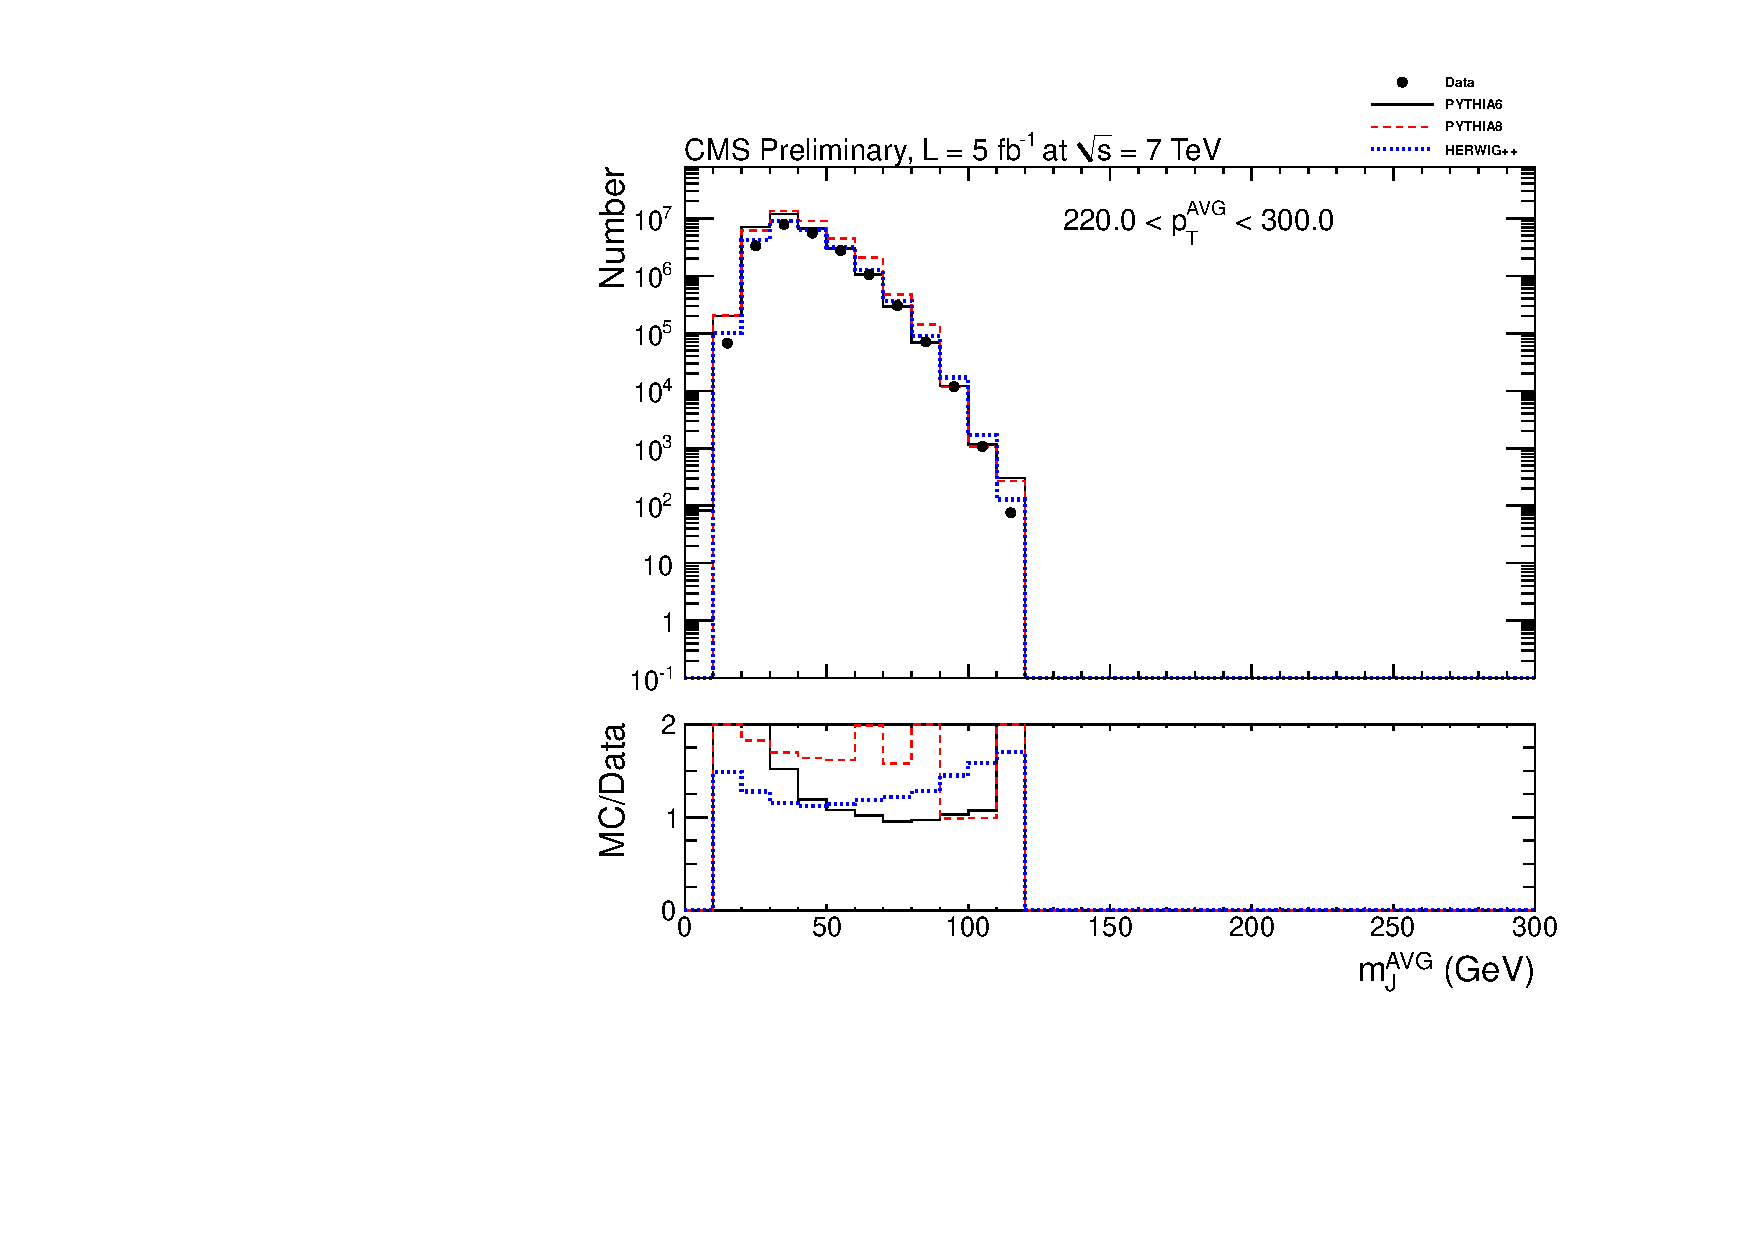
\includegraphics[width=0.95\textwidth]{figs/histAK7MjetVsPtAvg_rawDataMCComparisons_pt_4_Filtered}
\caption{Detector-level distributions of the jet mass for AK7 Filtered jets,
for $220.0 < \pt^{AVG} < 300.0$ \GeVc. The data are shown in black points.
The simulated distribution from \PYTHIA is shown in solid black, 
the from \PYTHIAEIGHT in dashed red, and from \HERWIG in dotted blue. 
The bottom frame shows the ratio of the simulated distribution
to the distribution from data. 
\label{figs:histAK7MjetVsPtAvg_rawDataMCComparisons_pt_4_Filtered}}
\end{figure}



\begin{figure}[htbp]
\centering
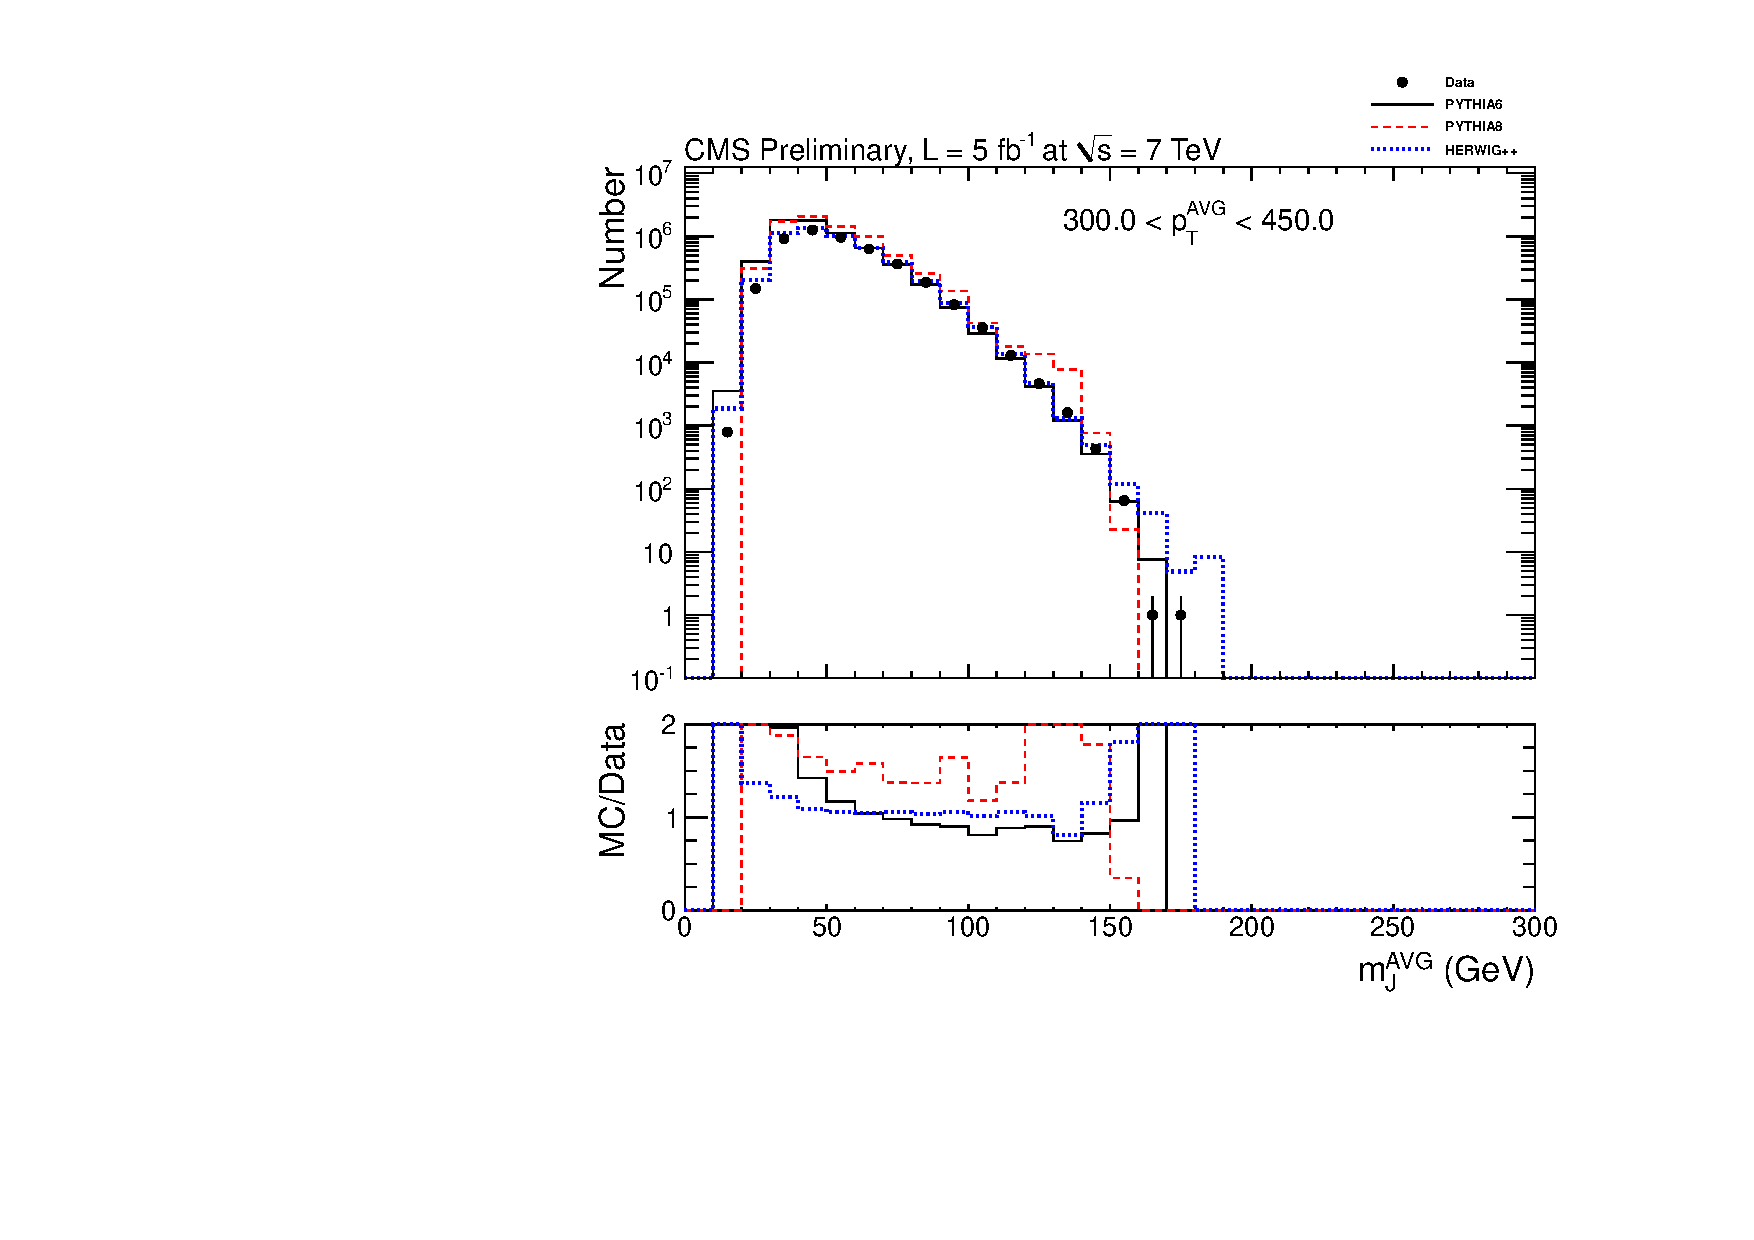
\includegraphics[width=0.95\textwidth]{figs/histAK7MjetVsPtAvg_rawDataMCComparisons_pt_5_Filtered}
\caption{Detector-level distributions of the jet mass for AK7 Filtered jets,
for $300.0 < \pt^{AVG} < 450.0$ \GeVc. The data are shown in black points.
The simulated distribution from \PYTHIA is shown in solid black, 
the from \PYTHIAEIGHT in dashed red, and from \HERWIG in dotted blue. 
The bottom frame shows the ratio of the simulated distribution
to the distribution from data. 
\label{figs:histAK7MjetVsPtAvg_rawDataMCComparisons_pt_5_Filtered}}
\end{figure}



\begin{figure}[htbp]
\centering
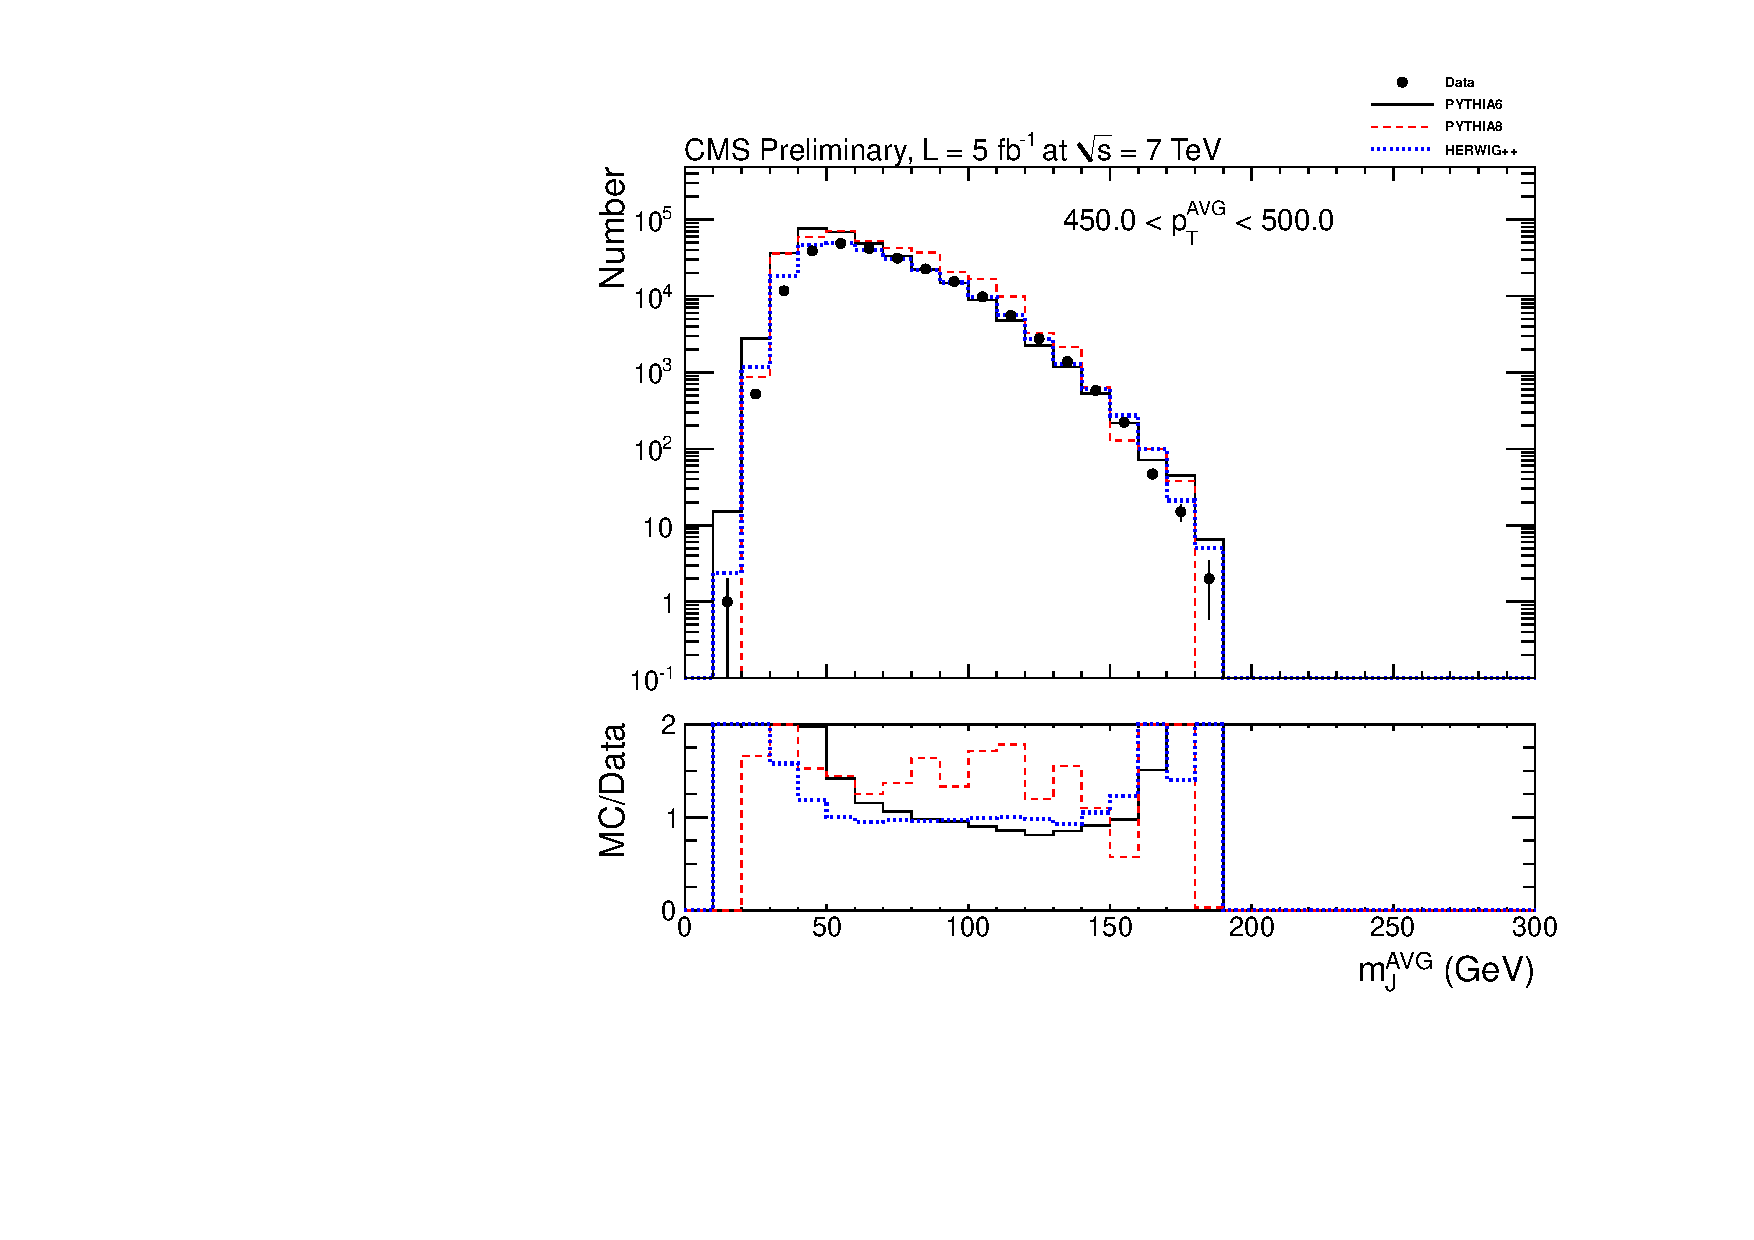
\includegraphics[width=0.95\textwidth]{figs/histAK7MjetVsPtAvg_rawDataMCComparisons_pt_6_Filtered}
\caption{Detector-level distributions of the jet mass for AK7 Filtered jets,
for $450.0 < \pt^{AVG} < 500.0$ \GeVc. The data are shown in black points.
The simulated distribution from \PYTHIA is shown in solid black, 
the from \PYTHIAEIGHT in dashed red, and from \HERWIG in dotted blue. 
The bottom frame shows the ratio of the simulated distribution
to the distribution from data. 
\label{figs:histAK7MjetVsPtAvg_rawDataMCComparisons_pt_6_Filtered}}
\end{figure}



\begin{figure}[htbp]
\centering
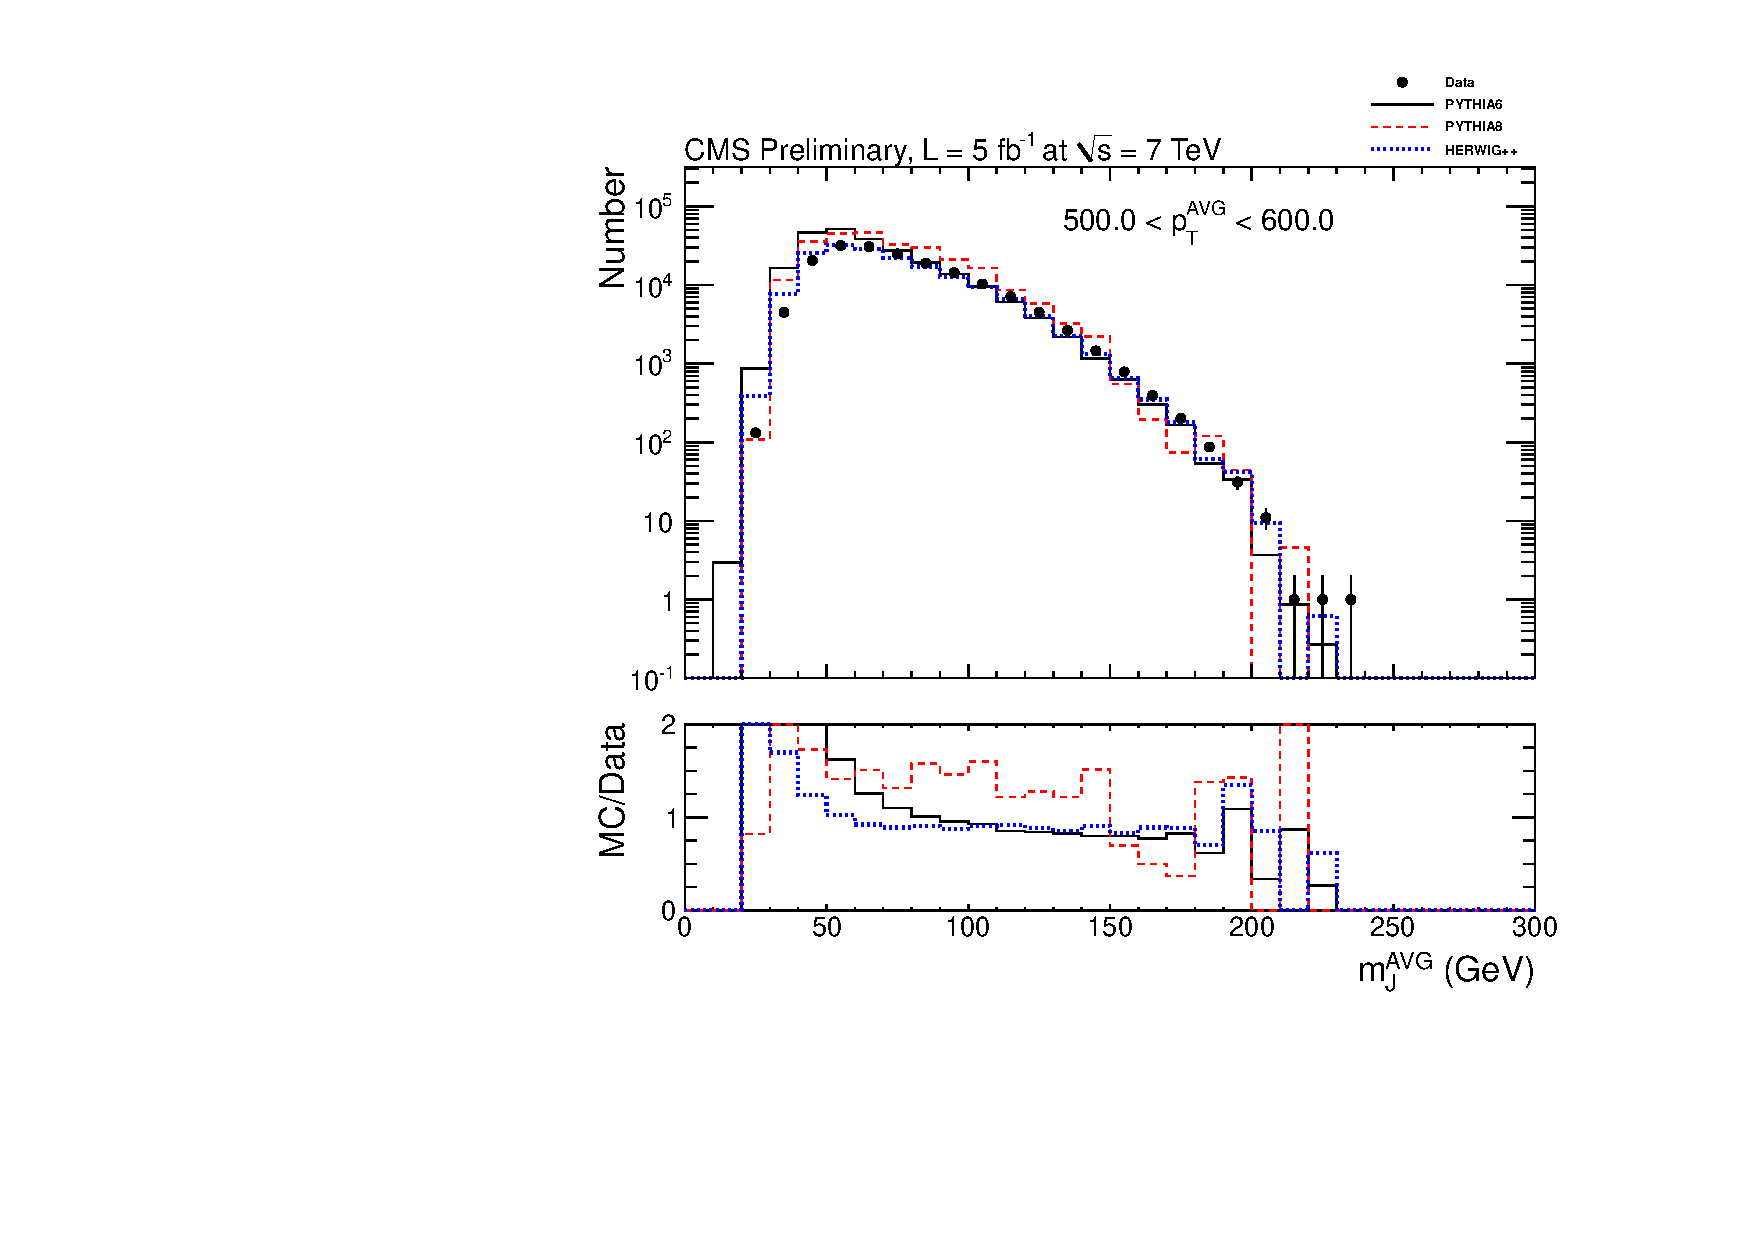
\includegraphics[width=0.95\textwidth]{figs/histAK7MjetVsPtAvg_rawDataMCComparisons_pt_7_Filtered}
\caption{Detector-level distributions of the jet mass for AK7 Filtered jets,
for $500.0 < \pt^{AVG} < 600.0$ \GeVc. The data are shown in black points.
The simulated distribution from \PYTHIA is shown in solid black, 
the from \PYTHIAEIGHT in dashed red, and from \HERWIG in dotted blue. 
The bottom frame shows the ratio of the simulated distribution
to the distribution from data. 
\label{figs:histAK7MjetVsPtAvg_rawDataMCComparisons_pt_7_Filtered}}
\end{figure}



\begin{figure}[htbp]
\centering
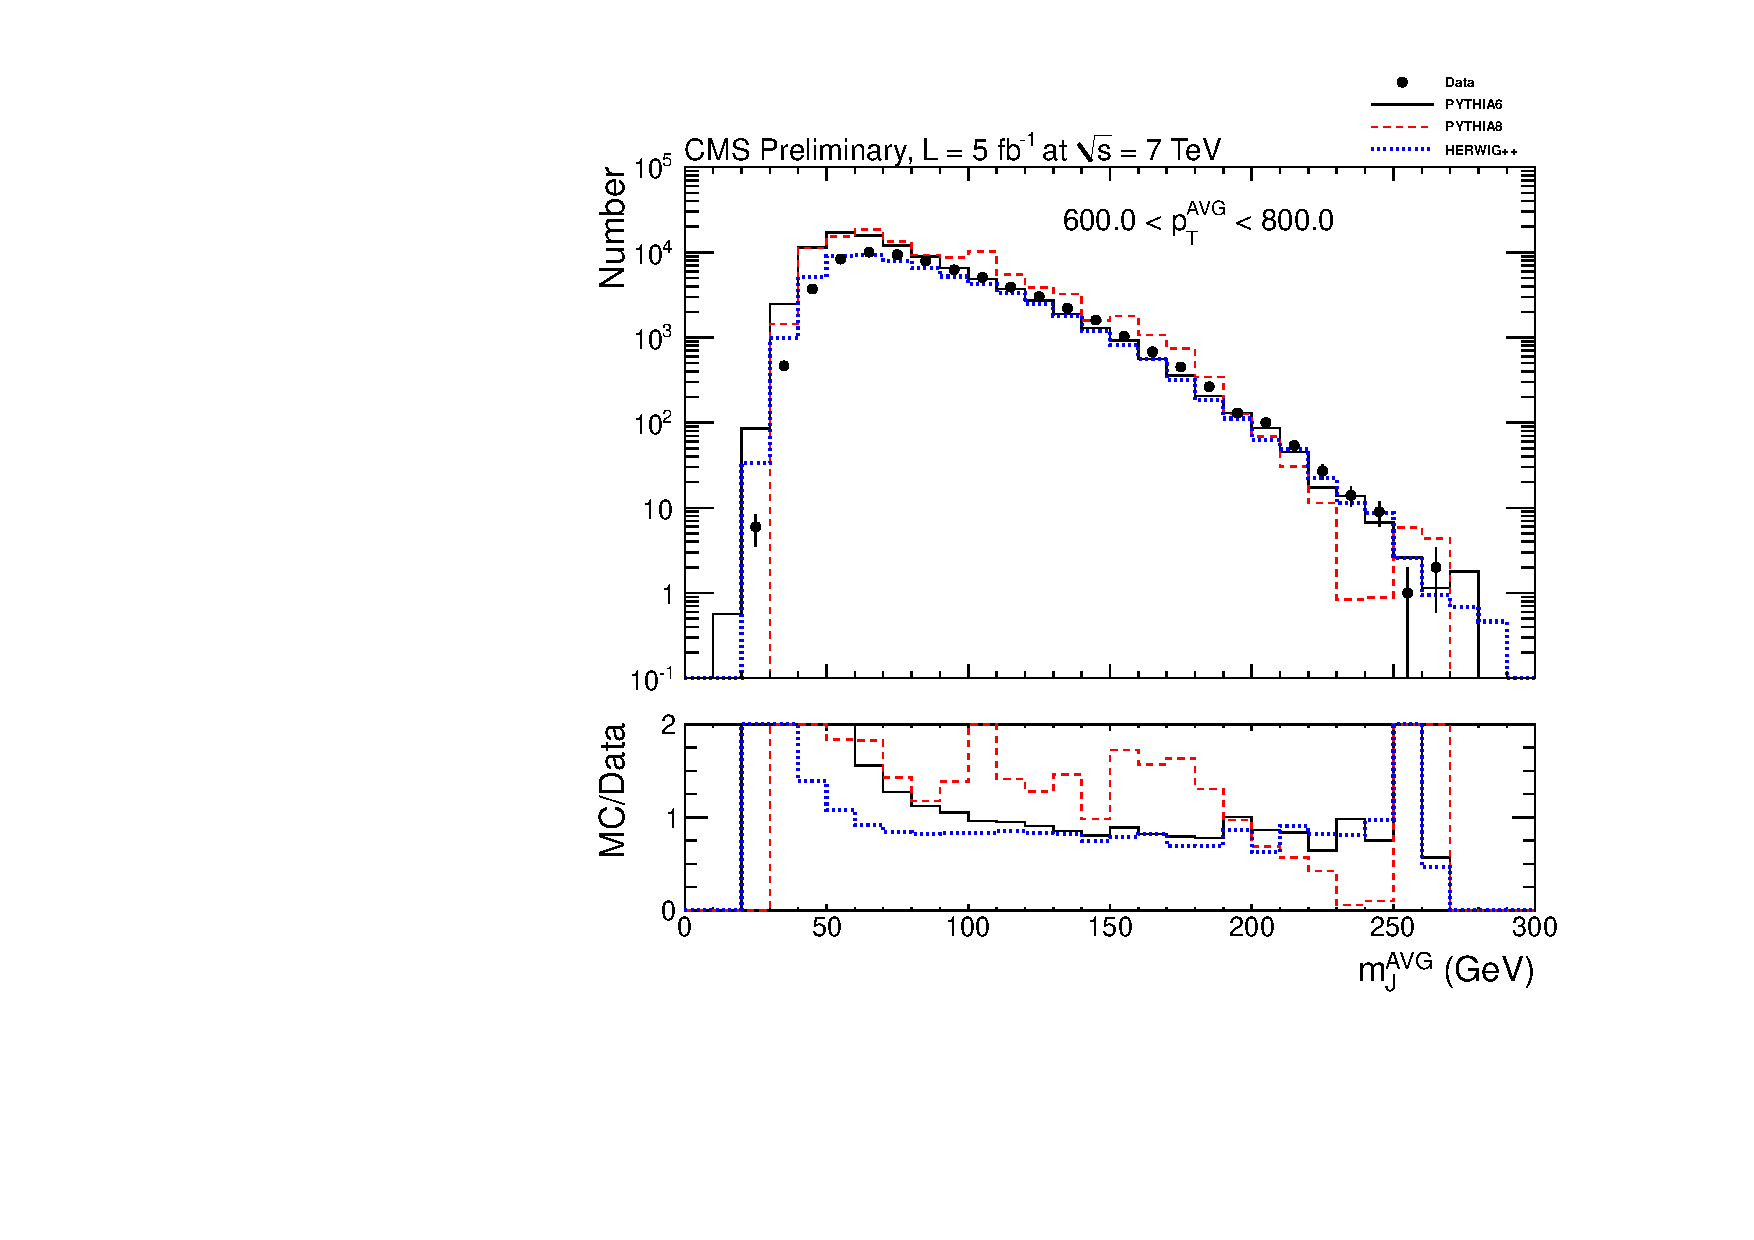
\includegraphics[width=0.95\textwidth]{figs/histAK7MjetVsPtAvg_rawDataMCComparisons_pt_8_Filtered}
\caption{Detector-level distributions of the jet mass for AK7 Filtered jets,
for $600.0 < \pt^{AVG} < 800.0$ \GeVc. The data are shown in black points.
The simulated distribution from \PYTHIA is shown in solid black, 
the from \PYTHIAEIGHT in dashed red, and from \HERWIG in dotted blue. 
The bottom frame shows the ratio of the simulated distribution
to the distribution from data. 
\label{figs:histAK7MjetVsPtAvg_rawDataMCComparisons_pt_8_Filtered}}
\end{figure}



\begin{figure}[htbp]
\centering
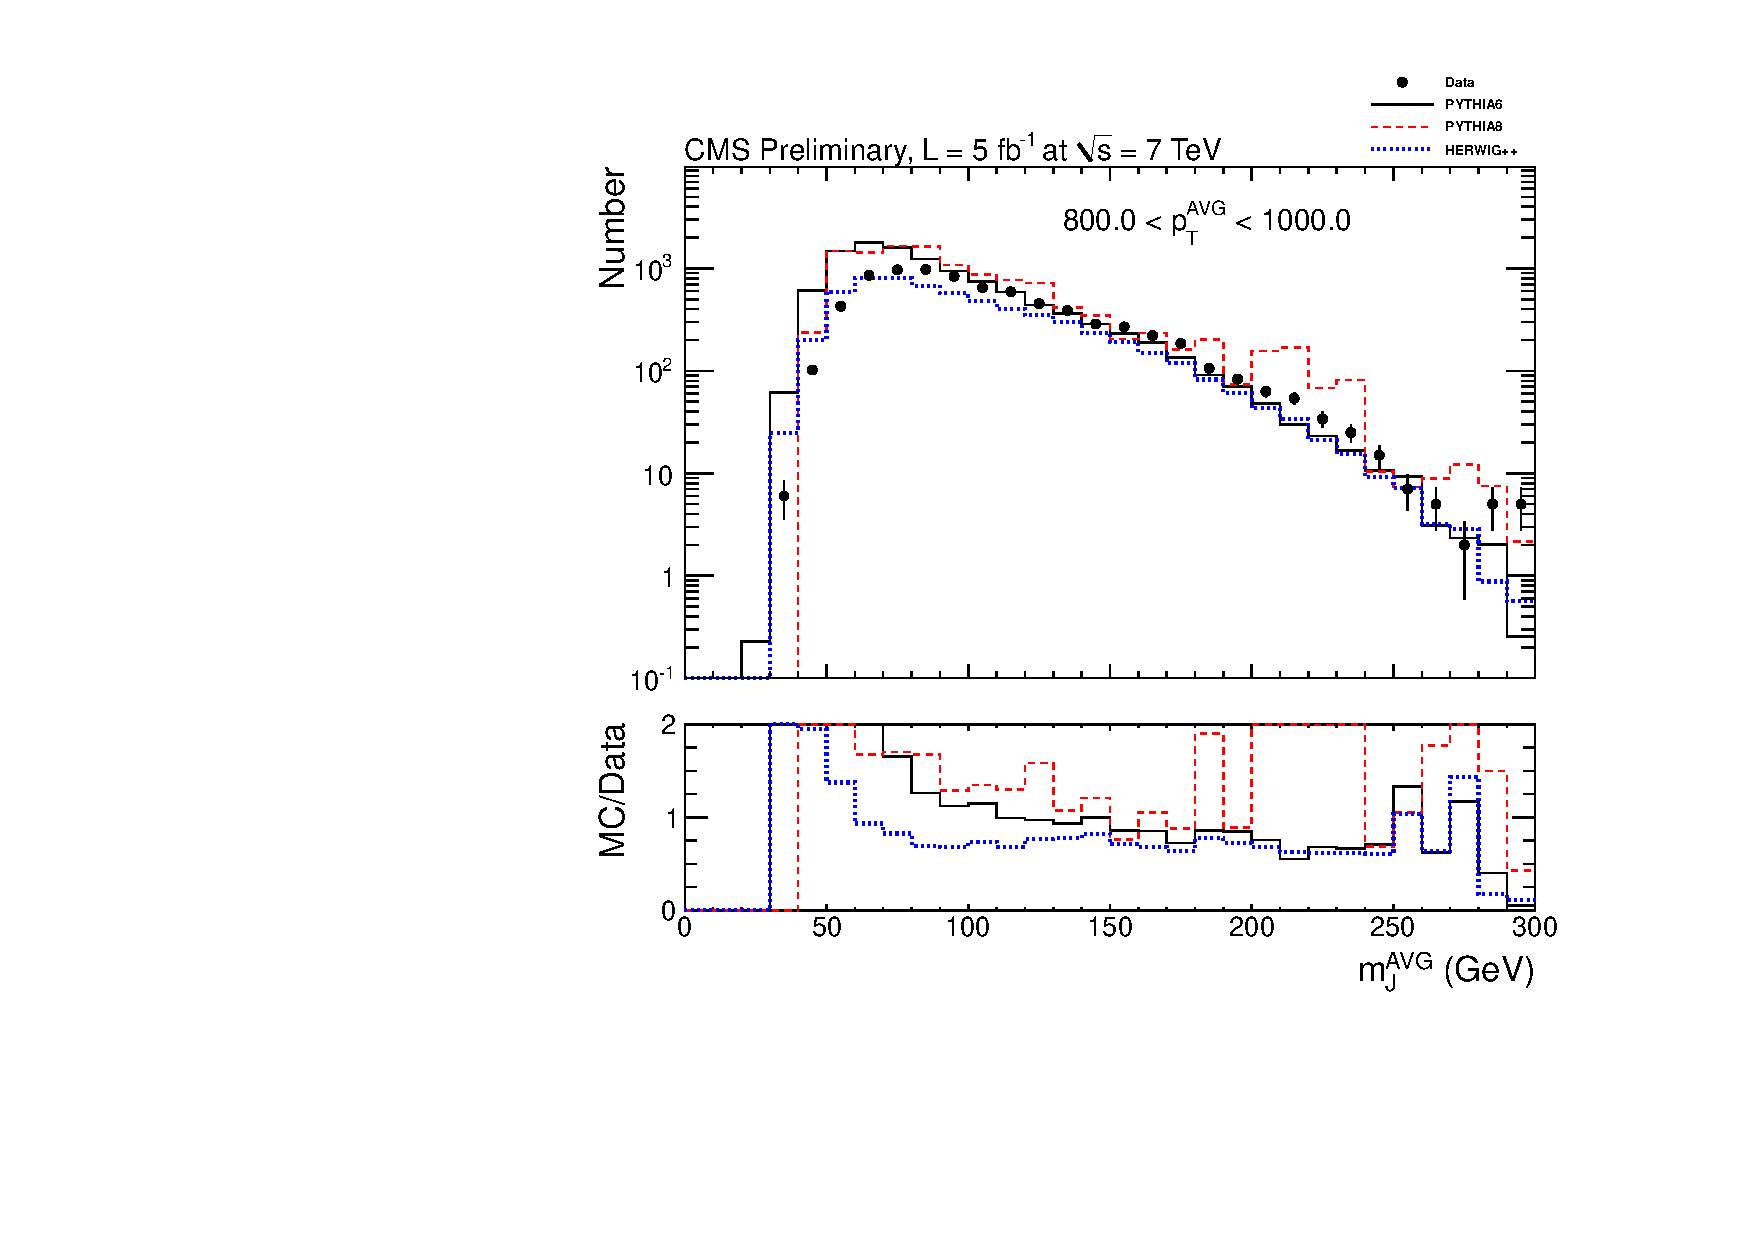
\includegraphics[width=0.95\textwidth]{figs/histAK7MjetVsPtAvg_rawDataMCComparisons_pt_9_Filtered}
\caption{Detector-level distributions of the jet mass for AK7 Filtered jets,
for $800.0 < \pt^{AVG} < 1000.0$ \GeVc. The data are shown in black points.
The simulated distribution from \PYTHIA is shown in solid black, 
the from \PYTHIAEIGHT in dashed red, and from \HERWIG in dotted blue. 
The bottom frame shows the ratio of the simulated distribution
to the distribution from data. 
\label{figs:histAK7MjetVsPtAvg_rawDataMCComparisons_pt_9_Filtered}}
\end{figure}



\begin{figure}[htbp]
\centering
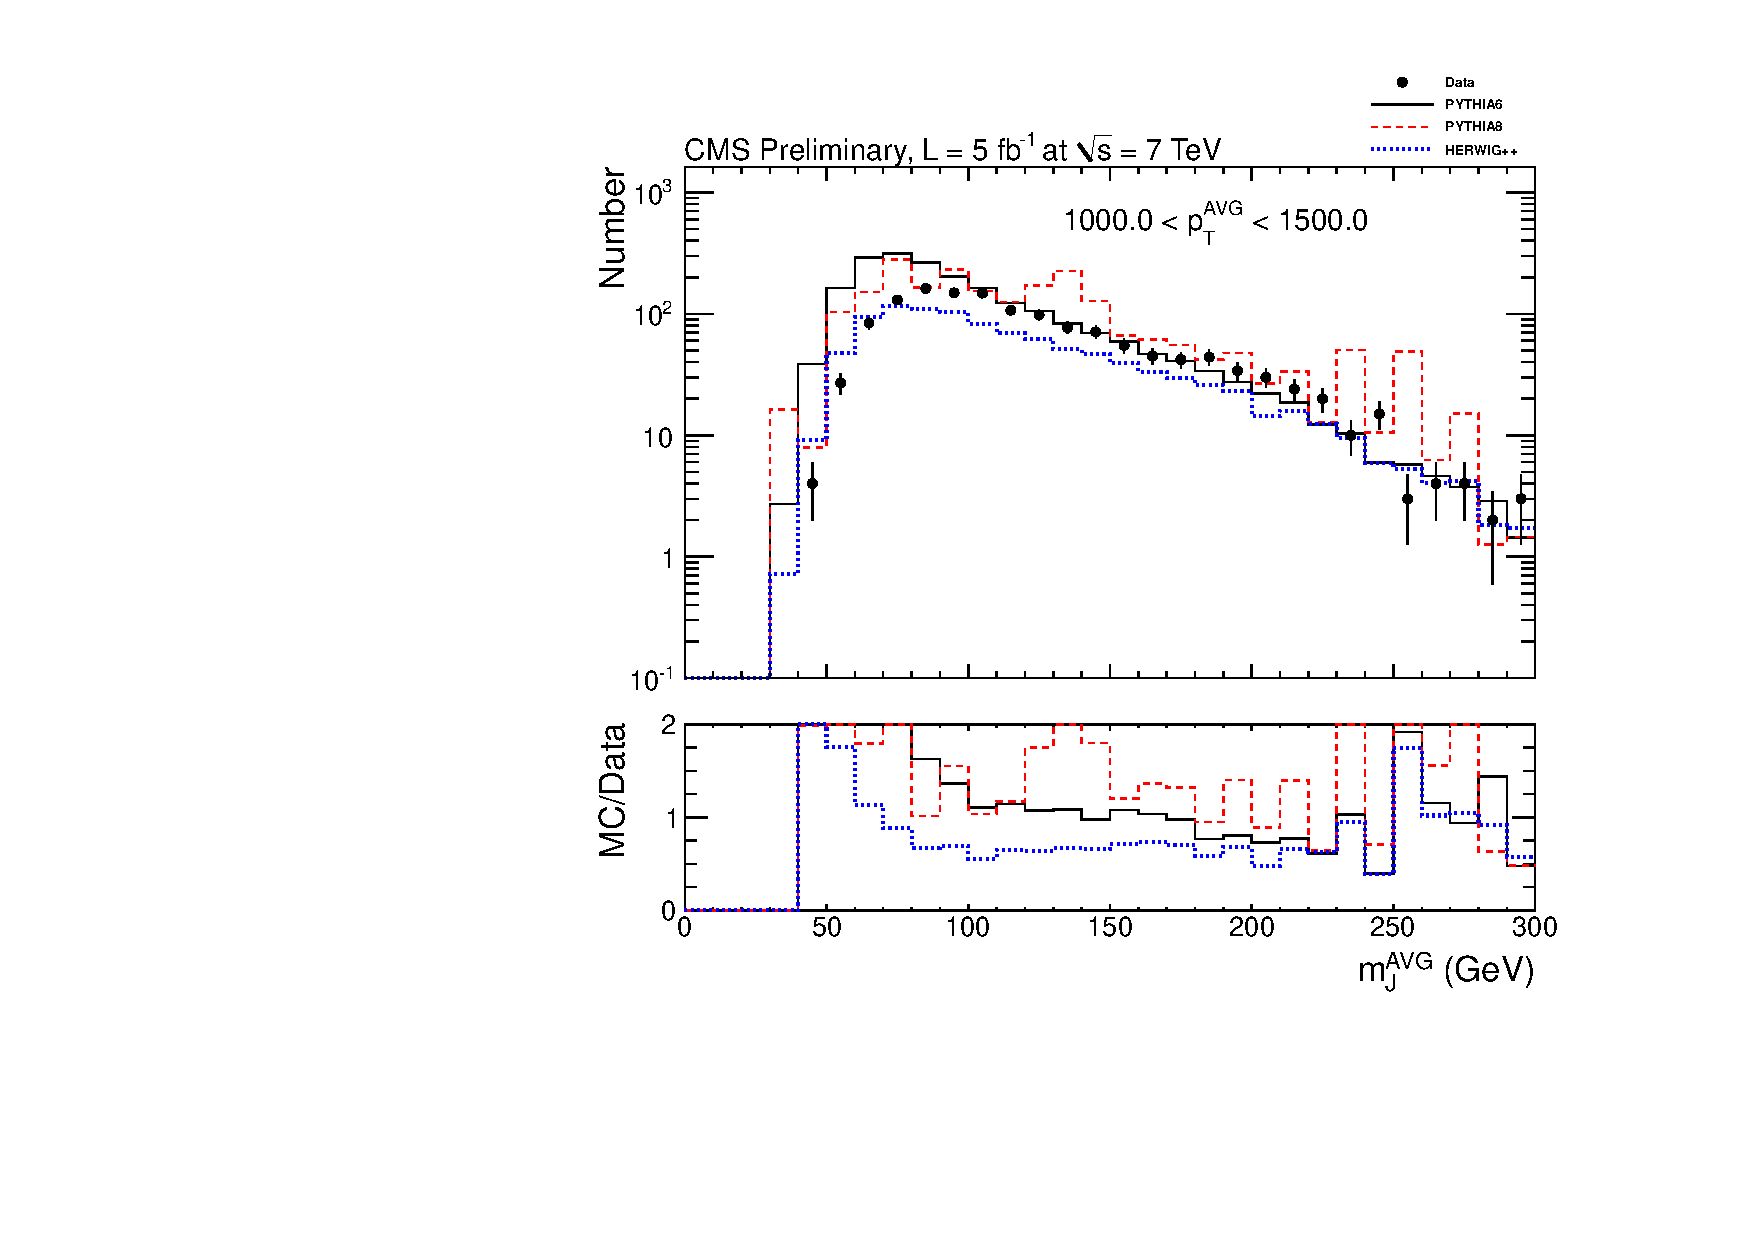
\includegraphics[width=0.95\textwidth]{figs/histAK7MjetVsPtAvg_rawDataMCComparisons_pt_10_Filtered}
\caption{Detector-level distributions of the jet mass for AK7 Filtered jets,
for $1000.0 < \pt^{AVG} < 1500.0$ \GeVc. The data are shown in black points.
The simulated distribution from \PYTHIA is shown in solid black, 
the from \PYTHIAEIGHT in dashed red, and from \HERWIG in dotted blue. 
The bottom frame shows the ratio of the simulated distribution
to the distribution from data. 
\label{figs:histAK7MjetVsPtAvg_rawDataMCComparisons_pt_10_Filtered}}
\end{figure}


\clearpage



\begin{figure}[htbp]
\centering
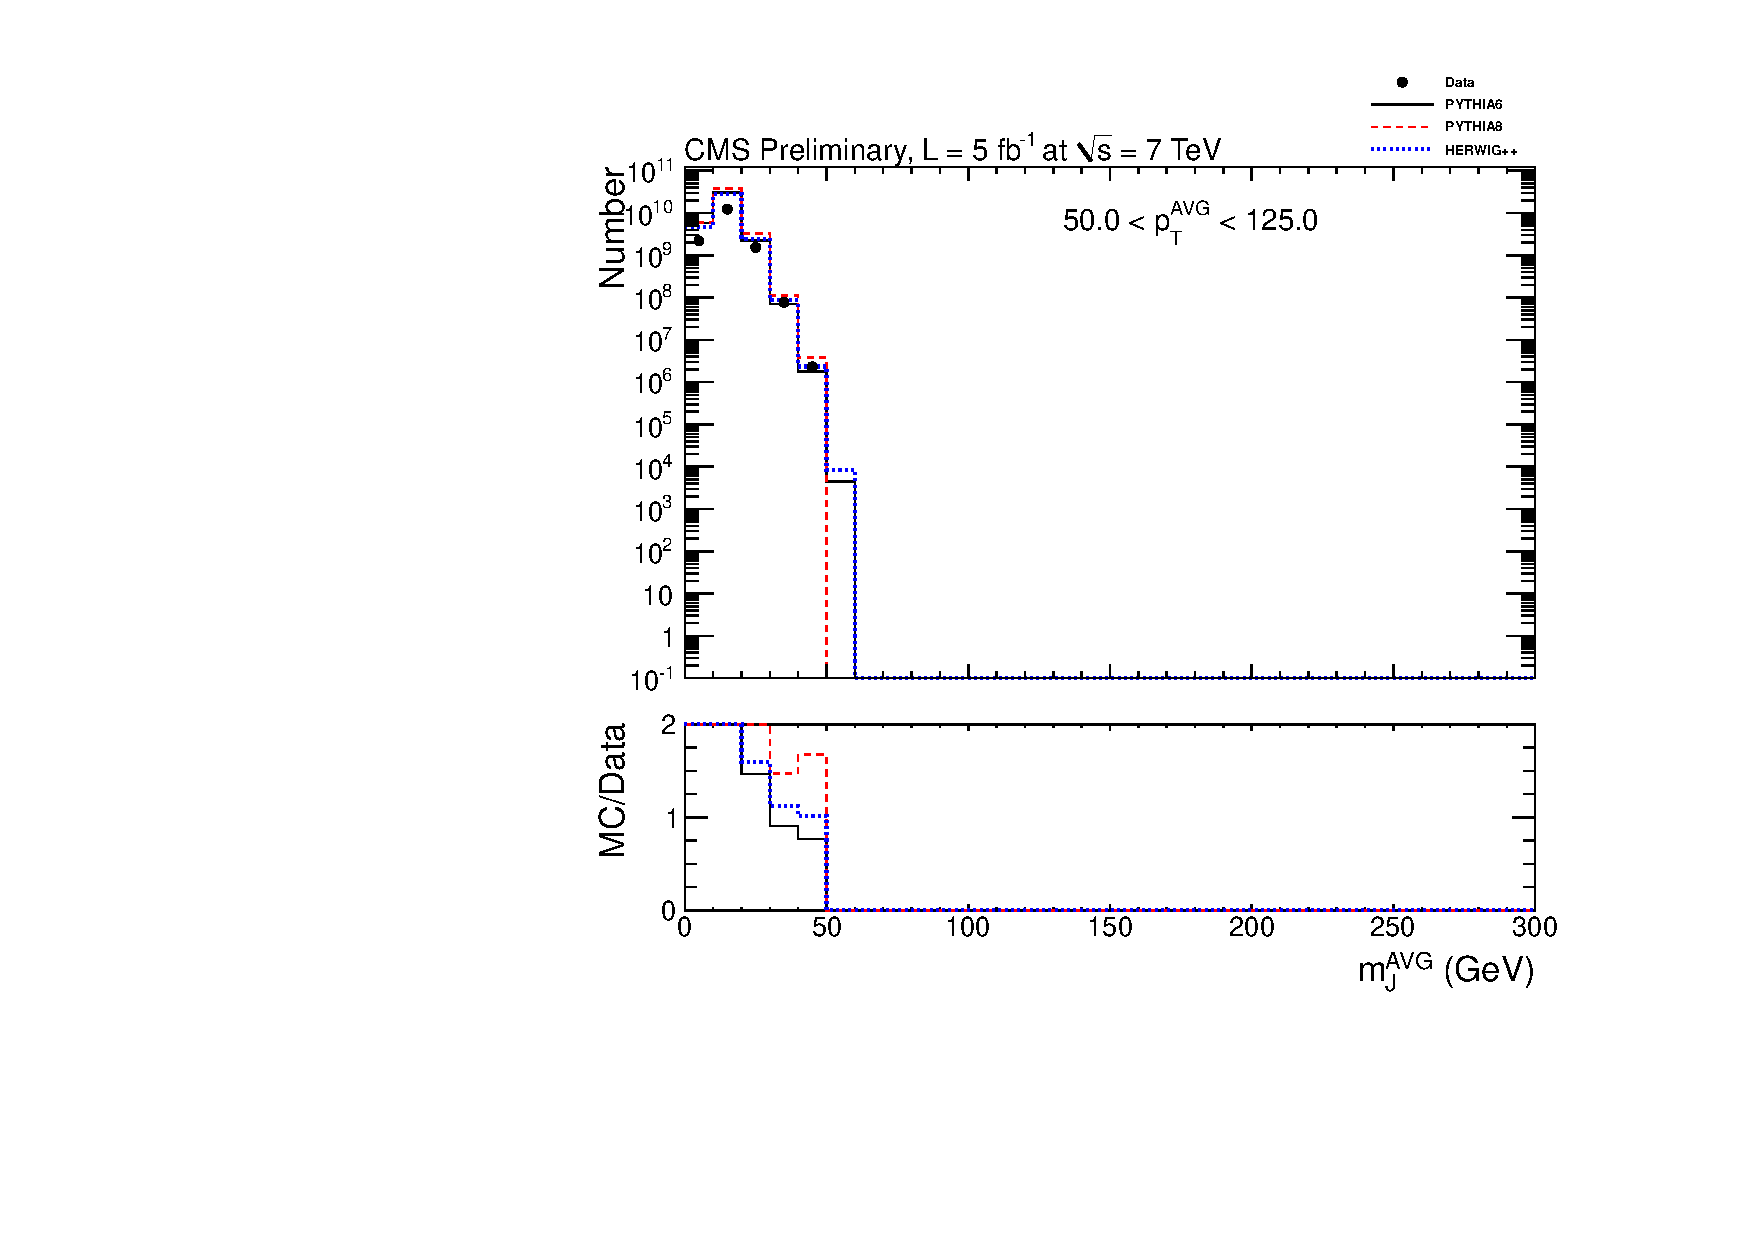
\includegraphics[width=0.95\textwidth]{figs/histAK7MjetVsPtAvg_rawDataMCComparisons_pt_1_Trimmed}
\caption{Detector-level distributions of the jet mass for AK7 Trimmed jets,
for $50.0 < \pt^{AVG} < 125.0$ \GeVc. The data are shown in black points.
The simulated distribution from \PYTHIA is shown in solid black, 
the from \PYTHIAEIGHT in dashed red, and from \HERWIG in dotted blue. 
The bottom frame shows the ratio of the simulated distribution
to the distribution from data. 
\label{figs:histAK7MjetVsPtAvg_rawDataMCComparisons_pt_1_Trimmed}}
\end{figure}



\begin{figure}[htbp]
\centering
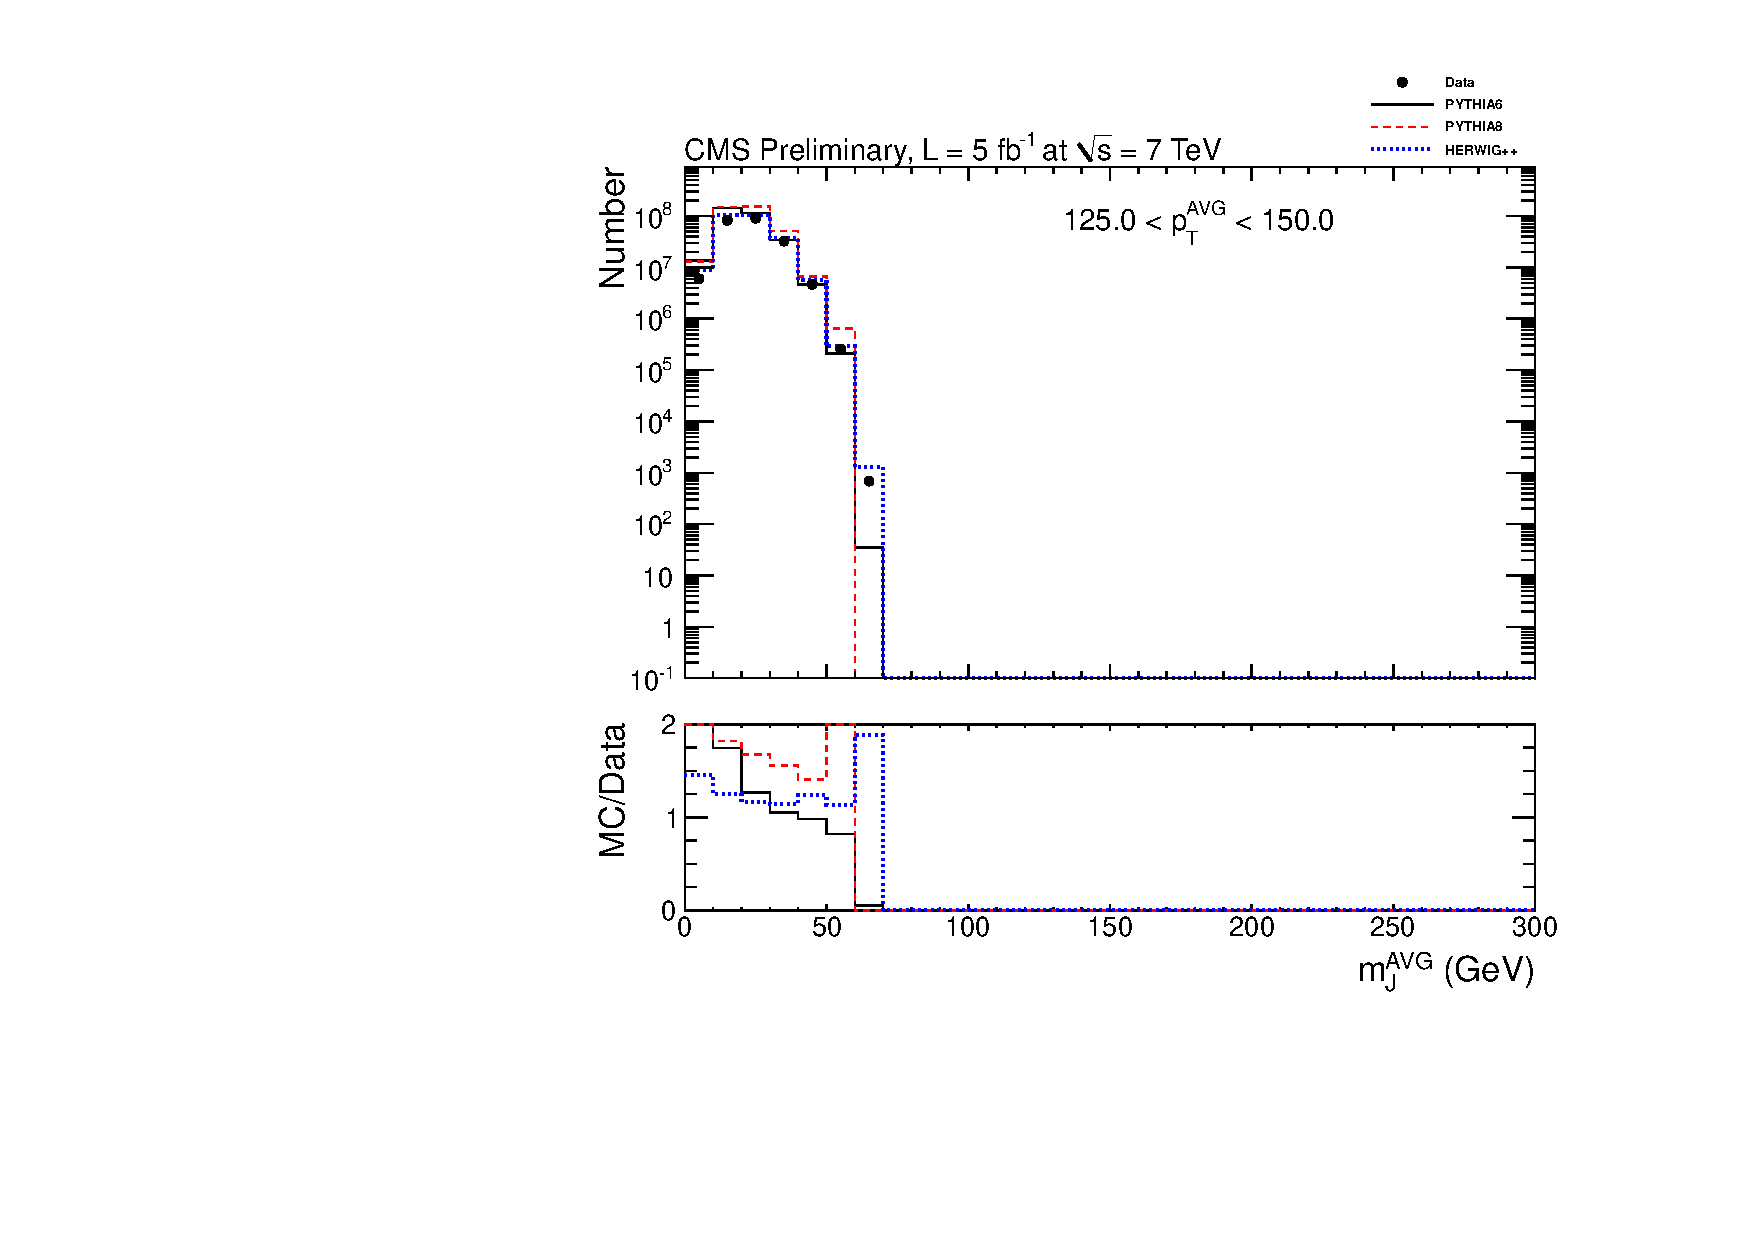
\includegraphics[width=0.95\textwidth]{figs/histAK7MjetVsPtAvg_rawDataMCComparisons_pt_2_Trimmed}
\caption{Detector-level distributions of the jet mass for AK7 Trimmed jets,
for $125.0 < \pt^{AVG} < 150.0$ \GeVc. The data are shown in black points.
The simulated distribution from \PYTHIA is shown in solid black, 
the from \PYTHIAEIGHT in dashed red, and from \HERWIG in dotted blue. 
The bottom frame shows the ratio of the simulated distribution
to the distribution from data. 
\label{figs:histAK7MjetVsPtAvg_rawDataMCComparisons_pt_2_Trimmed}}
\end{figure}



\begin{figure}[htbp]
\centering
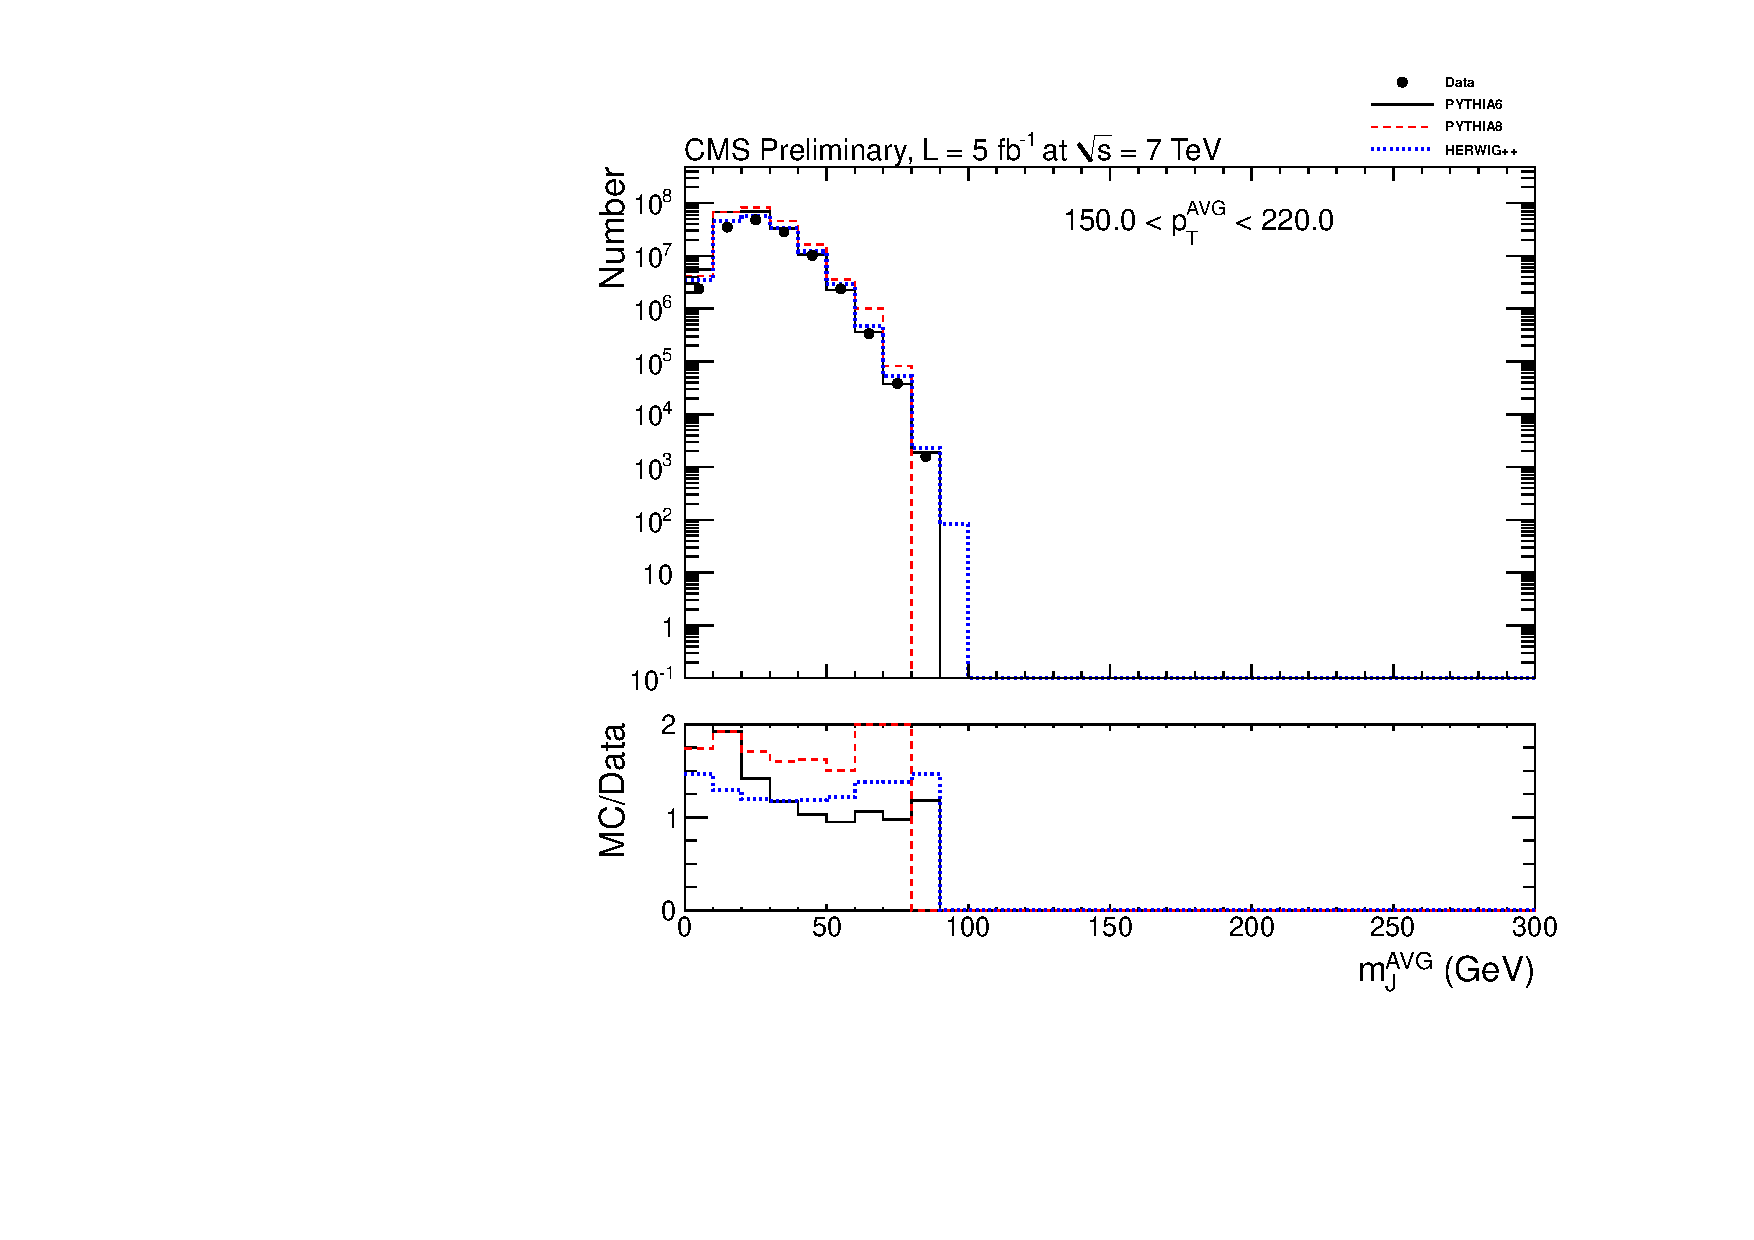
\includegraphics[width=0.95\textwidth]{figs/histAK7MjetVsPtAvg_rawDataMCComparisons_pt_3_Trimmed}
\caption{Detector-level distributions of the jet mass for AK7 Trimmed jets,
for $150.0 < \pt^{AVG} < 220.0$ \GeVc. The data are shown in black points.
The simulated distribution from \PYTHIA is shown in solid black, 
the from \PYTHIAEIGHT in dashed red, and from \HERWIG in dotted blue. 
The bottom frame shows the ratio of the simulated distribution
to the distribution from data. 
\label{figs:histAK7MjetVsPtAvg_rawDataMCComparisons_pt_3_Trimmed}}
\end{figure}



\begin{figure}[htbp]
\centering
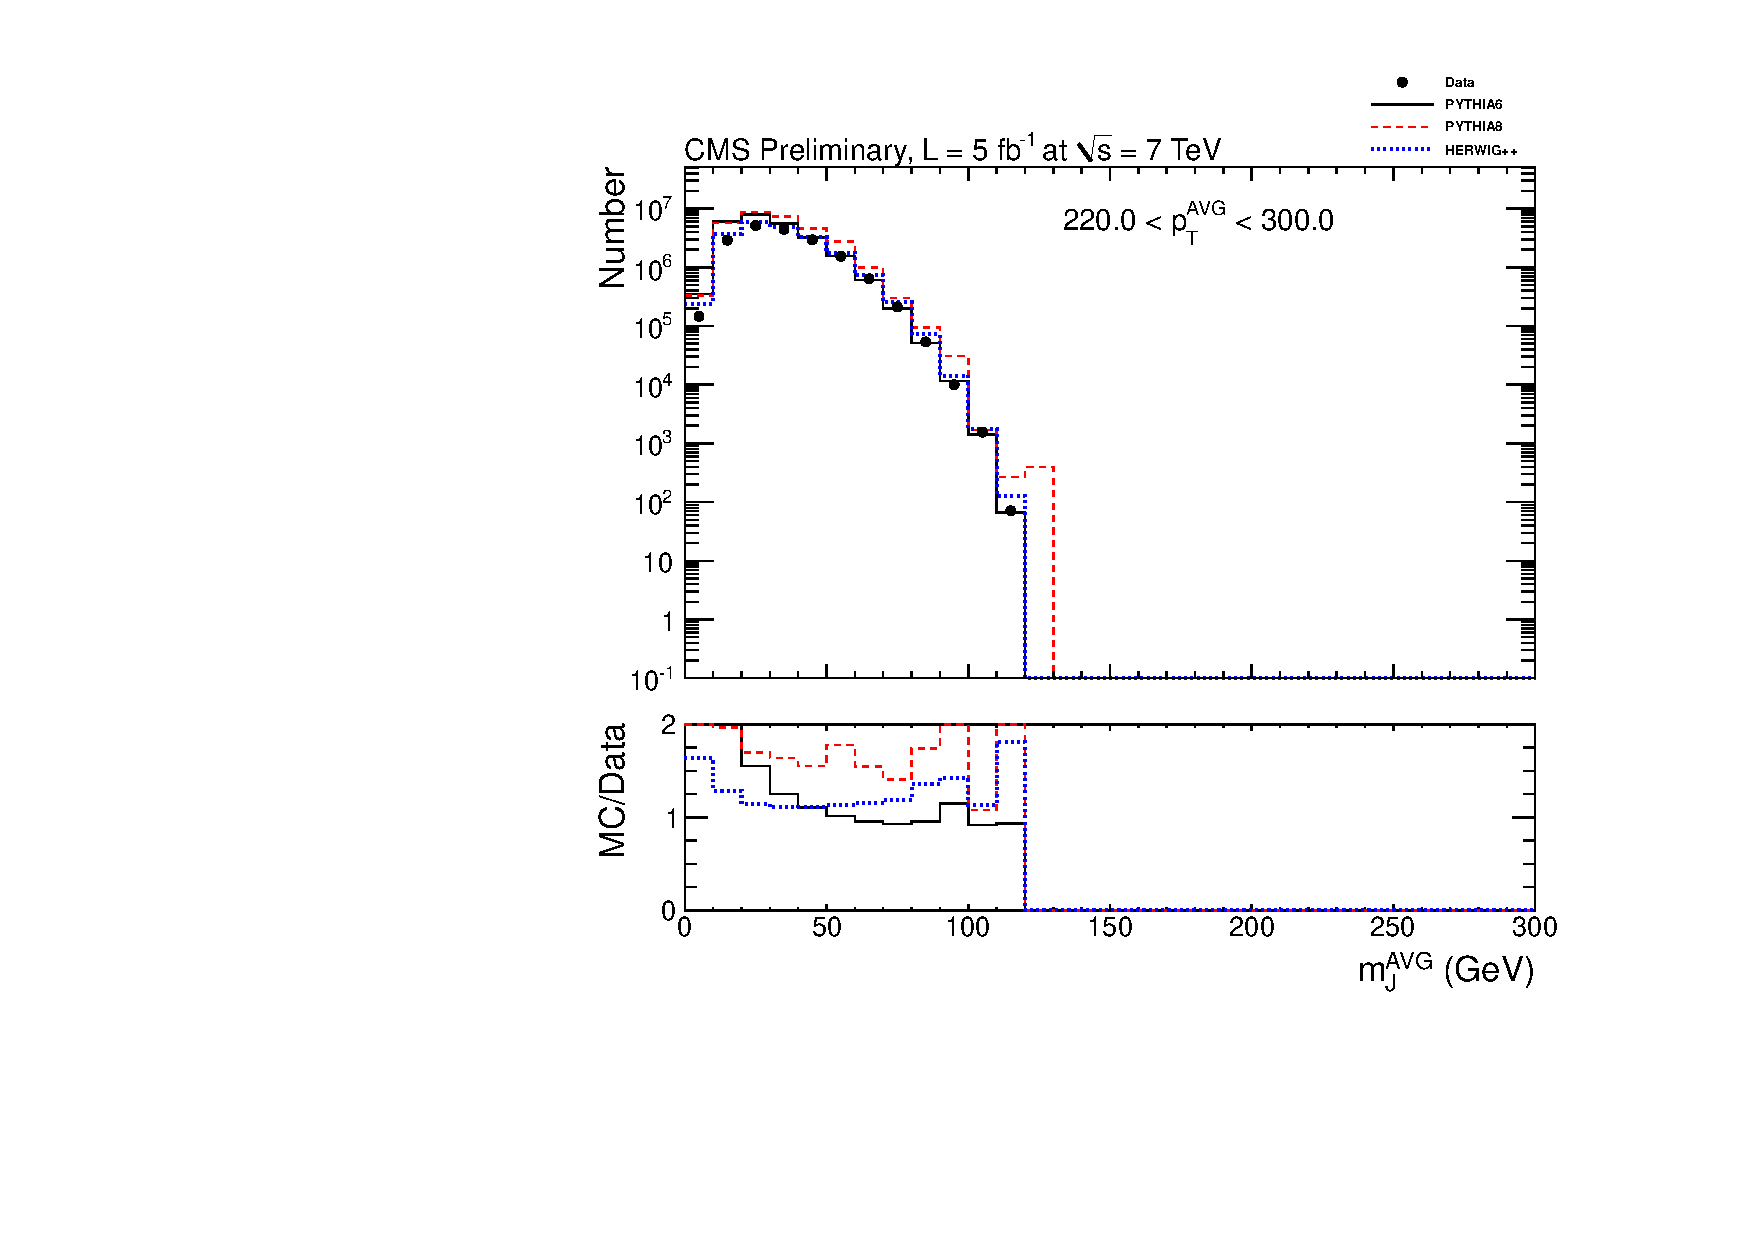
\includegraphics[width=0.95\textwidth]{figs/histAK7MjetVsPtAvg_rawDataMCComparisons_pt_4_Trimmed}
\caption{Detector-level distributions of the jet mass for AK7 Trimmed jets,
for $220.0 < \pt^{AVG} < 300.0$ \GeVc. The data are shown in black points.
The simulated distribution from \PYTHIA is shown in solid black, 
the from \PYTHIAEIGHT in dashed red, and from \HERWIG in dotted blue. 
The bottom frame shows the ratio of the simulated distribution
to the distribution from data. 
\label{figs:histAK7MjetVsPtAvg_rawDataMCComparisons_pt_4_Trimmed}}
\end{figure}



\begin{figure}[htbp]
\centering
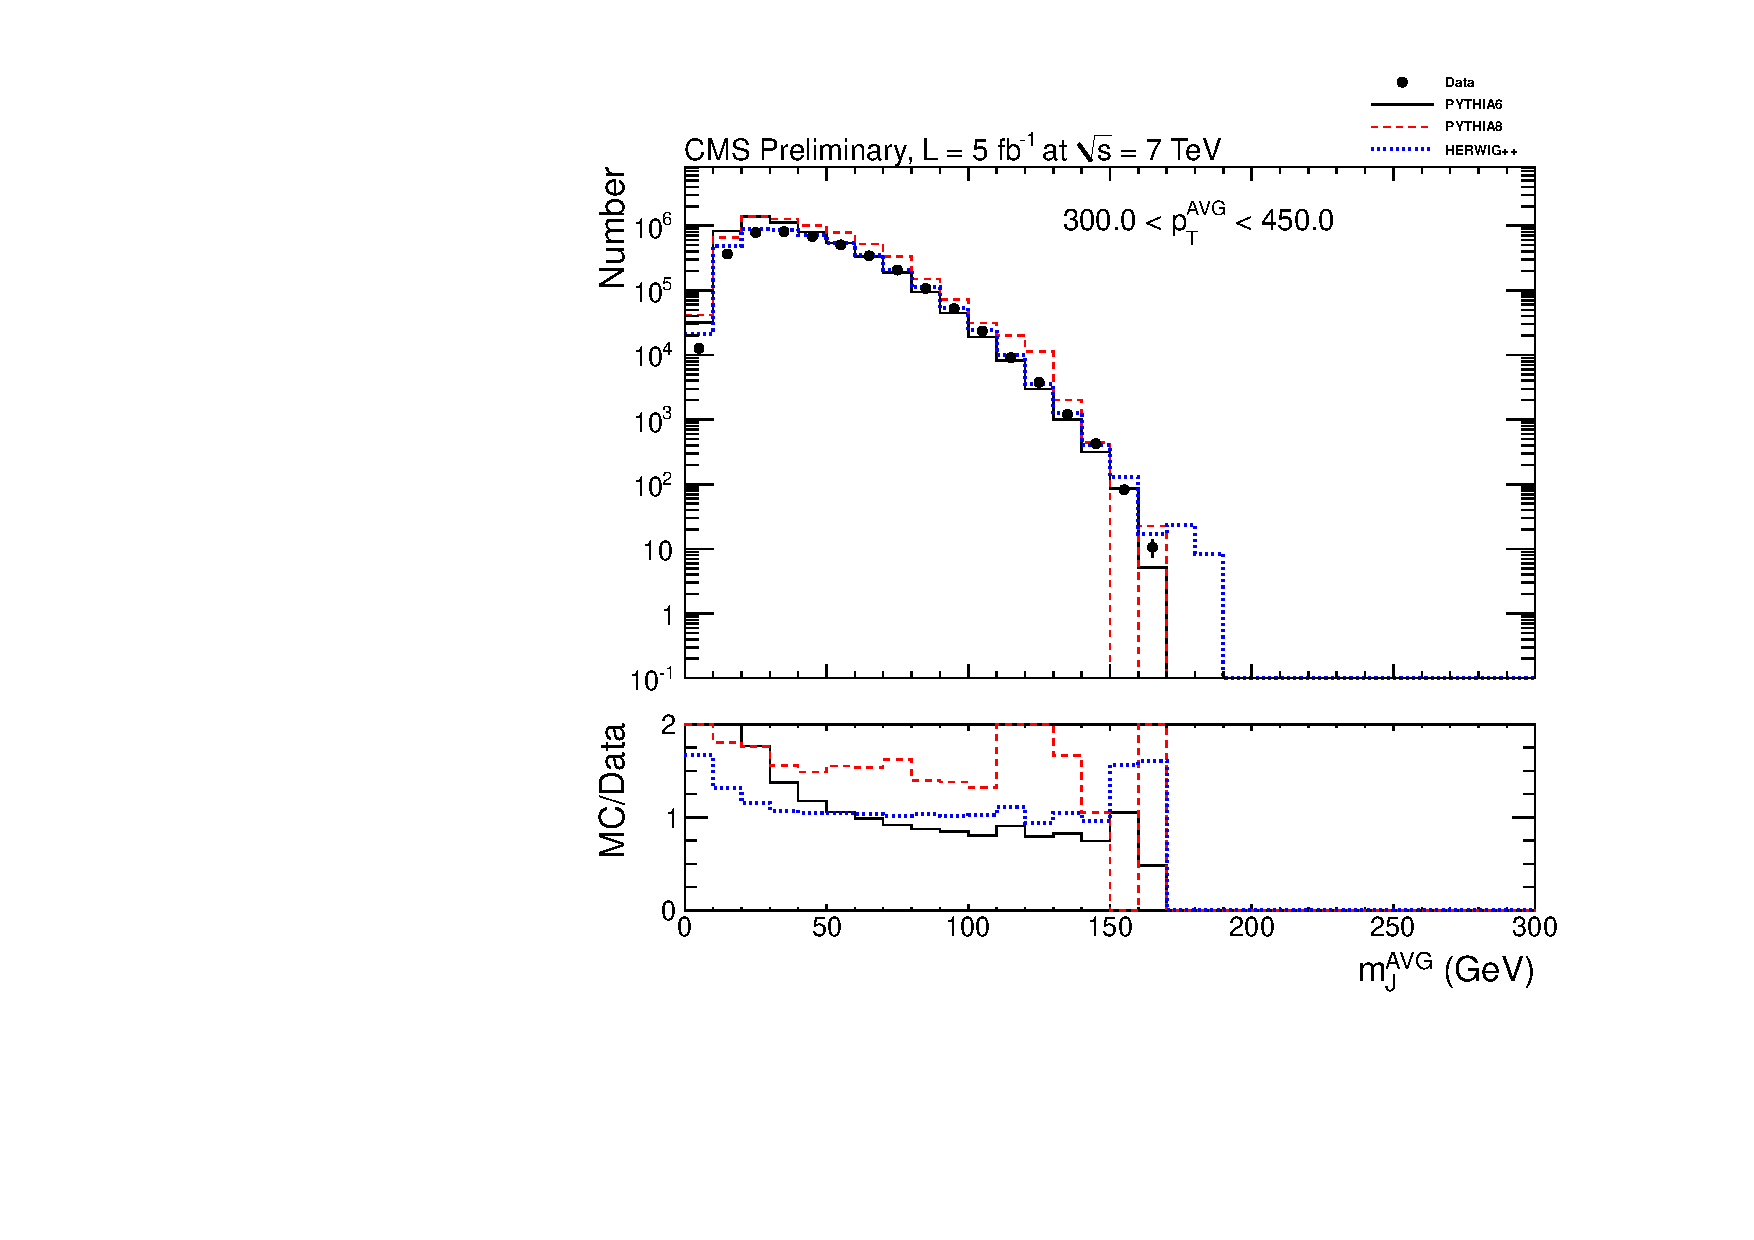
\includegraphics[width=0.95\textwidth]{figs/histAK7MjetVsPtAvg_rawDataMCComparisons_pt_5_Trimmed}
\caption{Detector-level distributions of the jet mass for AK7 Trimmed jets,
for $300.0 < \pt^{AVG} < 450.0$ \GeVc. The data are shown in black points.
The simulated distribution from \PYTHIA is shown in solid black, 
the from \PYTHIAEIGHT in dashed red, and from \HERWIG in dotted blue. 
The bottom frame shows the ratio of the simulated distribution
to the distribution from data. 
\label{figs:histAK7MjetVsPtAvg_rawDataMCComparisons_pt_5_Trimmed}}
\end{figure}



\begin{figure}[htbp]
\centering
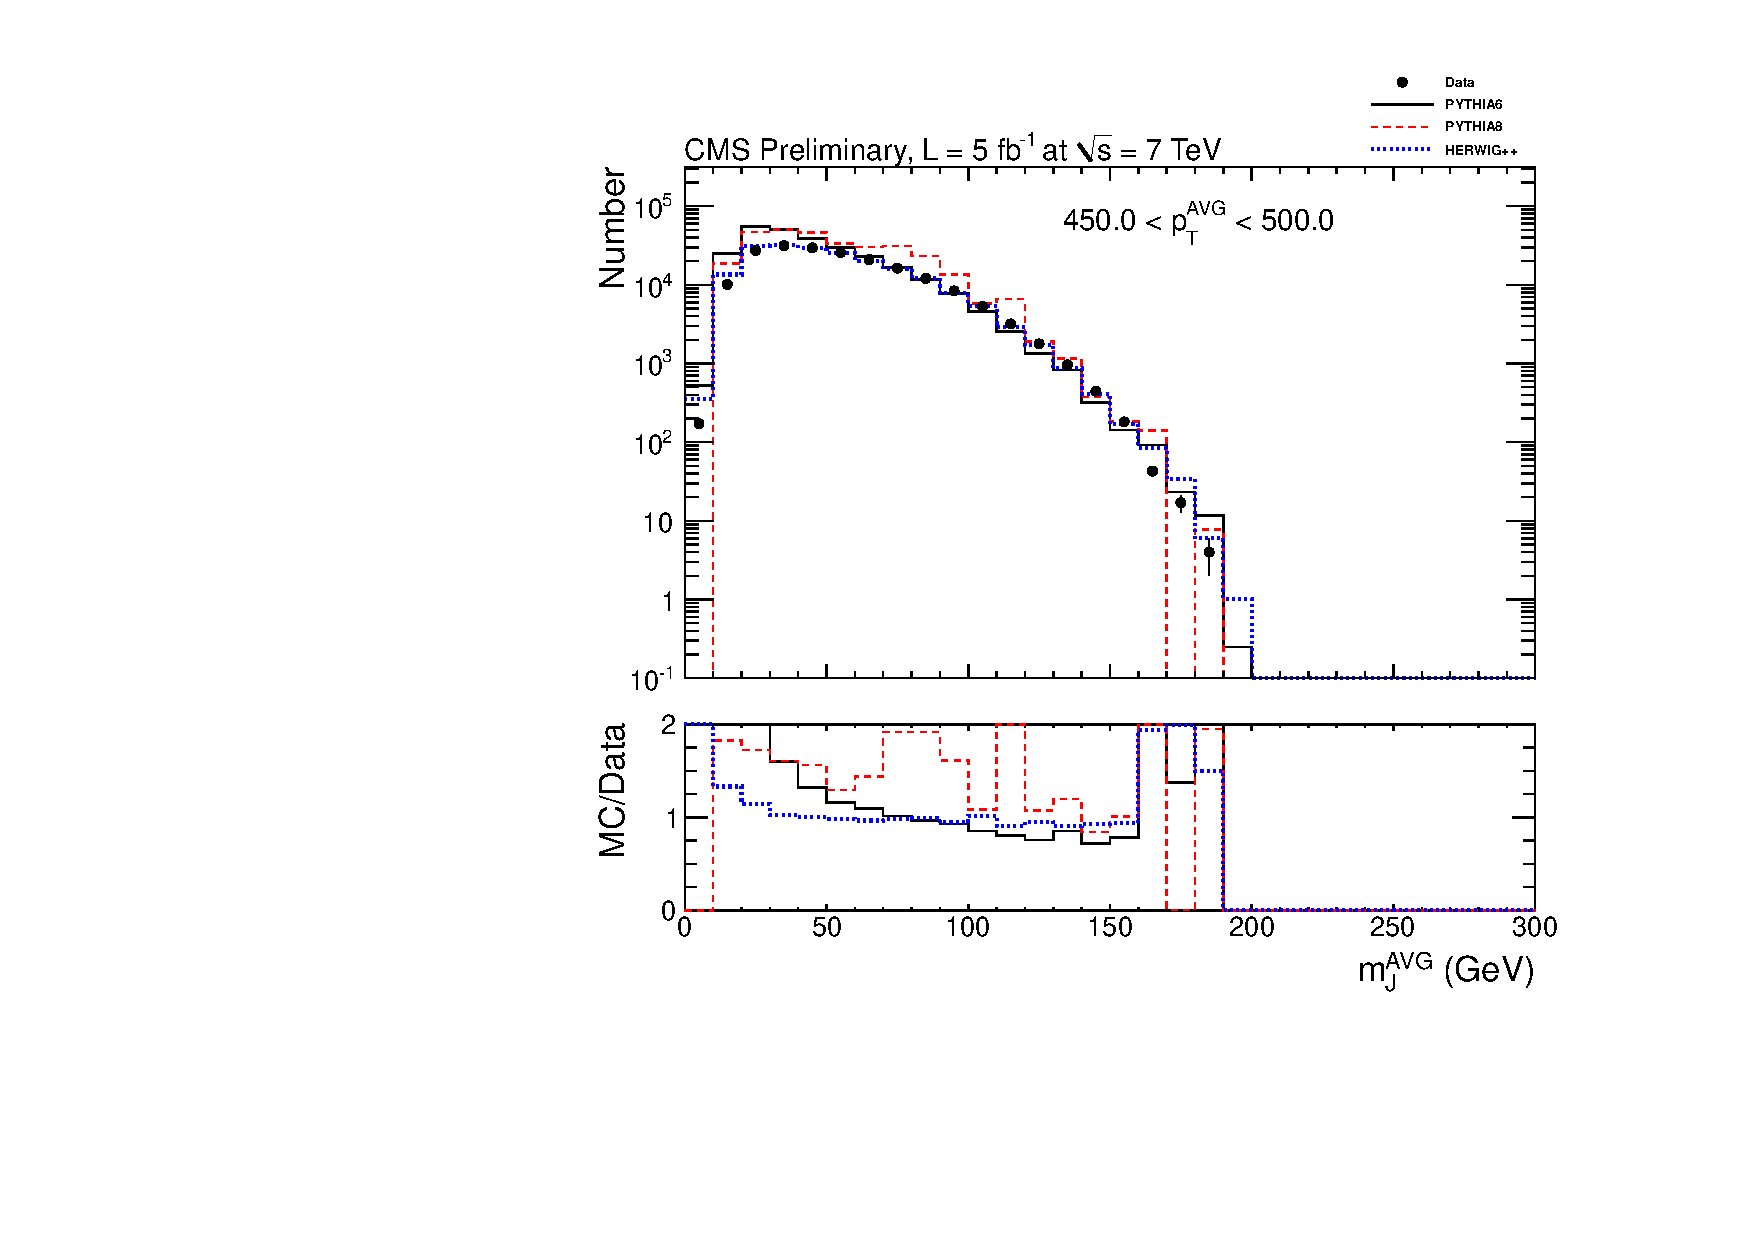
\includegraphics[width=0.95\textwidth]{figs/histAK7MjetVsPtAvg_rawDataMCComparisons_pt_6_Trimmed}
\caption{Detector-level distributions of the jet mass for AK7 Trimmed jets,
for $450.0 < \pt^{AVG} < 500.0$ \GeVc. The data are shown in black points.
The simulated distribution from \PYTHIA is shown in solid black, 
the from \PYTHIAEIGHT in dashed red, and from \HERWIG in dotted blue. 
The bottom frame shows the ratio of the simulated distribution
to the distribution from data. 
\label{figs:histAK7MjetVsPtAvg_rawDataMCComparisons_pt_6_Trimmed}}
\end{figure}



\begin{figure}[htbp]
\centering
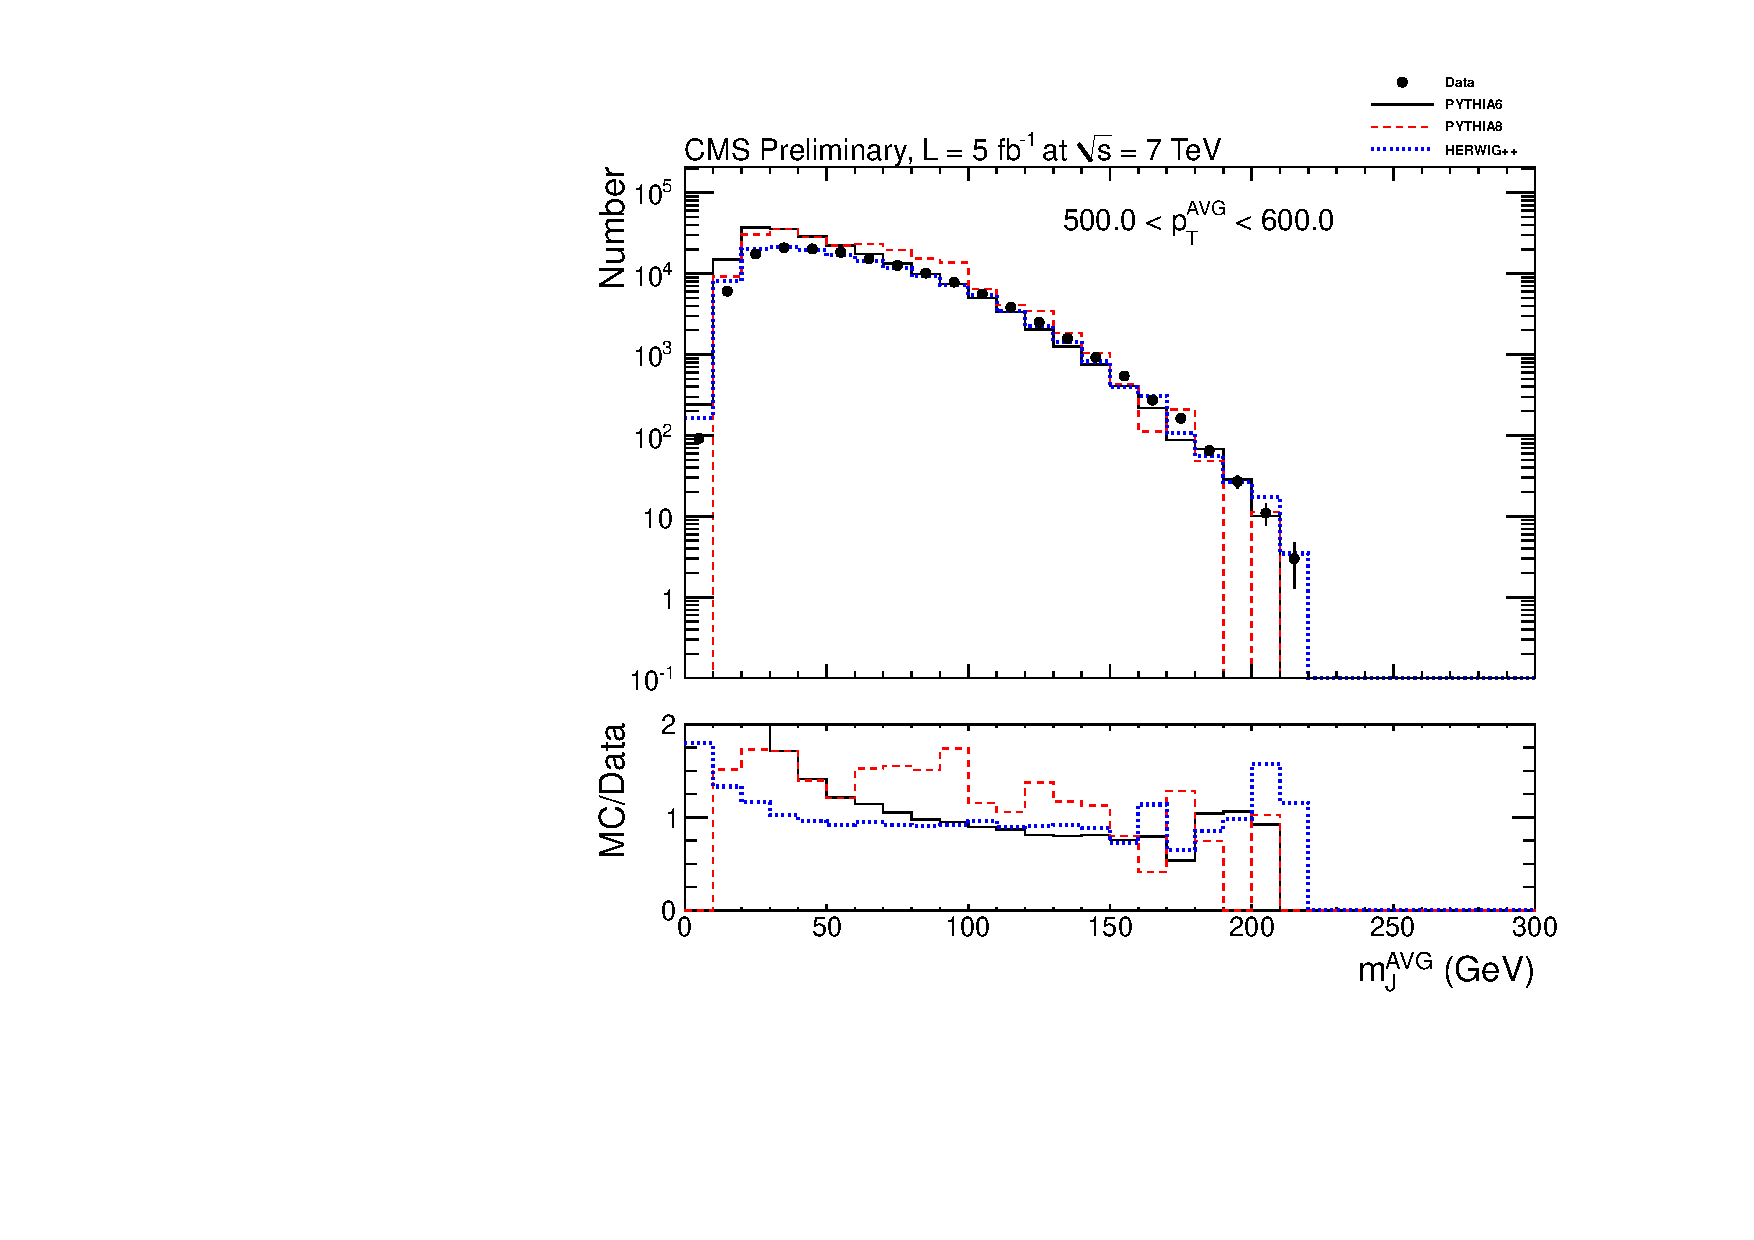
\includegraphics[width=0.95\textwidth]{figs/histAK7MjetVsPtAvg_rawDataMCComparisons_pt_7_Trimmed}
\caption{Detector-level distributions of the jet mass for AK7 Trimmed jets,
for $500.0 < \pt^{AVG} < 600.0$ \GeVc. The data are shown in black points.
The simulated distribution from \PYTHIA is shown in solid black, 
the from \PYTHIAEIGHT in dashed red, and from \HERWIG in dotted blue. 
The bottom frame shows the ratio of the simulated distribution
to the distribution from data. 
\label{figs:histAK7MjetVsPtAvg_rawDataMCComparisons_pt_7_Trimmed}}
\end{figure}



\begin{figure}[htbp]
\centering
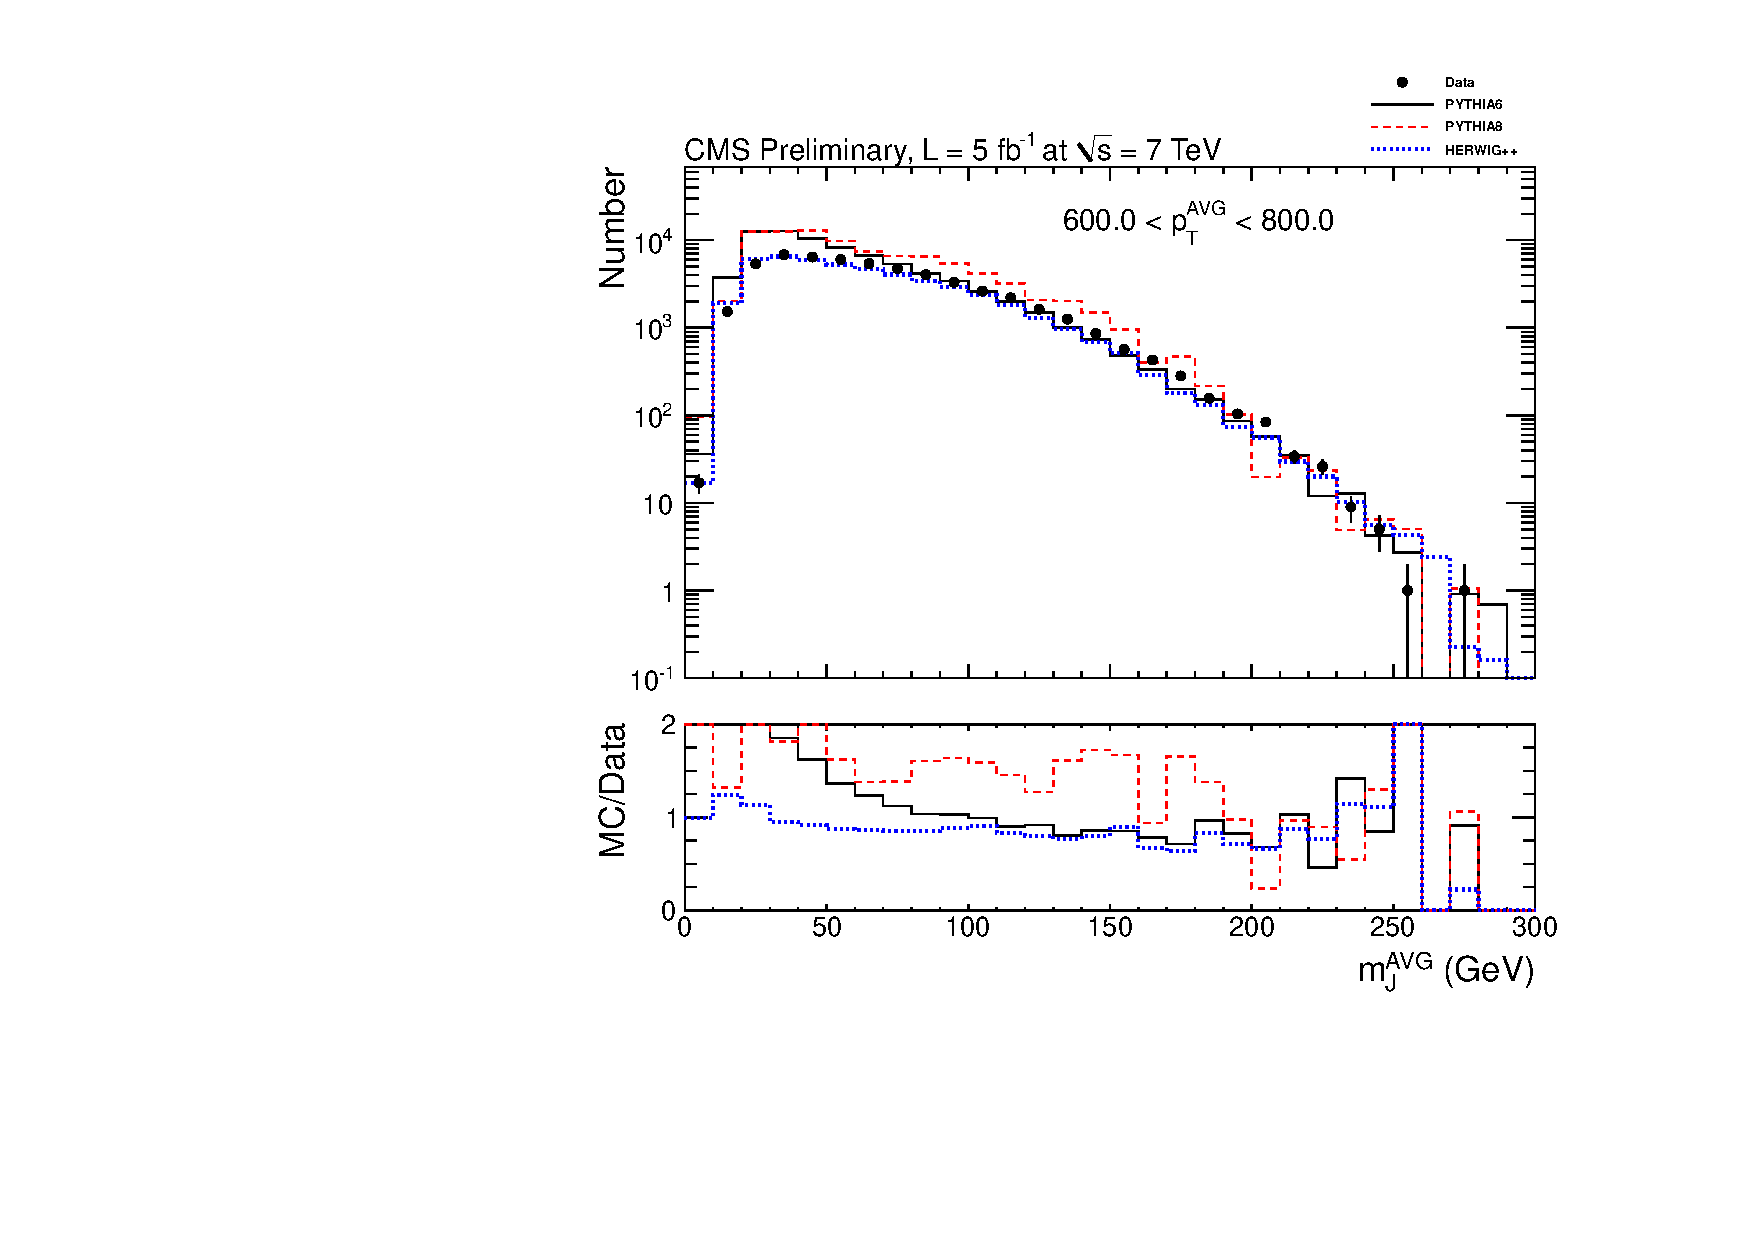
\includegraphics[width=0.95\textwidth]{figs/histAK7MjetVsPtAvg_rawDataMCComparisons_pt_8_Trimmed}
\caption{Detector-level distributions of the jet mass for AK7 Trimmed jets,
for $600.0 < \pt^{AVG} < 800.0$ \GeVc. The data are shown in black points.
The simulated distribution from \PYTHIA is shown in solid black, 
the from \PYTHIAEIGHT in dashed red, and from \HERWIG in dotted blue. 
The bottom frame shows the ratio of the simulated distribution
to the distribution from data. 
\label{figs:histAK7MjetVsPtAvg_rawDataMCComparisons_pt_8_Trimmed}}
\end{figure}



\begin{figure}[htbp]
\centering
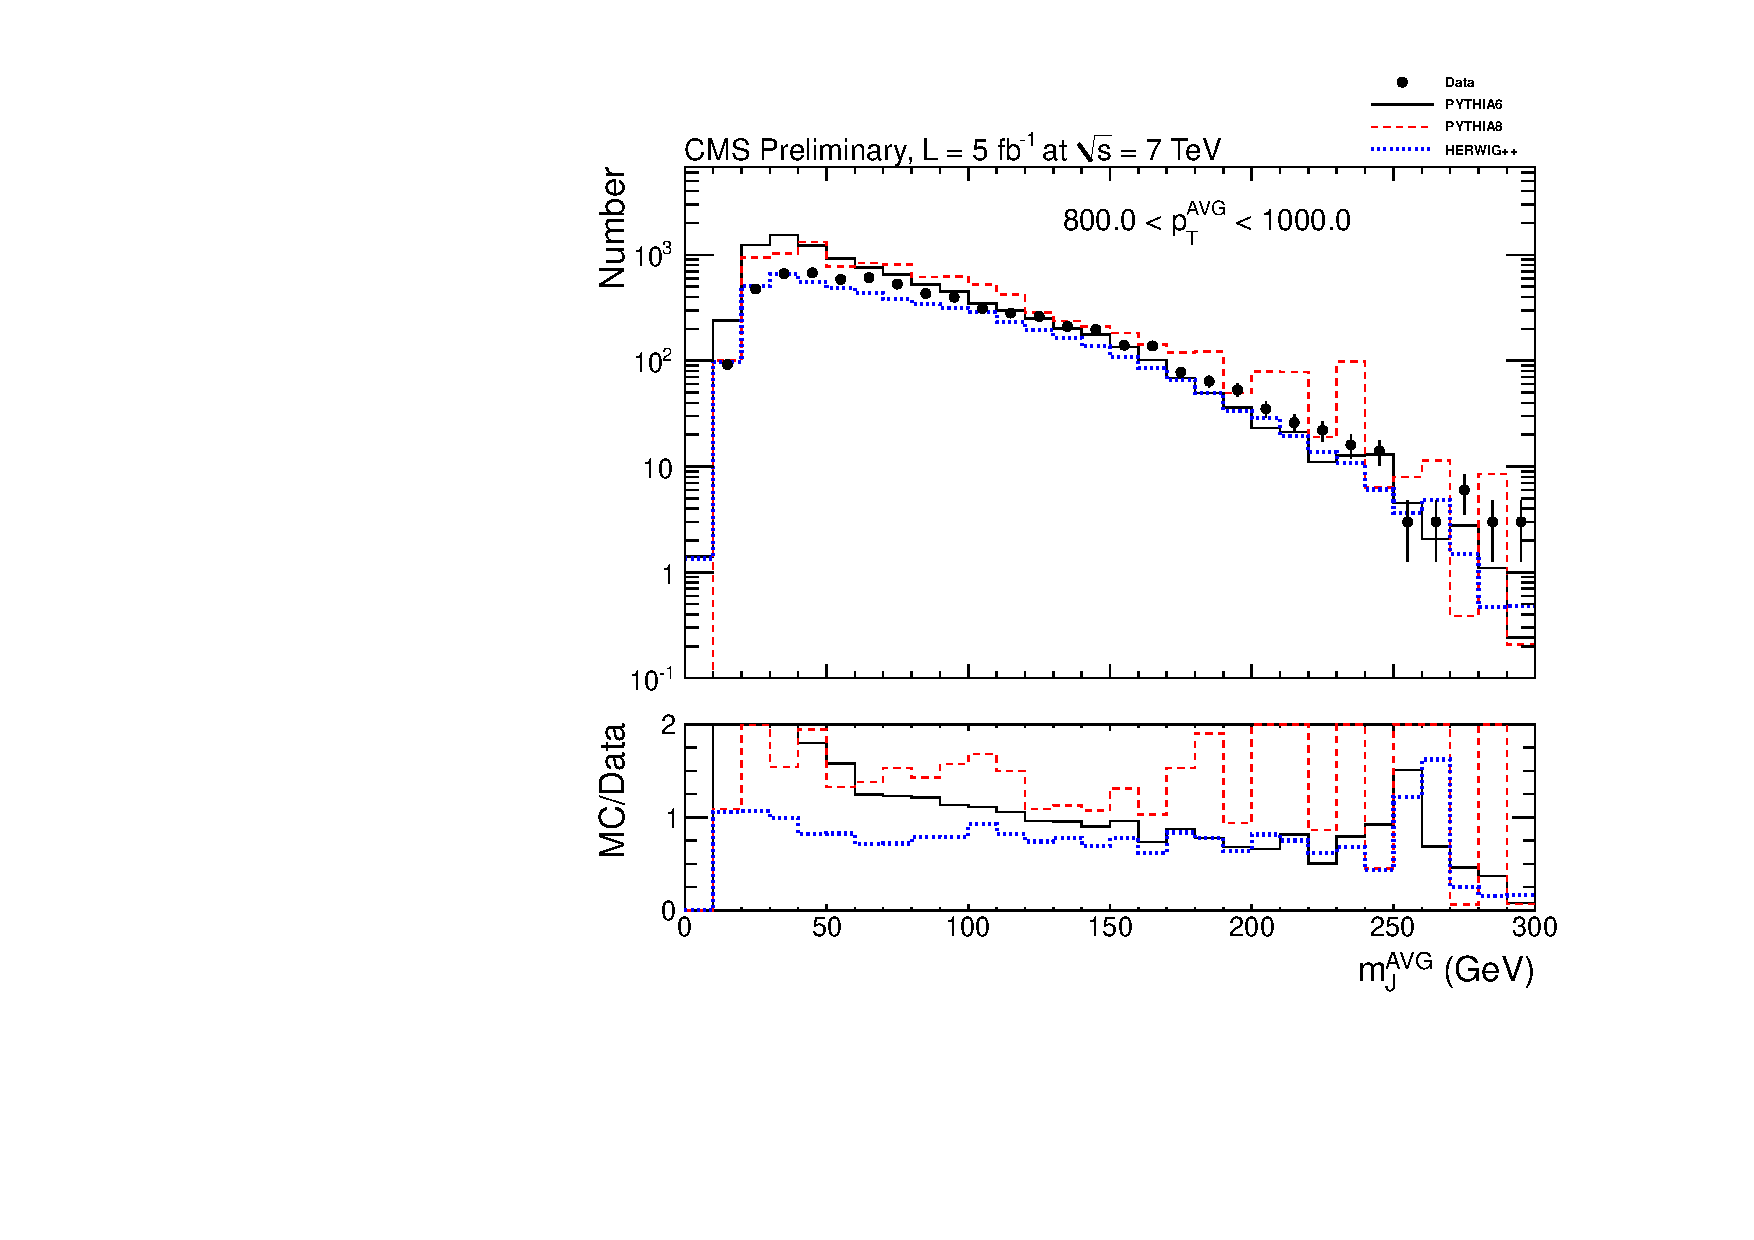
\includegraphics[width=0.95\textwidth]{figs/histAK7MjetVsPtAvg_rawDataMCComparisons_pt_9_Trimmed}
\caption{Detector-level distributions of the jet mass for AK7 Trimmed jets,
for $800.0 < \pt^{AVG} < 1000.0$ \GeVc. The data are shown in black points.
The simulated distribution from \PYTHIA is shown in solid black, 
the from \PYTHIAEIGHT in dashed red, and from \HERWIG in dotted blue. 
The bottom frame shows the ratio of the simulated distribution
to the distribution from data. 
\label{figs:histAK7MjetVsPtAvg_rawDataMCComparisons_pt_9_Trimmed}}
\end{figure}



\begin{figure}[htbp]
\centering
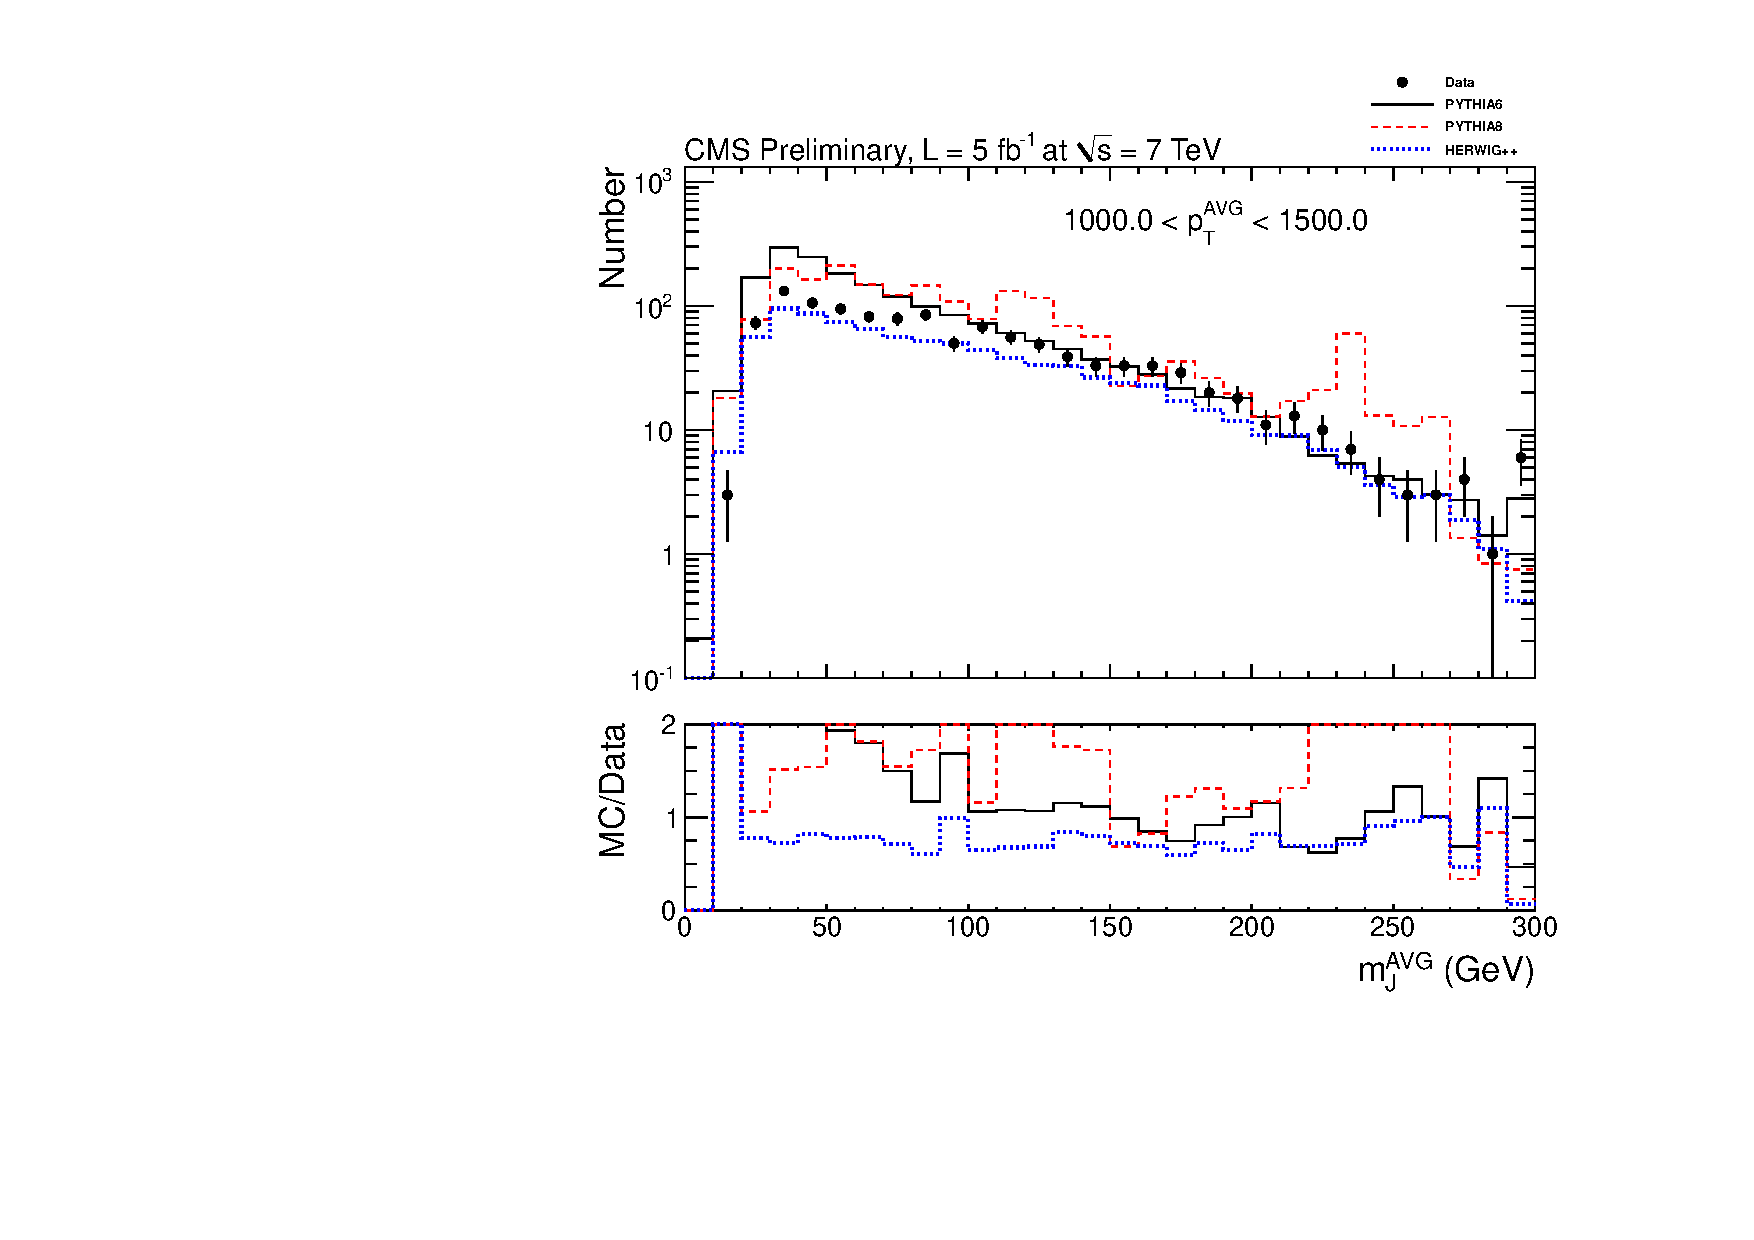
\includegraphics[width=0.95\textwidth]{figs/histAK7MjetVsPtAvg_rawDataMCComparisons_pt_10_Trimmed}
\caption{Detector-level distributions of the jet mass for AK7 Trimmed jets,
for $1000.0 < \pt^{AVG} < 1500.0$ \GeVc. The data are shown in black points.
The simulated distribution from \PYTHIA is shown in solid black, 
the from \PYTHIAEIGHT in dashed red, and from \HERWIG in dotted blue. 
The bottom frame shows the ratio of the simulated distribution
to the distribution from data. 
\label{figs:histAK7MjetVsPtAvg_rawDataMCComparisons_pt_10_Trimmed}}
\end{figure}


\clearpage



\begin{figure}[htbp]
\centering
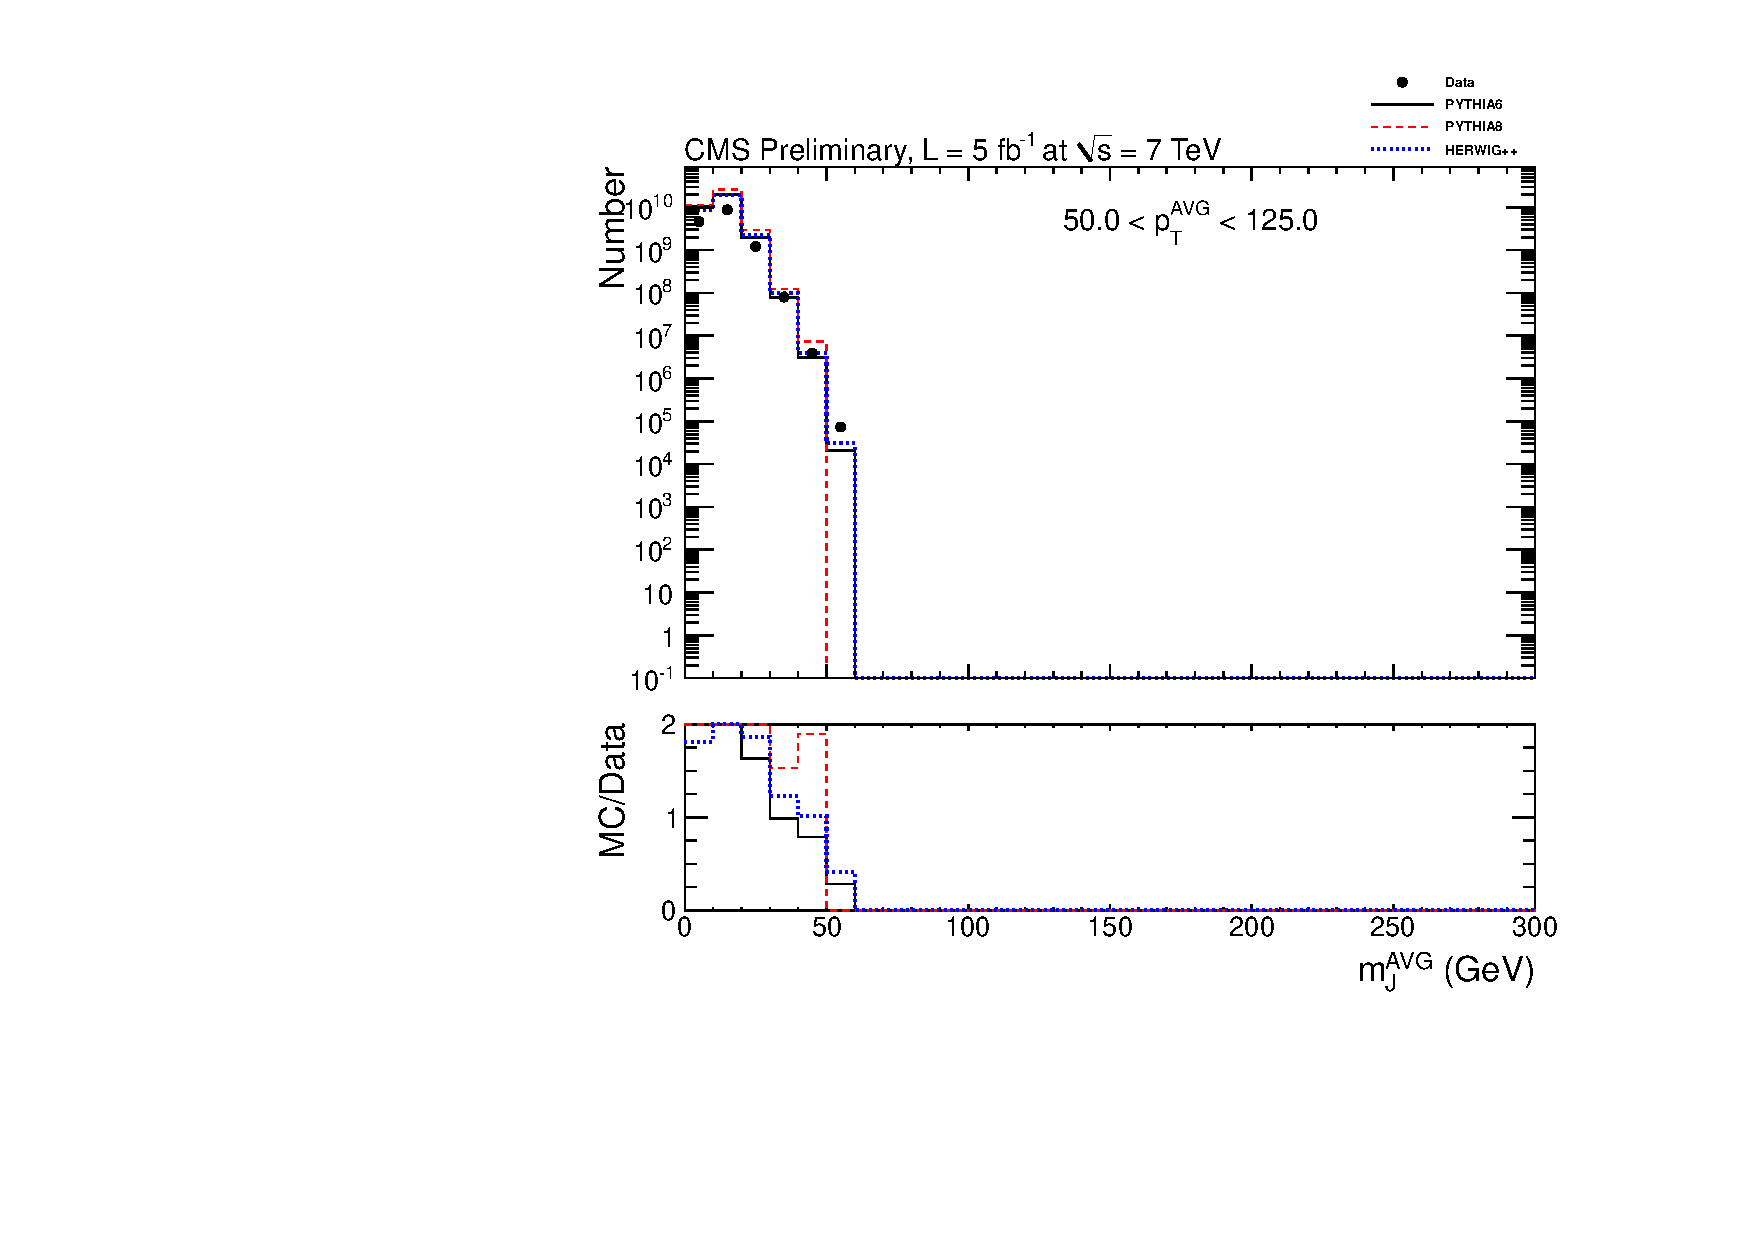
\includegraphics[width=0.95\textwidth]{figs/histAK7MjetVsPtAvg_rawDataMCComparisons_pt_1_Pruned}
\caption{Detector-level distributions of the jet mass for AK7 Pruned jets,
for $50.0 < \pt^{AVG} < 125.0$ \GeVc. The data are shown in black points.
The simulated distribution from \PYTHIA is shown in solid black, 
the from \PYTHIAEIGHT in dashed red, and from \HERWIG in dotted blue. 
The bottom frame shows the ratio of the simulated distribution
to the distribution from data. 
\label{figs:histAK7MjetVsPtAvg_rawDataMCComparisons_pt_1_Pruned}}
\end{figure}



\begin{figure}[htbp]
\centering
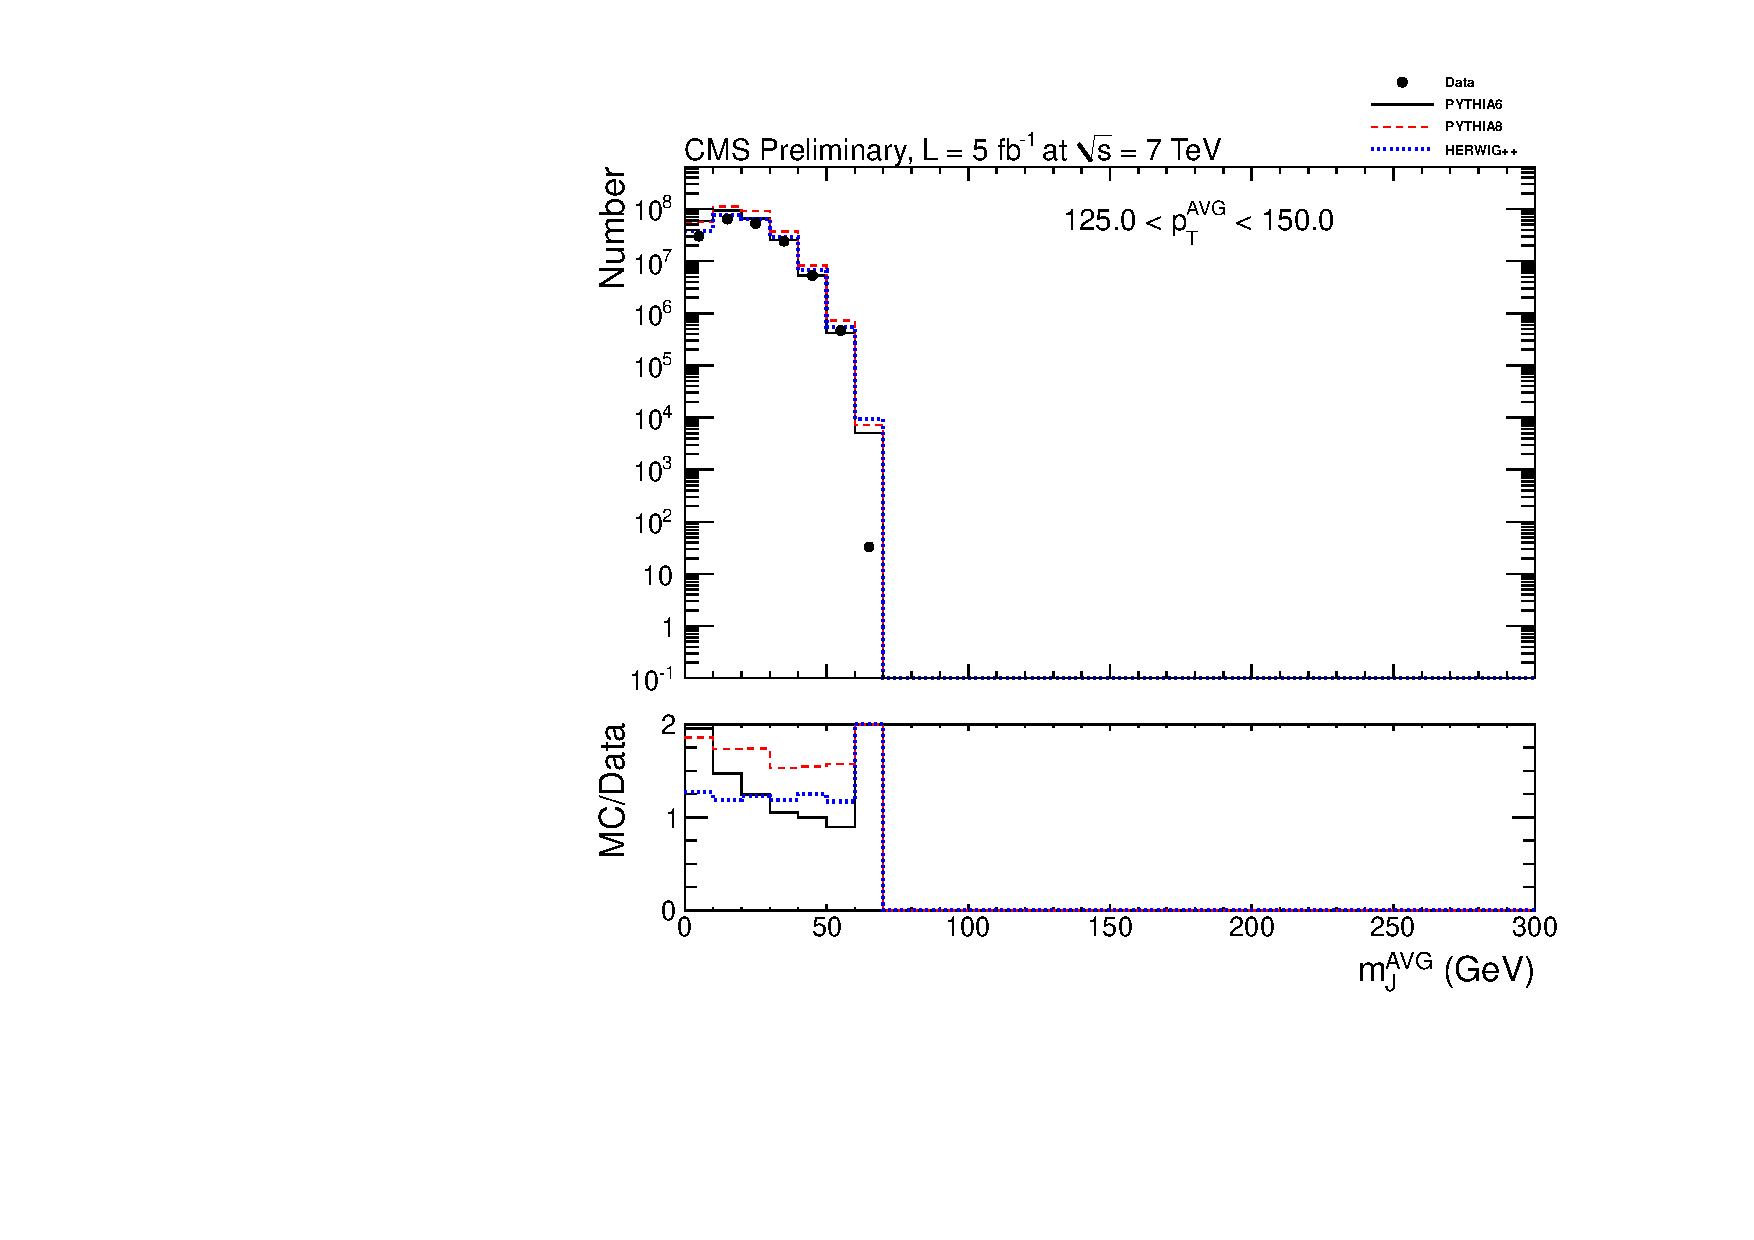
\includegraphics[width=0.95\textwidth]{figs/histAK7MjetVsPtAvg_rawDataMCComparisons_pt_2_Pruned}
\caption{Detector-level distributions of the jet mass for AK7 Pruned jets,
for $125.0 < \pt^{AVG} < 150.0$ \GeVc. The data are shown in black points.
The simulated distribution from \PYTHIA is shown in solid black, 
the from \PYTHIAEIGHT in dashed red, and from \HERWIG in dotted blue. 
The bottom frame shows the ratio of the simulated distribution
to the distribution from data. 
\label{figs:histAK7MjetVsPtAvg_rawDataMCComparisons_pt_2_Pruned}}
\end{figure}



\begin{figure}[htbp]
\centering
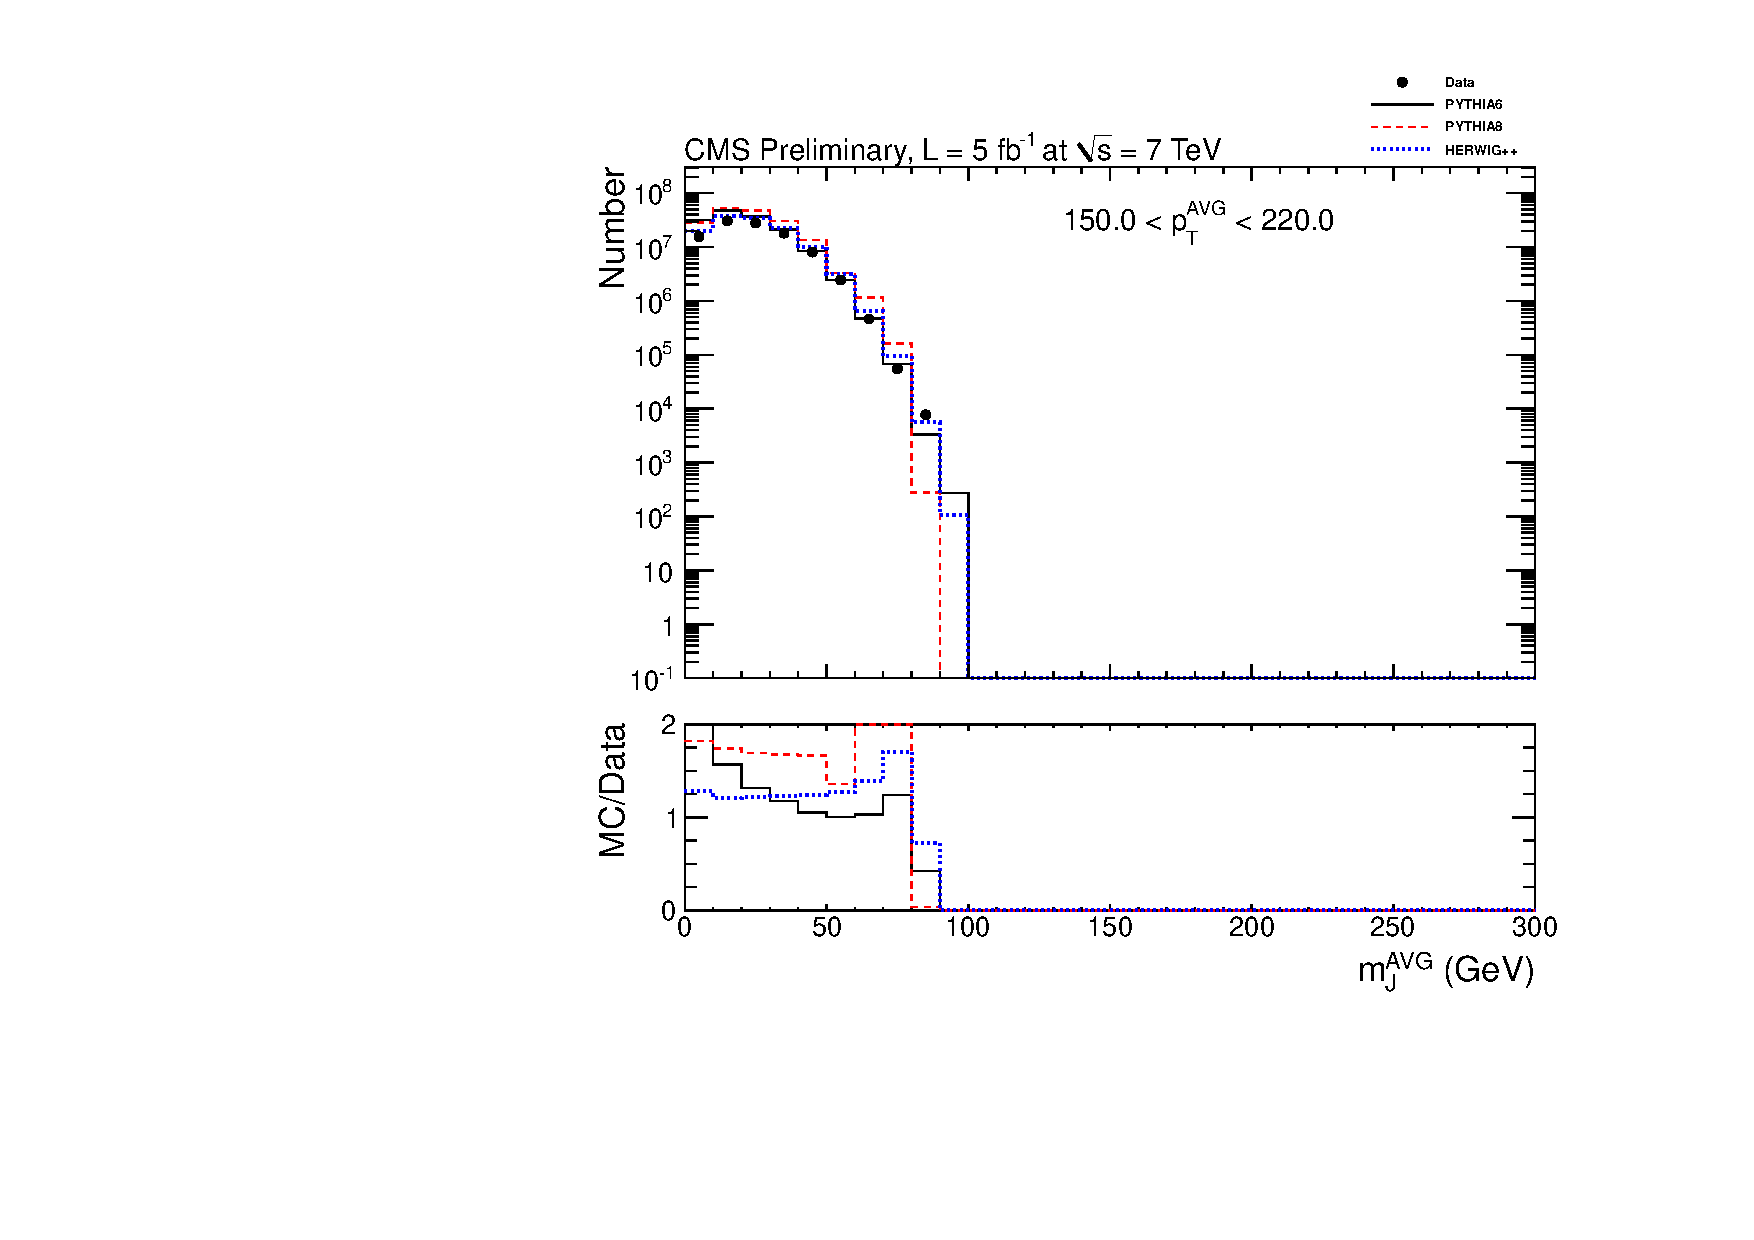
\includegraphics[width=0.95\textwidth]{figs/histAK7MjetVsPtAvg_rawDataMCComparisons_pt_3_Pruned}
\caption{Detector-level distributions of the jet mass for AK7 Pruned jets,
for $150.0 < \pt^{AVG} < 220.0$ \GeVc. The data are shown in black points.
The simulated distribution from \PYTHIA is shown in solid black, 
the from \PYTHIAEIGHT in dashed red, and from \HERWIG in dotted blue. 
The bottom frame shows the ratio of the simulated distribution
to the distribution from data. 
\label{figs:histAK7MjetVsPtAvg_rawDataMCComparisons_pt_3_Pruned}}
\end{figure}



\begin{figure}[htbp]
\centering
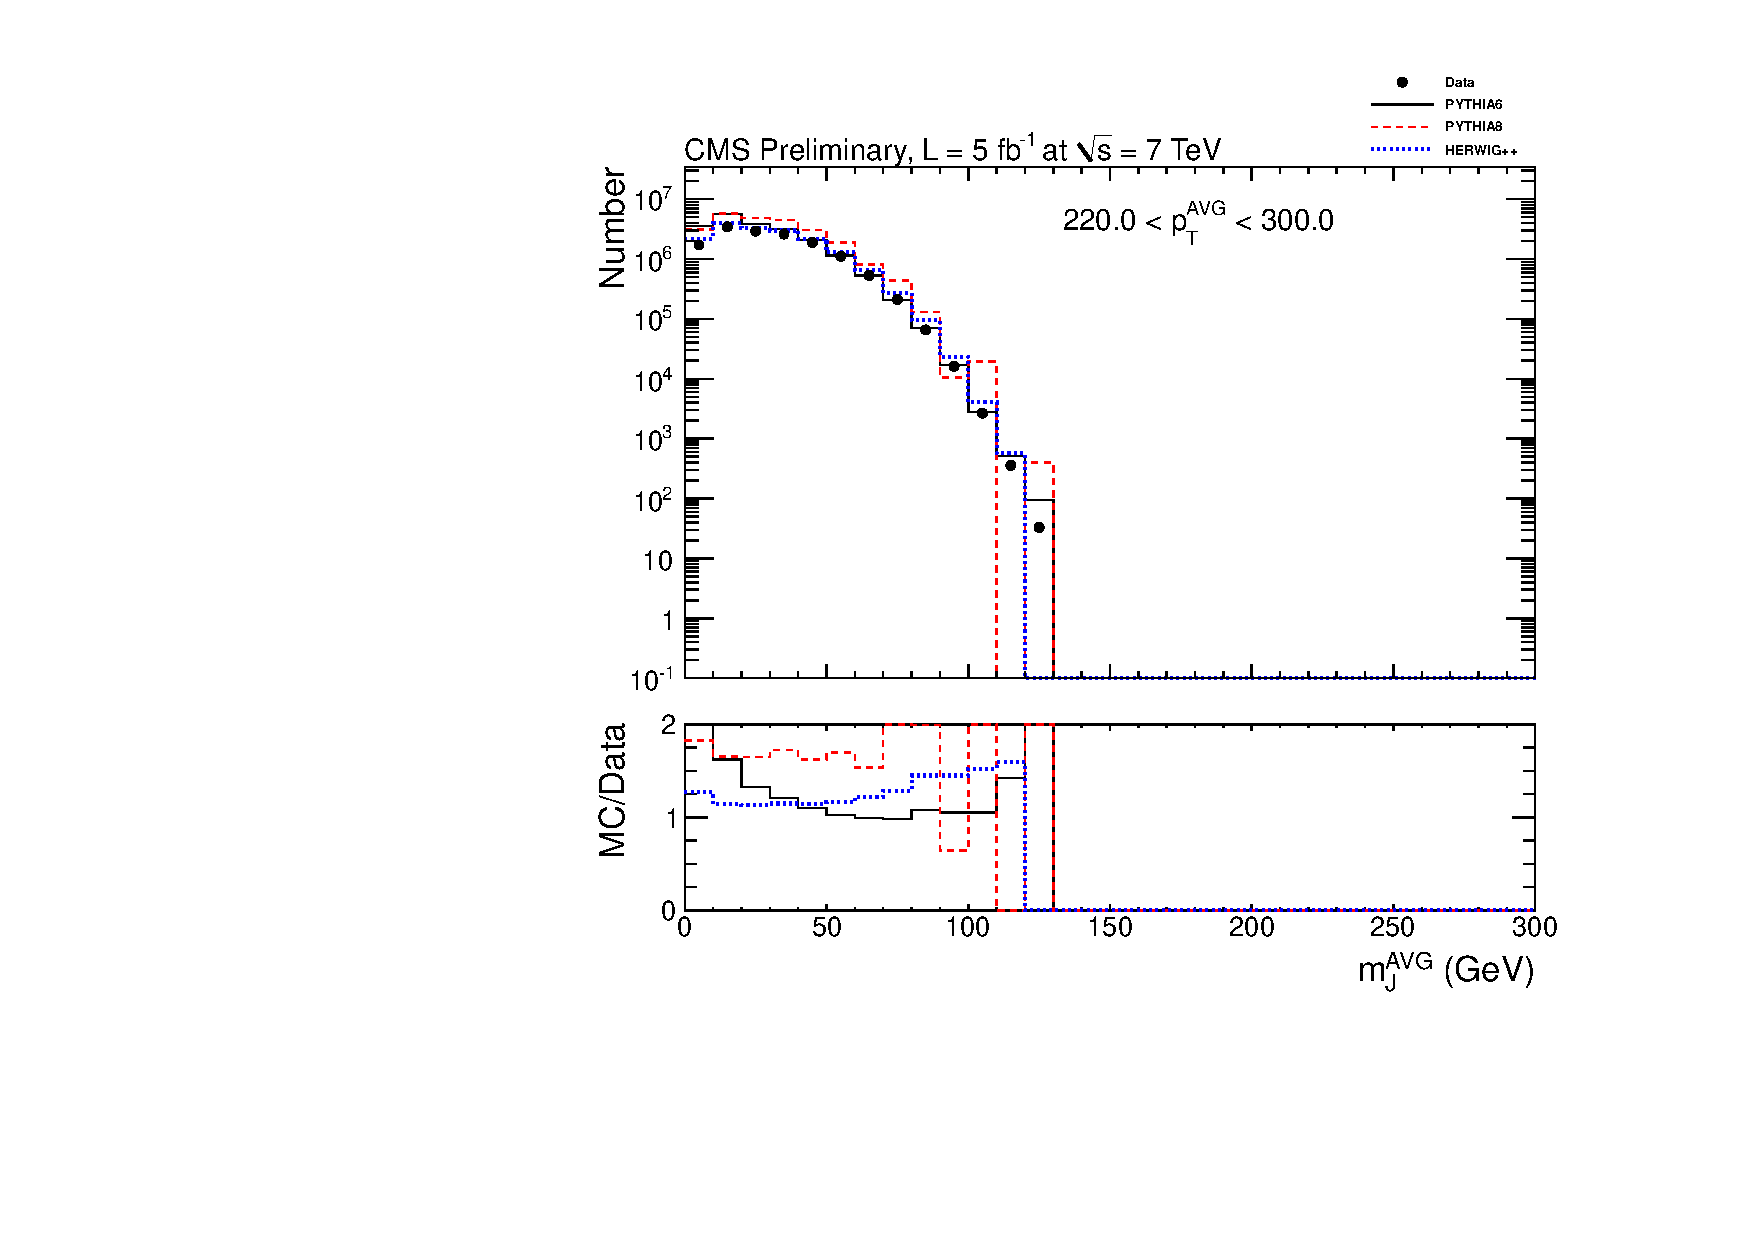
\includegraphics[width=0.95\textwidth]{figs/histAK7MjetVsPtAvg_rawDataMCComparisons_pt_4_Pruned}
\caption{Detector-level distributions of the jet mass for AK7 Pruned jets,
for $220.0 < \pt^{AVG} < 300.0$ \GeVc. The data are shown in black points.
The simulated distribution from \PYTHIA is shown in solid black, 
the from \PYTHIAEIGHT in dashed red, and from \HERWIG in dotted blue. 
The bottom frame shows the ratio of the simulated distribution
to the distribution from data. 
\label{figs:histAK7MjetVsPtAvg_rawDataMCComparisons_pt_4_Pruned}}
\end{figure}



\begin{figure}[htbp]
\centering
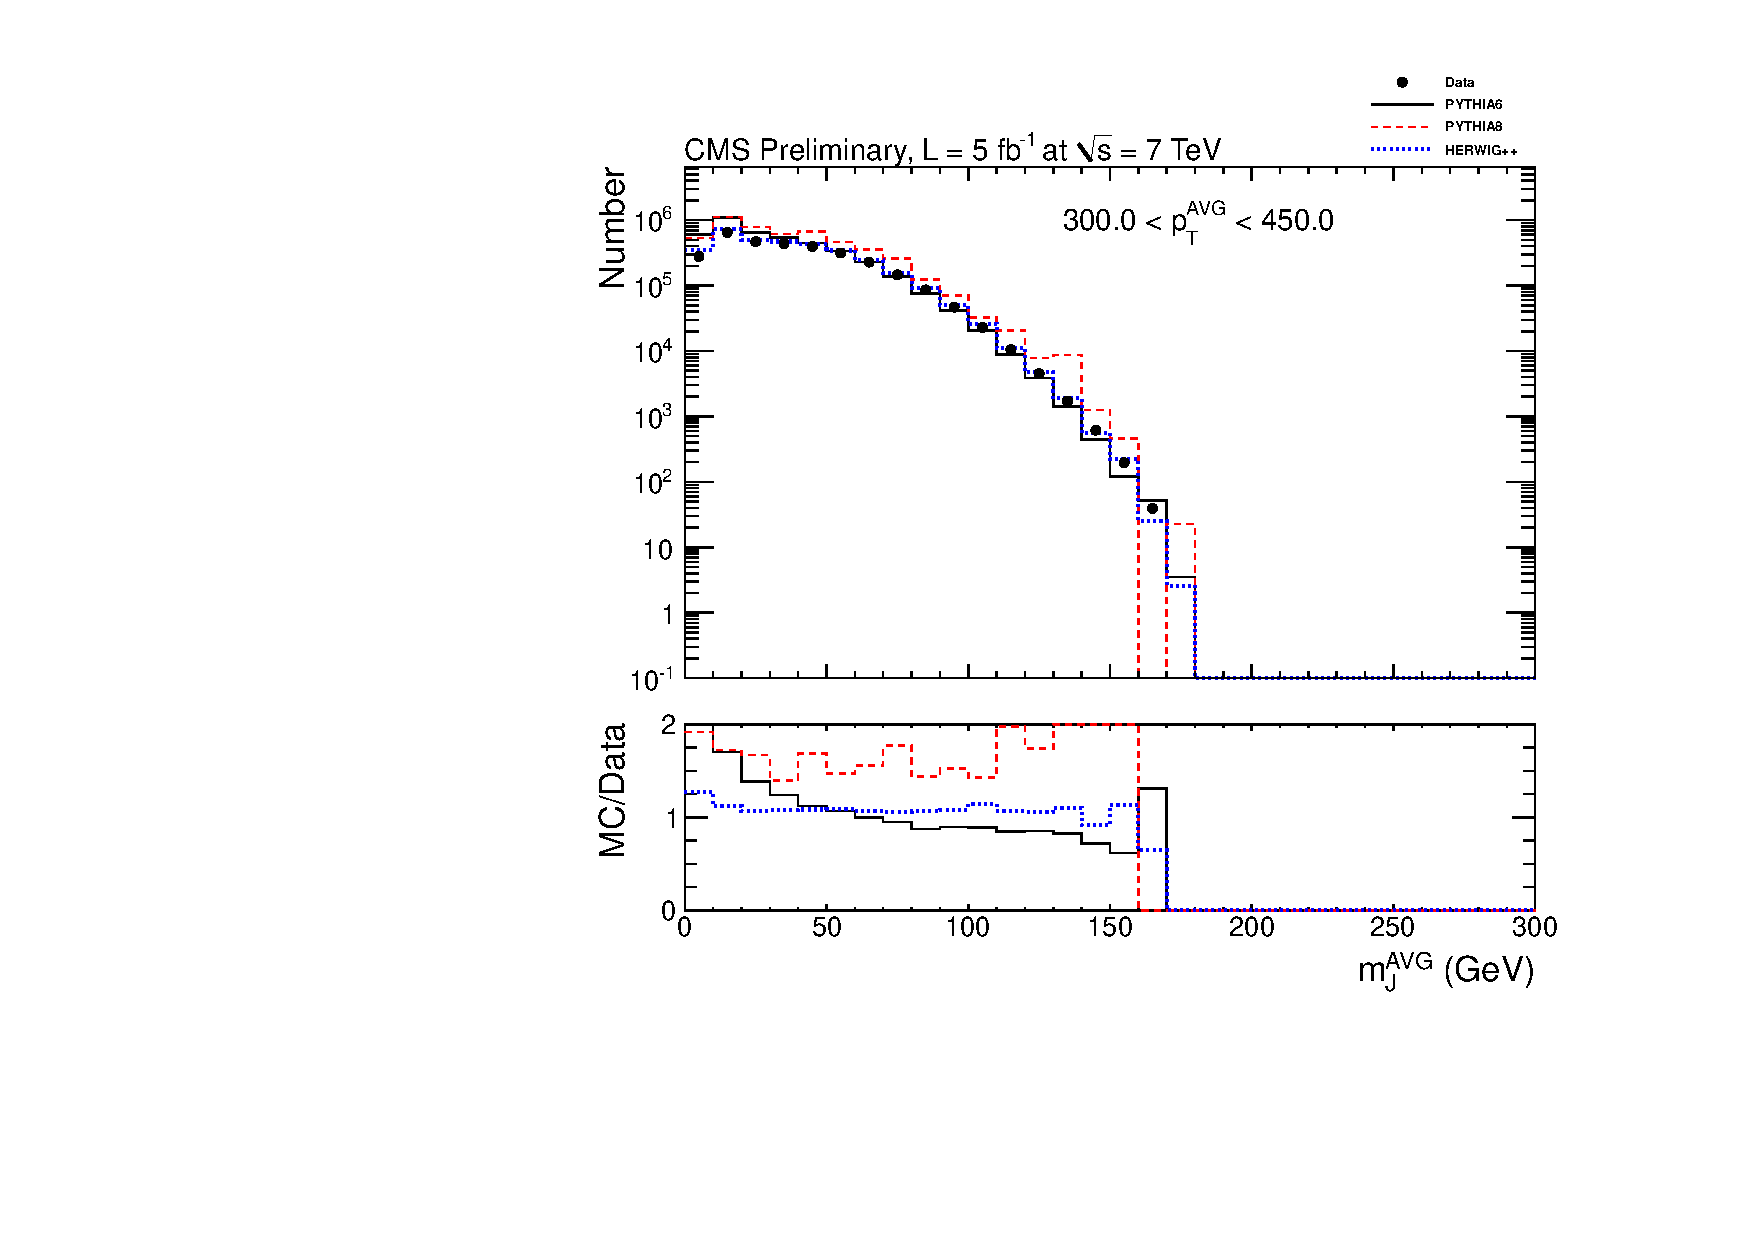
\includegraphics[width=0.95\textwidth]{figs/histAK7MjetVsPtAvg_rawDataMCComparisons_pt_5_Pruned}
\caption{Detector-level distributions of the jet mass for AK7 Pruned jets,
for $300.0 < \pt^{AVG} < 450.0$ \GeVc. The data are shown in black points.
The simulated distribution from \PYTHIA is shown in solid black, 
the from \PYTHIAEIGHT in dashed red, and from \HERWIG in dotted blue. 
The bottom frame shows the ratio of the simulated distribution
to the distribution from data. 
\label{figs:histAK7MjetVsPtAvg_rawDataMCComparisons_pt_5_Pruned}}
\end{figure}



\begin{figure}[htbp]
\centering
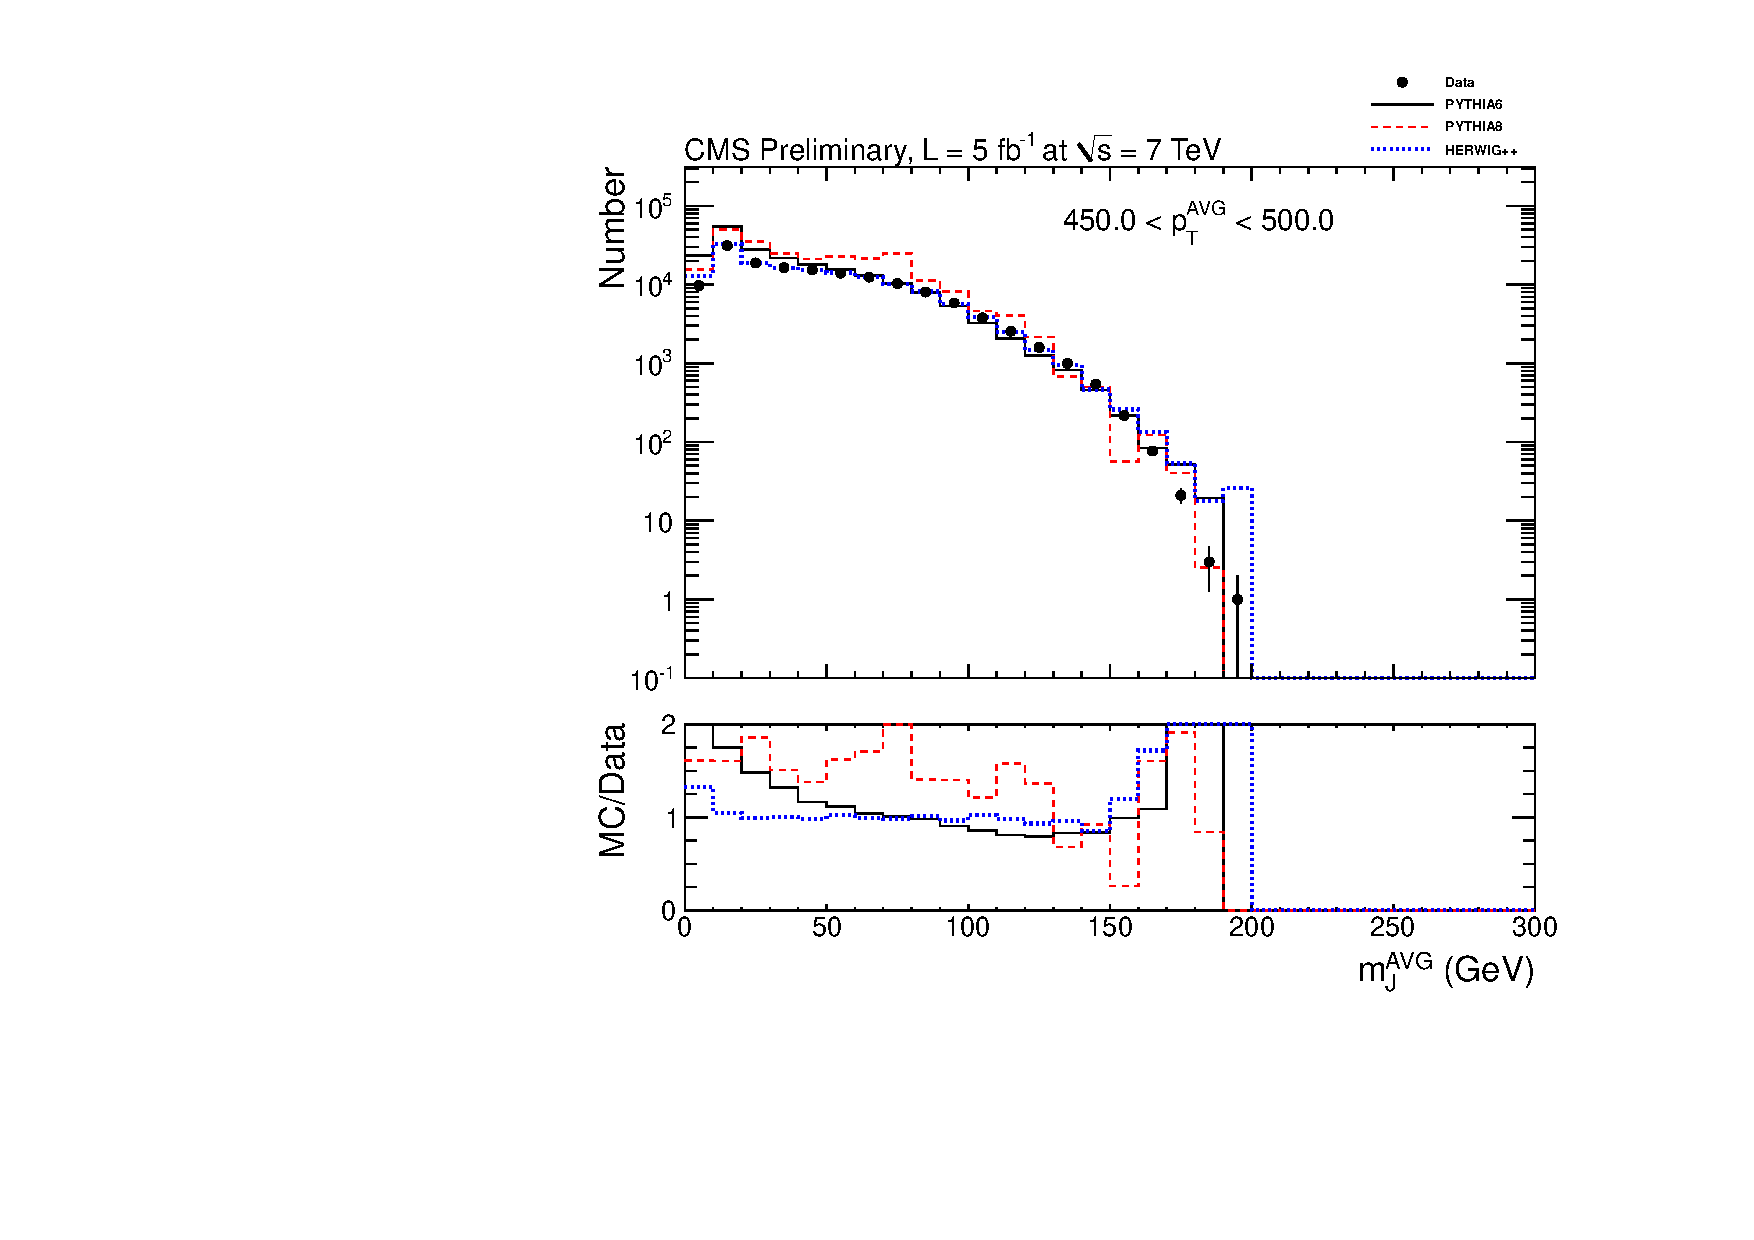
\includegraphics[width=0.95\textwidth]{figs/histAK7MjetVsPtAvg_rawDataMCComparisons_pt_6_Pruned}
\caption{Detector-level distributions of the jet mass for AK7 Pruned jets,
for $450.0 < \pt^{AVG} < 500.0$ \GeVc. The data are shown in black points.
The simulated distribution from \PYTHIA is shown in solid black, 
the from \PYTHIAEIGHT in dashed red, and from \HERWIG in dotted blue. 
The bottom frame shows the ratio of the simulated distribution
to the distribution from data. 
\label{figs:histAK7MjetVsPtAvg_rawDataMCComparisons_pt_6_Pruned}}
\end{figure}



\begin{figure}[htbp]
\centering
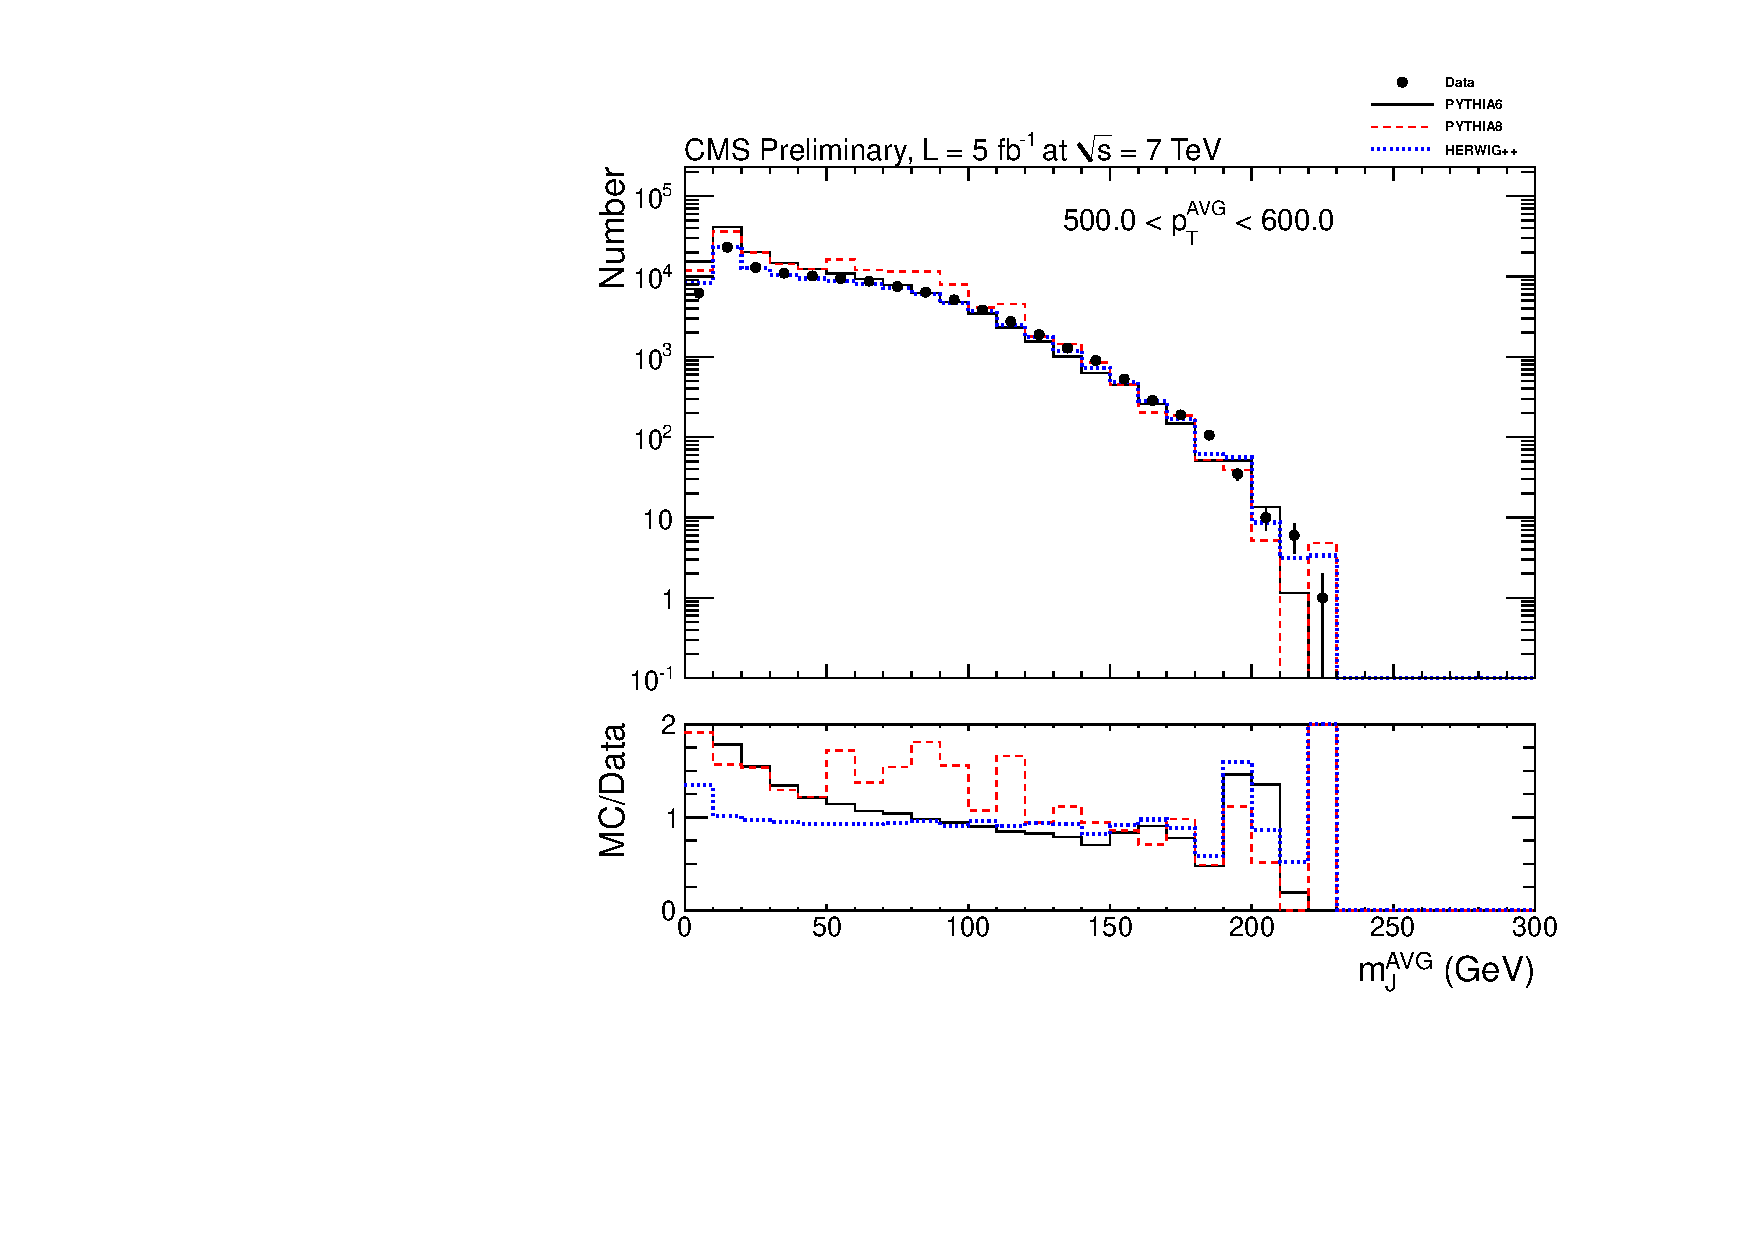
\includegraphics[width=0.95\textwidth]{figs/histAK7MjetVsPtAvg_rawDataMCComparisons_pt_7_Pruned}
\caption{Detector-level distributions of the jet mass for AK7 Pruned jets,
for $500.0 < \pt^{AVG} < 600.0$ \GeVc. The data are shown in black points.
The simulated distribution from \PYTHIA is shown in solid black, 
the from \PYTHIAEIGHT in dashed red, and from \HERWIG in dotted blue. 
The bottom frame shows the ratio of the simulated distribution
to the distribution from data. 
\label{figs:histAK7MjetVsPtAvg_rawDataMCComparisons_pt_7_Pruned}}
\end{figure}



\begin{figure}[htbp]
\centering
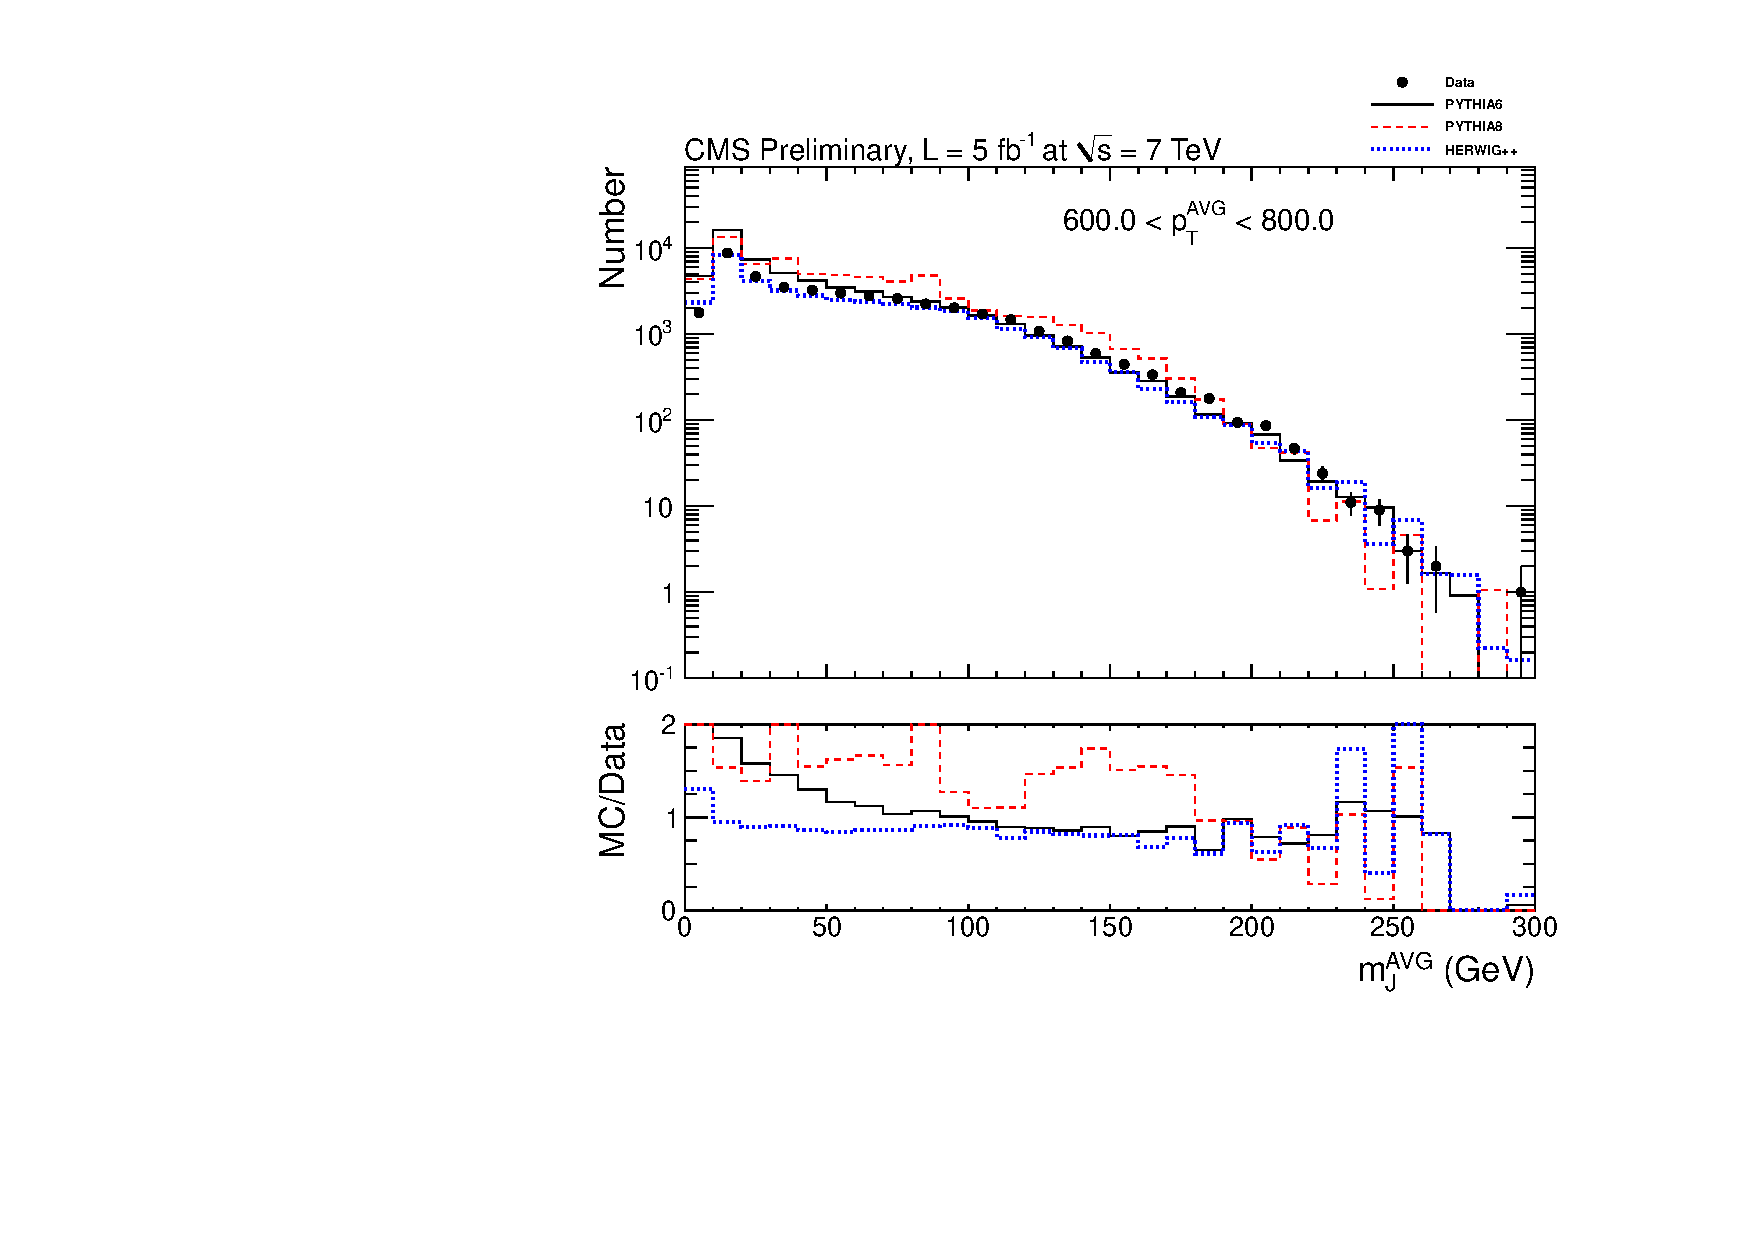
\includegraphics[width=0.95\textwidth]{figs/histAK7MjetVsPtAvg_rawDataMCComparisons_pt_8_Pruned}
\caption{Detector-level distributions of the jet mass for AK7 Pruned jets,
for $600.0 < \pt^{AVG} < 800.0$ \GeVc. The data are shown in black points.
The simulated distribution from \PYTHIA is shown in solid black, 
the from \PYTHIAEIGHT in dashed red, and from \HERWIG in dotted blue. 
The bottom frame shows the ratio of the simulated distribution
to the distribution from data. 
\label{figs:histAK7MjetVsPtAvg_rawDataMCComparisons_pt_8_Pruned}}
\end{figure}



\begin{figure}[htbp]
\centering
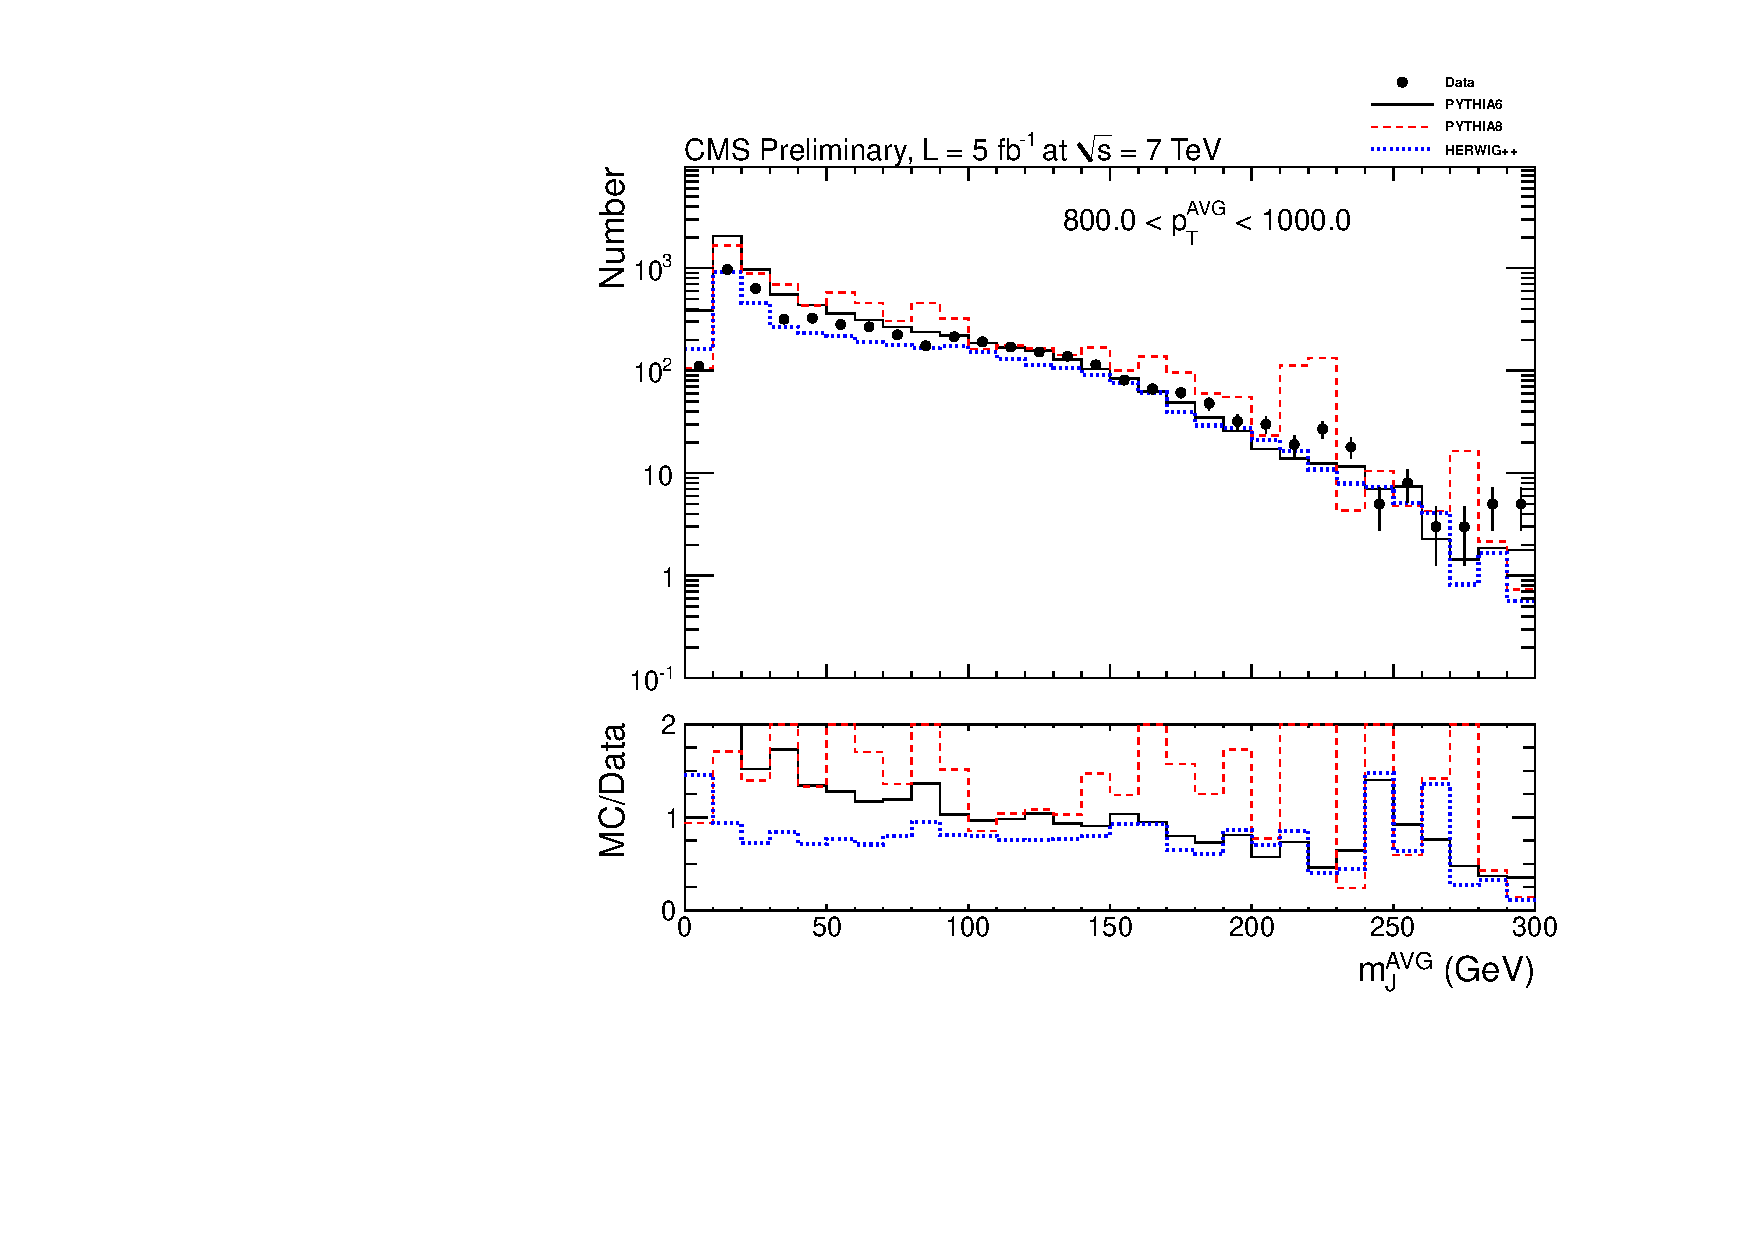
\includegraphics[width=0.95\textwidth]{figs/histAK7MjetVsPtAvg_rawDataMCComparisons_pt_9_Pruned}
\caption{Detector-level distributions of the jet mass for AK7 Pruned jets,
for $800.0 < \pt^{AVG} < 1000.0$ \GeVc. The data are shown in black points.
The simulated distribution from \PYTHIA is shown in solid black, 
the from \PYTHIAEIGHT in dashed red, and from \HERWIG in dotted blue. 
The bottom frame shows the ratio of the simulated distribution
to the distribution from data. 
\label{figs:histAK7MjetVsPtAvg_rawDataMCComparisons_pt_9_Pruned}}
\end{figure}



\begin{figure}[htbp]
\centering
\includegraphics[width=0.95\textwidth]{figs/histAK7MjetVsPtAvg_rawDataMCComparisons_pt_10_Pruned}
\caption{Detector-level distributions of the jet mass for AK7 Pruned jets,
for $1000.0 < \pt^{AVG} < 1500.0$ \GeVc. The data are shown in black points.
The simulated distribution from \PYTHIA is shown in solid black, 
the from \PYTHIAEIGHT in dashed red, and from \HERWIG in dotted blue. 
The bottom frame shows the ratio of the simulated distribution
to the distribution from data. 
\label{figs:histAK7MjetVsPtAvg_rawDataMCComparisons_pt_10_Pruned}}
\end{figure}


\clearpage



\begin{figure}[htbp]
\centering
\includegraphics[width=0.95\textwidth]{figs/unfoldedMeasurementDijets_all_}
\caption{Unfolded distributions for the mean mass of the two leading jets in dijet events for reconstructed AK7 jets,
separated according to intervals in $\pt^{AVG}$ (the mean $\pt$ of the two jets).
The data are shown by the symbols indicating different bins in the mean $\pt$ of the two jets. 
The statistical uncertainty is shown in light shading, and the
total uncertainty in dark shading. 
Predictions
from \HERWIG are given by the dotted lines. 
To enhance visibility, the distributions for larger values of $\pt^{AVG}$ 
are scaled up by the factors given in the legend.
\label{figs:unfoldedMeasurementDijets_all}}
\end{figure}

\begin{figure}[htbp]
\centering
\includegraphics[width=0.95\textwidth]{figs/unfoldedMeasurementDijets_all__Filtered}
\caption{Unfolded distributions for the mean mass of the two leading jets in dijet events for reconstructed filtered AK7 jets,
separated according to intervals in $\pt^{AVG}$ (the mean $\pt$ of the two jets).
The data are shown by the symbols indicating different bins in the mean $\pt$ of the two jets. 
The statistical uncertainty is shown in light shading, and the
total uncertainty in dark shading. 
Predictions
from \HERWIG are given by the dotted lines. 
To enhance visibility, the distributions for larger values of $\pt^{AVG}$ 
are scaled up by the factors given in the legend. 
\label{figs:unfoldedMeasurementDijets_all_Filtered}}
\end{figure}

\begin{figure}[htbp]
\centering
\includegraphics[width=0.95\textwidth]{figs/unfoldedMeasurementDijets_all__Trimmed}
\caption{Unfolded distributions for the mean mass of the two leading jets in dijet events for reconstructed trimmed AK7 jets,
separated according to intervals in $\pt^{AVG}$ (the mean $\pt$ of the two jets).
The data are shown by the symbols indicating different bins in the mean $\pt$ of the two jets. 
The statistical uncertainty is shown in light shading, and the
total uncertainty in dark shading. 
Predictions
from \HERWIG are given by the dotted lines. 
To enhance visibility, the distributions for larger values of $\pt^{AVG}$ 
are scaled up by the factors given in the legend. 
\label{figs:unfoldedMeasurementDijets_all_Trimmed}}
\end{figure}

\begin{figure}[htbp]
\centering
\includegraphics[width=0.95\textwidth]{figs/unfoldedMeasurementDijets_all__Pruned}
\caption{Unfolded distributions for the mean mass of the two leading jets in dijet events for reconstructed pruned AK7 jets,
separated according to intervals in $\pt^{AVG}$ (the mean $\pt$ of the two jets).
The data are shown by the symbols indicating different bins in the mean $\pt$ of the two jets. 
The statistical uncertainty is shown in light shading, and the
total uncertainty in dark shading. 
Predictions
from \HERWIG are given by the dotted lines. 
To enhance visibility, the distributions for larger values of $\pt^{AVG}$ 
are scaled up by the factors given in the legend. 
\label{figs:unfoldedMeasurementDijets_all_Pruned}}
\end{figure}

\begin{figure}[htbp]
\centering
\includegraphics[width=0.95\textwidth]{figs/unfoldedMeasurementDijets_allfrac_}
\caption{Ratio of MC simulation to unfolded distributions of the jet mass for AK7 jets for the seven bins in $\pt^{AVG}$.
The statistical uncertainty is shown in light shading, and the
total uncertainty is shown in dark shading.
The comparison for \PYTHIA is shown in solid lines, for \PYTHIAEIGHT in dashed lines, and for \HERWIG in dotted lines.
\label{figs:unfoldedMeasurementDijets_allfrac}}
\end{figure}


\begin{figure}[htbp]
\centering
\includegraphics[width=0.95\textwidth]{figs/unfoldedMeasurementDijets_allfrac__Filtered}
\caption{Ratio of MC simulation to unfolded distributions of the jet mass for filtered AK7 jets for the seven bins in $\pt^{AVG}$.
The statistical uncertainty is shown in light shading, and the
total uncertainty is shown in dark shading.
The comparison for \PYTHIA is shown in solid lines, for \PYTHIAEIGHT in dashed lines, and for \HERWIG in dotted lines.
\label{figs:unfoldedMeasurementDijets_allfrac_Filtered}}
\end{figure}


\begin{figure}[htbp]
\centering
\includegraphics[width=0.95\textwidth]{figs/unfoldedMeasurementDijets_allfrac__Trimmed}
\caption{Ratio of MC simulation to unfolded distributions of the jet mass for trimmed AK7 jets for the seven bins in $\pt^{AVG}$.
The statistical uncertainty is shown in light shading, and the
total uncertainty is shown in dark shading.
The comparison for \PYTHIA is shown in solid lines, for \PYTHIAEIGHT in dashed lines, and for \HERWIG in dotted lines.
\label{figs:unfoldedMeasurementDijets_allfrac_Trimmed}}
\end{figure}

\begin{figure}[htbp]
\centering
\includegraphics[width=0.95\textwidth]{figs/unfoldedMeasurementDijets_allfrac__Pruned}
\caption{Ratio of MC simulation to unfolded distributions of the jet mass for pruned AK7 jets for the seven bins in $\pt^{AVG}$.
The statistical uncertainty is shown in light shading, and the
total uncertainty is shown in dark shading.
The comparison for \PYTHIA is shown in solid lines, for \PYTHIAEIGHT in dashed lines, and for \HERWIG in dotted lines.
\label{figs:unfoldedMeasurementDijets_allfrac_Pruned}}
\end{figure}









%\ifnpas

\begin{figure}[htbp]
\centering
\includegraphics[width=0.95\textwidth]{figs/unfoldedMeasurementDijets_1_allsys}
\caption{Unfolded distributions of the jet mass for AK7 jets,
for $50.0 < \pt^{AVG} < 125.0$ \GeVc. The data are shown in black
points. 
The statistical uncertainty is shown in light yellow, the uncertainties due to the jet-energy resolution, jet-energy scale, and jet-angular resolution are shown in shades of brown, the uncertainty due to pile-up is shown in green, and the uncertainty due to the parton shower are shown in dark yellow.
The simulated distribution from \PYTHIA is shown in solid black, 
the from \PYTHIAEIGHT in dashed red, and from \HERWIG in dotted blue. 
The bottom frame shows the ratio of the true distribution from
the simulation divided by the unfolded distribution, along with
the uncertainties in the unfolded distribution. 
\label{figs:unfoldedMeasurementDijets_1_allsys}}
\end{figure}



\begin{figure}[htbp]
\centering
\includegraphics[width=0.95\textwidth]{figs/unfoldedMeasurementDijets_2_allsys}
\caption{Unfolded distributions of the jet mass for AK7 jets,
for $125.0 < \pt^{AVG} < 150.0$ \GeVc. The data are shown in black
points. 
The statistical uncertainty is shown in light yellow, the uncertainties due to the jet-energy resolution, jet-energy scale, and jet-angular resolution are shown in shades of brown, the uncertainty due to pile-up is shown in green, and the uncertainty due to the parton shower are shown in dark yellow.
The simulated distribution from \PYTHIA is shown in solid black, 
the from \PYTHIAEIGHT in dashed red, and from \HERWIG in dotted blue. 
The bottom frame shows the ratio of the true distribution from
the simulation divided by the unfolded distribution, along with
the uncertainties in the unfolded distribution. 
\label{figs:unfoldedMeasurementDijets_2_allsys}}
\end{figure}



\begin{figure}[htbp]
\centering
\includegraphics[width=0.95\textwidth]{figs/unfoldedMeasurementDijets_3_allsys}
\caption{Unfolded distributions of the jet mass for AK7 jets,
for $150.0 < \pt^{AVG} < 220.0$ \GeVc. The data are shown in black
points. 
The statistical uncertainty is shown in light yellow, the uncertainties due to the jet-energy resolution, jet-energy scale, and jet-angular resolution are shown in shades of brown, the uncertainty due to pile-up is shown in green, and the uncertainty due to the parton shower are shown in dark yellow.
The simulated distribution from \PYTHIA is shown in solid black, 
the from \PYTHIAEIGHT in dashed red, and from \HERWIG in dotted blue. 
The bottom frame shows the ratio of the true distribution from
the simulation divided by the unfolded distribution, along with
the uncertainties in the unfolded distribution. 
\label{figs:unfoldedMeasurementDijets_3_allsys}}
\end{figure}



\begin{figure}[htbp]
\centering
\includegraphics[width=0.95\textwidth]{figs/unfoldedMeasurementDijets_4_allsys}
\caption{Unfolded distributions of the jet mass for AK7 jets,
for $220.0 < \pt^{AVG} < 300.0$ \GeVc. The data are shown in black
points. 
The statistical uncertainty is shown in light yellow, the uncertainties due to the jet-energy resolution, jet-energy scale, and jet-angular resolution are shown in shades of brown, the uncertainty due to pile-up is shown in green, and the uncertainty due to the parton shower are shown in dark yellow.
The simulated distribution from \PYTHIA is shown in solid black, 
the from \PYTHIAEIGHT in dashed red, and from \HERWIG in dotted blue. 
The bottom frame shows the ratio of the true distribution from
the simulation divided by the unfolded distribution, along with
the uncertainties in the unfolded distribution. 
\label{figs:unfoldedMeasurementDijets_4_allsys}}
\end{figure}



\begin{figure}[htbp]
\centering
\includegraphics[width=0.95\textwidth]{figs/unfoldedMeasurementDijets_5_allsys}
\caption{Unfolded distributions of the jet mass for AK7 jets,
for $300.0 < \pt^{AVG} < 450.0$ \GeVc. The data are shown in black
points. 
The statistical uncertainty is shown in light yellow, the uncertainties due to the jet-energy resolution, jet-energy scale, and jet-angular resolution are shown in shades of brown, the uncertainty due to pile-up is shown in green, and the uncertainty due to the parton shower are shown in dark yellow.
The simulated distribution from \PYTHIA is shown in solid black, 
the from \PYTHIAEIGHT in dashed red, and from \HERWIG in dotted blue. 
The bottom frame shows the ratio of the true distribution from
the simulation divided by the unfolded distribution, along with
the uncertainties in the unfolded distribution. 
\label{figs:unfoldedMeasurementDijets_5_allsys}}
\end{figure}



\begin{figure}[htbp]
\centering
\includegraphics[width=0.95\textwidth]{figs/unfoldedMeasurementDijets_6_allsys}
\caption{Unfolded distributions of the jet mass for AK7 jets,
for $450.0 < \pt^{AVG} < 500.0$ \GeVc. The data are shown in black
points. 
The statistical uncertainty is shown in light yellow, the uncertainties due to the jet-energy resolution, jet-energy scale, and jet-angular resolution are shown in shades of brown, the uncertainty due to pile-up is shown in green, and the uncertainty due to the parton shower are shown in dark yellow.
The simulated distribution from \PYTHIA is shown in solid black, 
the from \PYTHIAEIGHT in dashed red, and from \HERWIG in dotted blue. 
The bottom frame shows the ratio of the true distribution from
the simulation divided by the unfolded distribution, along with
the uncertainties in the unfolded distribution. 
\label{figs:unfoldedMeasurementDijets_6_allsys}}
\end{figure}



\begin{figure}[htbp]
\centering
\includegraphics[width=0.95\textwidth]{figs/unfoldedMeasurementDijets_7_allsys}
\caption{Unfolded distributions of the jet mass for AK7 jets,
for $500.0 < \pt^{AVG} < 600.0$ \GeVc. The data are shown in black
points. 
The statistical uncertainty is shown in light yellow, the uncertainties due to the jet-energy resolution, jet-energy scale, and jet-angular resolution are shown in shades of brown, the uncertainty due to pile-up is shown in green, and the uncertainty due to the parton shower are shown in dark yellow.
The simulated distribution from \PYTHIA is shown in solid black, 
the from \PYTHIAEIGHT in dashed red, and from \HERWIG in dotted blue. 
The bottom frame shows the ratio of the true distribution from
the simulation divided by the unfolded distribution, along with
the uncertainties in the unfolded distribution. 
\label{figs:unfoldedMeasurementDijets_7_allsys}}
\end{figure}



\begin{figure}[htbp]
\centering
\includegraphics[width=0.95\textwidth]{figs/unfoldedMeasurementDijets_8_allsys}
\caption{Unfolded distributions of the jet mass for AK7 jets,
for $600.0 < \pt^{AVG} < 800.0$ \GeVc. The data are shown in black
points. 
The statistical uncertainty is shown in light yellow, the uncertainties due to the jet-energy resolution, jet-energy scale, and jet-angular resolution are shown in shades of brown, the uncertainty due to pile-up is shown in green, and the uncertainty due to the parton shower are shown in dark yellow.
The simulated distribution from \PYTHIA is shown in solid black, 
the from \PYTHIAEIGHT in dashed red, and from \HERWIG in dotted blue. 
The bottom frame shows the ratio of the true distribution from
the simulation divided by the unfolded distribution, along with
the uncertainties in the unfolded distribution. 
\label{figs:unfoldedMeasurementDijets_8_allsys}}
\end{figure}



\begin{figure}[htbp]
\centering
\includegraphics[width=0.95\textwidth]{figs/unfoldedMeasurementDijets_9_allsys}
\caption{Unfolded distributions of the jet mass for AK7 jets,
for $800.0 < \pt^{AVG} < 1000.0$ \GeVc. The data are shown in black
points. 
The statistical uncertainty is shown in light yellow, the uncertainties due to the jet-energy resolution, jet-energy scale, and jet-angular resolution are shown in shades of brown, the uncertainty due to pile-up is shown in green, and the uncertainty due to the parton shower are shown in dark yellow.
The simulated distribution from \PYTHIA is shown in solid black, 
the from \PYTHIAEIGHT in dashed red, and from \HERWIG in dotted blue. 
The bottom frame shows the ratio of the true distribution from
the simulation divided by the unfolded distribution, along with
the uncertainties in the unfolded distribution. 
\label{figs:unfoldedMeasurementDijets_9_allsys}}
\end{figure}



\begin{figure}[htbp]
\centering
\includegraphics[width=0.95\textwidth]{figs/unfoldedMeasurementDijets_10_allsys}
\caption{Unfolded distributions of the jet mass for AK7 jets,
for $1000.0 < \pt^{AVG} < 1500.0$ \GeVc. The data are shown in black
points. 
The statistical uncertainty is shown in light yellow, the uncertainties due to the jet-energy resolution, jet-energy scale, and jet-angular resolution are shown in shades of brown, the uncertainty due to pile-up is shown in green, and the uncertainty due to the parton shower are shown in dark yellow.
The simulated distribution from \PYTHIA is shown in solid black, 
the from \PYTHIAEIGHT in dashed red, and from \HERWIG in dotted blue. 
The bottom frame shows the ratio of the true distribution from
the simulation divided by the unfolded distribution, along with
the uncertainties in the unfolded distribution. 
\label{figs:unfoldedMeasurementDijets_10_allsys}}
\end{figure}

\clearpage

\begin{figure}[htbp]
\centering
\includegraphics[width=0.95\textwidth]{figs/unfoldedMeasurementDijets_1_Filtered_allsys}
\caption{Unfolded distributions of the jet mass for AK7 Filtered jets,
for $50.0 < \pt^{AVG} < 125.0$ \GeVc. The data are shown in black
points. 
The statistical uncertainty is shown in light yellow, the uncertainties due to the jet-energy resolution, jet-energy scale, and jet-angular resolution are shown in shades of brown, the uncertainty due to pile-up is shown in green, and the uncertainty due to the parton shower are shown in dark yellow.
The simulated distribution from \PYTHIA is shown in solid black, 
the from \PYTHIAEIGHT in dashed red, and from \HERWIG in dotted blue. 
The bottom frame shows the ratio of the true distribution from
the simulation divided by the unfolded distribution, along with
the uncertainties in the unfolded distribution. 
\label{figs:unfoldedMeasurementDijets_1_Filtered_allsys}}
\end{figure}



\begin{figure}[htbp]
\centering
\includegraphics[width=0.95\textwidth]{figs/unfoldedMeasurementDijets_2_Filtered_allsys}
\caption{Unfolded distributions of the jet mass for AK7 Filtered jets,
for $125.0 < \pt^{AVG} < 150.0$ \GeVc. The data are shown in black
points. 
The statistical uncertainty is shown in light yellow, the uncertainties due to the jet-energy resolution, jet-energy scale, and jet-angular resolution are shown in shades of brown, the uncertainty due to pile-up is shown in green, and the uncertainty due to the parton shower are shown in dark yellow.
The simulated distribution from \PYTHIA is shown in solid black, 
the from \PYTHIAEIGHT in dashed red, and from \HERWIG in dotted blue. 
The bottom frame shows the ratio of the true distribution from
the simulation divided by the unfolded distribution, along with
the uncertainties in the unfolded distribution. 
\label{figs:unfoldedMeasurementDijets_2_Filtered_allsys}}
\end{figure}



\begin{figure}[htbp]
\centering
\includegraphics[width=0.95\textwidth]{figs/unfoldedMeasurementDijets_3_Filtered_allsys}
\caption{Unfolded distributions of the jet mass for AK7 Filtered jets,
for $150.0 < \pt^{AVG} < 220.0$ \GeVc. The data are shown in black
points. 
The statistical uncertainty is shown in light yellow, the uncertainties due to the jet-energy resolution, jet-energy scale, and jet-angular resolution are shown in shades of brown, the uncertainty due to pile-up is shown in green, and the uncertainty due to the parton shower are shown in dark yellow.
The simulated distribution from \PYTHIA is shown in solid black, 
the from \PYTHIAEIGHT in dashed red, and from \HERWIG in dotted blue. 
The bottom frame shows the ratio of the true distribution from
the simulation divided by the unfolded distribution, along with
the uncertainties in the unfolded distribution. 
\label{figs:unfoldedMeasurementDijets_3_Filtered_allsys}}
\end{figure}



\begin{figure}[htbp]
\centering
\includegraphics[width=0.95\textwidth]{figs/unfoldedMeasurementDijets_4_Filtered_allsys}
\caption{Unfolded distributions of the jet mass for AK7 Filtered jets,
for $220.0 < \pt^{AVG} < 300.0$ \GeVc. The data are shown in black
points. 
The statistical uncertainty is shown in light yellow, the uncertainties due to the jet-energy resolution, jet-energy scale, and jet-angular resolution are shown in shades of brown, the uncertainty due to pile-up is shown in green, and the uncertainty due to the parton shower are shown in dark yellow.
The simulated distribution from \PYTHIA is shown in solid black, 
the from \PYTHIAEIGHT in dashed red, and from \HERWIG in dotted blue. 
The bottom frame shows the ratio of the true distribution from
the simulation divided by the unfolded distribution, along with
the uncertainties in the unfolded distribution. 
\label{figs:unfoldedMeasurementDijets_4_Filtered_allsys}}
\end{figure}



\begin{figure}[htbp]
\centering
\includegraphics[width=0.95\textwidth]{figs/unfoldedMeasurementDijets_5_Filtered_allsys}
\caption{Unfolded distributions of the jet mass for AK7 Filtered jets,
for $300.0 < \pt^{AVG} < 450.0$ \GeVc. The data are shown in black
points. 
The statistical uncertainty is shown in light yellow, the uncertainties due to the jet-energy resolution, jet-energy scale, and jet-angular resolution are shown in shades of brown, the uncertainty due to pile-up is shown in green, and the uncertainty due to the parton shower are shown in dark yellow.
The simulated distribution from \PYTHIA is shown in solid black, 
the from \PYTHIAEIGHT in dashed red, and from \HERWIG in dotted blue. 
The bottom frame shows the ratio of the true distribution from
the simulation divided by the unfolded distribution, along with
the uncertainties in the unfolded distribution. 
\label{figs:unfoldedMeasurementDijets_5_Filtered_allsys}}
\end{figure}



\begin{figure}[htbp]
\centering
\includegraphics[width=0.95\textwidth]{figs/unfoldedMeasurementDijets_6_Filtered_allsys}
\caption{Unfolded distributions of the jet mass for AK7 Filtered jets,
for $450.0 < \pt^{AVG} < 500.0$ \GeVc. The data are shown in black
points. 
The statistical uncertainty is shown in light yellow, the uncertainties due to the jet-energy resolution, jet-energy scale, and jet-angular resolution are shown in shades of brown, the uncertainty due to pile-up is shown in green, and the uncertainty due to the parton shower are shown in dark yellow.
The simulated distribution from \PYTHIA is shown in solid black, 
the from \PYTHIAEIGHT in dashed red, and from \HERWIG in dotted blue. 
The bottom frame shows the ratio of the true distribution from
the simulation divided by the unfolded distribution, along with
the uncertainties in the unfolded distribution. 
\label{figs:unfoldedMeasurementDijets_6_Filtered_allsys}}
\end{figure}



\begin{figure}[htbp]
\centering
\includegraphics[width=0.95\textwidth]{figs/unfoldedMeasurementDijets_7_Filtered_allsys}
\caption{Unfolded distributions of the jet mass for AK7 Filtered jets,
for $500.0 < \pt^{AVG} < 600.0$ \GeVc. The data are shown in black
points. 
The statistical uncertainty is shown in light yellow, the uncertainties due to the jet-energy resolution, jet-energy scale, and jet-angular resolution are shown in shades of brown, the uncertainty due to pile-up is shown in green, and the uncertainty due to the parton shower are shown in dark yellow.
The simulated distribution from \PYTHIA is shown in solid black, 
the from \PYTHIAEIGHT in dashed red, and from \HERWIG in dotted blue. 
The bottom frame shows the ratio of the true distribution from
the simulation divided by the unfolded distribution, along with
the uncertainties in the unfolded distribution. 
\label{figs:unfoldedMeasurementDijets_7_Filtered_allsys}}
\end{figure}



\begin{figure}[htbp]
\centering
\includegraphics[width=0.95\textwidth]{figs/unfoldedMeasurementDijets_8_Filtered_allsys}
\caption{Unfolded distributions of the jet mass for AK7 Filtered jets,
for $600.0 < \pt^{AVG} < 800.0$ \GeVc. The data are shown in black
points. 
The statistical uncertainty is shown in light yellow, the uncertainties due to the jet-energy resolution, jet-energy scale, and jet-angular resolution are shown in shades of brown, the uncertainty due to pile-up is shown in green, and the uncertainty due to the parton shower are shown in dark yellow.
The simulated distribution from \PYTHIA is shown in solid black, 
the from \PYTHIAEIGHT in dashed red, and from \HERWIG in dotted blue. 
The bottom frame shows the ratio of the true distribution from
the simulation divided by the unfolded distribution, along with
the uncertainties in the unfolded distribution. 
\label{figs:unfoldedMeasurementDijets_8_Filtered_allsys}}
\end{figure}



\begin{figure}[htbp]
\centering
\includegraphics[width=0.95\textwidth]{figs/unfoldedMeasurementDijets_9_Filtered_allsys}
\caption{Unfolded distributions of the jet mass for AK7 Filtered jets,
for $800.0 < \pt^{AVG} < 1000.0$ \GeVc. The data are shown in black
points. 
The statistical uncertainty is shown in light yellow, the uncertainties due to the jet-energy resolution, jet-energy scale, and jet-angular resolution are shown in shades of brown, the uncertainty due to pile-up is shown in green, and the uncertainty due to the parton shower are shown in dark yellow.
The simulated distribution from \PYTHIA is shown in solid black, 
the from \PYTHIAEIGHT in dashed red, and from \HERWIG in dotted blue. 
The bottom frame shows the ratio of the true distribution from
the simulation divided by the unfolded distribution, along with
the uncertainties in the unfolded distribution. 
\label{figs:unfoldedMeasurementDijets_9_Filtered_allsys}}
\end{figure}



\begin{figure}[htbp]
\centering
\includegraphics[width=0.95\textwidth]{figs/unfoldedMeasurementDijets_10_Filtered_allsys}
\caption{Unfolded distributions of the jet mass for AK7 Filtered jets,
for $1000.0 < \pt^{AVG} < 1500.0$ \GeVc. The data are shown in black
points. 
The statistical uncertainty is shown in light yellow, the uncertainties due to the jet-energy resolution, jet-energy scale, and jet-angular resolution are shown in shades of brown, the uncertainty due to pile-up is shown in green, and the uncertainty due to the parton shower are shown in dark yellow.
The simulated distribution from \PYTHIA is shown in solid black, 
the from \PYTHIAEIGHT in dashed red, and from \HERWIG in dotted blue. 
The bottom frame shows the ratio of the true distribution from
the simulation divided by the unfolded distribution, along with
the uncertainties in the unfolded distribution. 
\label{figs:unfoldedMeasurementDijets_10_Filtered_allsys}}
\end{figure}

\clearpage

\begin{figure}[htbp]
\centering
\includegraphics[width=0.95\textwidth]{figs/unfoldedMeasurementDijets_1_Trimmed_allsys}
\caption{Unfolded distributions of the jet mass for AK7 Trimmed jets,
for $50.0 < \pt^{AVG} < 125.0$ \GeVc. The data are shown in black
points. 
The statistical uncertainty is shown in light yellow, the uncertainties due to the jet-energy resolution, jet-energy scale, and jet-angular resolution are shown in shades of brown, the uncertainty due to pile-up is shown in green, and the uncertainty due to the parton shower are shown in dark yellow.
The simulated distribution from \PYTHIA is shown in solid black, 
the from \PYTHIAEIGHT in dashed red, and from \HERWIG in dotted blue. 
The bottom frame shows the ratio of the true distribution from
the simulation divided by the unfolded distribution, along with
the uncertainties in the unfolded distribution. 
\label{figs:unfoldedMeasurementDijets_1_Trimmed_allsys}}
\end{figure}



\begin{figure}[htbp]
\centering
\includegraphics[width=0.95\textwidth]{figs/unfoldedMeasurementDijets_2_Trimmed_allsys}
\caption{Unfolded distributions of the jet mass for AK7 Trimmed jets,
for $125.0 < \pt^{AVG} < 150.0$ \GeVc. The data are shown in black
points. 
The statistical uncertainty is shown in light yellow, the uncertainties due to the jet-energy resolution, jet-energy scale, and jet-angular resolution are shown in shades of brown, the uncertainty due to pile-up is shown in green, and the uncertainty due to the parton shower are shown in dark yellow.
The simulated distribution from \PYTHIA is shown in solid black, 
the from \PYTHIAEIGHT in dashed red, and from \HERWIG in dotted blue. 
The bottom frame shows the ratio of the true distribution from
the simulation divided by the unfolded distribution, along with
the uncertainties in the unfolded distribution. 
\label{figs:unfoldedMeasurementDijets_2_Trimmed_allsys}}
\end{figure}



\begin{figure}[htbp]
\centering
\includegraphics[width=0.95\textwidth]{figs/unfoldedMeasurementDijets_3_Trimmed_allsys}
\caption{Unfolded distributions of the jet mass for AK7 Trimmed jets,
for $150.0 < \pt^{AVG} < 220.0$ \GeVc. The data are shown in black
points. 
The statistical uncertainty is shown in light yellow, the uncertainties due to the jet-energy resolution, jet-energy scale, and jet-angular resolution are shown in shades of brown, the uncertainty due to pile-up is shown in green, and the uncertainty due to the parton shower are shown in dark yellow.
The simulated distribution from \PYTHIA is shown in solid black, 
the from \PYTHIAEIGHT in dashed red, and from \HERWIG in dotted blue. 
The bottom frame shows the ratio of the true distribution from
the simulation divided by the unfolded distribution, along with
the uncertainties in the unfolded distribution. 
\label{figs:unfoldedMeasurementDijets_3_Trimmed_allsys}}
\end{figure}



\begin{figure}[htbp]
\centering
\includegraphics[width=0.95\textwidth]{figs/unfoldedMeasurementDijets_4_Trimmed_allsys}
\caption{Unfolded distributions of the jet mass for AK7 Trimmed jets,
for $220.0 < \pt^{AVG} < 300.0$ \GeVc. The data are shown in black
points. 
The statistical uncertainty is shown in light yellow, the uncertainties due to the jet-energy resolution, jet-energy scale, and jet-angular resolution are shown in shades of brown, the uncertainty due to pile-up is shown in green, and the uncertainty due to the parton shower are shown in dark yellow.
The simulated distribution from \PYTHIA is shown in solid black, 
the from \PYTHIAEIGHT in dashed red, and from \HERWIG in dotted blue. 
The bottom frame shows the ratio of the true distribution from
the simulation divided by the unfolded distribution, along with
the uncertainties in the unfolded distribution. 
\label{figs:unfoldedMeasurementDijets_4_Trimmed_allsys}}
\end{figure}



\begin{figure}[htbp]
\centering
\includegraphics[width=0.95\textwidth]{figs/unfoldedMeasurementDijets_5_Trimmed_allsys}
\caption{Unfolded distributions of the jet mass for AK7 Trimmed jets,
for $300.0 < \pt^{AVG} < 450.0$ \GeVc. The data are shown in black
points. 
The statistical uncertainty is shown in light yellow, the uncertainties due to the jet-energy resolution, jet-energy scale, and jet-angular resolution are shown in shades of brown, the uncertainty due to pile-up is shown in green, and the uncertainty due to the parton shower are shown in dark yellow.
The simulated distribution from \PYTHIA is shown in solid black, 
the from \PYTHIAEIGHT in dashed red, and from \HERWIG in dotted blue. 
The bottom frame shows the ratio of the true distribution from
the simulation divided by the unfolded distribution, along with
the uncertainties in the unfolded distribution. 
\label{figs:unfoldedMeasurementDijets_5_Trimmed_allsys}}
\end{figure}



\begin{figure}[htbp]
\centering
\includegraphics[width=0.95\textwidth]{figs/unfoldedMeasurementDijets_6_Trimmed_allsys}
\caption{Unfolded distributions of the jet mass for AK7 Trimmed jets,
for $450.0 < \pt^{AVG} < 500.0$ \GeVc. The data are shown in black
points. 
The statistical uncertainty is shown in light yellow, the uncertainties due to the jet-energy resolution, jet-energy scale, and jet-angular resolution are shown in shades of brown, the uncertainty due to pile-up is shown in green, and the uncertainty due to the parton shower are shown in dark yellow.
The simulated distribution from \PYTHIA is shown in solid black, 
the from \PYTHIAEIGHT in dashed red, and from \HERWIG in dotted blue. 
The bottom frame shows the ratio of the true distribution from
the simulation divided by the unfolded distribution, along with
the uncertainties in the unfolded distribution. 
\label{figs:unfoldedMeasurementDijets_6_Trimmed_allsys}}
\end{figure}



\begin{figure}[htbp]
\centering
\includegraphics[width=0.95\textwidth]{figs/unfoldedMeasurementDijets_7_Trimmed_allsys}
\caption{Unfolded distributions of the jet mass for AK7 Trimmed jets,
for $500.0 < \pt^{AVG} < 600.0$ \GeVc. The data are shown in black
points. 
The statistical uncertainty is shown in light yellow, the uncertainties due to the jet-energy resolution, jet-energy scale, and jet-angular resolution are shown in shades of brown, the uncertainty due to pile-up is shown in green, and the uncertainty due to the parton shower are shown in dark yellow.
The simulated distribution from \PYTHIA is shown in solid black, 
the from \PYTHIAEIGHT in dashed red, and from \HERWIG in dotted blue. 
The bottom frame shows the ratio of the true distribution from
the simulation divided by the unfolded distribution, along with
the uncertainties in the unfolded distribution. 
\label{figs:unfoldedMeasurementDijets_7_Trimmed_allsys}}
\end{figure}



\begin{figure}[htbp]
\centering
\includegraphics[width=0.95\textwidth]{figs/unfoldedMeasurementDijets_8_Trimmed_allsys}
\caption{Unfolded distributions of the jet mass for AK7 Trimmed jets,
for $600.0 < \pt^{AVG} < 800.0$ \GeVc. The data are shown in black
points. 
The statistical uncertainty is shown in light yellow, the uncertainties due to the jet-energy resolution, jet-energy scale, and jet-angular resolution are shown in shades of brown, the uncertainty due to pile-up is shown in green, and the uncertainty due to the parton shower are shown in dark yellow.
The simulated distribution from \PYTHIA is shown in solid black, 
the from \PYTHIAEIGHT in dashed red, and from \HERWIG in dotted blue. 
The bottom frame shows the ratio of the true distribution from
the simulation divided by the unfolded distribution, along with
the uncertainties in the unfolded distribution. 
\label{figs:unfoldedMeasurementDijets_8_Trimmed_allsys}}
\end{figure}



\begin{figure}[htbp]
\centering
\includegraphics[width=0.95\textwidth]{figs/unfoldedMeasurementDijets_9_Trimmed_allsys}
\caption{Unfolded distributions of the jet mass for AK7 Trimmed jets,
for $800.0 < \pt^{AVG} < 1000.0$ \GeVc. The data are shown in black
points. 
The statistical uncertainty is shown in light yellow, the uncertainties due to the jet-energy resolution, jet-energy scale, and jet-angular resolution are shown in shades of brown, the uncertainty due to pile-up is shown in green, and the uncertainty due to the parton shower are shown in dark yellow.
The simulated distribution from \PYTHIA is shown in solid black, 
the from \PYTHIAEIGHT in dashed red, and from \HERWIG in dotted blue. 
The bottom frame shows the ratio of the true distribution from
the simulation divided by the unfolded distribution, along with
the uncertainties in the unfolded distribution. 
\label{figs:unfoldedMeasurementDijets_9_Trimmed_allsys}}
\end{figure}



\begin{figure}[htbp]
\centering
\includegraphics[width=0.95\textwidth]{figs/unfoldedMeasurementDijets_10_Trimmed_allsys}
\caption{Unfolded distributions of the jet mass for AK7 Trimmed jets,
for $1000.0 < \pt^{AVG} < 1500.0$ \GeVc. The data are shown in black
points. 
The statistical uncertainty is shown in light yellow, the uncertainties due to the jet-energy resolution, jet-energy scale, and jet-angular resolution are shown in shades of brown, the uncertainty due to pile-up is shown in green, and the uncertainty due to the parton shower are shown in dark yellow.
The simulated distribution from \PYTHIA is shown in solid black, 
the from \PYTHIAEIGHT in dashed red, and from \HERWIG in dotted blue. 
The bottom frame shows the ratio of the true distribution from
the simulation divided by the unfolded distribution, along with
the uncertainties in the unfolded distribution. 
\label{figs:unfoldedMeasurementDijets_10_Trimmed_allsys}}
\end{figure}

\clearpage

\begin{figure}[htbp]
\centering
\includegraphics[width=0.95\textwidth]{figs/unfoldedMeasurementDijets_1_Pruned_allsys}
\caption{Unfolded distributions of the jet mass for AK7 Pruned jets,
for $50.0 < \pt^{AVG} < 125.0$ \GeVc. The data are shown in black
points. 
The statistical uncertainty is shown in light yellow, the uncertainties due to the jet-energy resolution, jet-energy scale, and jet-angular resolution are shown in shades of brown, the uncertainty due to pile-up is shown in green, and the uncertainty due to the parton shower are shown in dark yellow.
The simulated distribution from \PYTHIA is shown in solid black, 
the from \PYTHIAEIGHT in dashed red, and from \HERWIG in dotted blue. 
The bottom frame shows the ratio of the true distribution from
the simulation divided by the unfolded distribution, along with
the uncertainties in the unfolded distribution. 
\label{figs:unfoldedMeasurementDijets_1_Pruned_allsys}}
\end{figure}



\begin{figure}[htbp]
\centering
\includegraphics[width=0.95\textwidth]{figs/unfoldedMeasurementDijets_2_Pruned_allsys}
\caption{Unfolded distributions of the jet mass for AK7 Pruned jets,
for $125.0 < \pt^{AVG} < 150.0$ \GeVc. The data are shown in black
points. 
The statistical uncertainty is shown in light yellow, the uncertainties due to the jet-energy resolution, jet-energy scale, and jet-angular resolution are shown in shades of brown, the uncertainty due to pile-up is shown in green, and the uncertainty due to the parton shower are shown in dark yellow.
The simulated distribution from \PYTHIA is shown in solid black, 
the from \PYTHIAEIGHT in dashed red, and from \HERWIG in dotted blue. 
The bottom frame shows the ratio of the true distribution from
the simulation divided by the unfolded distribution, along with
the uncertainties in the unfolded distribution. 
\label{figs:unfoldedMeasurementDijets_2_Pruned_allsys}}
\end{figure}



\begin{figure}[htbp]
\centering
\includegraphics[width=0.95\textwidth]{figs/unfoldedMeasurementDijets_3_Pruned_allsys}
\caption{Unfolded distributions of the jet mass for AK7 Pruned jets,
for $150.0 < \pt^{AVG} < 220.0$ \GeVc. The data are shown in black
points. 
The statistical uncertainty is shown in light yellow, the uncertainties due to the jet-energy resolution, jet-energy scale, and jet-angular resolution are shown in shades of brown, the uncertainty due to pile-up is shown in green, and the uncertainty due to the parton shower are shown in dark yellow.
The simulated distribution from \PYTHIA is shown in solid black, 
the from \PYTHIAEIGHT in dashed red, and from \HERWIG in dotted blue. 
The bottom frame shows the ratio of the true distribution from
the simulation divided by the unfolded distribution, along with
the uncertainties in the unfolded distribution. 
\label{figs:unfoldedMeasurementDijets_3_Pruned_allsys}}
\end{figure}



\begin{figure}[htbp]
\centering
\includegraphics[width=0.95\textwidth]{figs/unfoldedMeasurementDijets_4_Pruned_allsys}
\caption{Unfolded distributions of the jet mass for AK7 Pruned jets,
for $220.0 < \pt^{AVG} < 300.0$ \GeVc. The data are shown in black
points. 
The statistical uncertainty is shown in light yellow, the uncertainties due to the jet-energy resolution, jet-energy scale, and jet-angular resolution are shown in shades of brown, the uncertainty due to pile-up is shown in green, and the uncertainty due to the parton shower are shown in dark yellow.
The simulated distribution from \PYTHIA is shown in solid black, 
the from \PYTHIAEIGHT in dashed red, and from \HERWIG in dotted blue. 
The bottom frame shows the ratio of the true distribution from
the simulation divided by the unfolded distribution, along with
the uncertainties in the unfolded distribution. 
\label{figs:unfoldedMeasurementDijets_4_Pruned_allsys}}
\end{figure}



\begin{figure}[htbp]
\centering
\includegraphics[width=0.95\textwidth]{figs/unfoldedMeasurementDijets_5_Pruned_allsys}
\caption{Unfolded distributions of the jet mass for AK7 Pruned jets,
for $300.0 < \pt^{AVG} < 450.0$ \GeVc. The data are shown in black
points. 
The statistical uncertainty is shown in light yellow, the uncertainties due to the jet-energy resolution, jet-energy scale, and jet-angular resolution are shown in shades of brown, the uncertainty due to pile-up is shown in green, and the uncertainty due to the parton shower are shown in dark yellow.
The simulated distribution from \PYTHIA is shown in solid black, 
the from \PYTHIAEIGHT in dashed red, and from \HERWIG in dotted blue. 
The bottom frame shows the ratio of the true distribution from
the simulation divided by the unfolded distribution, along with
the uncertainties in the unfolded distribution. 
\label{figs:unfoldedMeasurementDijets_5_Pruned_allsys}}
\end{figure}



\begin{figure}[htbp]
\centering
\includegraphics[width=0.95\textwidth]{figs/unfoldedMeasurementDijets_6_Pruned_allsys}
\caption{Unfolded distributions of the jet mass for AK7 Pruned jets,
for $450.0 < \pt^{AVG} < 500.0$ \GeVc. The data are shown in black
points. 
The statistical uncertainty is shown in light yellow, the uncertainties due to the jet-energy resolution, jet-energy scale, and jet-angular resolution are shown in shades of brown, the uncertainty due to pile-up is shown in green, and the uncertainty due to the parton shower are shown in dark yellow.
The simulated distribution from \PYTHIA is shown in solid black, 
the from \PYTHIAEIGHT in dashed red, and from \HERWIG in dotted blue. 
The bottom frame shows the ratio of the true distribution from
the simulation divided by the unfolded distribution, along with
the uncertainties in the unfolded distribution. 
\label{figs:unfoldedMeasurementDijets_6_Pruned_allsys}}
\end{figure}



\begin{figure}[htbp]
\centering
\includegraphics[width=0.95\textwidth]{figs/unfoldedMeasurementDijets_7_Pruned_allsys}
\caption{Unfolded distributions of the jet mass for AK7 Pruned jets,
for $500.0 < \pt^{AVG} < 600.0$ \GeVc. The data are shown in black
points. 
The statistical uncertainty is shown in light yellow, the uncertainties due to the jet-energy resolution, jet-energy scale, and jet-angular resolution are shown in shades of brown, the uncertainty due to pile-up is shown in green, and the uncertainty due to the parton shower are shown in dark yellow.
The simulated distribution from \PYTHIA is shown in solid black, 
the from \PYTHIAEIGHT in dashed red, and from \HERWIG in dotted blue. 
The bottom frame shows the ratio of the true distribution from
the simulation divided by the unfolded distribution, along with
the uncertainties in the unfolded distribution. 
\label{figs:unfoldedMeasurementDijets_7_Pruned_allsys}}
\end{figure}



\begin{figure}[htbp]
\centering
\includegraphics[width=0.95\textwidth]{figs/unfoldedMeasurementDijets_8_Pruned_allsys}
\caption{Unfolded distributions of the jet mass for AK7 Pruned jets,
for $600.0 < \pt^{AVG} < 800.0$ \GeVc. The data are shown in black
points. 
The statistical uncertainty is shown in light yellow, the uncertainties due to the jet-energy resolution, jet-energy scale, and jet-angular resolution are shown in shades of brown, the uncertainty due to pile-up is shown in green, and the uncertainty due to the parton shower are shown in dark yellow.
The simulated distribution from \PYTHIA is shown in solid black, 
the from \PYTHIAEIGHT in dashed red, and from \HERWIG in dotted blue. 
The bottom frame shows the ratio of the true distribution from
the simulation divided by the unfolded distribution, along with
the uncertainties in the unfolded distribution. 
\label{figs:unfoldedMeasurementDijets_8_Pruned_allsys}}
\end{figure}



\begin{figure}[htbp]
\centering
\includegraphics[width=0.95\textwidth]{figs/unfoldedMeasurementDijets_9_Pruned_allsys}
\caption{Unfolded distributions of the jet mass for AK7 Pruned jets,
for $800.0 < \pt^{AVG} < 1000.0$ \GeVc. The data are shown in black
points. 
The statistical uncertainty is shown in light yellow, the uncertainties due to the jet-energy resolution, jet-energy scale, and jet-angular resolution are shown in shades of brown, the uncertainty due to pile-up is shown in green, and the uncertainty due to the parton shower are shown in dark yellow.
The simulated distribution from \PYTHIA is shown in solid black, 
the from \PYTHIAEIGHT in dashed red, and from \HERWIG in dotted blue. 
The bottom frame shows the ratio of the true distribution from
the simulation divided by the unfolded distribution, along with
the uncertainties in the unfolded distribution. 
\label{figs:unfoldedMeasurementDijets_9_Pruned_allsys}}
\end{figure}



\begin{figure}[htbp]
\centering
\includegraphics[width=0.95\textwidth]{figs/unfoldedMeasurementDijets_10_Pruned_allsys}
\caption{Unfolded distributions of the jet mass for AK7 Pruned jets,
for $1000.0 < \pt^{AVG} < 1500.0$ \GeVc. The data are shown in black
points. 
The statistical uncertainty is shown in light yellow, the uncertainties due to the jet-energy resolution, jet-energy scale, and jet-angular resolution are shown in shades of brown, the uncertainty due to pile-up is shown in green, and the uncertainty due to the parton shower are shown in dark yellow.
The simulated distribution from \PYTHIA is shown in solid black, 
the from \PYTHIAEIGHT in dashed red, and from \HERWIG in dotted blue. 
The bottom frame shows the ratio of the true distribution from
the simulation divided by the unfolded distribution, along with
the uncertainties in the unfolded distribution. 
\label{figs:unfoldedMeasurementDijets_10_Pruned_allsys}}
\end{figure}

\clearpage

\fi


\ifnpas

\begin{figure}[htbp]
\centering
\includegraphics[width=0.95\textwidth]{figs/unfoldedMeasurementDijets_1}
\caption{Unfolded distributions of the jet mass for AK7 jets,
for $50.0 < \pt^{AVG} < 125.0$ \GeVc. The data are shown in black
points. 
The statistical uncertainty is shown in light yellow (light gray), and the statistical plus systematic uncertainty is shown in dark yellow (dark gray).
The simulated distribution from \PYTHIA is shown in solid black, 
the from \PYTHIAEIGHT in dashed red, and from \HERWIG in dotted blue. 
The bottom frame shows the ratio of the true distribution from
the simulation divided by the unfolded distribution, along with
the uncertainties in the unfolded distribution. 
\label{figs:unfoldedMeasurementDijets_1}}
\end{figure}

\fi

\begin{figure}[htbp]
\centering
\includegraphics[width=0.49\textwidth]{figs/unfoldedMeasurementDijets_2}
\includegraphics[width=0.49\textwidth]{figs/unfoldedMeasurementDijets_3}
\includegraphics[width=0.49\textwidth]{figs/unfoldedMeasurementDijets_4}
\includegraphics[width=0.49\textwidth]{figs/unfoldedMeasurementDijets_5}
\caption{Unfolded distributions of the jet mass for AK7 jets,
%for $125.0 < \pt^{AVG} < 150.0$ \GeVc. The data are shown in black
for several $\pt^{AVG}$ bins. The data are shown in black
points. 
The statistical uncertainty is shown in light yellow (light gray), and the statistical plus systematic uncertainty is shown in dark yellow (dark gray).
The simulated distribution from \PYTHIA is shown in solid black, 
the from \PYTHIAEIGHT in dashed red, and from \HERWIG in dotted blue. 
The bottom frame shows the ratio of the true distribution from
the simulation divided by the unfolded distribution, along with
the uncertainties in the unfolded distribution. 
\label{figs:unfoldedMeasurementDijets_2}}
\end{figure}

%%%%
\ifnpas

\begin{figure}[htbp]
\centering
\includegraphics[width=0.95\textwidth]{figs/unfoldedMeasurementDijets_3}
\caption{Unfolded distributions of the jet mass for AK7 jets,
for $150.0 < \pt^{AVG} < 220.0$ \GeVc. The data are shown in black
points. 
The statistical uncertainty is shown in light yellow (light gray), and the statistical plus systematic uncertainty is shown in dark yellow (dark gray).
The simulated distribution from \PYTHIA is shown in solid black, 
the from \PYTHIAEIGHT in dashed red, and from \HERWIG in dotted blue. 
The bottom frame shows the ratio of the true distribution from
the simulation divided by the unfolded distribution, along with
the uncertainties in the unfolded distribution. 
\label{figs:unfoldedMeasurementDijets_3}}
\end{figure}



\begin{figure}[htbp]
\centering
\includegraphics[width=0.95\textwidth]{figs/unfoldedMeasurementDijets_4}
\caption{Unfolded distributions of the jet mass for AK7 jets,
for $220.0 < \pt^{AVG} < 300.0$ \GeVc. The data are shown in black
points. 
The statistical uncertainty is shown in light yellow (light gray), and the statistical plus systematic uncertainty is shown in dark yellow (dark gray).
The simulated distribution from \PYTHIA is shown in solid black, 
the from \PYTHIAEIGHT in dashed red, and from \HERWIG in dotted blue. 
The bottom frame shows the ratio of the true distribution from
the simulation divided by the unfolded distribution, along with
the uncertainties in the unfolded distribution. 
\label{figs:unfoldedMeasurementDijets_4}}
\end{figure}



\begin{figure}[htbp]
\centering
\includegraphics[width=0.95\textwidth]{figs/unfoldedMeasurementDijets_5}
\caption{Unfolded distributions of the jet mass for AK7 jets,
for $300.0 < \pt^{AVG} < 450.0$ \GeVc. The data are shown in black
points. 
The statistical uncertainty is shown in light yellow (light gray), and the statistical plus systematic uncertainty is shown in dark yellow (dark gray).
The simulated distribution from \PYTHIA is shown in solid black, 
the from \PYTHIAEIGHT in dashed red, and from \HERWIG in dotted blue. 
The bottom frame shows the ratio of the true distribution from
the simulation divided by the unfolded distribution, along with
the uncertainties in the unfolded distribution. 
\label{figs:unfoldedMeasurementDijets_5}}
\end{figure}

\fi
%%%%

\ifnpas

\begin{figure}[htbp]
\centering
\includegraphics[width=0.95\textwidth]{figs/unfoldedMeasurementDijets_6}
\caption{Unfolded distributions of the jet mass for AK7 jets,
for $450.0 < \pt^{AVG} < 500.0$ \GeVc. The data are shown in black
points. 
The statistical uncertainty is shown in light yellow (light gray), and the statistical plus systematic uncertainty is shown in dark yellow (dark gray).
The simulated distribution from \PYTHIA is shown in solid black, 
the from \PYTHIAEIGHT in dashed red, and from \HERWIG in dotted blue. 
The bottom frame shows the ratio of the true distribution from
the simulation divided by the unfolded distribution, along with
the uncertainties in the unfolded distribution. 
\label{figs:unfoldedMeasurementDijets_6}}
\end{figure}



\begin{figure}[htbp]
\centering
\includegraphics[width=0.95\textwidth]{figs/unfoldedMeasurementDijets_7}
\caption{Unfolded distributions of the jet mass for AK7 jets,
for $500.0 < \pt^{AVG} < 600.0$ \GeVc. The data are shown in black
points. 
The statistical uncertainty is shown in light yellow (light gray), and the statistical plus systematic uncertainty is shown in dark yellow (dark gray).
The simulated distribution from \PYTHIA is shown in solid black, 
the from \PYTHIAEIGHT in dashed red, and from \HERWIG in dotted blue. 
The bottom frame shows the ratio of the true distribution from
the simulation divided by the unfolded distribution, along with
the uncertainties in the unfolded distribution. 
\label{figs:unfoldedMeasurementDijets_7}}
\end{figure}



\begin{figure}[htbp]
\centering
\includegraphics[width=0.95\textwidth]{figs/unfoldedMeasurementDijets_8}
\caption{Unfolded distributions of the jet mass for AK7 jets,
for $600.0 < \pt^{AVG} < 800.0$ \GeVc. The data are shown in black
points. 
The statistical uncertainty is shown in light yellow (light gray), and the statistical plus systematic uncertainty is shown in dark yellow (dark gray).
The simulated distribution from \PYTHIA is shown in solid black, 
the from \PYTHIAEIGHT in dashed red, and from \HERWIG in dotted blue. 
The bottom frame shows the ratio of the true distribution from
the simulation divided by the unfolded distribution, along with
the uncertainties in the unfolded distribution. 
\label{figs:unfoldedMeasurementDijets_8}}
\end{figure}



\begin{figure}[htbp]
\centering
\includegraphics[width=0.95\textwidth]{figs/unfoldedMeasurementDijets_9}
\caption{Unfolded distributions of the jet mass for AK7 jets,
for $800.0 < \pt^{AVG} < 1000.0$ \GeVc. The data are shown in black
points. 
The statistical uncertainty is shown in light yellow (light gray), and the statistical plus systematic uncertainty is shown in dark yellow (dark gray).
The simulated distribution from \PYTHIA is shown in solid black, 
the from \PYTHIAEIGHT in dashed red, and from \HERWIG in dotted blue. 
The bottom frame shows the ratio of the true distribution from
the simulation divided by the unfolded distribution, along with
the uncertainties in the unfolded distribution. 
\label{figs:unfoldedMeasurementDijets_9}}
\end{figure}



\begin{figure}[htbp]
\centering
\includegraphics[width=0.95\textwidth]{figs/unfoldedMeasurementDijets_10}
\caption{Unfolded distributions of the jet mass for AK7 jets,
for $1000.0 < \pt^{AVG} < 1500.0$ \GeVc. The data are shown in black
points. 
The statistical uncertainty is shown in light yellow (light gray), and the statistical plus systematic uncertainty is shown in dark yellow (dark gray).
The simulated distribution from \PYTHIA is shown in solid black, 
the from \PYTHIAEIGHT in dashed red, and from \HERWIG in dotted blue. 
The bottom frame shows the ratio of the true distribution from
the simulation divided by the unfolded distribution, along with
the uncertainties in the unfolded distribution. 
\label{figs:unfoldedMeasurementDijets_10}}
\end{figure}
\fi

\clearpage

\ifnpas
\begin{figure}[htbp]
\centering
\includegraphics[width=0.95\textwidth]{figs/unfoldedMeasurementDijets_1_Filtered}
\caption{Unfolded distributions of the jet mass for AK7 Filtered jets,
for $50.0 < \pt^{AVG} < 125.0$ \GeVc. The data are shown in black
points. 
The statistical uncertainty is shown in light yellow (light gray), and the statistical plus systematic uncertainty is shown in dark yellow (dark gray).
The simulated distribution from \PYTHIA is shown in solid black, 
the from \PYTHIAEIGHT in dashed red, and from \HERWIG in dotted blue. 
The bottom frame shows the ratio of the true distribution from
the simulation divided by the unfolded distribution, along with
the uncertainties in the unfolded distribution. 
\label{figs:unfoldedMeasurementDijets_1_Filtered}}
\end{figure}
\fi


\begin{figure}[htbp]
\centering
\includegraphics[width=0.49\textwidth]{figs/unfoldedMeasurementDijets_2_Filtered}
\includegraphics[width=0.49\textwidth]{figs/unfoldedMeasurementDijets_3_Filtered}
\includegraphics[width=0.49\textwidth]{figs/unfoldedMeasurementDijets_4_Filtered}
\includegraphics[width=0.49\textwidth]{figs/unfoldedMeasurementDijets_5_Filtered}
\caption{Unfolded distributions of the jet mass for AK7 Filtered jets,
for several $\pt^{AVG}$ bins. The data are shown in black
%for $125.0 < \pt^{AVG} < 150.0$ \GeVc. The data are shown in black
points. 
The statistical uncertainty is shown in light yellow (light gray), and the statistical plus systematic uncertainty is shown in dark yellow (dark gray).
The simulated distribution from \PYTHIA is shown in solid black, 
the from \PYTHIAEIGHT in dashed red, and from \HERWIG in dotted blue. 
The bottom frame shows the ratio of the true distribution from
the simulation divided by the unfolded distribution, along with
the uncertainties in the unfolded distribution. 
\label{figs:unfoldedMeasurementDijets_2_Filtered}}
\end{figure}

%%%%%%%
\ifnpas

\begin{figure}[htbp]
\centering
\includegraphics[width=0.95\textwidth]{figs/unfoldedMeasurementDijets_3_Filtered}
\caption{Unfolded distributions of the jet mass for AK7 Filtered jets,
for $150.0 < \pt^{AVG} < 220.0$ \GeVc. The data are shown in black
points. 
The statistical uncertainty is shown in light yellow (light gray), and the statistical plus systematic uncertainty is shown in dark yellow (dark gray).
The simulated distribution from \PYTHIA is shown in solid black, 
the from \PYTHIAEIGHT in dashed red, and from \HERWIG in dotted blue. 
The bottom frame shows the ratio of the true distribution from
the simulation divided by the unfolded distribution, along with
the uncertainties in the unfolded distribution. 
\label{figs:unfoldedMeasurementDijets_3_Filtered}}
\end{figure}



\begin{figure}[htbp]
\centering
\includegraphics[width=0.95\textwidth]{figs/unfoldedMeasurementDijets_4_Filtered}
\caption{Unfolded distributions of the jet mass for AK7 Filtered jets,
for $220.0 < \pt^{AVG} < 300.0$ \GeVc. The data are shown in black
points. 
The statistical uncertainty is shown in light yellow (light gray), and the statistical plus systematic uncertainty is shown in dark yellow (dark gray).
The simulated distribution from \PYTHIA is shown in solid black, 
the from \PYTHIAEIGHT in dashed red, and from \HERWIG in dotted blue. 
The bottom frame shows the ratio of the true distribution from
the simulation divided by the unfolded distribution, along with
the uncertainties in the unfolded distribution. 
\label{figs:unfoldedMeasurementDijets_4_Filtered}}
\end{figure}



\begin{figure}[htbp]
\centering
\includegraphics[width=0.95\textwidth]{figs/unfoldedMeasurementDijets_5_Filtered}
\caption{Unfolded distributions of the jet mass for AK7 Filtered jets,
for $300.0 < \pt^{AVG} < 450.0$ \GeVc. The data are shown in black
points. 
The statistical uncertainty is shown in light yellow (light gray), and the statistical plus systematic uncertainty is shown in dark yellow (dark gray).
The simulated distribution from \PYTHIA is shown in solid black, 
the from \PYTHIAEIGHT in dashed red, and from \HERWIG in dotted blue. 
The bottom frame shows the ratio of the true distribution from
the simulation divided by the unfolded distribution, along with
the uncertainties in the unfolded distribution. 
\label{figs:unfoldedMeasurementDijets_5_Filtered}}
\end{figure}

\fi
%%%%%

\ifnpas

\begin{figure}[htbp]
\centering
\includegraphics[width=0.95\textwidth]{figs/unfoldedMeasurementDijets_6_Filtered}
\caption{Unfolded distributions of the jet mass for AK7 Filtered jets,
for $450.0 < \pt^{AVG} < 500.0$ \GeVc. The data are shown in black
points. 
The statistical uncertainty is shown in light yellow (light gray), and the statistical plus systematic uncertainty is shown in dark yellow (dark gray).
The simulated distribution from \PYTHIA is shown in solid black, 
the from \PYTHIAEIGHT in dashed red, and from \HERWIG in dotted blue. 
The bottom frame shows the ratio of the true distribution from
the simulation divided by the unfolded distribution, along with
the uncertainties in the unfolded distribution. 
\label{figs:unfoldedMeasurementDijets_6_Filtered}}
\end{figure}



\begin{figure}[htbp]
\centering
\includegraphics[width=0.95\textwidth]{figs/unfoldedMeasurementDijets_7_Filtered}
\caption{Unfolded distributions of the jet mass for AK7 Filtered jets,
for $500.0 < \pt^{AVG} < 600.0$ \GeVc. The data are shown in black
points. 
The statistical uncertainty is shown in light yellow (light gray), and the statistical plus systematic uncertainty is shown in dark yellow (dark gray).
The simulated distribution from \PYTHIA is shown in solid black, 
the from \PYTHIAEIGHT in dashed red, and from \HERWIG in dotted blue. 
The bottom frame shows the ratio of the true distribution from
the simulation divided by the unfolded distribution, along with
the uncertainties in the unfolded distribution. 
\label{figs:unfoldedMeasurementDijets_7_Filtered}}
\end{figure}



\begin{figure}[htbp]
\centering
\includegraphics[width=0.95\textwidth]{figs/unfoldedMeasurementDijets_8_Filtered}
\caption{Unfolded distributions of the jet mass for AK7 Filtered jets,
for $600.0 < \pt^{AVG} < 800.0$ \GeVc. The data are shown in black
points. 
The statistical uncertainty is shown in light yellow (light gray), and the statistical plus systematic uncertainty is shown in dark yellow (dark gray).
The simulated distribution from \PYTHIA is shown in solid black, 
the from \PYTHIAEIGHT in dashed red, and from \HERWIG in dotted blue. 
The bottom frame shows the ratio of the true distribution from
the simulation divided by the unfolded distribution, along with
the uncertainties in the unfolded distribution. 
\label{figs:unfoldedMeasurementDijets_8_Filtered}}
\end{figure}



\begin{figure}[htbp]
\centering
\includegraphics[width=0.95\textwidth]{figs/unfoldedMeasurementDijets_9_Filtered}
\caption{Unfolded distributions of the jet mass for AK7 Filtered jets,
for $800.0 < \pt^{AVG} < 1000.0$ \GeVc. The data are shown in black
points. 
The statistical uncertainty is shown in light yellow (light gray), and the statistical plus systematic uncertainty is shown in dark yellow (dark gray).
The simulated distribution from \PYTHIA is shown in solid black, 
the from \PYTHIAEIGHT in dashed red, and from \HERWIG in dotted blue. 
The bottom frame shows the ratio of the true distribution from
the simulation divided by the unfolded distribution, along with
the uncertainties in the unfolded distribution. 
\label{figs:unfoldedMeasurementDijets_9_Filtered}}
\end{figure}



\begin{figure}[htbp]
\centering
\includegraphics[width=0.95\textwidth]{figs/unfoldedMeasurementDijets_10_Filtered}
\caption{Unfolded distributions of the jet mass for AK7 Filtered jets,
for $1000.0 < \pt^{AVG} < 1500.0$ \GeVc. The data are shown in black
points. 
The statistical uncertainty is shown in light yellow (light gray), and the statistical plus systematic uncertainty is shown in dark yellow (dark gray).
The simulated distribution from \PYTHIA is shown in solid black, 
the from \PYTHIAEIGHT in dashed red, and from \HERWIG in dotted blue. 
The bottom frame shows the ratio of the true distribution from
the simulation divided by the unfolded distribution, along with
the uncertainties in the unfolded distribution. 
\label{figs:unfoldedMeasurementDijets_10_Filtered}}
\end{figure}
\fi

\clearpage

\ifnpas

\begin{figure}[htbp]
\centering
\includegraphics[width=0.95\textwidth]{figs/unfoldedMeasurementDijets_1_Trimmed}
\caption{Unfolded distributions of the jet mass for AK7 Trimmed jets,
for $50.0 < \pt^{AVG} < 125.0$ \GeVc. The data are shown in black
points. 
The statistical uncertainty is shown in light yellow (light gray), and the statistical plus systematic uncertainty is shown in dark yellow (dark gray).
The simulated distribution from \PYTHIA is shown in solid black, 
the from \PYTHIAEIGHT in dashed red, and from \HERWIG in dotted blue. 
The bottom frame shows the ratio of the true distribution from
the simulation divided by the unfolded distribution, along with
the uncertainties in the unfolded distribution. 
\label{figs:unfoldedMeasurementDijets_1_Trimmed}}
\end{figure}

\fi

\begin{figure}[htbp]
\centering
\includegraphics[width=0.49\textwidth]{figs/unfoldedMeasurementDijets_2_Trimmed}
\includegraphics[width=0.49\textwidth]{figs/unfoldedMeasurementDijets_3_Trimmed}
\includegraphics[width=0.49\textwidth]{figs/unfoldedMeasurementDijets_4_Trimmed}
\includegraphics[width=0.49\textwidth]{figs/unfoldedMeasurementDijets_5_Trimmed}
\caption{Unfolded distributions of the jet mass for AK7 Trimmed jets,
%for $125.0 < \pt^{AVG} < 150.0$ \GeVc. The data are shown in black
for several $\pt^{AVG}$ bins. The data are shown in black
points. 
The statistical uncertainty is shown in light yellow (light gray), and the statistical plus systematic uncertainty is shown in dark yellow (dark gray).
The simulated distribution from \PYTHIA is shown in solid black, 
the from \PYTHIAEIGHT in dashed red, and from \HERWIG in dotted blue. 
The bottom frame shows the ratio of the true distribution from
the simulation divided by the unfolded distribution, along with
the uncertainties in the unfolded distribution. 
\label{figs:unfoldedMeasurementDijets_2_Trimmed}}
\end{figure}


%%%%%%
\ifnpas

\begin{figure}[htbp]
\centering
\includegraphics[width=0.95\textwidth]{figs/unfoldedMeasurementDijets_3_Trimmed}
\caption{Unfolded distributions of the jet mass for AK7 Trimmed jets,
for $150.0 < \pt^{AVG} < 220.0$ \GeVc. The data are shown in black
points. 
The statistical uncertainty is shown in light yellow (light gray), and the statistical plus systematic uncertainty is shown in dark yellow (dark gray).
The simulated distribution from \PYTHIA is shown in solid black, 
the from \PYTHIAEIGHT in dashed red, and from \HERWIG in dotted blue. 
The bottom frame shows the ratio of the true distribution from
the simulation divided by the unfolded distribution, along with
the uncertainties in the unfolded distribution. 
\label{figs:unfoldedMeasurementDijets_3_Trimmed}}
\end{figure}



\begin{figure}[htbp]
\centering
\includegraphics[width=0.95\textwidth]{figs/unfoldedMeasurementDijets_4_Trimmed}
\caption{Unfolded distributions of the jet mass for AK7 Trimmed jets,
for $220.0 < \pt^{AVG} < 300.0$ \GeVc. The data are shown in black
points. 
The statistical uncertainty is shown in light yellow (light gray), and the statistical plus systematic uncertainty is shown in dark yellow (dark gray).
The simulated distribution from \PYTHIA is shown in solid black, 
the from \PYTHIAEIGHT in dashed red, and from \HERWIG in dotted blue. 
The bottom frame shows the ratio of the true distribution from
the simulation divided by the unfolded distribution, along with
the uncertainties in the unfolded distribution. 
\label{figs:unfoldedMeasurementDijets_4_Trimmed}}
\end{figure}



\begin{figure}[htbp]
\centering
\includegraphics[width=0.95\textwidth]{figs/unfoldedMeasurementDijets_5_Trimmed}
\caption{Unfolded distributions of the jet mass for AK7 Trimmed jets,
for $300.0 < \pt^{AVG} < 450.0$ \GeVc. The data are shown in black
points. 
The statistical uncertainty is shown in light yellow (light gray), and the statistical plus systematic uncertainty is shown in dark yellow (dark gray).
The simulated distribution from \PYTHIA is shown in solid black, 
the from \PYTHIAEIGHT in dashed red, and from \HERWIG in dotted blue. 
The bottom frame shows the ratio of the true distribution from
the simulation divided by the unfolded distribution, along with
the uncertainties in the unfolded distribution. 
\label{figs:unfoldedMeasurementDijets_5_Trimmed}}
\end{figure}

\fi
%%%%%%%%%%


\ifnpas

\begin{figure}[htbp]
\centering
\includegraphics[width=0.95\textwidth]{figs/unfoldedMeasurementDijets_6_Trimmed}
\caption{Unfolded distributions of the jet mass for AK7 Trimmed jets,
for $450.0 < \pt^{AVG} < 500.0$ \GeVc. The data are shown in black
points. 
The statistical uncertainty is shown in light yellow (light gray), and the statistical plus systematic uncertainty is shown in dark yellow (dark gray).
The simulated distribution from \PYTHIA is shown in solid black, 
the from \PYTHIAEIGHT in dashed red, and from \HERWIG in dotted blue. 
The bottom frame shows the ratio of the true distribution from
the simulation divided by the unfolded distribution, along with
the uncertainties in the unfolded distribution. 
\label{figs:unfoldedMeasurementDijets_6_Trimmed}}
\end{figure}



\begin{figure}[htbp]
\centering
\includegraphics[width=0.95\textwidth]{figs/unfoldedMeasurementDijets_7_Trimmed}
\caption{Unfolded distributions of the jet mass for AK7 Trimmed jets,
for $500.0 < \pt^{AVG} < 600.0$ \GeVc. The data are shown in black
points. 
The statistical uncertainty is shown in light yellow (light gray), and the statistical plus systematic uncertainty is shown in dark yellow (dark gray).
The simulated distribution from \PYTHIA is shown in solid black, 
the from \PYTHIAEIGHT in dashed red, and from \HERWIG in dotted blue. 
The bottom frame shows the ratio of the true distribution from
the simulation divided by the unfolded distribution, along with
the uncertainties in the unfolded distribution. 
\label{figs:unfoldedMeasurementDijets_7_Trimmed}}
\end{figure}



\begin{figure}[htbp]
\centering
\includegraphics[width=0.95\textwidth]{figs/unfoldedMeasurementDijets_8_Trimmed}
\caption{Unfolded distributions of the jet mass for AK7 Trimmed jets,
for $600.0 < \pt^{AVG} < 800.0$ \GeVc. The data are shown in black
points. 
The statistical uncertainty is shown in light yellow (light gray), and the statistical plus systematic uncertainty is shown in dark yellow (dark gray).
The simulated distribution from \PYTHIA is shown in solid black, 
the from \PYTHIAEIGHT in dashed red, and from \HERWIG in dotted blue. 
The bottom frame shows the ratio of the true distribution from
the simulation divided by the unfolded distribution, along with
the uncertainties in the unfolded distribution. 
\label{figs:unfoldedMeasurementDijets_8_Trimmed}}
\end{figure}



\begin{figure}[htbp]
\centering
\includegraphics[width=0.95\textwidth]{figs/unfoldedMeasurementDijets_9_Trimmed}
\caption{Unfolded distributions of the jet mass for AK7 Trimmed jets,
for $800.0 < \pt^{AVG} < 1000.0$ \GeVc. The data are shown in black
points. 
The statistical uncertainty is shown in light yellow (light gray), and the statistical plus systematic uncertainty is shown in dark yellow (dark gray).
The simulated distribution from \PYTHIA is shown in solid black, 
the from \PYTHIAEIGHT in dashed red, and from \HERWIG in dotted blue. 
The bottom frame shows the ratio of the true distribution from
the simulation divided by the unfolded distribution, along with
the uncertainties in the unfolded distribution. 
\label{figs:unfoldedMeasurementDijets_9_Trimmed}}
\end{figure}



\begin{figure}[htbp]
\centering
\includegraphics[width=0.95\textwidth]{figs/unfoldedMeasurementDijets_10_Trimmed}
\caption{Unfolded distributions of the jet mass for AK7 Trimmed jets,
for $1000.0 < \pt^{AVG} < 1500.0$ \GeVc. The data are shown in black
points. 
The statistical uncertainty is shown in light yellow (light gray), and the statistical plus systematic uncertainty is shown in dark yellow (dark gray).
The simulated distribution from \PYTHIA is shown in solid black, 
the from \PYTHIAEIGHT in dashed red, and from \HERWIG in dotted blue. 
The bottom frame shows the ratio of the true distribution from
the simulation divided by the unfolded distribution, along with
the uncertainties in the unfolded distribution. 
\label{figs:unfoldedMeasurementDijets_10_Trimmed}}
\end{figure}

\fi

\clearpage


\ifnpas
\begin{figure}[htbp]
\centering
\includegraphics[width=0.95\textwidth]{figs/unfoldedMeasurementDijets_1_Pruned}
\caption{Unfolded distributions of the jet mass for AK7 Pruned jets,
for $50.0 < \pt^{AVG} < 125.0$ \GeVc. The data are shown in black
points. 
The statistical uncertainty is shown in light yellow (light gray), and the statistical plus systematic uncertainty is shown in dark yellow (dark gray).
The simulated distribution from \PYTHIA is shown in solid black, 
the from \PYTHIAEIGHT in dashed red, and from \HERWIG in dotted blue. 
The bottom frame shows the ratio of the true distribution from
the simulation divided by the unfolded distribution, along with
the uncertainties in the unfolded distribution. 
\label{figs:unfoldedMeasurementDijets_1_Pruned}}
\end{figure}

\fi

\begin{figure}[htbp]
\centering
\includegraphics[width=0.49\textwidth]{figs/unfoldedMeasurementDijets_2_Pruned}
\includegraphics[width=0.49\textwidth]{figs/unfoldedMeasurementDijets_3_Pruned}
\includegraphics[width=0.49\textwidth]{figs/unfoldedMeasurementDijets_4_Pruned}
\includegraphics[width=0.49\textwidth]{figs/unfoldedMeasurementDijets_5_Pruned}
\caption{Unfolded distributions of the jet mass for AK7 Pruned jets,
%for $125.0 < \pt^{AVG} < 150.0$ \GeVc. The data are shown in black
for several $\pt^{AVG}$ bins. The data are shown in black
points. 
The statistical uncertainty is shown in light yellow (light gray), and the statistical plus systematic uncertainty is shown in dark yellow (dark gray).
The simulated distribution from \PYTHIA is shown in solid black, 
the from \PYTHIAEIGHT in dashed red, and from \HERWIG in dotted blue. 
The bottom frame shows the ratio of the true distribution from
the simulation divided by the unfolded distribution, along with
the uncertainties in the unfolded distribution. 
\label{figs:unfoldedMeasurementDijets_2_Pruned}}
\end{figure}

%%%%%%%%%%%%%%
\ifnpas

\begin{figure}[htbp]
\centering
\includegraphics[width=0.95\textwidth]{figs/unfoldedMeasurementDijets_3_Pruned}
\caption{Unfolded distributions of the jet mass for AK7 Pruned jets,
for $150.0 < \pt^{AVG} < 220.0$ \GeVc. The data are shown in black
points. 
The statistical uncertainty is shown in light yellow (light gray), and the statistical plus systematic uncertainty is shown in dark yellow (dark gray).
The simulated distribution from \PYTHIA is shown in solid black, 
the from \PYTHIAEIGHT in dashed red, and from \HERWIG in dotted blue. 
The bottom frame shows the ratio of the true distribution from
the simulation divided by the unfolded distribution, along with
the uncertainties in the unfolded distribution. 
\label{figs:unfoldedMeasurementDijets_3_Pruned}}
\end{figure}



\begin{figure}[htbp]
\centering
\includegraphics[width=0.95\textwidth]{figs/unfoldedMeasurementDijets_4_Pruned}
\caption{Unfolded distributions of the jet mass for AK7 Pruned jets,
for $220.0 < \pt^{AVG} < 300.0$ \GeVc. The data are shown in black
points. 
The statistical uncertainty is shown in light yellow (light gray), and the statistical plus systematic uncertainty is shown in dark yellow (dark gray).
The simulated distribution from \PYTHIA is shown in solid black, 
the from \PYTHIAEIGHT in dashed red, and from \HERWIG in dotted blue. 
The bottom frame shows the ratio of the true distribution from
the simulation divided by the unfolded distribution, along with
the uncertainties in the unfolded distribution. 
\label{figs:unfoldedMeasurementDijets_4_Pruned}}
\end{figure}



\begin{figure}[htbp]
\centering
\includegraphics[width=0.95\textwidth]{figs/unfoldedMeasurementDijets_5_Pruned}
\caption{Unfolded distributions of the jet mass for AK7 Pruned jets,
for $300.0 < \pt^{AVG} < 450.0$ \GeVc. The data are shown in black
points. 
The statistical uncertainty is shown in light yellow (light gray), and the statistical plus systematic uncertainty is shown in dark yellow (dark gray).
The simulated distribution from \PYTHIA is shown in solid black, 
the from \PYTHIAEIGHT in dashed red, and from \HERWIG in dotted blue. 
The bottom frame shows the ratio of the true distribution from
the simulation divided by the unfolded distribution, along with
the uncertainties in the unfolded distribution. 
\label{figs:unfoldedMeasurementDijets_5_Pruned}}
\end{figure}

\fi
%%%%%%%%%%%%%%%

\ifnpas


\begin{figure}[htbp]
\centering
\includegraphics[width=0.95\textwidth]{figs/unfoldedMeasurementDijets_6_Pruned}
\caption{Unfolded distributions of the jet mass for AK7 Pruned jets,
for $450.0 < \pt^{AVG} < 500.0$ \GeVc. The data are shown in black
points. 
The statistical uncertainty is shown in light yellow (light gray), and the statistical plus systematic uncertainty is shown in dark yellow (dark gray).
The simulated distribution from \PYTHIA is shown in solid black, 
the from \PYTHIAEIGHT in dashed red, and from \HERWIG in dotted blue. 
The bottom frame shows the ratio of the true distribution from
the simulation divided by the unfolded distribution, along with
the uncertainties in the unfolded distribution. 
\label{figs:unfoldedMeasurementDijets_6_Pruned}}
\end{figure}



\begin{figure}[htbp]
\centering
\includegraphics[width=0.95\textwidth]{figs/unfoldedMeasurementDijets_7_Pruned}
\caption{Unfolded distributions of the jet mass for AK7 Pruned jets,
for $500.0 < \pt^{AVG} < 600.0$ \GeVc. The data are shown in black
points. 
The statistical uncertainty is shown in light yellow (light gray), and the statistical plus systematic uncertainty is shown in dark yellow (dark gray).
The simulated distribution from \PYTHIA is shown in solid black, 
the from \PYTHIAEIGHT in dashed red, and from \HERWIG in dotted blue. 
The bottom frame shows the ratio of the true distribution from
the simulation divided by the unfolded distribution, along with
the uncertainties in the unfolded distribution. 
\label{figs:unfoldedMeasurementDijets_7_Pruned}}
\end{figure}



\begin{figure}[htbp]
\centering
\includegraphics[width=0.95\textwidth]{figs/unfoldedMeasurementDijets_8_Pruned}
\caption{Unfolded distributions of the jet mass for AK7 Pruned jets,
for $600.0 < \pt^{AVG} < 800.0$ \GeVc. The data are shown in black
points. 
The statistical uncertainty is shown in light yellow (light gray), and the statistical plus systematic uncertainty is shown in dark yellow (dark gray).
The simulated distribution from \PYTHIA is shown in solid black, 
the from \PYTHIAEIGHT in dashed red, and from \HERWIG in dotted blue. 
The bottom frame shows the ratio of the true distribution from
the simulation divided by the unfolded distribution, along with
the uncertainties in the unfolded distribution. 
\label{figs:unfoldedMeasurementDijets_8_Pruned}}
\end{figure}



\begin{figure}[htbp]
\centering
\includegraphics[width=0.95\textwidth]{figs/unfoldedMeasurementDijets_9_Pruned}
\caption{Unfolded distributions of the jet mass for AK7 Pruned jets,
for $800.0 < \pt^{AVG} < 1000.0$ \GeVc. The data are shown in black
points. 
The statistical uncertainty is shown in light yellow (light gray), and the statistical plus systematic uncertainty is shown in dark yellow (dark gray).
The simulated distribution from \PYTHIA is shown in solid black, 
the from \PYTHIAEIGHT in dashed red, and from \HERWIG in dotted blue. 
The bottom frame shows the ratio of the true distribution from
the simulation divided by the unfolded distribution, along with
the uncertainties in the unfolded distribution. 
\label{figs:unfoldedMeasurementDijets_9_Pruned}}
\end{figure}



\begin{figure}[htbp]
\centering
\includegraphics[width=0.95\textwidth]{figs/unfoldedMeasurementDijets_10_Pruned}
\caption{Unfolded distributions of the jet mass for AK7 Pruned jets,
for $1000.0 < \pt^{AVG} < 1500.0$ \GeVc. The data are shown in black
points. 
The statistical uncertainty is shown in light yellow (light gray), and the statistical plus systematic uncertainty is shown in dark yellow (dark gray).
The simulated distribution from \PYTHIA is shown in solid black, 
the from \PYTHIAEIGHT in dashed red, and from \HERWIG in dotted blue. 
The bottom frame shows the ratio of the true distribution from
the simulation divided by the unfolded distribution, along with
the uncertainties in the unfolded distribution. 
\label{figs:unfoldedMeasurementDijets_10_Pruned}}
\end{figure}

\fi

\clearpage

